\PassOptionsToPackage{unicode=true}{hyperref} % options for packages loaded elsewhere
\PassOptionsToPackage{hyphens}{url}
%
\documentclass{book}        % from not too short p76 pagestyle
%\usepackage{fancyhdr}
%\pagestyle{fancy}
%ensure chapter section headngs in lower case
%
\usepackage{graphicx}
\DeclareGraphicsExtensions{.png,.jpg}
\usepackage{xeCJK}
\setCJKmainfont{SimSun}
\usepackage{lmodern}
\usepackage{amssymb,amsmath}
\usepackage{ifxetex,ifluatex}
\usepackage{fixltx2e} % provides \textsubscript
\ifnum 0\ifxetex 1\fi\ifluatex 1\fi=0 % if pdftex
  \usepackage[T1]{fontenc}
  \usepackage[utf8]{inputenc}
  \usepackage{textcomp} % provides euro and other symbols
\else % if luatex or xelatex
  \usepackage{unicode-math}
  \defaultfontfeatures{Ligatures=TeX,Scale=MatchLowercase}
\fi
% use upquote if available, for straight quotes in verbatim environments
\IfFileExists{upquote.sty}{\usepackage{upquote}}{}
% use microtype if available
\IfFileExists{microtype.sty}{%
\usepackage[]{microtype}
\UseMicrotypeSet[protrusion]{basicmath} % disable protrusion for tt fonts
}{}
\IfFileExists{parskip.sty}{%
\usepackage{parskip}
}{% else
\setlength{\parindent}{0pt}
\setlength{\parskip}{6pt plus 2pt minus 1pt}
}
\usepackage{hyperref}
\hypersetup{
            pdfborder={0 0 0},
            breaklinks=true}
\urlstyle{same}  % don't use monospace font for urls
\usepackage{longtable,booktabs}
% Fix footnotes in tables (requires footnote package)
\IfFileExists{footnote.sty}{\usepackage{footnote}\makesavenoteenv{longtable}}{}
\setlength{\emergencystretch}{3em}  % prevent overfull lines
\providecommand{\tightlist}{%
  \setlength{\itemsep}{0pt}\setlength{\parskip}{0pt}}
\setcounter{secnumdepth}{0}
% Redefines (sub)paragraphs to behave more like sections
\ifx\paragraph\undefined\else
\let\oldparagraph\paragraph
\renewcommand{\paragraph}[1]{\oldparagraph{#1}\mbox{}}
\fi
\ifx\subparagraph\undefined\else
\let\oldsubparagraph\subparagraph
\renewcommand{\subparagraph}[1]{\oldsubparagraph{#1}\mbox{}}
\fi

% set default figure placement to htbp
\makeatletter
\def\fps@figure{htbp}
\makeatother
\date{}
\begin{document}               % plus the \end{document} command at the end.

%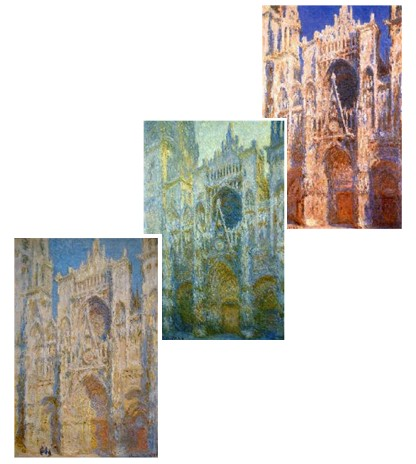
\includegraphics[width=12cm]{123BookCoverScreenshot_2022-01-23_141507.jpg}\\

%
\includegraphics[width=6cm]{赛希咨询.jpg}

\begin{titlepage}\thispagestyle{empty} \vspace*{3em}{\centering\Huge 软件开发过程改进(V01初稿) \par}\clearpage
\newpage \thispagestyle{empty} \mbox{} \cleardoublepage
\thispagestyle{empty} \vspace*{7em}{\centering\Huge 软件开发过程改进\par}{\centering-- 从个人到团队到公司from individual to team to organization \par}\cleardoublepage

%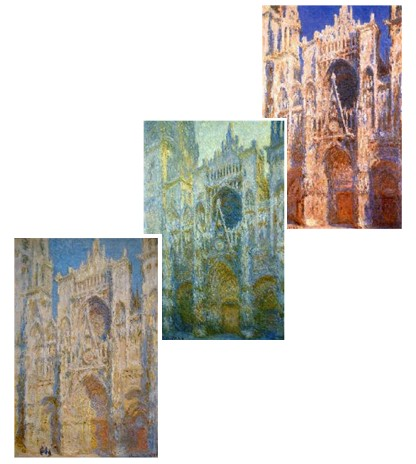
\includegraphics[width=12cm]{123BookCoverScreenshot_2022-01-23_141507.jpg}\\

%
\includegraphics[width=6cm]{赛希咨询.jpg}

\thispagestyle{empty} \vspace*{\fill} \parbox{.8\textwidth}{\raggedright \scriptsize
\textit{impossible} publisher 2022

printed blindfolded

design: \LaTeX
}
\end{titlepage}
\clearpage \thispagestyle{empty}\cleardoublepage
\newpage % Make sure the following content is on a new page

%----------------------------------------------------------------------------------------
%	TABLE OF CONTENTS
%----------------------------------------------------------------------------------------

\tableofcontents % Prints the table of contents

%----------------------------------------------------------------------------------------
%	INTRODUCTION SECTION
%----------------------------------------------------------------------------------------

\chapter*{前言 Prologue} % Introduction chapter suppressed from the table of contents

\begin{quote}
We are uncovering better ways of developing software by doing it and helping others do it.\\
--Agile Software Development Manifesto
\end{quote}

当今IT时代,软件开发越来越重要。但如何让软件开发也可以像其他工程领域,可以利用数字化来不断提升呢?\\
不少开发团队已经开始利用敏捷开发,两到四周迭代去对应客户需求不断变化。团队基于每迭代回顾、复盘其实可以利用数据,帮助进一步提升团队的质量与生产率。

本书主要是针对这点,借用一些实际的方法,场景,案例,让理解如何通过演化的过程,使个人到团队不断改善,包括:\\
1.制定方式/步骤/模型\\
2.针对问题的根因做试验\\
3.评判下一轮迭代的效果\\
4.利用数据,团队得到反馈,持续完善过程

这持续完善的过程,以前在工业生产年代已经被证明有效,Deming, Juran, Shewart等质量大师已经验证了这种改进方式,配合数据统计分析,可以提升生产线的质量与生产率。\\
如何利用这方式把作坊式的软件开发逐步变成有序的软件工程?

与工业生产不同,软件开发很多时候都无法像工厂收集到各种数据,但软件工程师仍然可以利用数据反馈做改进。很多软件工程师虽然开发能力很强,但未养成个人收集数据的能力和习惯,也不清楚如何用数据,持续改善。本书针对这些需求,以如何改善软件质量为目标,建议一些具体的做法、工具,帮助个人和团队可以立马尝试走出量化敏捷开发的第一步。

本书主要内容包括:

\begin{itemize}
\tightlist
\item
  从个人如何提升开始
\item
  如何基于个人的提升,演化成团队的提升
\item
  探索背后的一些管理思路,包括:

  \begin{itemize}
  \tightlist
  \item
    德鲁克
  \item
    敏捷开发 与 X-Y理论
  \end{itemize}
\item
  针对敏捷开发,如何利用度量与分析,不断提升质量\\
\end{itemize}


%----------------------------------------------------------------------------------------
%	BOOK PART
%----------------------------------------------------------------------------------------
\part{个人经验分享}我深信要提升必须源自个人,如果团队成员本身没有动力,团队无法提升。我虽然差不多天天都与软件开发团队打交道,但自己编码的时间很少,下面是相关的经验分享。\\


\chapter{个人学习Python编码} % Introduction chapter suppressed from the table of contents

第四天早上10:00我终于把所有功能写完并通过自动单元测试!\\
(老师说学编码必须动手,但我平时忙于工作,这次趁十一长假做编码练习题。上次做题已经是春节后,在集中隔离期间做过两题。这次的练习题只有十个功能,本来预计可两天完成。)

\framebox{%
\begin{minipage}[t]{0.97\columnwidth}\raggedright
练习题 (Problem
Set)------分析美国过去温度变化,提供了美国超过20个城市的每天平均温度。(从1961年到2015年)

\begin{itemize}
\tightlist
\item
  先写基本功能:

  \begin{itemize}
  \tightlist
  \item
    画散点图,回归分析,计算标准差与决定系数 (R\textsuperscript{2} Coef.
    of determination)
  \end{itemize}
\end{itemize}

\begin{itemize}
\tightlist
\item
  分析过去的五六十年数据,来判断美国或全球是否在暖化
\end{itemize}

给学生的文件包:

\begin{enumerate}
\tightlist
\item
  ProblemSet5.pdf : 分成 A、 B 、C、 D、
  E部分,详细说明每部分要开发的功能
\item
  PS5.py 程序模板,学员填入代码
\item
  PS5\_test.py 自动单元测试模块,自动测写好的PS5.py
\end{enumerate}\strut
\end{minipage}}


回顾一下,像我这种Python新手,因为不熟悉Python语言的属性与特性,必须按部就班,一步一步来写,欲速则不达。

更重要是体会到个人如何记录数据并分析:

\framebox{%
\begin{minipage}[t]{0.97\columnwidth}\raggedright
\hypertarget{ux8bb0ux5f55ux65f6ux95f4}{%
\subsubsection{记录时间}\label{ux8bb0ux5f55ux65f6ux95f4}}

十多年前我在美国考CMMI培训师,被观察时,
观察老师会在培训后告诉我,每一个模块用了多少时间,与计划对比。
从此以后每次培训我都会习惯记录每个模块所花的时间。

\hypertarget{ux600eux6837ux505a}{%
\subsubsection{怎样做}\label{ux600eux6837ux505a}}

培训时,我都会在桌上放一数字电子钟,记录每一个模块的开始时间与结束时间。上完一天课,晚上在电子表单计划时间旁边写上每个模块的实际时间。
这三天半,我也是用这种方式记录每个模块的时间。

\hypertarget{ux8bb0ux5f55ux7f3aux9677}{%
\subsubsection{记录缺陷}\label{ux8bb0ux5f55ux7f3aux9677}}

因为每个功能都很小,不到20行, 所以没有正式把缺陷与返工工作量记下来。
尤其是一些小的语法错误问题立马就改正了。
但影响较大的重大缺陷,我会记在模块旁边,算是这个模块花的时间。

个人记录实际时间没有想象中这么困难,
只要每天晚上简单按当天本子的数据更新电子表单,避免遗忘。
%will remove after jpg inserted
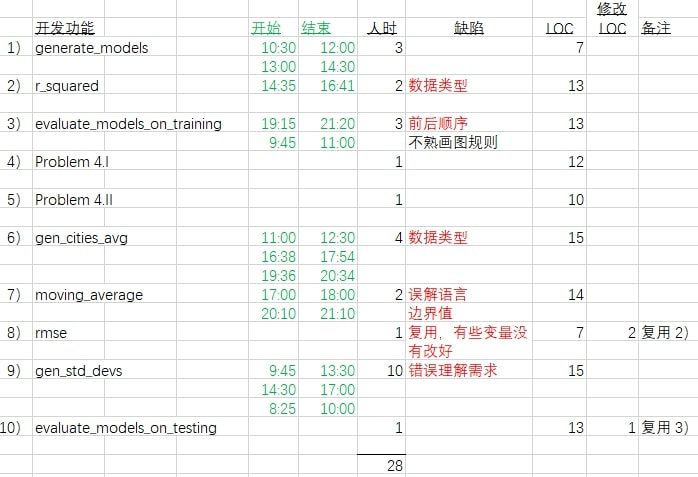
\includegraphics[width=12cm]{PspLogScreenshot_2021-10-06_174917.jpg}
\strut
\end{minipage}}



\framebox{%
\begin{minipage}[t]{0.97\columnwidth}\raggedright
\hypertarget{ux56deux987eux5206ux6790}{%
\subsubsection{回顾分析}\label{ux56deux987eux5206ux6790}}

整个编程结束后,写上每一个模块的实际代码行数。注意:如果模块是复用其他模块代码,便需要注明改动的代码行数。例如:evaluate\_models\_on\_testing13行只修改了1行。

分析:除了标准差模块(gen\_std\_devs)以外,其他功能都能在1-3个小时之内完成。

计算标准差的功能花了 10
小时,问题出在我编码时没有详细看需求。开始以为是求每个城市的温度标准差。
然后再求标准差的平均数。\\
测试不通过后,
也没有再看需求便假定求当年几个城市所有当年每天温度的标准差,还是不对。
到了第四天早上再看看 ProblemSet5.pdf
需求描述才知道我一直误解了这功能需求。

\texttt{gen\_std\_devs~~对应每一输入年份,返回一个数值,依据以下计算:}~\\
\texttt{~1)按输入的所有城市,计算当年每一天的平均温度(所有城市的平均)}~\\
\texttt{~2)计算当年每一天平均温度的标准差}~\\

所以如按我本来的算法,算一个城市是正确,但两个或者多个城市的时候,答案就比正确答案大。

针对这个计算标准差问题,一直以为是语法问题公式计算错误问题。
但我用一些简单的数据检验去,未能发现任何不正常。
来来去去都没有实际的进展,差点想放弃。

\hypertarget{ux7ecfux9a8cux6559ux8bad}{%
\subsubsection{经验教训}\label{ux7ecfux9a8cux6559ux8bad}}

我常常跟客户说,要做好需求评审,才能降低返工工作量。 这次编码实验的经验告诉我,如果前期过程有缺陷遗漏, 后面确实要付出很大的代价。(10小时返工工作量是评审平均2小时(1 - 3小时)的5倍,这案例还只是15行代码的小功能。在实际软件开发项目中,经验丰富的编码员应不像我这么笨,但估计因前面过程遗漏缺陷在系统集成后,测试才发现的返工量应也不止5倍!)

有了数据记录,这类宝贵个人经验便可以转化为改进(不仅仅是一个印象)。例如,可以把这些变成个人风险清单的检查项 
-\/-避免同类问题再发生。

\hypertarget{ux7ed3ux8bba}{%
\subsubsection{结论}\label{ux7ed3ux8bba}}

统计工作量与缺陷数据要从个人开始,并在回顾分析各种缺陷类型的返工量,找根因,制定对应措施,下次可以避免同类缺陷,我们才有动力继续收集数据。\strut
\end{minipage}}


\hypertarget{ux5176ux4ed6ux7f16ux7801ux7ecfux9a8cux6559ux8bad}{%
\subsection{其他编码经验教训}\label{ux5176ux4ed6ux7f16ux7801ux7ecfux9a8cux6559ux8bad}}

\begin{itemize}
\tightlist
\item
  最佳实践: 尽量用最小的行数完成功能

  \begin{itemize}
  \tightlist
  \item
    像Python这类成熟的语言,绝大部分的功能都已经具备
  \item
    尽量避免基础方法编写一个已有的功能(reinvent the
    wheel),除了耗费时间外,还会写多错多
  \end{itemize}
\end{itemize}

\begin{itemize}
\tightlist
\item
  写任何程序前必须先有自动化测试用例

  \begin{itemize}
  \tightlist
  \item
    虽然自己可以先想一些数据自己简单测一下
  \item
    但替代不了另外一个人写的测试用例。跑通才有信心程序正确
    (所以自动单元测试是使用最多的程序)
  \end{itemize}
\end{itemize}

\begin{itemize}
\tightlist
\item
  架构与设计很重要

  \begin{itemize}
  \tightlist
  \item
    校方除了提供测试脚本外,还提供了写程序的模板 (PS5.py)
  \item
    每个功能都明确,输入是什么,什么数据类型,输出是什么
  \item
    学员自己只需要填写实现的代码部分
  \end{itemize}
\end{itemize}

\begin{itemize}
\tightlist
\item
  先把握好新功能的用法与结果

  \begin{itemize}
  \tightlist
  \item
    前面发现不少缺陷,是因为不清楚某功能的用法
  \item
    在写代码之前,自己应开个沙盘,用小程序先试验一下这计算功能有什么参数,会出什么结果
  \end{itemize}
\end{itemize}

\begin{itemize}
\tightlist
\item
  先评审后测试

  \begin{itemize}
  \tightlist
  \item
    在跑程序之前,屏幕展示或打印出刚写好的代码,用铅笔在白纸上按程序的逻辑,从头思考一下每个数据的种类和中间的变化
  \item
    盲目地去跑程序或测试,最终只得出测试失败,但还不清楚错在哪里,如何修改。所以不如在跑程序或测试前,自己先动脑筋模拟一次,仔细想通每个数据的变化
  \end{itemize}
\end{itemize}



\chapter[克服拖延症]{锻炼高效: 克服拖延症}  % Introduction chapter suppressed from the table of contents

有位北京的技术总监问:现在我遇到最大的难题就是如何提升下面技术人员的能力,如果他们全都是高手,我就很轻松了,但实际上最多只有三分之一,其他都是中低水平。您接触过这么多软件开发团队,有什么好方案?\\
我说:我没有解决提升技术人员能力的银弹,但你可以听听我最近这故事:\\
:: = = = = = = = = = = = = = = = = = = = = =


\includegraphics[width=8cm]{小李图.jpg}

小李:你能够在一周内写完程序通过测试,并把整件事汇总成分享文章初稿发布很厉害呀。\\
我:其实你也可以做到。在《个人写程序并记录统计的一些经验分享》里,我只是写了与软件工程相关的重点,
但个人有没有高效率的习惯其实更重要。

我在五年前教授项目管理时参考过一本效率小册 {[}详见 Reference1{]},
这本小册罗列了99个小技巧,每个技巧都不超过一页纸,我自己也一直用这小手册提醒自己。

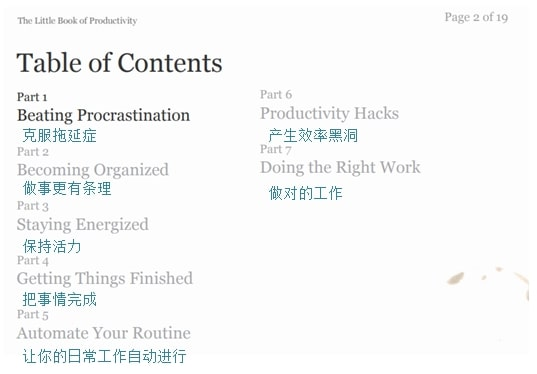
\includegraphics[width=10cm]{超效率目录.jpg}

例如,第一章``克服拖延症'',这里的几乎全部技巧有帮助:\\

\begin{itemize}
\tightlist
\item
  周 / 日目标 (1 Weekly / daily Goals)
\end{itemize}

\framebox{%
\begin{minipage}[t]{0.97\columnwidth}\raggedright
我每天都会定计划,早上希望完成哪些功能,下午完成哪些。当然这个计划也会按实际的进展调整。

周 /
日目标是个人时间管理的基本功。每一天第一件事不是回邮件,而是仔细想想今天要完成什么任务,每一周的开始,也应该想我本周希望完成什么任务。不然的话,每天的时间就很容易被琐碎的小事吃掉,一事无成。\\
\strut
\end{minipage}}

\framebox{%
\begin{minipage}[t]{0.97\columnwidth}\raggedright
背后的道理很简单, 要把时间花在重要、但非紧急的活动(下图右上角
)上,效率才会出来。

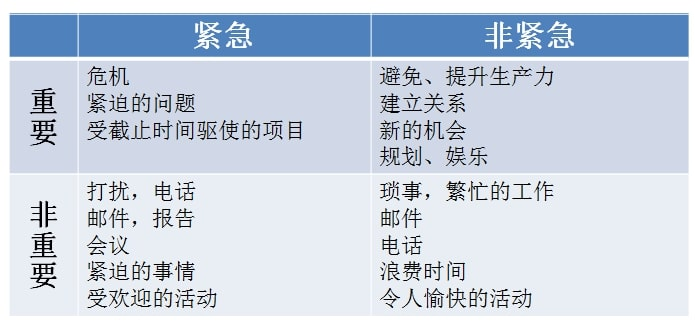
\includegraphics[width=10cm]{pfjp30.jpg}

\hypertarget{ux9650ux5b9aux65f6ux95f4-2-timeboxing}{%
\subsubsection{限定时间 (2
Timeboxing)}\label{ux9650ux5b9aux65f6ux95f4-2-timeboxing}}

把每天的任务安排成时间段,每一段不应超过1.5 小时。\\
一般人可以专心集中的时间段都不会超过60分钟,小孩可能就更短。如果老师叫你星期五5点钟交卷,你不会3、4点就交,都会等到最后十分钟,甚至五分钟。所以如果我们把一天的时间切开成
1 ~ 1.5 小时时间段,自然有动力, 希望在时间之内完成任务。\\
我们写代码的时候应该也是用同样的原理。例如。前面那个总共花了10个小时的功能,也是本身尝试了很多次。每次当我发现超过了1小时或者1.5
小时,我就会把它放下来,先做其他事。

\hypertarget{ux5206ux89e3ux4efbux52a1-3-dissolving-tasks}{%
\subsubsection{分解任务 (3 Dissolving
tasks)}\label{ux5206ux89e3ux4efbux52a1-3-dissolving-tasks}}

因为都是练习题,所以每一个功能都比较细,不会超过二十行。如果我们平常做开发时,也必须要把一些大、复杂的功能预先拆分成小的功能才有效率。\strut
\end{minipage}}

\hypertarget{ux52a0ux5f3aux81eaux5f8b-6-building-self-discipline-muscles-ux6668ux793c30-morning-rituals-ux65e5ux5e38ux8fd0ux52a8-32-make-an-exercise-routine}{%
\subsubsection{加强自律 (6 Building Self-Discipline Muscles), 晨礼(30
Morning Rituals) 日常运动 (32 Make an Exercise
Routine)}\label{ux52a0ux5f3aux81eaux5f8b-6-building-self-discipline-muscles-ux6668ux793c30-morning-rituals-ux65e5ux5e38ux8fd0ux52a8-32-make-an-exercise-routine}}

不要以为编码是一个单纯的脑力活。整天坐在电脑前面敲代码就可以,如果人的体力、精力没有配合上也会出问题,好在我每天早上一直坚持三十到四十分钟的轻量运动,然后晚饭前半个小时到一个小时的骑单车或者慢跑的习惯。中间也是不是整天坐着,一段时间会走一走,喝橙汁等,确保身体不断在动,才不会困,保持动力。

贝多芬每天都会去外面散步,来启发一些创作的灵感,然后他会立马把这些写在本子上,用于后面的音乐创作。早上的跑步也可以让我有多些创作灵感。

\hypertarget{ux4e0dux4f1aux5206ux5fc3ux7684ux5de5ux4f5cux573aux6240-11-create-a-distraction-free-workplace}{%
\subsubsection{不会分心的工作场所 (11 Create a Distraction-Free
workplace)}\label{ux4e0dux4f1aux5206ux5fc3ux7684ux5de5ux4f5cux573aux6240-11-create-a-distraction-free-workplace}}

\hypertarget{ux8f7bux7b56ux5212ux8fedux4ee3ux518dux7b56ux5212-13-ready-fire-aim}{%
\subsubsection{轻策划,迭代,再策划 (13 Ready , Fire,
Aim!)}\label{ux8f7bux7b56ux5212ux8fedux4ee3ux518dux7b56ux5212-13-ready-fire-aim}}

三十年前,软件开发都是很大型的一些项目,整个架构要设计好才动手去写代码。现在反过来,需求变化极大,开发都需要敏捷,轻文档轻计划。尽快写好代码,做一些功能给客户,从反馈优化下一轮。我这次的几天开发也是用同样原则,没有花时间在一些设计或者文档。想直接把那个代码写出来,并通过单元测试,就节省很多耗时间的工作。把有限的时间都放在写好代码上。

\hypertarget{ux4e0dux65adux6e05ux6d17-10-churning}{%
\subsubsection{不断清洗 (10
Churning)}\label{ux4e0dux65adux6e05ux6d17-10-churning}}

万事开头难。我在开始的半天也是遇到同样问题,不知如何入手,太久没看写代码的书了,很多基本的都不知如何入手。所以我开始的时候不会直接尝试写题目里面的功能,而是重写一些书本的代码,看看跑出来怎么样,然后逐步提升。写一些基本功能,慢慢有了习惯,调整过来了,后面就越来越顺。好比一台旧的水泵,刚开始抽上来的水总是有难喝的铁锈,只要不停止抽水,当污水最终都从系统中抽出后,就能发现底下的净水。

\hypertarget{ux8981ux6709ux597dux7684ux571fux58e4-8-remove-your-hidden-roadblocks}{%
\subsubsection{要有好的土壤 (8 Remove your Hidden
Roadblocks)}\label{ux8981ux6709ux597dux7684ux571fux58e4-8-remove-your-hidden-roadblocks}}

在含盐量高的土壤里种植物,是结不出果实的。浇水、平衡在阴凉处和阳光下的时间都抵不过根部吸入的毒素。如果我们没有积极性,就可能是土壤的问题。如果没有足够的积极动力,就不会在长假专注写程序,也不会定期要求自己写分享文章。所以要有明确/很想达到的目标驱动。
像一个作曲家,他希望写出很多经典的优秀作品,不满足于现在的状态。觉得自己的灵感或者创造力没有发挥出来,成为可以保留下来的东西。也是这种驱动力让我可以一直努力做这件事。\\

\hypertarget{ux6452ux5f03ux62d6ux5ef6ux6076ux4e60-14-quit-your-procrastination-vices}{%
\subsubsection{摒弃拖延恶习 (14 Quit your Procrastination
Vices)}\label{ux6452ux5f03ux62d6ux5ef6ux6076ux4e60-14-quit-your-procrastination-vices}}

长假里,大部分人都会把时间用于看视频或电视剧,而我正好没有这个习惯,也一直没有玩网络游戏的习惯,否则肯定完成不了。

最终我用日程记录(91
Timelogging),把整件事和什么活动、时间花在什么地方都记录下来了。

小李:我看你上面列出的技巧,我大部分都还没做到。

我:不要紧,我六年前刚开始定期写文章时情况跟你类似,但只要不放弃,一直往既定目标努力,不良习惯都改正过来了。

我常常说人的潜力是极大的。 舒伯特你听过吗?\\
小李:好像是一个很有名的作曲家。\\
我:是的,但他很年轻31岁(1828)
就去世了,你猜他一生一共写了多少首歌和音乐作品。\\
小李:我记得中学时,老师介绍过他的艺术歌曲,如``鳟鱼 The
Trout'',但他31岁就死了,我猜100 - 200 首歌?\\
我:他一生写了超过460首歌曲(时长\textgreater{}24小时)。除了歌曲,他还写了其他作品,如9首交响曲,20
室内乐,120 钢琴曲等等,每一类都包括大量经典作品,对后世影响深远。\\
小李:如果粗算他一生600作品,算他有16年时间作曲,平均每月要完成3个作品,真是不得了。\\
我:虽然他的作品有大有小(从一首歌,到45分钟的交响曲),他确实生产率极高,而且他最后的7年一直身体都不好,所以他那个时候肯定不会像我们现代996方式工作。
他每天主要是早上用来写作,傍晚便去休息散步。但他会同时做多个创作项目 -
那些项目没有灵感,就暂时放下来,创作其他作品。
他著名的未完成交响曲就是个好例子,只有两个乐章(一般交响曲都是四个乐章)
所以他是使用高效技巧的一个成功例子。

每个人都有自己的理想,但如果没有高效率来执行,理想只是天马行空,天方夜谭,不会有任何成就。有没有疑问?

小李:没有,挺好的,我后面立马就开始。\\

总监说:我大概懂你的意思了,要提升技术人员的能力先要改变他们的习惯,有良好的习惯(如时间管理),才有机会提升。\\
我:是的。\\
总监问:从管理者的角度,我们有什么可以做的?\\

\hypertarget{ux5373ux65f6ux7b14ux8bb0-17-the-capture-device}{%
\subsubsection{即时笔记 (17 The Capture
Device)}\label{ux5373ux65f6ux7b14ux8bb0-17-the-capture-device}}

总监边听边在本子上记下那些重点。高效的人都会有工具帮他记录想到灵感、想法、项目、待做事项等等,不会仅仅靠大脑记忆。你提出一个要求,他会立马写在小本子上,你会觉得他应该会按你要求去处理,但反过来他只是口头说会处理,你会担心很可能没有下文。但我看有些领导,身边只拿个手机,除非他们的记忆力超人,不然话我估计他每天都会忘记不少重要事项。

下一篇,我们将讨论如何从个人上升到团队的提升。\\

\hypertarget{ux676dux5ddeux9ad8ux7ea7ux7ecfux7406ux53cdux9988}{%
\section{杭州高级经理反馈}\label{ux676dux5ddeux9ad8ux7ea7ux7ecfux7406ux53cdux9988}}

人一定要自律!您说的小技巧确实能起到很大帮助,而且我基本都会使用,但如果不养成习惯,想起来使用下,最终还是改不了拖延症,所以要解决拖延症,一定从根源做起,还是得靠自己,需要培养自己意志力、专注力,坚持好习惯,改掉坏毛病。\\

\cite{prod1References1}
 %from individual to team
\chapter[从个人到团队]{锻炼高效: 从个人到团队} 

个人精力有限,必须借用团队才能成倍提高生产率。但不能仅靠组长个人的努力:例如有些开发技术出身的组长,自我时间控制很好,技术也不错,但不懂如何有效下放工作,协助团队成员,导致团队不懂,做不出来,最后组长就自己动手搞定,恶性循环。
所以团队要有效率,除了依赖个人能力外,还需要了解高效团队的挑战。

\framebox{%
\begin{minipage}[t]{0.97\columnwidth}\raggedright
知识工厂 (Knowledge Factory)

一位老同学在东莞有一个"知识工厂",主要是为美国客户服务,输入扫描件,输出修正好的、正确的英文文件。\\
因为美国的人工费用很高,所以客户愿意把一些耗费人力的手工工作外包。\\
虽然公司可以利用识别英文字的软件把扫描件转化成电子版,但只能做到大部分,还是有很多地方需要看原文,手工输入、修正。这个知识工厂就是找一些初中学历的人,经过简单培训后上岗,把编辑好的文档发回给美国客户。一般是按字数收钱,因为是外包业务,利润非常低,所以必须要控制生产效率------如果效率低工厂就不赚钱了。但效率不仅仅是速度,如果有太多错误,客户便不满意,所以也要控制质量。\\
\textbf{典型客户}:\\
*某网站服务,收集了大量老资料,专门帮助美国人寻根。

\begin{itemize}
\tightlist
\item
  例如某美国人可能前几代是从爱尔兰过来,但只知道是哪年哪月,他可以从这网站搜索某时间段轮船的客户名单,所以这公司便需要把大量老轮船客户名单,转换成电子文件,其中也会遇到很多古老的字,扫描软件难以识别。
\end{itemize}

有一天他邀请我去参观东莞分厂,办公大厅里有很多人,大家头戴耳机在屏幕前敲打键盘。\\
员工每 7 - 10
人分成一个小组,每组一个组长,每组头上有个大屏幕,显示着数字。\\
我就问同学这是干什么的,他说这些就是反应每个小组当前的速度,每个组员都可以看到,效果就是让成员们能直观看到工作的反馈:现在整个组的速度、质量如何,都可以从那些数字简单地反映出来。\\
我老同学说:\\
``每个员工和团队都很清楚当前的效率和质量。
从这么多年数据显示,一般新员工经过培训后开始 1 分钟是 55- 85 WPM(Word
per Minute )。
但因为经验少,所以一般错误率比较高。经过几个月的实际工作,速度和准确率都会有提升。我们提拔组长也主要是看他过去的指标是否领先。\\
除了监控,我们也会完善一下新的系统来帮助团队,例如,系统会同步给他们一些提示,也会用语英语读出来,帮助他们更好完成任务。``\\
\strut
\end{minipage}}

以上是团队如何利用系统,提高生产率和质量,让公司盈利生存的例子。
我立马想到,如果没有及时的数字反馈,很难让团队知道自己现在的状态。这跟我每天早上跑步一样,如果没有计时,就没有动力保持或超越以前的速度。\\
克服拖延症里面提过的效率小手册第二章里的“做事要有条理” (Becoming Organized)
如果个人无法把所有所做的事情清晰地分解,就很难有效率。比如,小手册提了几点简单的组织系统帮我们:

\begin{enumerate}
\tightlist
\item
  分成项目 (20 Projects)
\item
  项目由任务组成 (21 Tasks)
\item
  任务或活动,要有开始日期,结束日期 (22 Events)
\item
  分支法 (24 Branch)
\end{enumerate}

一个人要管理一个团队,当那些任务不是仅仅是自己看和做,而是要分摊到团队其他人去完成的时候,就更需要有个系统,让大家看到计划与实际。在项目管理来讲,这个叫工作任务分解
(Work Breakdown Structure WBS)。

我在北京给一家公司做评审时,问他怎么管理项目,他很自信的说跟你上次见不一样了,我们现在有项目管理系统。

其实他说的管理系统只是一个任务管理系统(类似缺陷管理,每一个缺陷或任务独立,然后就让成员填写任务的完成情况)。因为系统只能跟踪任务的实际完成情况,没有WBS分解能力,难以管理整个项目。可以想象,如果项目有一百多个任务,经理怎么知道任务的进展情况呢?只能看到每个任务状态。但是如果能把任务按过程(如测试,编码),模块(如
A模块、B模块等)或迭代分组,我就可以把那100多个任务汇总成5、6个组,经理或团员就可以从系统中得知项目的情况。

:= = = = =\\

某家做保险系统的国际公司,因为要控制人手,所以采用了外包模式,让顾问公司提供人员来现场做开发,公司内的项目经理手下可能有五、六十人在工作。
以前,他要监控这些开发活动时,需要去检查每个人的情况,忙不过来。
这就可以用一个 WBS 管理的系统,来全局监控开发的情况。
WBS项目管理系统如何帮到这个项目经理呢?
项目管理系统要求每个任务(或工作包)都需要有产出物,而且产出物必须通过评审才算百分之百完成。这样的话项目经理就不需要逐个产出物自己查看了,他可以安排团队自己相互评审产出物,项目经理就可以总体监控项目进展,提高团队效率。\\

:= = = = = =

有些高层也了解项目管理有不足,但觉得是流程的问题,要求先把流程建好,才上自动化系统。这种思路听起来很有道理,但实际上行不通。

原因是过程跟系统是息息相关的,如果没有系统,你的过程只是基于一堆手工模板,无法操作,就好比你可以用excel表希望做项目管理系统一样。原因是那些excel表它不是一个系统,最大的问题是它可以随时更改结果,所以这种系统出来的报告,都是说没有偏差。对监控项目没有作用。
我们后面就用一个实例看看怎么在开始的时候可以尽快尝试一下怎么用一些系统来帮我们管理个人的小项目,因为我们说所有过程改进都应该先从小的试点开始。

现在我们都流行用SaaS系统(Software as a
Service),所以很多服务都可以在线上直接使用,不需要预先安装服务器,数据库,应用软件,配置等等。比如我随便进一个这类的WBS项目管理系统,我输入这两周主要的一些主要活动,如:

\begin{itemize}
\tightlist
\item
  用水晶球完善预测模型
\item
  完善国际功能点教材与资料
\item
  为简化功能点准备一套资料,让公司可以开始使用
\end{itemize}


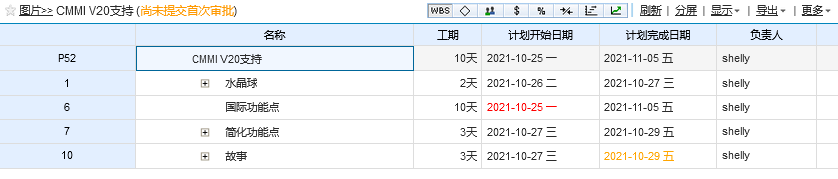
\includegraphics[width=10cm]{微信截图_20211029132308.jpg}

因为我都在外面忙,我只是可以把这些重点设出来。然后每天会议要求做的人在里面添加活动:

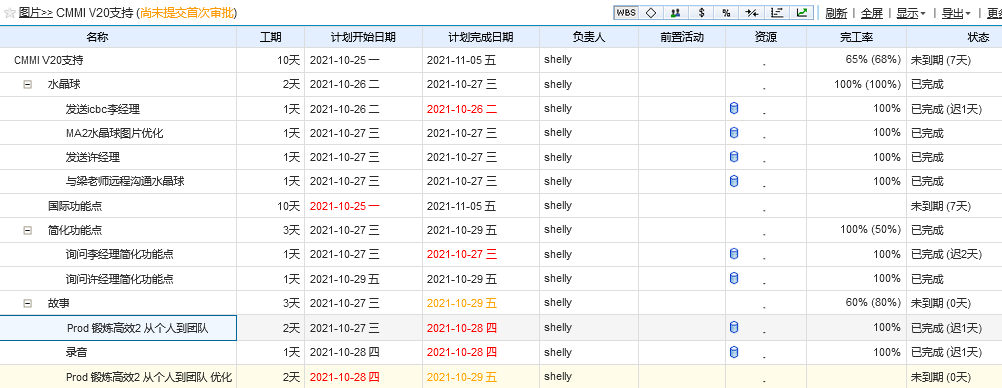
\includegraphics[width=10cm]{微信截图_20211029090316.jpg}

因为它是一个SaaS系统,所有团队的成员不一定是在同一个办公地点,都可以看到,还可以上传任务的产出物,并看到任务的完成百分比。

每周五,各人在系统填写实际工时(注意:在她填写实际工时的时候,能看到每活动的计划工时):


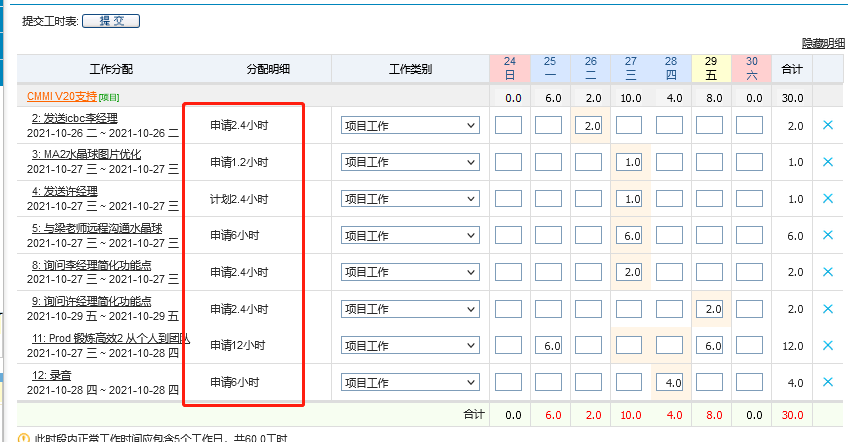
\includegraphics[width=10cm]{微信截图_20211029090520.jpg}

在没有做这个之前,我也尝试过在大白纸上面每人写上当天和每周的活动,要团队每天下班拍照发我,但发现一点用都没有:

\begin{enumerate}
\tightlist
\item
  我没时间去看里面有没有具体的时间、工作量
\item
  缺乏数字性记录
\end{enumerate}

我开始用这个系统后,两个月过去,就可以有一些统计数据,从系统里面可以抓出来团队或者个人在过去这个时间完成了什么任务,因为都在系统有记录,也因为有产出物,我用Wiki
跟踪这些产出物的话,我就可以在 Wiki
里面记录每一个产出物的缺陷,所以也可以得到每个人或者团队的质量。把本来只是我个人的管理,扩大到团队管理。


 %
\part{再读德鲁克与 X-Y 理论}要提升软件开发质量与生产率,敏捷开发不是必赢的灵丹妙药,有人说敏捷就是精益(LEAN),虽然LEAN是敏捷的重要部分,但不是全部。想要合适地使用敏捷帮助团队提升,便要先了解敏捷开发背后的管理思路。\\

从50年代起,管理学开始探索如何能提高员工的生产率和质量, 发现传统的军队式管理,和工厂式生产线模式不再合适, 提出要让团队自主,管理者要抛开家长式管理的思维,提出X-Y理论。\\

从60年代到90年代,各行各业不少公司,如服务页(酒店),生产等,采用这新思维,取得显著效果。 2000年,17敏捷领结大师,觉得当时美国软件开发有很多严重问题,提出敏捷宣言, 其实背后的管理思路已经有五六十年历史, 下面我们先从现代管理学大师德鲁克先生的一些文章开始, 然后借用我一些教敏捷ACP 用的故事,介绍X-Y理论与敏捷开发的思路。\\

如果读者想多了解敏捷开发,可参考附件 ‘Agile Primer’。 \\
\chapter[如何提升生产率]{再读德鲁克: 如何提升生产率} % Introduction chapter suppressed from the table of contents

\framebox{%
\begin{minipage}[t]{0.97\columnwidth}\raggedright
一家500人的北京IT公司,专门做企业大数据服务。为了加强管理,他们利用项目管理系统做项目挣值分析(Earned
Value),要求团队先做预算,然后按项目任务完成情况报工,监控实际与计划对比。这就是典型传统会计成本监控。监控已发生的任务,但无法帮我们避免一些可能发生的风险。\\
我问技术总监:``你们公司的核心竞争力是什么?''\\
答:``我们的开发团队都很有经验,开发质量也满足客户要求。''\\
问:``你们如何衡量开发团队的质量和生产率?''\\
答:``我们半年前开始利用项目管理系统,每个月按照项目是否有超时或超出预算。''\\
问:``生产率不等同于项目是否延期,其实与同行相比,你们已经算不错,很多其他企业连这些项目基本监控都缺乏,但如果你们也衡量软件开发团队的生产率和质量,你们会更清楚自己是在什么水平?是否在进步?如果你们有团队的生产率和质量数据,你便更好监控项目,可以从团队的生产率和质量数据预测项目可否按期完成。''\strut
\end{minipage}}

如果我们想知道有什么好方式帮助软件开发团队提升生产率,可先回看上世纪人们如何提升工业生产率。

在20世纪初,科学管理的先行者泰勒(Frederic TAYLOR)
先生开始对劳动者做任务分析和管理,研究各个制造业工人的工作,记录劳动者每个动作,和完成动作的体力和时间,研究如何去除多余的动作。

他的结论是:无论什么工作,都是重复性,如果把那些步骤写下来,任何人不需要什么特别训练,熟练后都可以成为一流大师。\\
当时他的理论被不少美国工会强烈攻击,很简单,当时很多兵工厂都有工会,学徒制,要入行必须当多少年学徒,还也要有熟人推荐才进得来。为什么这么刁难,原因很简单,如果你可以最后当成那些兵工厂的领班或工人,你的薪水可能比医生还高。\\
可能是这个原因,二战时,希特勒在日本偷袭珍珠港以后,错误地认为美国不能在短间可以追得上德国的工业化程度,他就决定跟美国宣战,(宣战前美国,因有内战痛苦经历,国内反战声音巨大,导致在一战时几乎都没有参战,不重视发展军工,缺乏军工方面的人才,比如缺乏军用设备(如光学、镜片)的专业技工)。但事与愿违,美国借用了泰勒先生那一套方式,快速建立兵工厂,大量生产飞机、坦克等等设备,生产力后来居上,超越了德国、日本,最终获得二战胜利。\\
20世纪,制造业的体力劳动者生产率增长了50倍{[}2{]},但现在大部分已发展国家,传统的工业生产只占总生产的小部分,大部分是服务业或知识工作。

所以在21世纪,我们的新挑战是如何能同样提高知识工作者的生产率。

\hypertarget{ux4efbux52a1ux662fux4ec0ux4e48-define-the-task}{%
\subsection{任务是什么 (Define the
Task)}\label{ux4efbux52a1ux662fux4ec0ux4e48-define-the-task}}

知识工作与体力劳动不同,知识工作者的工作大都不是预先安排好。比如汽车生产线,工人只需要按照程序安装组件就可以,劳动者只问``怎样做才能做得最好?''。但知识工作中,知识工作者主要问``任务是什么?''。

\framebox{%
\begin{minipage}[t]{0.97\columnwidth}\raggedright
100多年前,20世纪初,当时没有互联网,没有电商。如果你不想亲自去百货公司买东西,你可以把钱寄到百货公司邮购,但这需要很多人手数寄来的现金。当时"SEARS"百货公司,
不采用传统的数钱方式,用磅来称寄来邮购信件有多重,从而判断里面有多少硬币,多少钱,连信封也不打开。这种方式就可以大大减少所需的人手,在短短两年间,把这一块服务的生产率提高十倍。\strut
\end{minipage}}

如果保险公司也问:``任务是什么?''
答案应是``对死亡申请赔偿要尽快,也最省钱。''

\framebox{%
\begin{minipage}[t]{0.97\columnwidth}\raggedright
保险公司本来每次有事发生,客户要补偿时,保险公司传统都要检查三十个以上不同条件。\\
为了增加生产率,保险公司决定只检查以下关键4项:\\
一、这个保险单是否还有效?\\
二、他申请的金额是否与合同匹配?\\
三、那个人名跟那个死亡证是否对应?\\
四、受保人是否对应?\\
最终把本来要平均十五分钟的事情减到三分钟。

现在很多保险公司只对百分之二的抽样做控制,i.e.只对五十分之一的索偿完整地检查所有项,其他都是按上面这种快速方式处理。\strut
\end{minipage}}

医院也可以利用问``我的任务是什么?''这个问题来提高服务的生产率。很多医院花很多时间要求本人填写的资料,进医院前。甚至有些病人,急诊的病人,因为他们可能已经不清醒,无法填写很详细的表格。如果我们用刚才那个问题,这答案是,入院的手续最重要的是希望识别病人的姓名、性别、年龄、地址和如何收费?就是在一个病人,他的门卡上面有的信息。用这个方式可以大大简化入院服务,生产率也自然提高。

所以在服务业我们要增加生产率,最重要不是像以前劳动工人那种看他每个步骤,更重要的是你要想你的任务是什么?\\

\hypertarget{ux4e13ux5fc3ux5de5ux4f5cconcentrate-on-the-task}{%
\subsection{专心工作(Concentrate on the
Task)}\label{ux4e13ux5fc3ux5de5ux4f5cconcentrate-on-the-task}}

另外一个常常影响服务生产率的问题是不能专心集中工作,例如很多医院都说缺护士,但其实每年都有不少的新毕业员工加入,病人也没有大量增加,为什么会人手不够呢?\\
其实很多浪费是由于护士不是做本职工作``护理病人`,而是花了大部分时间在填写报告,而非医护工作。\\

高校老师也一样,主要任务本应是教学生,但其实花了很多时间开会,例如一些委员会会议。\\
销售人员也一样,不是专注与客户沟通,而是花很多时间在无谓的内部会议,填写报告。很多销售员,平均每天起码花不低于三分之一的时间在这类客服工作,跟销售无关。\\
所以每个行业服务人员都应该问这个问题:``我们受聘主要是要干什么的?我们这个工作主要提供什么价值?''\\
比如某百货公司,员工的回应是``销售''。但其他百货公司,可能是"客服"。所以针对不同的目标,公司应该回顾整个团队是否花了很多时间做一些没有价值的工作。\\

\hypertarget{ux4e0dux80fdux5355ux770bux6570ux91cfux8d28ux91cfux540cux6837ux91cdux8981define-performance}{%
\subsection{不能单看数量,质量同样重要(Define
Performance)}\label{ux4e0dux80fdux5355ux770bux6570ux91cfux8d28ux91cfux540cux6837ux91cdux8981define-performance}}

除了问工作是什么以外,也要问怎么做才有效?

比如一个建筑绘图员,不仅仅衡量图的数量,也要取决于他绘图的质量。其他服务,无论是工程、银行、医院、报社也一样。

例如,药厂实验室科学家,质量最重要,数量其次:如果能研发一个一年销售50亿的``明星''药品,肯定比一年发明超过50个`一般'药品
(年销售2000\textasciitilde{}3000万)好。

\hypertarget{ux56e2ux961fux6709ux81eaux4e3bux6743ux81eaux6211ux7ba1ux7406partnership-with-the-people}{%
\subsection{团队有自主权,自我管理(Partnership with the
People)}\label{ux56e2ux961fux6709ux81eaux4e3bux6743ux81eaux6211ux7ba1ux7406partnership-with-the-people}}

1.定义任务\\
2.专注\\
3.定义性能质量\\
如果我们能一步步完善以上三点,就应该不难,与上一个世纪一样,大大提高服务的生产力。

以上3点能否有效,取决于管理者能否把知识工作者当成``资产'',而不是``成本''。

不能再像以前,把工人只是当作一双手,知识工作者要与前线人员团队合作,才有效。有不少公司,比如IBM一直都有已经采取这种方式多年。日本的工业也一样,本来企业家以为可以继续用二战前那种专制的管理方式,但引起很多罢工,后面也改了。在以前工业生产时代,管理者与前线团队互相合作,支持他们只是一种最佳实践,但现代,这是唯一的方式。

\hypertarget{ux5b66ux4e60ux73afux5883learning-environment}{%
\subsection{学习环境(Learning
Environment)}\label{ux5b66ux4e60ux73afux5883learning-environment}}

管理者要支撑支持前线人员组成自主团队。让他们不断改善服务,达到目标。现代,业务环境快速变化,服务人员也要终身学习才跟得上。培训只是开头,更重要的是他们如何把学到的用于工作中。如果每个人都当内部讲师,不仅仅其他员工受益,讲师本身也受益,进步。比如,找某明星销售人员,让他在全国的年会分享成功经验,教大家怎么做好市场工作,培训过程中,他自己也会思考那些是成功要素,更进步。

\hypertarget{ux5bf9ux8f6fux4ef6ux5f00ux53d1ux7684ux542fux53d1}{%
\subsection{对软件开发的启发}\label{ux5bf9ux8f6fux4ef6ux5f00ux53d1ux7684ux542fux53d1}}

你觉得以上德鲁克先生在1991年针对如何提升知识工作者生产率{[}1{]}的建议,适用于软件开发吗?
下面每一点看看:

\hypertarget{ux4efbux52a1ux662fux4ec0ux4e48}{%
\subsubsection{任务是什么}\label{ux4efbux52a1ux662fux4ec0ux4e48}}

上面的例子:处理保险申报、百货公司邮购等,都是精益(Lean)概念,把有限精力放在最有价值的东西,减少浪费。
2000年,17位软件开发大师针对软件开发问题,如项目延期、失败等问题,发表了敏捷宣言,包括:

\begin{itemize}
\tightlist
\item
  不浪费时间写一些对客户没价值的文档,专心写好代码。
\item
  不浪费时间做一个三个月的详细项目计划。而集中精力把后面两周可以做到什么详细计划好。
\item
  每一轮两周冲刺后,与客户沟通,得到反馈才知道哪些开发出来的是对客户有价值,哪些不是客户要到便立马停止。不像以前等到整个瀑布式开发,最终交付才知道。
\item
  极限编程(eXtreme
  Programming,敏捷的一种)提倡测试驱动开发TDD,道理也一样,如果你这个小程序模块,没测试好就集成到整个系统中,后面会产生很多无谓的返工,必须每个模块都先测试好。
\end{itemize}

这些背后都是精益,越来越多软件研发项目使用敏捷开发。\\

\hypertarget{ux4e13ux5fc3ux5de5ux4f5cux4e0dux5206ux5fc3}{%
\subsubsection{专心工作,不分心}\label{ux4e13ux5fc3ux5de5ux4f5cux4e0dux5206ux5fc3}}

最近周末抽空编写Python小程序。\\
但因很久没编码了,所以一天能完成的程序不多,几十行代码。但发现编写程序需要很高的专注力,原因很简单,写文章就算有错别字人家还可以看得懂,但写程序错了一个字就跑不通了。所以我每写一段代码都会依据TDD原则,写十来行就用一个小模块就去测试。这样才可按计划完成当天要完成的练习题。\\
所以不要分心这点在软件开发特别重要。\\
但很多开发人员都要同时兼顾4-5个项目,还要维护一些老项目的出厂后的缺陷,其中有些更要紧急处理。可想象这些开发人员如何能专心写好程序?但不专注便很容易引起后面返工。\\

\hypertarget{ux786eux4fddux8d28ux91cf}{%
\subsubsection{确保质量}\label{ux786eux4fddux8d28ux91cf}}

如何提升软件开发质量?最终还是取决于代码质量。如果代码本身写不好,测试多完美,质量不会好到哪里。需求没做好也是常常影响质量的问题,大量的变更也会影响代码质量。

不要以为把质量做好,会影响生产率。其实生产率不会下降,反而会提高。(
我们过去几年利用量化敏捷管理帮助一些敏捷团队,确实验证了我们帮助团队注意,提高代码质量,降低交付后的缺陷率,生产率没有下降,反而提升。)

所以管理者必须重视并关注软件开发质量。

\hypertarget{ux600eux6837ux8861ux91cf}{%
\subsubsection{怎样衡量}\label{ux600eux6837ux8861ux91cf}}

怎样衡量保险公司,百货公司,药厂等的生产率都很明确,
但如何衡量软件开发生产率一直有争议,大家只知道不应该数代码行数。\\
如果你请开发团队对一个新的开发项目做估算,他们听完需求后告诉你,估计需要三到四个人月。\\
但人月不是规模大小,它是工作量。 这表示估算时已经假定了团队的生产率。\\
也正因为没有衡量规模,导致软件开发团队没有提升生产率的动力,为什么?\\
道理很简单,如果同样开发一新软件,某团队创新新方法,可以把三个人月的工作减少到两个人月,但客户不会给你三个人月的钱,因为你只用了两个人月,只按两个人月付费。\\
没有度量就没有管理,所以必须要能衡量软件规模,才可以谈如何提升生产率。\\
前面提到敏捷能精益原理帮助软件开发提升,但如果你问敏捷开发团队过去几年生产率提升多少?我估计你得不到答案。原因是敏捷从2000年开始,都集中说编码开发的最佳实践,缺乏可比的规模单位。\\
很多敏捷团队使用故事点(Story
point),但一个公司的故事点跟另外一个公司的故事的无法比较,甚至一个公司里面团队A跟团队B之间的故事点也比不了。\\
但如果使用功能点估算规模,团队之间的生产率,缺陷率等便可比。\\
你可能问``功能点我们都听过,其实七十年代都已经出来了,但会如果你说的这么好,为什么这么多年都不能在软件行业普及?''\\
原因很简单,本来的传统功能点如 IFPUG 、
NESMA,主要用来结算,不是用来估算。结算就是当你已经完成产品开发,按每一个页面有多少输入输出,多复杂等等,计算算这个软件的规模大小。但实际上,在现在这个千变万化的年代,你有多少项目可以一开始就有明确需求?绝无仅有。大部分时候,客户也不一定完全了解他要什么,只可以说给你一个大致的概念,常需要用一两个月时间逐步的边开发边了解,逐渐明确。\\
所以团队很难使用传统功能点,来做规模估算;但近几年,使用功能点结算越来越及,很多政府已经规定使用功能点来客观衡量软件规模大小。\\
针对传统的功能点算法难以用于早期项目估算这困难,我们有一套量化敏捷开发方法(类似简化功能点),按照需求的``实体''数和``行为''数做规模估算,补充敏捷开发缺乏可比规模的不足。估出来功能点虽然与传统功能点数有偏差,但因敏捷每冲刺只是2-4周,精确度不需要像以前瀑布式开发那么准。\\
现在科技发达,越来越多工具可以帮我们在开发完以后,从实际的开发完的代码去反过来算这个项目的实际功能点数(算实体、行为有多少)。\\

\hypertarget{ux603bux7ed3}{%
\subsubsection{总结}\label{ux603bux7ed3}}

有些软件开发公司可能一直收集很多缺陷统计、工作量统计、进度统计等,但是如果缺乏规模,还是无法判断生产率和质量。所以这个是软件开发规模度量提升生产力的第一步。\\
有度量,便可以尝试创新和改善,例如自动化。\\
有些公司已经开始探讨用自动化测试去提升生产率。我们的经验是,不少公司还是半途而废,最后失败。

如果高层有很高要求,例如不能增加人手,生产率便必须提高,这种环境导致团队必须转成自动化,自动化测试便会成功,但反过来,测试说千万个理由,很难用自动化,测试人员继续增加,越来越多反对声音,长久还会回到手工测试,生产率难以提升。正如德鲁克先生所说,如要有提升,必须抛弃老的方式,终身学习,把自己的技术提升。更重要是管理层有很高的要求
和 坚持。

\cite{drucker2References1}
\cite{drucker2References2}



 %done
\chapter[再读德鲁克]{信息挑战}  % Introduction chapter suppressed from the table of contents

"这一两年,我们的VIP客户都已经数字化智能化管理了,我们公司管理是否也应朝这方向?''
一家二十年都一直专注通信行业的软件公司CEO问公司总监。

大数据分析已在各行业得以应用, 让企业可以数字化智能化管理, 提高竞争力。

数据在各行业越来越重要,
虽然不少软件公司已经摆脱了作坊式管理,正逐步改善规范,
但在数据的采集和使用方面还存在很多的问题,
不知道如何采集数据,以及如何分析采集到的数据。

别人的方法未必适合自己,那我们应从哪些方面来找适合的管理方法呢,先来看德鲁克先生
90 年代发表的一些文章。

他针对当时的电脑、信息化 、
互联网热潮,在《哈佛商业评论》发表了``行政人员的真正信息需求 The
Information Executives truly need'',以及在
《二十一世纪的管理挑战》书中的 《信息挑战 Information
Challenge》章节也讨论如何利用信息化改善管理。

回顾一下德鲁克对信息化管理的观点:

\begin{itemize}
\tightlist
\item
  信息革命
\item
  管理者要了解什么信息
\item
  如何能做好信息化管理
\end{itemize}

最后,看看这些可以如何帮助软件开发公司做好信息化管理。

\hypertarget{ux56deux987eux5386ux53f2}{%
\subsection{回顾历史}\label{ux56deux987eux5386ux53f2}}

大部分人认为信息革命在降低信息成本和信息传播成本是史无前例。但如果回顾历史,上一次``信息革命''的影响绝不会比本次小。\\
当前的信息革命实际上是人类历史上的第四次信息革命:

\begin{itemize}
\tightlist
\item
  第一次是发明文字。
\item
  第二次是发明手抄书。早在公元前1300年书最先在中国出现。
\item
  第三次信息革命源自在1450-1455年印刷机的发明。------公元1500年前,书都是靠修道院里修士抄写。所以书是一种奢侈品,只有极少数人买得起。但到1522年德语版圣经(共1000多页),连最穷的农民家庭都买得起。
\end{itemize}

印刷革命也对社会很多领域引起深远的影响,例如:

\framebox{%
\begin{minipage}[t]{0.97\columnwidth}\raggedright
\hypertarget{ux6559ux80b2}{%
\subsubsection{教育}\label{ux6559ux80b2}}

欧洲开始冒出很多新大学,与早期的大学不同,它们不是为神职人员设计,也不是为学习神学。开设面向普通人的科目,如法律,医学,数学,自然科学等。之后再经过200年,有普及教育和现代学校的诞生。

\hypertarget{ux6b27ux6d32ux822aux6d77ux53d1ux73b0ux65f6ux4ee3}{%
\subsubsection{欧洲航海发现时代}\label{ux6b27ux6d32ux822aux6d77ux53d1ux73b0ux65f6ux4ee3}}

葡萄牙航海家在沿非洲的西海岸搜索前往西印度群岛的海上路线。\\
有了印刷技术,他们可以利用每一次航海结果记录,绘制更可靠的新地图,让航海家每进一步都能了如指掌。\strut
\end{minipage}}

``信息革命''不一定只靠科技:
电视机在50年代出现,当时很多人预测"高科技"公司(如六七十年代的IBM,
八十年代的MICROSOFT)
的业务会快速增长,印刷书会开始消失。但从50年代到20世纪末,出版商与印刷公司的业务增长,绝不比高科技公司低。
``面对大众的专业杂志''的出现切底改变了生活:例如经济类《经济学人》、科学类《科学美国》,从50年代到2000年,在美国的印刷总量增加了
15-20
倍。比同期美国人口的增长(65\%-70\%),甚至大学生增长(5倍)都高几倍!

从以上信息革命的历史,我们看到``信息''引起各种翻天覆地的影响。这次的信息革命对管理有什么影响?

\hypertarget{ux4fe1ux606fux6280ux672f-----ux4eceux6280ux672fux8f6cux5411ux4fe1ux606f-from-t-to-i-in-it}{%
\subsection{``信息技术'' -\/-\/- 从``技术''转向``信息'' From T to I in
IT}\label{ux4fe1ux606fux6280ux672f-----ux4eceux6280ux672fux8f6cux5411ux4fe1ux606f-from-t-to-i-in-it}}

90年代,PC机已诞生了10年左右,有一些人认为电脑可以从数据建立成商业模型,帮管理者决策,现在他们很多都不再这样想了。

电脑技术作为新工具,确实帮我们做到一些以前不可能的任务。例如,几年前的人很难想像到今天的建筑师可以使用电脑软件,设计大型建筑物的``内脏'':供水系统和管道设备、照明、供暖和空调系统,电梯规格和布置,所需的成本和时间只是过去的一个零头。而过去,在设计写字楼、大型学校、医院或监狱时,这些工作需要占用大约2/3的时间和成本。

工具与概念一直都是相互依赖,管理者能否有效利用新技术与数据帮助做决策与管理,关键并非是信息本身(工具),而是管理者如何借用新工具改革管理,为业务产生价值。



\includegraphics[width=10cm]{Drucker_4tu1_1.jpg}

新的工具逼我们重新思考业务里工作应该怎么做。例如制造业以前都是用传统会计算法,只计算工作的相关成本,比如用机器打磨一个螺丝钉,传统按使用机器工时算成本。但八十年代有ABC
(Activity Based Costing)
作业成本法。就不用传统的视角,它会首先问企业需要做这工作吗?如果需要,好在哪里?然后作业成本法把相关的几个活动,如:价值分析、流程分析、质量管理、成本计算等一起分析,然后有哪些成本的关键要素,再依据实际生产数据,计算合理成本。用了这个新的方式,很多制造业能更合理地做成本分摊,产品定价更合理。但如果制造业公司没有电脑,无法做
ABC,只能用传统的成本会计法。(详见附件)

要利用好新的信息工具来提高管理,不能仅靠IT技术人员领导这场信息革命,还需数据或信息应用管理者合作实现这场革命。

\framebox{%
\begin{minipage}[t]{0.97\columnwidth}\raggedright
\hypertarget{ux5370ux5237ux4fe1ux606fux9769ux547dux7684ux7ecfux9a8cux6559ux8bad}{%
\subsubsection{印刷信息革命的经验教训}\label{ux5370ux5237ux4fe1ux606fux9769ux547dux7684ux7ecfux9a8cux6559ux8bad}}

1500 -
1580年间,懂印刷技术的印刷技术人员非常值钱、成为当时的贵族。但到了1580年左右,他们就变回普通技术人员。\\
现在信息革命也一样:
以前公司里的信息技术人员很昂贵,简称CIO,从以往印刷的历史预测CIO会变成"配角",而不再是``超级明星''。\strut
\end{minipage}}

所以德鲁克先生认为(从管理者的角度)新一轮的信息革命其实还未开始。下面我们看:

\begin{enumerate}
\tightlist
\item
  需要那类信息?
\item
  如何整理信息?
\item
  怎样利用度量计划?
\item
  如何从数据到行动?
\end{enumerate}

\hypertarget{ux7528ux6765ux4e86ux89e3ux4e1aux52a1ux73b0ux72b6ux76844ux7c7bux4fe1ux606f}{%
\subsection{用来了解业务现状的4类信息}\label{ux7528ux6765ux4e86ux89e3ux4e1aux52a1ux73b0ux72b6ux76844ux7c7bux4fe1ux606f}}

企业的主要目的并非控制成本,而是创造价值/财富,所以除了基础信息(
包括如:现金流、项目延误、问题、客户发现缺陷等),要了解现状,还需要对其他3类信息问下面的问题:

\begin{enumerate}
\tightlist
\item
  核心能力 (Competence information)
\item
  生产率 (Productivity)
\item
  资源分配 (Resource allocation information)
\end{enumerate}

\hypertarget{ux6838ux5fc3ux80fdux529b}{%
\subsubsection{核心能力}\label{ux6838ux5fc3ux80fdux529b}}

有什么独特的优秀竞争力?\\
例如,2000年,当谷歌还是起步阶段,
他们就明确定位自己是搜索引擎专家,有别于当时比它庞大的portal公司,如雅虎、AOL。

\hypertarget{ux751fux4ea7ux7387}{%
\subsubsection{生产率}\label{ux751fux4ea7ux7387}}

是否知道自己的生产率。 各不同部门/团队的生产率?与同行业界怎么比?

\framebox{%
\begin{minipage}[t]{0.97\columnwidth}\raggedright
\textbf{标杆}(benchmark)是获取生产率信息的最新工具。这种方法将企业自己的绩效与业内最佳的或世界上最佳的绩效放在一起进行比较。标杆假设一个组织能做的事情,任何其他组织都应做到。它认为任何企业都需要具有全球竞争力,前提条件是至少与领先者做得一样好。
\strut
\end{minipage}}

\hypertarget{ux8d44ux6e90ux5206ux914d}{%
\subsubsection{资源分配}\label{ux8d44ux6e90ux5206ux914d}}

是否适当地投放宝贵资源(如,技术骨干)?\\
内部项目如何立项?\\

\framebox{%
\begin{minipage}[t]{0.97\columnwidth}\raggedright
\vtop{\hbox{\strut \textbf{不良例子}:什么项目都接,只要不亏钱就可以,但未考虑这些项目是否会占用了宝贵资源、会影响到机会成本,长远来看其实对公司不利。}\hbox{\strut \textbf{优良例子}:立项时就考虑是否跟公司的竞争力方向配合。例如一些政府部门及工程的项目对我们核心产品发展没有帮助,我们宁愿不接。谷歌在成立后都有个规定,让每个工程师利用自己20\%的时间选一些他们觉得有前途、对的公司有帮助的项目来做。把公司20\%的资源投入到创新。}}
\strut
\end{minipage}}

\hypertarget{ux5982ux4f55ux6574ux7406ux516cux53f8ux4fe1ux606fux5982ux5ea6ux91cfux6570ux636eux7ecfux9a8cux6559ux8bad-ux77e5ux8bc6ux5206ux4eab}{%
\subsection{如何整理公司信息------如度量数据、经验教训 、
知识分享}\label{ux5982ux4f55ux6574ux7406ux516cux53f8ux4fe1ux606fux5982ux5ea6ux91cfux6570ux636eux7ecfux9a8cux6559ux8bad-ux77e5ux8bc6ux5206ux4eab}}

\hypertarget{ux5ea6ux91cfux8ba1ux5212}{%
\subsection{度量计划}\label{ux5ea6ux91cfux8ba1ux5212}}

要提供工作所需的信息,管理人员首先需要问自己以下两个问题:\\
``我应该向与我共事的人和我信赖的人提供什么样的信息?以什么形式?在多长期限内?''\\
``我自己需要什么样的信息?由谁提供这些信息?以什么形式?在多长的期限内?''\\
最终数据是用来沟通 - 所以团队要问自己需要提供什么数据信息给上级。
例如,生产率质量等。 上层也同样要明确自己需要收集什么数据帮助管理。\\

\hypertarget{ux4eceux6570ux636eux5230ux884cux52a8}{%
\subsection{从数据到行动}\label{ux4eceux6570ux636eux5230ux884cux52a8}}

要解答以上问题,管理者首先要弄清楚度量的目的。

\framebox{%
\begin{minipage}[t]{0.97\columnwidth}\raggedright
如果你没有具体目的地,地图帮不了你。\strut
\end{minipage}}

人们常常认为大量的数据就等同于信息,好像有了厚厚的城市电话簿,我们可能想要的不是电话簿,而是要知道谁想找谁、他的姓名或职业是什么以及他们为什么要通话。

管理者需要了解两件事:剔除与所需的信息无关的数据;整理、分析和解释数据,然后根据获得的信息采取行动。信息的目的不是掌握信息,而是能够采取改进行动。\\
收集数据的目的是让我们可以利用数据做分析,找出根本原因,做改进,不仅仅为了监控。\\

\framebox{%
\begin{minipage}[t]{0.97\columnwidth}\raggedright
例如开发部的目标是降低系统测试缺陷率,可利用
GQM(goal-question-metric)来找出一些会影响结果的度量来帮我们更好控制结果:

G 目标: 降低系统测试缺陷率,减少返工,提高效率。

Q 问题:
有哪些影响因素?是否跟项目类型相关?代码静态检测缺陷率相关?受需求变化频率影响?

针对这些可能因素,收集相关数据来分析:

M 度量: 项目种类、静态检测缺陷率、需求变化频率等\strut
\end{minipage}}

GQM
可以帮我们选择收集哪些数据,收集了足够历史数据后,便可以分析,判断哪些是影响因素。\\

\hypertarget{ux5173ux952eux4e8bux4ef6}{%
\subsubsection{关键事件}\label{ux5173ux952eux4e8bux4ef6}}

如果希望整个企业从上到下实现数字化管理,
便要考虑层次之间的关系,从整个企业的业务目标出发,分解到事业部,最终到团队目标。

每一个层次,关心的形式不一样,如金字塔一样,高层最关心不可能是某个项目的进展,而是整个公司,尤其是对外的那些信息;但中下层或者团队关心的就是项目本身的一些信息。每个层次之间需要充分沟通,所以这些信息之间必须关联起来,高层才可以获得他们要的信息,底层也可以从这个关系知道高层的方向与要求,但这种上下信息的互通很依赖系统支持。\\
如果下面的团队不理解高层的目标,团队各有自己的方向,肯定不会有效果。
反之,上层制定长远战略目标时,如果没考虑下面团队现状,也没有监控下面的进展,这些目标也只是梦想,无法实现。


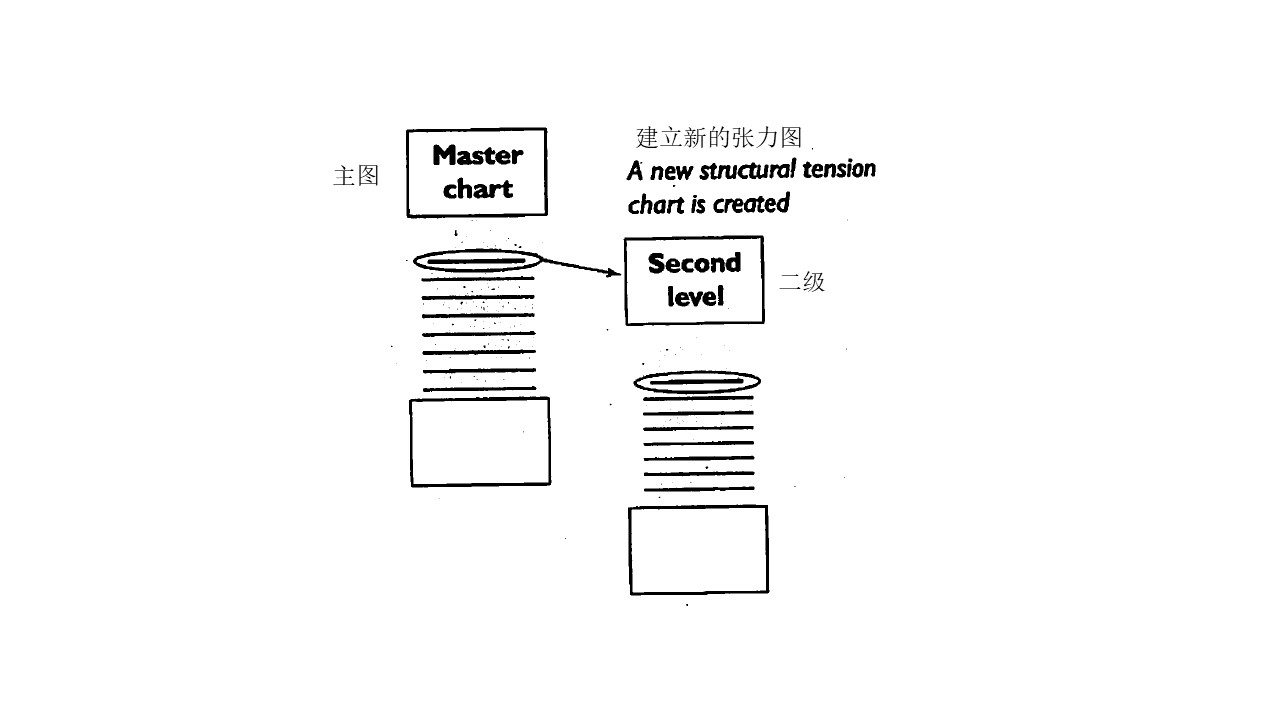
\includegraphics[width=10cm]{Fritz_diagrams_4.jpg}


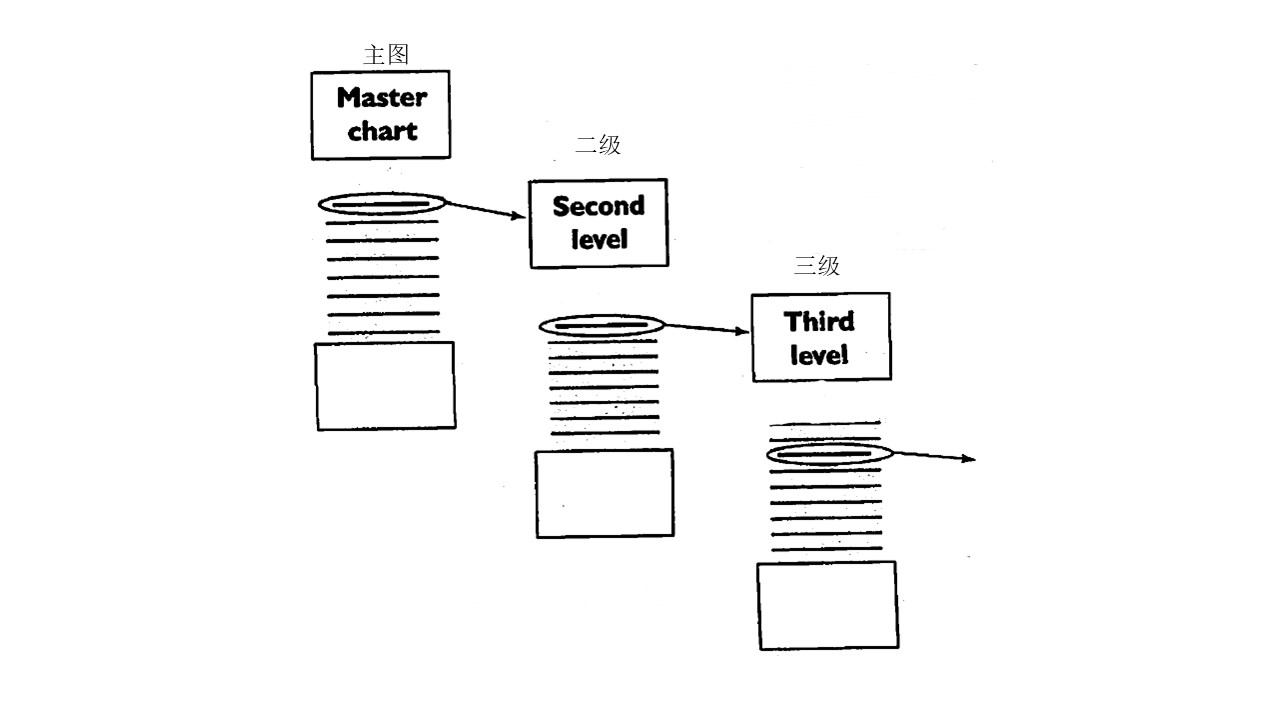
\includegraphics[width=10cm]{Fritz_diag5.jpg}


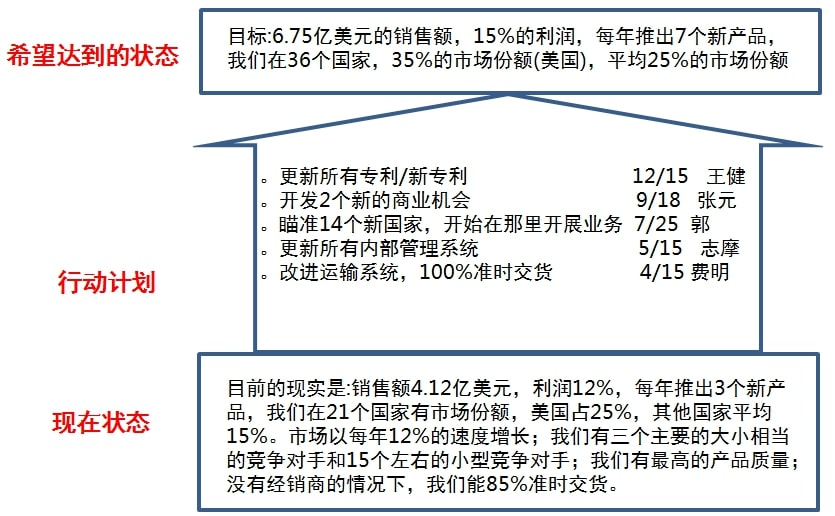
\includegraphics[width=10cm]{Drucker_4_tu3.jpg}

例如上图,高层希望提升销售额、利润,增加新产品等战略目标,必须要有开发团队的支持,如:控制交付后软件产品的质量,软件开发的生产率-每季度可以开发出多少新产品等,目标配合。

\hypertarget{ux5bf9ux8f6fux4ef6ux5f00ux53d1ux7684ux542fux53d1}{%
\subsection{对软件开发的启发}\label{ux5bf9ux8f6fux4ef6ux5f00ux53d1ux7684ux542fux53d1}}

可以用成熟度逐步完善,从基本(1)到可预测(3),让软件开发企业按部就班改善信息化管理:

\begin{enumerate}
\tightlist
\item
  基本项目管理
\item
  项目规模估算
\item
  分析项目历史数据建立基线(标杆)和预测模型
\end{enumerate}

\hypertarget{ux57faux672cux9879ux76eeux7ba1ux7406}{%
\subsubsection{1.基本项目管理}\label{ux57faux672cux9879ux76eeux7ba1ux7406}}

很多软件开发公司,缺乏基本项目管理系统 -\/-
包括项目工作任务分解,管理活动之间的依赖关系,记录在系统中,监控:实际与计划对比,是否延误或者工作量超支。

如果有这些信息,管理者便不用等到项目结束才知道项目是否有问题。

有开发经验的管理者会认为:``我每天都会跟开发团队接触,很清楚每个项目的进展与风险。不需要额外的信息系统帮我管理项目。''

也正是这个心态,妨碍了公司的健康发展,用刚才那个亲力亲为的管理模式,管理者管一百、两百开发人员勉强可以,但可以扩到五百六百已经很难。一千以上规模更不用想。但是反过来看,如果没有合理的信息系统,管理者凭什么去知道项目的风险,哪里会有重大问题?哪些项目质量不好?很可能等到客户投诉才得知。

\hypertarget{ux4eceux4f30ux7b97ux5f00ux59cb}{%
\subsubsection{2.从估算开始}\label{ux4eceux4f30ux7b97ux5f00ux59cb}}

估算缺乏依据,例如:很多项目经理只依赖个人经验估算项目工作量,以为项目的人天数就等同项目规模大小,不理解估算人天数时,已经假定了团队的生产率,所以应先估算项目规模,然后再依据团队生产率估算工作量。

如果要比较不同项目,必须依赖项目规模大小做归一
(Normalize),例如:我们不能用项目缺陷数来比较质量,必须用缺陷率(缺陷数/项目规模)。

在软件开发,如何估算项目规模一直是个挑战,大部分项目开始时无法知道详细需求,便很难用传统功能点分析来估算规模。
迭代项目可以在每个迭代采用简化功能点估算没迭代的规模,后面当需求更清晰时再更新总体功能点估算。(因大部分软件开发项目都采用敏捷迭代方式,不是传统瀑布式,大部分软件开发团队都可以用)

\framebox{%
\begin{minipage}[t]{0.97\columnwidth}\raggedright
功能点估算主要适合用于数据库、交易类软件开发项目,所以大部分软件开发项目都适用,也可参考行业数据基线作参考。

功能点数是一种估算项目大小的指标
(proxy),帮助我们估算项目的工作量进度、缺陷数等。

所以我们收集到项目数据后,需要分析这些项目参数是否与功能点数成线性关系,判断proxy是否确实能准确估算。\strut
\end{minipage}}

对于那些不可以用功能点的项目应如何估算?可以选择其他指标
(proxy),但也需要用项目数据验证。

\framebox{%
\begin{minipage}[t]{0.97\columnwidth}\raggedright
如果做一个全新项目,没有任何历史经验,第一两个迭代,只能依赖专家估算每一迭代的生产率与缺陷率。

但后面迭代的工作量与工期可利用前面迭代的实际数据来估算。

实例:\\
一个大客户希望在5个月内,对总共超过200个各类应用软件做``容器化''自动发布。
项目的总预算和工期已经固定。 乙方项目团队超过20人。
项目经理先与客户协商挑选一些''安全''的应用软件放在第二轮迭代先尝试。
(第一轮迭代,先做基础平台建设准备。)
这项目后面迭代(从第三轮开始到最后第六轮)的估算都会依据第二轮的生产率数据。
也从第二轮迭代经验,优化流程, 调高后面迭代的生产率系数。

虽然前面的迭代有超时, 项目最终还能按时完成。

这是偏实施的软件开发项目,传统功能点分析不适用,项目组采用传统代码行数为规模指标,从6轮的数据后,也验证代码行数确实可作为
proxy。\strut
\end{minipage}}

\hypertarget{ux57faux7ebfux6807ux6746ux548cux9884ux6d4bux6a21ux578b}{%
\subsubsection{3.基线(标杆)和预测模型}\label{ux57faux7ebfux6807ux6746ux548cux9884ux6d4bux6a21ux578b}}

\hypertarget{ux5229ux7528ux4fe1ux606fux5e2eux52a9ux51b3ux7b56}{%
\subsubsection{利用信息帮助决策}\label{ux5229ux7528ux4fe1ux606fux5e2eux52a9ux51b3ux7b56}}

没有数据就无法比较。

\framebox{%
\begin{minipage}[t]{0.97\columnwidth}\raggedright
有一次问一位下面有5位开发人员的开发组长,问他如何判断开发人员的学习进展,能力是否有提升?

他说:``我们每月都会有考核,多项打分(1-10分),我会每人在这期间是否完成下发给他的任务是否按时完成等打分。''

但他做判断时能否客观?比如下面小李开始时某方面表现较出众,很可能他其他项都普遍高分;反过来小王可能沟通表达能力较弱,会影响其他项打分不高,这是靠人主观判断的常见的误区。但如企业有收集每个开发人员的每周有效代码数、功能点数
(生产率)和一次性通过率(质量)等客观指标,考核便能比较客观,也能让个人和团队实时知道是否有改进。\strut
\end{minipage}}

好比锻炼跑步,目标想跑马拉松。
如果一直都没有收集跑步的数据,肯定很难有任何提升。
软件开发也一样,第一个挑战是如何让个人与团队开始有定期一两周收集数据的习惯。
开发工程师都是公司核心骨干,很有自己的想法。
必须让他们觉得数据有用,才愿意去做。
所以,我们会用一些互动练习,模拟项目组冲刺后做回顾。
让他们感受感受到有数据,并形成柱状图,趋势图等的讨论,比以前但依赖每人发表意见讨论更有效。

这种以数据监控团队效率/服务的管理方式,其实已经一直在很多服务业使用(如呼叫中心,每个团队的头顶都会有数字大屏,实时反映这个团队的平均解决客户问题时间,客户投诉率等。)也正是有了这些客观数据,才能激励团队想尽办法改进团队的成绩,不能比其他团队差。

信息只是一个工具,更关键的是背后的概念和业务本身,如果有了这些新的数据信息,是否可以帮我们更好做业务才是最关键。

软件开发的度量不仅仅能帮助团队和个人持续改进,也能帮管理者做决策。

例如软件项目报价。有一家公司各省的都有分公司,分公司主要谈业务接单,总部做开发。为了抢单,业务员都会尽量把压低软件价格,导致还未开工,项目经理就已经知道无法在预算内完成。

如果有收集以往同类项目历史数据,项目经理就可以估算项目工作量。请注意,我们没有说项目的报价,就是完全按照系统历史数据估算,业务变化万千,可能是战略需要,亏本也要接这个单,因为他可能会开拓后面附加业务。但有了这个历史数据的项目估算信息,管理者便可估计项目会亏多少,不会等到接单后才知道。

如果企业有不断收集项目数据,形成标杆,不断更新基线,企业便可以利用基线或者标杆去帮助知识工作者持续改进。

项目信息不仅仅是把项目管理从六十分提高到八十分,而是企业的最基本竞争力。刚才这个例子也可以扩大,不仅仅是用于一些投标客户定制化开发项目。如果公司是做软件产品也一样:
如何定产品的卖价,以前都是一门``艺术'',只有CEO或业务经理才知道,他也说不出来按怎么去定价,反正公司就活下来。但是如果我们有了那些项目的信息知道我们平均开发一个新的功能点要多少开发成本,对产品经理是很重要的信息,如何定软件产品的卖价的考虑因素。

正如德鲁克先生在九十年代的观点,就算你是一个传统的经理人,生意人主要是关注买卖,低价买入,高价卖出,要盈利。你可以想象量化管理如果做好,也可以帮到你。更深入去想,这个内部管理的信息化是一个很重要的企业竞争力。只是现在你的同行大部分都在睡梦中没有醒过来,当你发现他们醒过来才反应的时候,可能已经为时而晚了。

你可能会说:``你说这些都正确,但是我们还没到这个地步,暂时不需要像你说的那种推行量化管理。''\\
软件开发人员常会有一个误解:``我们跟那些大企业不一样。我们是无法像这种用数据做估算和计划,因软件开发变数太多。''\\

\hypertarget{ux5e94ux5982ux4f55ux5f00ux59cb}{%
\subsubsection{应如何开始}\label{ux5e94ux5982ux4f55ux5f00ux59cb}}

了解为何要度量? 改进目标?
为了让团队认同度量的重要性,我们会先把企业所有干系人聚在一起,开2天半的工作坊,辅导他们讨论公司战略目标,有哪些改进方向?如何利用数据做回顾,根因分析,让每个团队一起定度量计划,为了满足公司的发展需要,如何收集哪些数据,哪些因素会影响团队的质量与生产率?例如,如觉得代码质量可能是主因,要收集哪些指标来衡量代码质量?经过工作坊过后,我们会按生产率与质量两目标,做2天针对性地培训,教他们如何从需求可以估算功能点数、工作量,辅导他们利用数据模板,开始每2周收集项目信息。

我们4年前开始辅导团队如何使用简化功能点方式估算迭代的规模。我们的客户都能经过两天培训后便开始使用这方法开始收集项目迭代生产率数据。

建立基线\\
当企业团队、软件开发团队一直有收集以上的基本数据,我们就发现它们之间都有一个相对稳定的比例。有些可能会跟不同的客户方的业务有差异,例如你做一个高端的银行系统,可能跟一个普通的网购项目有差异,但是我会依据这些基本的差异把基线细分。我们就可以知道你是这类项目,从历史数据按现在需求估出来的项目规模,刚才说的成本进度、代码行数大概多少?我们没有说他非常精确,但起码它会比你单靠个人经验,拍脑袋估算更有参考价值。

\framebox{%
\begin{minipage}[t]{0.97\columnwidth}\raggedright
问:
增加了这么多数据度量和文档准备是否会增加额外的工作导致整体效率降低?
答:所以我们只收集关心的和用来分析的数据;例如我们一个迭代收集的数据都不超过15个,都是最基本的。如企业觉得不够,才增加。\strut
\end{minipage}}

``你是否要很高深的统计学概率等基本知识才做得到?''

管理者/项目经理,其实只需要懂得如何利用这些统计分析的结果,改善项目管理,不需要量化统计学专家。现在科技发达,有很多现成的分析工具,如果企业能累积到充分和准确数据,分析不困难。

最困难是如何让知识工作者有动力/有兴趣收集数据。
与制造业不一样,数据必须要由知识工作者提供。
如果他们不觉得提供这些数据对工作有帮助, 他们肯定不愿意。

就算公司规定,
如果他们不相信度量这些有用,他们很可能随便填报,公司也没办法。
所以数据是否被使用帮助团队做改进非常重要。

如果没有数据,冲刺后的团队回顾,大家都利用分析本冲刺的数据,如缺陷数分布,源于以往历史数据比较。
一起讨论找出根本原因在上一个从此采取改进行动,每个团队成员很自然会积极提供数据。

反之,冲刺大会没有任何项目数据,只是大家坐在一起讨论头脑风暴。
冲刺回顾会逐渐会变成内部``批判会''失去动力参加回顾。

公司积累了一定数量的数据后,比如\textasciitilde{} 70 - 100 组数据。
便可以做统计分析,并建立公司基线 和 预测模型。
如果公司有做数据,挖掘,大数据等服务,其实数据分析的方式类似。
经理,过程改进组长和项目经理不须熟悉统计分析,但他需要知道如何利用这些数据分析结果,帮他们做好量化项目管理与根本原因分析。

度量计划很关键,因信息化管理必须收集合适的数据。例如,有些管理层只关注项目进度是否延期,但不监控项目的质量(各类缺陷密度)。只关注结果,不关注过程。如果开发的质量不理想,大量缺陷导致很多返工,项目的结果(进度偏差)肯定不会好到哪里?

企业要信息化管理,不是简单一两个月便能完成。
所以必须有一个项目计划,有里程碑才会有效果。
但每个项目组都特别忙,没时间,怎么办?
参加CMMI高成熟度评估,可以使企业有动力订立一个9到12月的改进计划,按部就班地推量化管理。

\hypertarget{ux603bux7ed3}{%
\section{总结}\label{ux603bux7ed3}}

21世纪整体的环境变化比上一个世纪更快速,企业为了不被最终淘汰,首先必须从信息管理入手,不能再依赖以往经验做决策和管理。\\
你对以上的问题都心里有数吗?如果不是,便应想想如何赶上。\\
软件开发企业的管理改革,与我们辅导开发团队做量化管理如出一辙,都必须基于数据。管理层除了要关注内部团队的效率与质量外,更要重视上面提到的信息。\\
推行企业的变革肯定有难度。首先管理者要不满意现在的度量与分析,才会有动力下定决心去改。因为要成功,肯定不会一步到位,必须经过很多轮的试点,然后调整,才最后有效果。所以高层的决心与支持是成功的必需条件。

下一篇
会从他的2002 文章``他们是人,非雇员They're Not Employees, they're
People`` 谈起,以TQM 系统总结。



\hypertarget{ux9644ux4ef6}{%
\section{附件}\label{ux9644ux4ef6}}

\hypertarget{ux4f5cux4e1aux6210ux672cux6cd5-activity-based-costing-abc}{%
\subsubsection{作业成本法 (Activity Based Costing
ABC)}\label{ux4f5cux4e1aux6210ux672cux6cd5-activity-based-costing-abc}}

生产业越来越多用新科技降低成本,如果还是传统的按使用了多少人时,或用了机器多少时间来计算和分配成本已不能反映真正成本。
如没有一个完善的成本会计方式,管理层是难以知道内部的真正成本,也很难去定产品的合适价位。\\
例如,产品1234,生产量不多。 占用生产机器的时间也短。
但因不能占用生产设备的所有时间。
每次生产都要花精力去准备,完成后也需要再调整,把设备恢复到生产其他产品配置。
另外产品5678,大量生产,占用生产设备的所有时间,所以不需要花精力去准备。
如果按传统会计按占用机器投产工时分摊,大部分的成本都会分到5678产品。
分配到1234产品的成本却很低,并不能反映真正的成本。

针对传统会计不能 合理分摊成本,生产业开始使用ABC:

首先要把识别每一种关键成本因素。
例如,准备生产设备;编写管理生产设备的软件程序;设备占用的地方面积:设备检查次数等。
然后收集实际数据。 花6到12个月时间做ABC对企业的价值包括:

\begin{itemize}
\tightlist
\item
  管理者更了解每个产品的实际成本,定项目产品价
\item
  了解哪些成本效益不高,要针对性完善
\end{itemize}

软件开发虽然没有产品生产这么复杂,但仍要合理分摊复用模块成本。
例如,越来越多公司,使用标准产品和复用模块来增高项目的生产率。
但应如何把复用产品的开发成本分摊到项目中?
例如,如果是按产品开发组的实际工作量计算成本,
销售会说"为什么你的成本这么高,是否你的开发效率低
为什么要我这个项目为你买单?"
所以不能单看工作量,要能真正反映的参数(例如,软件功能点数),
也需要有信息化系统,计算项目实际成本,管理层才可以看得出哪些部分效率低需要完善。

%\begin{description}
%\item[]
%\begin{description}
%\tightlist
%\item[]
%-\/-\/-===\textless{}\textless{}\textless{} END
%\textgreater{}\textgreater{}\textgreater{}===-\/-\/-
%\end{description}
%\end{description}

\cite{drucker1References1}
\cite{drucker1References2}
\cite{drucker1References3}


 %done
\chapter{再读德鲁克 从管理外包人员到全面质量管理} % Introduction chapter suppressed from the table of contents

\framebox{%
\begin{minipage}[t]{0.97\columnwidth}\raggedright
有一家电力行业的软件开发部,因为要控制全职员工的人数,所以很多开发人员都是以外包形式聘用,以下这个表是我们抽看的三个项目的数据,第一列是这个项目的功能点数,倒数第二列是项目的缺陷数。


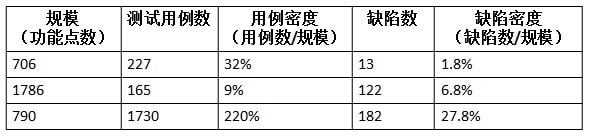
\includegraphics[width=8cm]{Druker_6_外包管理_1.jpg}

可以看出,项目的缺陷密度差异很大。与第一个项目团队沟通,发现写完代码没有单元测试,也没有评审代码,所以估计系统测试缺陷密度这么低,并不表示代码质量好,只是测试力度不够(项目1本来报给我的测试用例数是34,后来再说227才对)。\strut
\end{minipage}}

从以上的例子,就看到如果项目管理不善,质量问题可以很严重。

下面我们先回顾德鲁克先生2002年"They are not Employees,they are
people"文章{[}1{]}的重点,然后再探讨管理者如何提高知识工作者的质量与生产率。

\hypertarget{ux4e34ux65f6ux5de5temp-ux4e0e-ux4e13ux4e1aux96c7ux4e3bux7ec4ux7ec7}{%
\subsection{临时工(Temp) 与
专业雇主组织}\label{ux4e34ux65f6ux5de5temp-ux4e0e-ux4e13ux4e1aux96c7ux4e3bux7ec4ux7ec7}}

临时工(Temp)这行业早在50年代开始崛起,开始的时候主要负责一些简单岗位:文员、前台、电话操作员等,后来慢慢扩大到各种岗位,甚至总裁都有临时工。\\
\textbf{专业雇主组织 Professional employee organization (PEO)}\\
曾经,有顾问公司统计过一般公司管理员工的成本,约占总成本的25\%\textasciitilde{}30\%,所以如果有公司可以帮企业省去这部分成本,企业肯定愿意。这就是PEO公司的商业模式,它在90年代快速崛起,主要为客户提供企业管理人员,包括行政、人事等。\\
这两类公司为企业创造什么价值?为什么这么受欢迎?\\
德鲁克先生用一个小型医院为例:
一家有三百个病床规模的医院,大概有3000员工。其中有一半多是专业的知识工作者,除了医生、护士外、还有其他很多辅助角色:如物理治疗、化验、X光等专业岗位,但在这类医院里,每个专业可能只需要几位。医院的主管也不可能每个专业都懂,他如何管理手下各种专业人员呢?而且由于每个专业的人数不多,升迁的机会也几乎是零。例如,这医院的化验室专员全院只有三位,没有任何上升机会。但如果这些专业人员是受聘于PEO外包公司,有能力化验人员可能会被调到一些更大的医院去。而这些人也愿意用这种形式去服务医院。\\
这种现象也不仅仅适用于医院,一些百货公司、金融服务公司也常用这种方式,以获得专业性强的员工。所以这种无论临时工公司或者PEO公司,无论对员工或者雇主都有价值和吸引力。\\
这些Temp供应商 和 PEO
说能帮助企业管理员工,提升效率。你相信吗?让我们先听听大陆软件开发的管理者
和 临时工的 心声:

\hypertarget{ux5916ux5305ux95eeux9898}{%
\subsection{外包问题}\label{ux5916ux5305ux95eeux9898}}

\framebox{%
\begin{minipage}[t]{0.97\columnwidth}\raggedright
某北京IT总监的外包心得分享:\\
1. 外包的主因是降低风险\\
2. 用人员外包控制员工数量\\

\begin{itemize}
\tightlist
\item
  外包主要选我们没有它们的技术(外包公司可以提供此技术或产品或软件开发),一般考量是他们是否已做过\\
\item
  外包人员加入到我们的开发团队onsite人员,一起工作\\
\item
  问题主要是怎么调动人员积极性\\
\end{itemize}
\strut
\end{minipage}}

不少企业为了控制全职员工人数,会把软件开发项目外包出去。\\
但承包商人员水平与积极性难以保证,很可能导致软件质量出问题。\\
部分公司内IT员工的心声:\\
*\textbf{通过外包途径招聘人员的技能、质量不太能够符合项目要求,需要花费大量时间、精力去做培训,希望公司招聘外包人员时,考虑人员质量,解决项目实际人员需求。}\\
*\textbf{外包公司写的代码质量与我们自己写的相差甚远,也没有做单元测试,没有做静态代码检测,写完代码也没有做人工走查,导致我们后面很多返工。}\\
部分外包承包商员工的心声:\\
*\textbf{最大的问题是项目成就/责任感低,能少做的尽量不多做。因太多因素影响项目总体成败,我们(承包商)认为只要完成SOW里的内容就算项目成功。}\\
*\textbf{虽然公司经常组织学习甲方的产品,培训考试,项目质量主要由发包商项目经理(PM)控制,我们对项目质量关注度少,主要听PM安排。}\\
{[}SOW=Statement Of Work 可简单理解成项目需求范围 {]}\\

\hypertarget{ux77e5ux8bc6ux5de5ux4f5cux8005-ux4e0e-ux7cfbux7edf}{%
\subsection{知识工作者 与
系统}\label{ux77e5ux8bc6ux5de5ux4f5cux8005-ux4e0e-ux7cfbux7edf}}

``现代企业都依赖知识型团队, 比较50年前以劳工为主的企业,
更需要关注每一个员工的健康成长。 知识工作者最能为公司产生价值。
甚至企业的成败也依赖于知识工作者的表现。

企业不可能大量招聘卓越的人,所以管理者的挑战是如何使普通人做出超凡的事。好比杰出的指挥家能领导一普通乐团演奏出非凡的乐章。''\\
公司的创新大部分依赖于知识工作者,所以我们无论是用外包形式或者正常聘用,知识工作者是企业的核心资源(capital)。\\
以前的工业时代,是劳动者支撑系统制造产品,在当今的知识型社会恰恰相反,企业系统要支持知识工作者,让他们能发挥效益。

从外包人员的心声,和其产出软件的质量,都能觉得他们当中的很多人缺乏积极性。
所以不要以为单靠加强培训就会有效果。

具体有什么方法呢?

\framebox{%
\begin{minipage}[t]{0.97\columnwidth}\raggedright
一家工厂舍弃了传送带生产方式,学习丰田生产方式(Toyota Production System
TPS),权力下放给一线员工。企业总工有以下感想:\\

\texttt{..去巡视生产现场的时候,有一位女员工对我说:"以前每一次往生产线跟前一坐,我满脑子就都是怎么还不到5点呢?但现在上班成为一件让人高兴的事。"~听了她的话以后,我更加相信生产改革的方向没有走错。..}~\\
\strut
\end{minipage}}

为什么丰田生产方式这"系统"能改变生产现场员工的积极性?

\hypertarget{ux4e30ux7530ux6545ux4e8b}{%
\subsubsection{丰田故事}\label{ux4e30ux7530ux6545ux4e8b}}


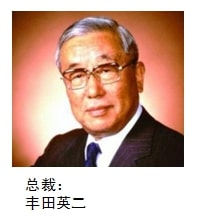
\includegraphics[width=8cm]{丰田总裁.jpg}


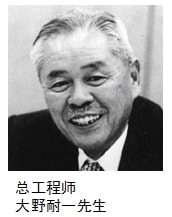
\includegraphics[width=8cm]{大野耐一.jpg}

二战后50年代,丰田汽车规模很小,经营很困难,在破产边缘。
但丰田英二先生明白美国批量生产线的弊端,意识到未来的汽车生产必须是Just-In-Time::

\begin{itemize}
\tightlist
\item
  每一辆都是按客人订单订制:例如,颜色,配置,左右钛等
\item
  从钢材原料开始,整个生产线,零等待,零浪费
\end{itemize}

\begin{description}
\item[]
\begin{description}
\tightlist
\item[]
每个工作步骤所需配件按生产需要到达
(不晚,也不早到),把生产过程中的配件降到零
\end{description}
\end{description}

安排总工大野耐一去美国汽车公司考察,
他从美国的超市(非汽车公司)得到如何做Just-In-Time的启发。
回国后就开始在丰田致力推动。


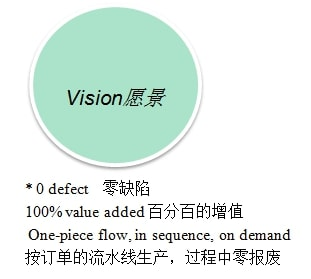
\includegraphics[width=10cm]{远景1.jpg}

开始时,很多人都觉得这个愿景好像是远不可及的梦想。今天Just-In-Time已成为汽车制造的主流,例如:日产在英国牛津(Oxfordshire)专门生产mini
车的 工厂便能做到:

\begin{itemize}
\tightlist
\item
  从钢材原料到生产出汽车只需要24小时
\item
  整个生产线没有任何中间等候,每68秒出一辆
\item
  每天生产1000辆车
\end{itemize}

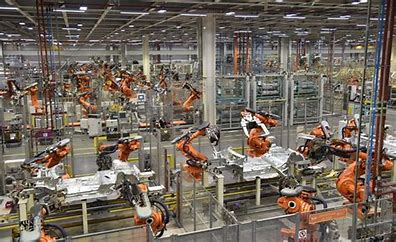
\includegraphics[width=10cm]{NissanRobots-OIP_h8UAC7FBjlaCmA_mBepJjQHaEi.jpg}

\textbf{挑战}:每一辆汽车都不同 -- 颜色,设备,左右驾驶座等

\begin{itemize}
\tightlist
\item
  生产线上每一辆汽车都按照客户需求订制
\item
  组件不早不晚按需求准时到达生产线
\item
  这便需要信息化系统把客户订单转换成生产信息
\end{itemize}


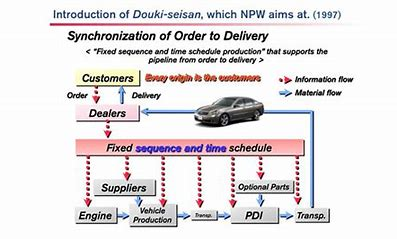
\includegraphics[width=10cm]{NissanJIT_OIP_RQGKy67DWGTu-DQiOCqW2gHaEK.jpg}
例如,生产线上每一辆的颜色都可以不同:\\

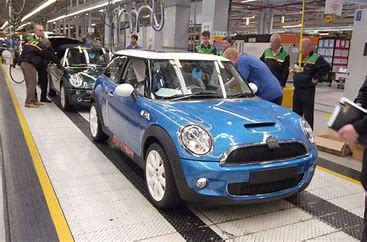
\includegraphics[width=10cm]{NissanProdLineOIP_wJFmfMl7q2_V8JaQi4kQ8QHaE6.jpg}\\


\hypertarget{ux7ba1ux7406ux5916ux5305ux4ebaux5458ux7684ux6311ux6218}{%
\subsection{管理外包人员的挑战}\label{ux7ba1ux7406ux5916ux5305ux4ebaux5458ux7684ux6311ux6218}}



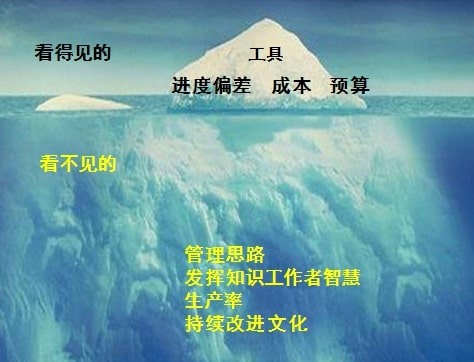
\includegraphics[width=10cm]{冰山.jpg}

\textbf{问}:我们不是讨论如何管理软件开发外包人员吗?为什么转到讨论丰田生产方式?
我们都不是生产业,有什么关系?\\
\textbf{答}:德鲁克先生2002年的文章强调:不能依赖外包公司帮你管理,
还是必须靠管理者自己。

很多软件开发公司缺乏相关度量。
例如,只管项目有没有延误,客户有没有投诉等水面上看得见的东西;但不知道生产率(每人每天生多少功能点)/现在是什么水平等水面以下看不见的情况。
没有度量就无法谈改进,无法管理。

管理者也不能仅看表面的数据,如项目延误,成本是否超支,更需要看过程中知识工作者的生产率和质量是否有提升。

外包人员每天工作都是被动地应付客户的投诉;
只想被安排的任务不延误,不会想怎样提升整个开发的效率与质量。
工作自然没有动力。

反过来,如果大家都知道自己的生产率水平, 像丰田有具体的阶段改进目标。
管理者辅导团队如何利用智慧,找出问题的根因,实施应对措施,看能否达到预期提高(而不是靠喊`要努力,努力')。
公司便可以生产出更多新产品,使客户满意,增加收入,
公司根据各团队贡献,鼓励团队分享成果,形成持续改进(PDCA)良性循环。

有这类``系统''才能根治外包人员的管理问题。

为什么丰田能成功地把汽车生产做到 Just-In-Time
,超越西方的巨头,使日本汽车制造过程成为世界"标准"?
但我们不能单从表面看这"系统"的方法和技巧,例如大家都熟悉的看板管理(他的竞争对手通用、福特、肯定都学过),所以更重要是了解背后的管理思路:\\

\hypertarget{ux4ee5ux5fd9ux788cux4e3aux803b}{%
\subsubsection{以忙碌为耻}\label{ux4ee5ux5fd9ux788cux4e3aux803b}}

\begin{itemize}
\tightlist
\item
  不吝惜智慧,但要吝惜汗水
\end{itemize}

\framebox{%
\begin{minipage}[t]{0.97\columnwidth}\raggedright
{把``动作''转变为 ``工作''}
以前,当大家批评某机关的工资太高时,职员会以上班时间很长,
``一直在努力工作''为由来反驳人们的批评。这其实是一种对于``有动作''和``在工作''的混淆。不管上班时间有多长,如果没能够创造出利润,那么就不能称之为工作,也不能称之为一直在努力。
丰田是把``动作''和``工作''分开考虑的。\\
strut 在丰田看来,
``就算一直在动也不代表那个人在工作''。
省掉徒劳动作,把``在动着''转化为``在工作''。\\
大野耐一先生曾经问过年轻员工:
``每天工作一小时左右,你们能做到吗?"
听了这句话后,有人抱怨``算上加班时间,我们一天工作九个小时,他那句话是什么意思?"确实,他们在公司待了很长时间,但如果把``有动作''和``在工作''分开考虑,九个小时中,真正在工作的时间可能只有一小时。大野先生指的是这一点。\\
关键的不在于流着汗在公司转了多长时间,而要把自己的工作区分成``徒劳作业''和``有价值作业''。\\
\strut
\end{minipage}}

因缺乏数据,很难判断这些软件开发人员每天有效生产多少?什么因素妨碍员工生产率提升?\\

\framebox{%
\begin{minipage}[t]{0.97\columnwidth}\raggedright
二战后,日本经济萎缩,丰田辞退了不少员工;1950年,朝鲜战争,需要大量增产,但丰田选择了只增加设备,而不增加人手,大野先生也借这机会,完善丰田生产方式,成功找到了以不增加人手为前提的增产办法。
\strut
\end{minipage}}

在软件开发行业,跟当年丰田一样,也会因市场的起落导致景气或不景气。很多公司预计到项目量增加就立马增聘开发、测试人手,而不是基于现有人力,如何更好利用自动化来提高生产率。我们看很多公司也是因为测试团队天天都说人手不够,增聘测试人员,反而妨碍了公司推动测试自动化。\\

\hypertarget{ux57f9ux517bux4ebaux624d---ux903cux4ed6ux4eecux52a8ux8111ux7b4b}{%
\subsubsection{培养人才 -
逼他们动脑筋}\label{ux57f9ux517bux4ebaux624d---ux903cux4ed6ux4eecux52a8ux8111ux7b4b}}

\framebox{%
\begin{minipage}[t]{0.97\columnwidth}\raggedright{人了不起的智慧}
所谓丰田生产方式其实就是要建立起一种体制,把``人了不起的智慧''引导出来,使得这些智慧能在生产一线得到充分发挥。所以说``丰田生产方式源自人的智慧''。\strut
\end{minipage}}

企业相信员工的智慧以后,员工们的干劲、使命感、责任感都会随之而生,最重要的是,员工们会因此逐渐对工作抱有自豪感。一旦员工们的意识改变了,理所当然地,企业的竞争力也将获得很大的提高。\\
丰田生产方式是TQM (Total Quality
Management全面质量管理)的最佳例子,TQM强调专注客户、持续改进、以数据说话、员工参与等,丰田生产方式覆盖了
TQM 原则的 七项 (除了战略)


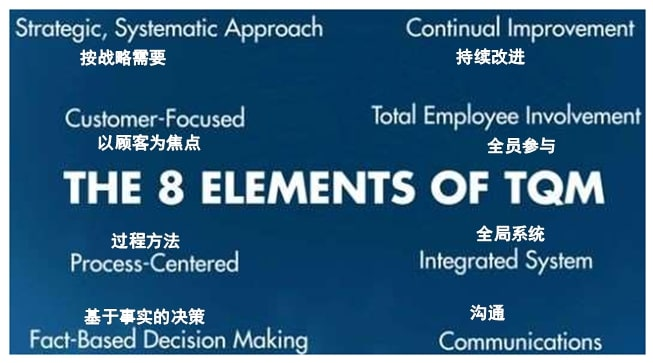
\includegraphics[width=10cm]{TQM_1_2.jpg}

\hypertarget{ux4eceux5fc3ux91ccux76f8ux4fe1ux5927ux5bb6ux7684ux529bux91cf}{%
\subsubsection{从心里相信``大家的力量''}\label{ux4eceux5fc3ux91ccux76f8ux4fe1ux5927ux5bb6ux7684ux529bux91cf}}

\begin{itemize}
\tightlist
\item
  不是靠``一个不平凡的人'',而是依靠``一百个平凡人''来创造亮眼的成绩
\item
  生产产品就是培养人才
\end{itemize}

\begin{description}
\tightlist
\item[]
``做事业最关键是人.......`培养人才'为基础''总裁丰田英二先生
\end{description}

\begin{description}
\tightlist
\item[]
有一位丰田员工被问到``丰田生产方式到底是什么''的时候,这样回答:
``就是在人的智慧建起的基础上,立起了自动化和及时生产这两根支柱。''\\

\textbf{他所说的``人的智慧''是指``在一线工作人员的智慧''}。\\
\end{description}

\hypertarget{ux4e0dux4ee5ux6211ux4eecux516cux53f8ux4f5cux4e3bux8bed}{%
\subsubsection{不以``我们公司''作主语}\label{ux4e0dux4ee5ux6211ux4eecux516cux53f8ux4f5cux4e3bux8bed}}

\begin{itemize}
\tightlist
\item
  不是从``专业''的角度,而是从``顾客''的角度生产产品
\end{itemize}

\begin{description}
\tightlist
\item[]
创业大忌 -
闭门造车,所以丰田的原则,对客户有用就一定做出来,但对客户无用,或者不想要,就绝不生产。\\
\end{description}


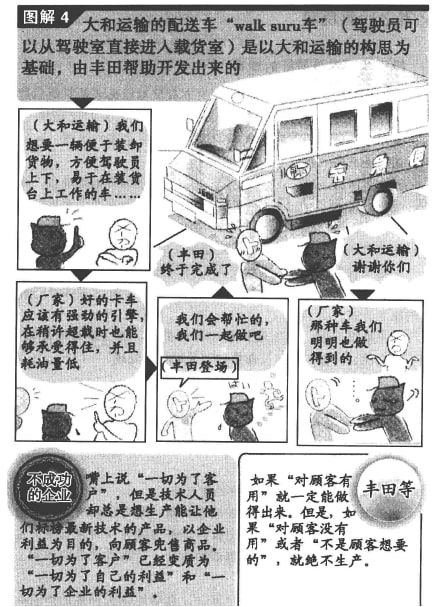
\includegraphics[width=10cm]{丰田p3.jpg}

很多软件公司现在已经开始从以前的瀑布式开发(几个月后才有产品出来),变成敏捷冲刺,每2周便与客户回顾,看是否是他们要的东西。我们QAD的方式基于SCRUM的基础上,也要求客户把需求分成``实体''与``行为''写需求,自动计算功能点数,也帮助开发人员减少误解客户需求。

\hypertarget{ux6807ux6746ux7ba1ux7406-benchmarking}{%
\subsubsection{标杆管理
(Benchmarking)}\label{ux6807ux6746ux7ba1ux7406-benchmarking}}

丰田(如下图)很注重各种标杆,例如内部标杆、竞争性标杆等。软件开发也应该同样利用数据来制定量化目标,例如生产率。最近行业也要求做功能点估算来统一软件报价,有了功能点,团队就可以利用它来衡量软件团队的生产率,它也有不同行业的标杆做参考。


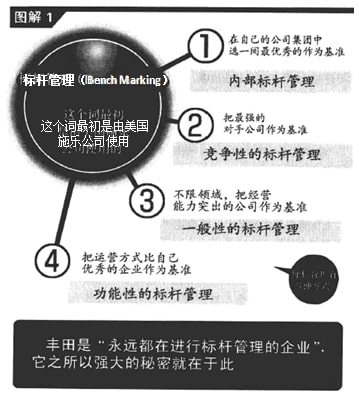
\includegraphics[width=10cm]{丰田p1.jpg}

\textbf{收集每迭代项目数据,建立标杆}\\
我们要求每个迭代项目组都需要提供数据,填进模板中,开始时因公司还没有历史数据的基线,我们就借用行业数据,从下图看到C\#编码的有效率都是很好(绿色)


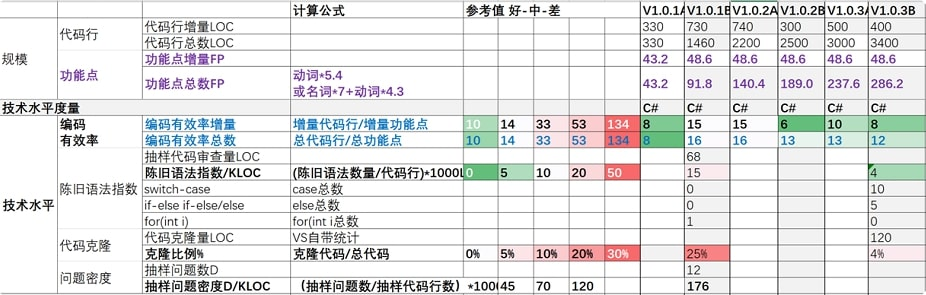
\includegraphics[width=10cm]{陈爱明p15.jpg}

因各项目的数据都会汇总在一个公司级的数据表,每个项目组不仅仅看到自己的表现,也可以看到其他项目组的情况。

建立公司标杆不能单靠数据分析员一个人分析判断,而是应由过程改进组与所有相关项目经理一起讨论:\\
*展示(投影)项目多轮迭代数据

\begin{itemize}
\tightlist
\item
  这些不同项目的数据类似吗?还是差异大,要分开定基线?
\item
  里面有些离散点数据?为什么?
\item
  数据准不准确?合不合理?
\end{itemize}

这样才可以知道数据是否正确,标杆/基线是否适用于项目?

\hypertarget{ux5bb9ux6613ux5b9eux73b0ux7684ux76eeux6807ux4e0dux662fux597dux76eeux6807}{%
\subsubsection{容易实现的目标不是好目标}\label{ux5bb9ux6613ux5b9eux73b0ux7684ux76eeux6807ux4e0dux662fux597dux76eeux6807}}

\begin{itemize}
\tightlist
\item
  不是``削减一成'',而是通过``取消一个零''来发现浪费
\end{itemize}

把原先需要三小时的工作,改用三分钟完成。\\
听到上司这个要求,你该怎么回答呢?多数人会常识性地回答:``这太强人所难了''、``绝对做不到''。\\

\framebox{%
\begin{minipage}[t]{0.97\columnwidth}\raggedright
丰田 {``单分换模(Single Minute Exchange of
Die)''}例子:\\
1965年,丰田汽车在推行丰田生产方式时遭遇一个瓶颈:装置更换时间太长,其中特别是500吨冲压机和1000吨冲压机的模具,更换时间长达2\textasciitilde{}4小时。如果不缩短这两个模具的更换时间,就不可能实现多品种少量生产方式。
\\挑战由大野耐一先生统领,在生产管理的先行者,新乡重夫先生的指导下,分两个阶段展开。\\
改善开始之前,新乡先生凭借自己多年的工作经验,了解到装置更换有两种方式。\\
①内部装置更换------必须在机器停下来以后,才能进行的装置更换。\\
②外部装置更换------能在机器运转过程中,或是在运转起来以后,进行的装置更换。\\
要缩短时间,把内部装置更换和外部装置更换清楚地分开来是一个关键。能在外部装置替换作业中进行的工作,就全部在外部装置替换过程中实施。同时,分别对内部装置替换和外部装置替换进行改善。通过这种方法,装置更换时间缩短为一个半小时。\\
完成这一改善花费了半年时间。通常能有这样的成果就可以告一段落了。但是,大野先生仍要求进一步缩短时间。\\
他要求把更换过程``缩短为3分钟!''通常通过改善能把原先的2\textasciitilde{}4小时缩短为一个半小时,就可以很满意地说``已经很好了''。但是,大野先生不这么想。\\
他认为:``既然能缩短到这个水平,那么继续改善肯定可以把时间缩短为3分钟。''\\
改变汽车生产的单分换模的秘密\\
对于这一要求,在以新乡先生为中心的技术小组中,自然有人提出``3分钟绝对干不完''。但是,新乡先生认为:``如果能把内部装置更换全部转化为外部装置更换,3分钟也不是不可能\\
之后,他着手对多达100个以上的项目进行了改善。\\
首先,进一步对内部装置更换和外部装置更换进行细分,彻底把内部装置更换转化为外部装置更换。同时,想方设法对各种切割工具和模具进行设置,使得更换时用一个动作即可完成。此外,在紧固件上也动了很多脑筋。这样,终于创造出了无数项不花时间、能够简单完成同时可以在作业时保持稳定的改善。\\
紧接着,对作业顺序反复进行改善,实施标准化(制定没有多余工序的作业标准)。这样,在挑战进行了三个月后的某一天,真的只要3分钟就能完成了!这个结果让所有人都大吃一惊。\strut
\end{minipage}}

看下面两个软件项目实例:

\framebox{%
\begin{minipage}[t]{0.97\columnwidth}\raggedright
项目是要更新信息基础平台,团队一直很注重配置管理和模块化设计,为了避免对生产的影响,先做好策划与准备。到了更新时,2位工程师准备新的基线,先本地测好,也准备完整的验收测试包,测试暴露了一些缺陷,先把主要的问题解决,与开发团队讨论后,一致同意进行更新上线。整个更新的过程包括跑完所有自动化测试,在1天内完成。\strut
\end{minipage}}

\framebox{%
\begin{minipage}[t]{0.97\columnwidth}\raggedright
另一个项目是要对一个老系统做修复,这系统已经投产了很多年,希望更新应用服务器的版本。(因为系统本来应用服务器的版本厂家不支持)这个项目最后占用了6个人2个月才能测试好,完成,进入投产。\strut
\end{minipage}}

虽然以上两个项目不是完全一样,但可以看到如果动脑筋,策划好,也能``取消一个零''。\\
例如,我们去年有敏捷团队可以经过6轮冲刺(3个月)把系统缺陷密度减半。

\hypertarget{ux6839ux56e0ux5206ux6790}{%
\subsubsection{根因分析}\label{ux6839ux56e0ux5206ux6790}}

(五个为什么 是一种找根因的方法 , 详见附件B)

\begin{itemize}
\tightlist
\item
  不停留在``原因''上,而要找出``真因'',彻底改善
\item
  不追究责任,而是追究原因\\
\end{itemize}

丰田的大野耐一先生说:

\begin{description}
\tightlist
\item[]
\emph{做到一半是不行的,只有一个期限,``到完成为止''}
\end{description}

当工程师报了有问题就必须要求工程师查找原因、提供数据,但很多时候这个工作并不简单,但大野耐一先生决不放弃,必须找到根因。

我们辅导量化敏捷开发, 每迭代回顾都要收集数据,并做根因分析:
在软件开发,当遗漏到系统测试的缺陷多,便要做讨论,探讨是什么原因?例如:是开发质量问题或测试力度不够,开发的编码有不良习惯,例如拷贝代码,用很大的类等(详见附件A"软件开发质量")。针对代码质量问题,团队便做培训,用新的方式看看会不会有改善?

同样,本来自动化测试的效率在头2、3个迭代都是比较弱(粉红)的,我们与测试人员探讨自动化测试脚本的不足,并针对改善后,后面的迭代就有显著改善(绿)。


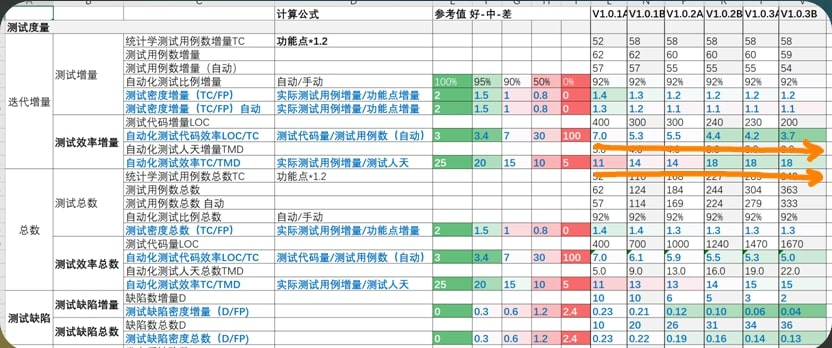
\includegraphics[width=10cm]{陈爱明p17.jpg}

\textbf{预防同类问题再发生}\\
有一家专门做电力的软件公司,它为了加快发布的频率,已经在2年前开始做到每2周自动发布,但他们还是很关注发布的质量,所以发布前都有多轮的审批,确保质量,才允许发布。

如果项目经理赶不上某次发布的,他们就会走一个失效分析
(FMEA),回顾整个过程,哪步出问题?背后什么原因?如何避免同样的问题以后发生。

\hypertarget{ux6210ux957fux6bd4ux6210ux529fux66f4ux91cdux8981}{%
\subsubsection{成长比成功更重要}\label{ux6210ux957fux6bd4ux6210ux529fux66f4ux91cdux8981}}

\begin{itemize}
\tightlist
\item
  要培养人才,``改变体制''比``改变人''更有效
\end{itemize}

有些工厂只依赖张贴标语、海报,希望可以减少工地的事故发生率,但丰田不注重喊口号,而是动手干实事,包括机械保安、设备保安等


\includegraphics[width=10cm]{ft_223_1.jpg}

\framebox{%
\begin{minipage}[t]{0.97\columnwidth}\raggedright
{叫人做之前自己先做一遍给他们看}
本田技研工业在中国创立广州本田的时候,派往当地的都是即将退休的经验丰富的中高年龄层技术人员,这批技术人员成为了厂里的中坚力量。正因为他们的努力,广州的本田工程才获得了成功。\strut
\end{minipage}}

软件开发如何确保质量?比如一个团队有些新人,绝不能简单分派任务,让他自己随意写代码,组长要先想好整个架构,主要有哪些类,之间有什么关系,每个方法和类要注释说明,然后分配给新手去执行,避免事后返工。学校里编码练习也不会只描述需求,通常会指出需要那些类、方法,有什么作用,防止学生走偏。

但软件开发人员的能力有高低之别,如何让新手可以跟高手有效学习呢?代码评审其实是很有效的培训,比单靠讲课更有效。我们会建议团队按高手的时间来安排评审,让新手从中学习。不一定预定在哪天哪时,以便减少对高手时间安排的影响(他时间宝贵),也能取得培训效果。

\hypertarget{ux6240ux6709ux4ebaux53c2ux4e0eux6539ux8fdb}{%
\subsubsection{所有人参与改进}\label{ux6240ux6709ux4ebaux53c2ux4e0eux6539ux8fdb}}

\framebox{%
\begin{minipage}[t]{0.97\columnwidth}\raggedright
{带诚意去赢得协作}
B先生所在的A公司曾以丰田生产方式为基础进行了生产改革。\\
要进行生产改革没有技术部门的配合是行不通的。但是,任凭
B先生怎么要求,技术部门依然毫不合作。B先生实在没有办法了,只能向总裁要求:
``请加大我手上的权力,让我可以支配技术部。''总裁回答:
``你去给我请教了大野(耐一)先生以后再说!''\\
于是B先生去找大野先生,在听他诉说了自己面临的窘境以后,大野先生对他说:
``你这一两天跟我一起去工厂转转吧!''并于百忙之中抽出时间带B先生参观了丰田的工厂以及附近的协作企业的工厂。这期间,大野先生什么话都没说,只在第二天下午问B先生:``怎么样,你明白了吗?''\\
B先生回答:
``我觉得在工厂听到的关于厂长的改善事例,跟丰田方式所强调的重点好像不太一致。''听了B先生的回答以后,大野先生点头:
``就连我,也是一直都在忍耐的啊。工作并不是有权力就能解决问题的。要想得到对方的理解和信任,拿出诚意去找人家吧。''\\
从那以后,
B先生再也不找``因为我手里没有权力''之类的借口,而总是带着诚意去找对方协商,不久以后,他成功地对A公司实施了生产改革。\\
每当听到有人感慨``下属不听话''的时候,一位曾在丰田工作的人就会说:
``你要求自己的孩子"每天学习三小时'时,他会听话去学习吗?''\\
对方的回答是:
``估计没用。''\\
``连自己的孩子都这样,更何况那些成年的员工呢?''\strut
\end{minipage}}

我们开始要求企业拿出试点项目来做量化敏捷开发(QAD)时,阻力也很大,我们只好挑一些愿意并有能力的先锋团队。过了几个月后,其他本来观望的项目组看到确实有效,也愿意加入。所以在公司推动过程改进必须先试点后推广。

因为与以往的做法截然不同,必须经历:\\
学习 - 尝试 - 学习 - 尝试执行\\
不断循环才开始把握。 团队也会问老师收集了几轮数据了。不知道有什么用处?
但我们不直接给答案,而是重新提醒他们各种学过的分析技巧与方法,让他们自己尝试找答案。

反过来,如果团队没有经历这个过程,只遵循老师制定的一套固定方法,项目组很可能评估过后,便恢复以前,不能持续。

推动量化敏捷开发也一样,不能单依赖一套固定方法,我们利用CMMI量化管理的实践重点,例如量化目标、度量可操作定义、基线预测模型等。首先教他们用简化功能点,使每个团队都有可比的规模大小基数,然后让他们收集每一迭代的缺陷数,工作量和一些可控因素,引导他们如何分析这些迭代数据,制定本项目的下一迭代的量化目标。
虽然我们会提供一些统计分析的技巧,给他们参考,但是还靠项目经理与团队自己讨论,看用什么方式达到量化项目管理的要求。

\hypertarget{ux603bux7ed3}{%
\section{总结}\label{ux603bux7ed3}}

这3篇"再读德鲁克",从信息化挑战开始,我们探讨管理者应如何做好数字化、智能化管理,收集哪些数据,帮助企业管理。然后我们再回顾有哪些方法,可以帮助知识工作者提高效率和质量。这篇我们从管理外包的问题开始,引申到丰田生产方式的一些案例,了解管理者的"系统"。

丰田故事让我们看到``系统''如何帮公司培养知识工作者,发挥人的无限智慧,
为公司增值。\\
汽车制造大部分利用自动化机器,但当今软件开发生产和质量,
非常依赖开发人员的水平, 所以我们更需要建立``系统'',帮助员工快速成长。

前面分享的九个丰田管理思路,其实都能在软件产品开发用上:

\begin{enumerate}
\tightlist
\item
  以忙碌为耻
\item
  培养人才 - 逼他们动脑筋
\item
  从心里相信``大家的力量''
\item
  不以``我们公司''作主语
\item
  标杆管理 (Benchmarking)
\item
  容易实现的目标不是好目标
\item
  根因分析
\item
  成长比成功更重要
\item
  所有人参与改进
\end{enumerate}

在互联网年代,数字化管理已经不是未来,在软件产品开发,很多公司已经从以往的瀑布型开发模式转为敏捷开发,以便更好反应客户的需求变化,也让团队效率提升到极限。

2周一冲刺比以往几个月才完成一个项目,本应可以收集十倍的数据(假如项目平均5个月),但碍于敏捷方法缺乏一套度量标准,公司无法形成基线
/ 标杆。

4年前,我们开始为企业推动量化敏捷开发(QAD),团队就可以基于功能点的生产率与质量基线,并在6
- 9个月时间,利用对可控因子的根因分析,可以把缺陷率减半。

从我们过去三年,针对那些已经使用敏捷SCRUM开发的软件开发公司,辅导团队提升到量化敏捷开发,
但管理层千万不要以为这个改变过程轻松、 快速。正好相反,
任何文化的改变都会遇到很大阻力,但只要管理深信必需建立这个``系统'',破釜沉舟,才有希望成为大陆软件开发未来的``丰田''!

\hypertarget{ux53cdux9988}{%
\section{反馈}\label{ux53cdux9988}}

\framebox{%
\begin{minipage}[t]{0.97\columnwidth}\raggedright
上海一总监问: "可否说明一下市面流行的敏捷开发(如 SCRUM ) , 如何分配任务
, 有那些方法?"\strut
\end{minipage}}

敏捷一般建议基于I.N.V.E.S.T.原则把需求分解成用户故事。

\begin{description}
\tightlist
\item[]
Independent (from other user stories)

Negotiable (on how to implement)

Valuable (for customers)

Estimable

Small (to complete in a Sprint)

Testable
\end{description}

但具体怎么分每个人可能有不同的想法,而且用故事点 估计规模大小,
但故事点只是项目组自己的定义,不同团队间无法比较,难以利用各项目度量数据,建立公司标杆(基线)。

针对以上不足, 也方便开发/测试能与需求打通,
和团队使用功能点作为规模,估算工作量 / 工期。

我们会教团队按场景(Scenario) 、 实体(Entity) ,行为(Activity)写需求。
以便与开发工作 / 测试工作对应。\\
(实例 ,注: 实体浅蓝色,有框)


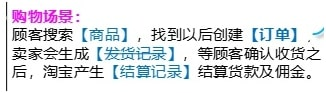
\includegraphics[width=10cm]{场景1.jpg}

团队便容易把与行为对应的开发任务,按优先级,安排到各冲刺中。
测试人员也可以从而估算出测试用例数,测试工作量,甚至缺陷数范围。
敏捷团队从定性管理,升到定量管理。


\cite{drucker3References1}
\cite{drucker3References2}



 
\chapter[敏捷开发]{再读XY理论:如何支持敏捷开发}

培训一开始,我把3天的范围、敏捷的主要概念讲完后,立即在白板左右两面写上一些数据,让学员猜它们分别是美国西岸哪两家科网公司?

``大家猜一下,下面两家都是美国西岸的公司分别是什么公司?''\\
我在敏捷ACP 培训,通常都会用这个问题开头。\\

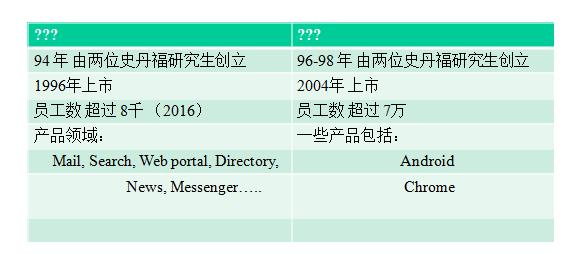
\includegraphics[width=10cm]{0A_Agile_stories_p4.jpg}

他们立即猜到左面是 YAHOO! , 右面是Google 。\\
2000年,谷歌还是小公司,雅虎是已经是大规模的上市公司,但现在大部分人只认识谷歌,原因是雅虎已经在2017年被收购
(虽然品牌还在),但反过来,谷歌公司从本来2000年的一个小公司,变成目前全球IT界举足轻重的超级大公司。\\
他们两家公司有什么区分呢?为什么是这样的结果呢?\\

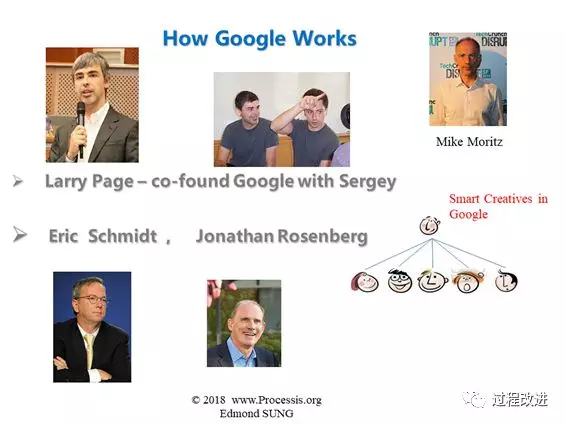
\includegraphics[width=10cm]{香港敏捷2.jpg}

接下来,我会借用谷歌的实例,说明敏捷的原则。\\
Eric本来是NOVELL的CEO,2002年加入了谷歌当CEO。第一天进办公室的时候,他发现风格跟其他东岸的公司完全不一样,例如他的办公室不大。过了一两天以后,竟然有个工程师走过来说:``我们那边太挤了,我看你那边还是挺宽松,我可否搬到你这边来?''\\
"为什么一个工程师还可以进CEO的办公室占位置?"\\
Eric虽然心里觉得很奇怪,
但新来公司,不熟悉谷歌的文化,他便回答:好的,欢迎,没问题。\\
谷歌是有两位斯坦福的研究生创立的,可能大家都知道它是以搜索引擎起家,虽然小,但是技术很厉害。所以开始被当时的巨无霸微软看成是下一个攻击和收购的目标。微软擅长用各种手段打击竞争对手,以垄断市场方面。

董事会的Mike 就发邮件提醒他要准备应对微软的策略
(微软会对有威胁的新公司极力打击)。\\
Eric进了公司后不久,创始人Larry
Page也聘用了另外一个很资深的管理者Jonathan,所以Jonathan和Eric就担起这个任务,要做一个应对微软的计划书,他们都是职场老手,有很资深的商业经验,他们就用传统的方式做了一个详细的业务计划书,计划在未来两年时间如何部署、准备。
计划书很详细,有很多数字支撑。\\
Jonathan很有经验,觉得这个计划还是挺完备的,就拿给创始人Larry看,Eric也在场。\\
Larry 看了几分钟后就问Jonathan:以前试过你们的团队超越了你的计划吗?\\
Larry看Jonathan和Eric好像不太理解,继续说:你见过哪个团队的表现能超越既定目标?你的团队研发过比计划中更出色的产品吗?\\
Jonathan 和 Eric都无法回答。\\
Larry说:如果是这样,计划还有什么意义?\\
最后Larry说一定还有比计划更有效的方式,于是让他们去和工程师谈谈。
他们便发现Google公司的工程师都是既有技术能力,也很有商业头脑的创意精英
(Smart Creative),不需要用硬性的计划来推动。计划反而会妨碍他们的创意。\\
这故事让学员知道要敏捷必须具备一些基本条件:敏捷不是一个万应万灵的魔术棒,不是照着去做便会敏捷成功。\\
另一方面 YAHOO 上市后 便有了各样的 ``大公司''病 ------
官僚化的管理,导致最终被收购。

比如在Google的一些内部讨论中,做决定不只是依据提出者的公司地位、权力,
一些由高管提出的意见不足同样可以被工程师推翻
,Google叫这些横行的管理者为河马(HiPPO : Highest-Paid Person's Opinion)
, 下午做活动练习时 不少组员 常常提到自己公司确实有不少河马在横行。

\hypertarget{ux7f8eux56fdux8d39ux57ce-weisbordux6545ux4e8b}{%
\subsection{美国费城
Weisbord故事}\label{ux7f8eux56fdux8d39ux57ce-weisbordux6545ux4e8b}}

X-Y理论能让我们更理解敏捷开发的原则,每当一些敏捷ACP班学员质疑捷开发是否确实能提升团队的生产率,我就会用
以下故事,让他们感受如何让团队自主管理的过程:

60年代, 复印机还未普及,很昂贵,所以为各类公司客户提供印刷服务有市场,
这故事的主人翁是某美国东岸一家印刷公司的老板儿子Weisbord。
他一直都没有接受什么正式的管理培训。 他有一个好朋友 Don
在国际大公司已工作了20年,
Don推荐Weisbord说:``很多大公司已经开始推进团队自主管理,提升生产率,
你可以先读 X-Y理论 (McGregor `Human side of Enterprise')一书``

X理论:\\

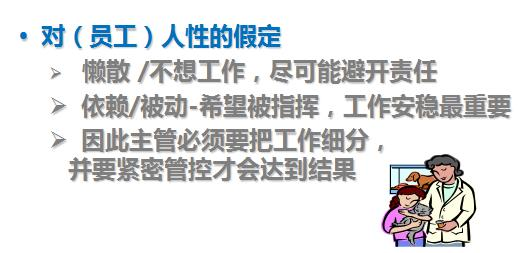
\includegraphics[width=10cm]{0A_Agile_stories_p2.jpg}\\

Y理论:\\

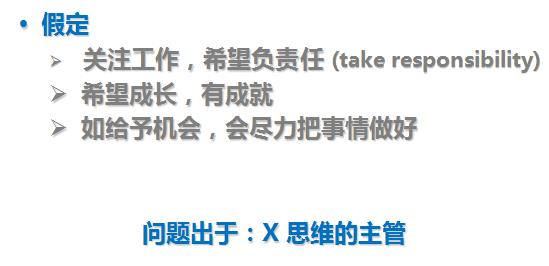
\includegraphics[width=6cm]{0A_Agile_stories_p3.jpg}\\
Weisbord本来只想看看有多厉害,但他结果一口气一周末读完全书。他发现自己公司到处都是都是X理论管理:\\

\begin{itemize}
\tightlist
\item
  工作分得很细,每员工不清楚全局
\item
  任务都是依赖主管分配
\item
  员工遇到问题、困难,交给主管处理
\item
  员工上下班打卡
\end{itemize}

他觉得这方式应该可以帮公司提升,但他担心但靠自己推动不了这个改革,
他便请Don过来正式加入公司。

他们分析公司业务最大问题是订单处理部门(Order Processing),
每个订单处理工作分到五、六个任务,员工只管被分配的任务,例如:

\begin{itemize}
\tightlist
\item
  筛选客户邮寄地址,邮寄印刷样本
\item
  输入订单
\item
  检查客户的信用
\item
  发起内部生产订单
\item
  用打字机打发票邮寄出去
\item
  收到的支票,对上那些应付账
\end{itemize}

公司平均每天要处理200到300个订单,
但因为工作分得很细,如果某个任务(如输入订单)有一、两人缺席,
便严重影响整个流程,效率会降低一半。

针对这问题,Weisbord 计划改革,把这部门的人分成多个4-5人团队,
把公司的两万个客户按地区分到各团队,每个团队有自己的客户名单,打字机等设备,
希望可以增加部门的灵活度和生产率。

Weisbord与5位小主管(supervisor)商量,2位很赞成,2位中立,其他1位觉得不会成功。
Weisbord决策启动这改革,与Don开始重组部门。

\hypertarget{ux5f00ux59cbux56e2ux961fux5236}{%
\subsubsection{开始团队制}\label{ux5f00ux59cbux56e2ux961fux5236}}

开始时问题非常多:

\begin{itemize}
\tightlist
\item
  B物流公司运送出错,送到另一个城市,怎么办?
\item
  D团队误解了生产的步骤,怎么办?
\item
  C团队的样板工人,刚入职3周,对我们公司产品线不熟识,怎么办?
\end{itemize}

原因很简单:本来每个人以前都只懂自己的一小块工作,以前问题都是由小主管处理。现在自主团队没有主管,都要靠团队自己想办法,像瞎子摸象。

但问题确实太多了,没办法,Don建议每周开会讨论。
他们从未有每周开会的习惯,Weisbord本来以为开会浪费时间,把时间用于生产更实际。
问题一直都非常多,延续了一个月

Weisbord开始怀疑这X-Y理论,只是大学象牙塔里的玩意,难以真正用于实际公司环境。
Don也没有更好的建议。

Weisbord开始有撤销整个改革的想法,返回本来的组织架构,
Don还希望Weisbord稍等一两周,看看有没有好转。但Weisbord觉得一直这么多问题,严重影响公司运作,也难以与父亲交代,想在下次开会时向大家宣布变回本来架构。

到了第五周开会:\\
Weisbord,与以前开会一样,先问: 大家有什么问题?\\
沉默,几分钟后,某组长说:没有问题。\\
Weisbord: 为什么会没有?一直这么多问题\\
:(心里想,一定是你们也放弃了,连问题都不愿提了。)\\
另一组长回答:我们今周没有什么问题,遇到的问题都在以前的会议里面被解决了。\\

\hypertarget{ux6548ux679c}{%
\subsubsection{效果}\label{ux6548ux679c}}

改革的后果中本来低于每天一天300个订单提升到400。
员工出勤率也改善,缺席率也降低到接近零。

改革后的订单处理部平面图: 

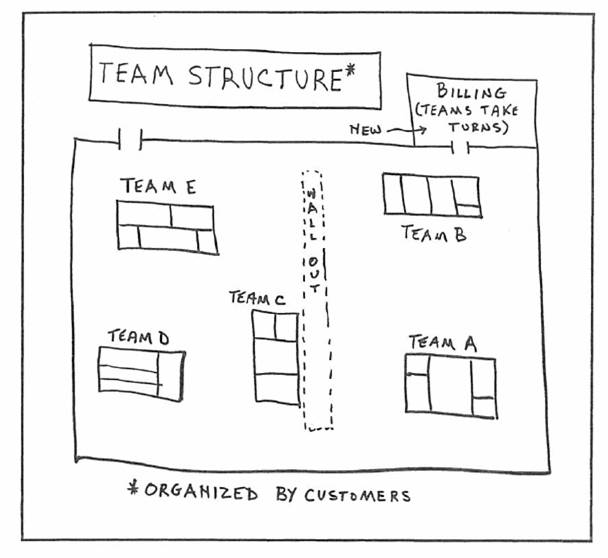
\includegraphics[width=10cm]{0A_Agile_stories_p5.jpg}

(团队自主改革前,小主管们为了减少各功能之间在处理订单引起的争吵,特意在中间加了一道墙;后面团队们一致建议把墙拆掉。)

Weisbord事后回顾:所有改变,重组都需要时间磨合,过程中管理者的支持非常重要,如果管理者不能坚持,面对并解决面对的困难,便会以失败告终。

\hypertarget{google-ux4e0e-weisbord-ux6545ux4e8bux7684ux542fux53d1}{%
\subsection{Google 与 Weisbord
故事的启发}\label{google-ux4e0e-weisbord-ux6545ux4e8bux7684ux542fux53d1}}

如果员工具备知能,管理者便应尽力给员工平台,让团队自主发挥员工与公司都受益;
管理者不仅仅定目标,计划,发号司令,更应该是一位导师,辅助团队成长。

\hypertarget{ux5bf9ux654fux6377ux5f00ux53d1ux56e2ux961fux7684ux542fux53d1}{%
\subsection{对敏捷开发团队的启发}\label{ux5bf9ux654fux6377ux5f00ux53d1ux56e2ux961fux7684ux542fux53d1}}

将前面的故事/研究与敏捷ACP的原则和思想进行对比,也发现很多相通之处。

比如在ACP D1:
原则和思想的第九点,强调一个领袖是服务于团队的,而不是发号施令者,才可以让下面的人更好地发挥。

第五点,领袖要创造一个团队环境,让每个人可以放心做实验、犯错。

都与5级经理人的特性相似。

(详见下面 ACP 后面5点的中文翻译 )

\hypertarget{ux654fux6377ux7684ux539fux5219ux548cux601dux60f3-agile-principles-and-mindset}{%
\subsection{敏捷的原则和思想 Agile Principles and
Mindset}\label{ux654fux6377ux7684ux539fux5219ux548cux601dux60f3-agile-principles-and-mindset}}

大家理解敏捷背后的思路后,下一部分会介绍一些量化敏捷开发的方法与案例,最终
会说明如何满足下面的ACP 原则:

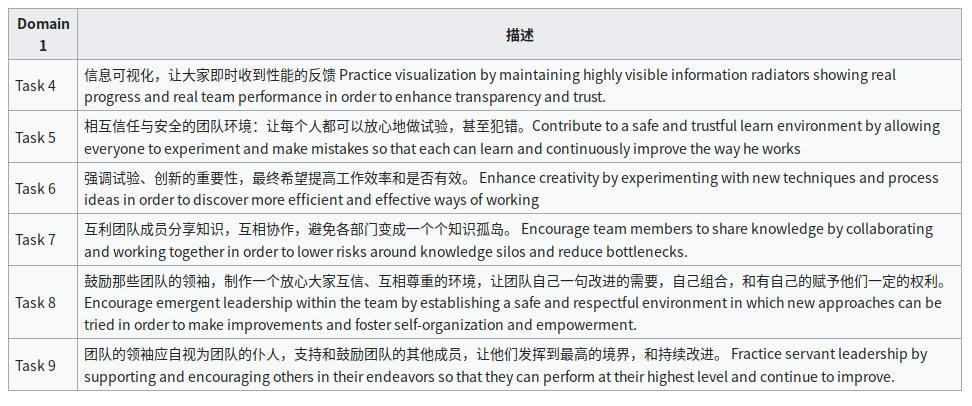
\includegraphics[width=10cm]{Screenshotfrom2022-01-23-1.jpg}

  %
\part{度量与分析}最后部分的重点是量化敏捷开发,很多管理者都知道量化很重要,但往往因未把握度量与分析的思路,效果适得其反。这部分会先分享量化管理的常见问题,然后介绍一些案例,最后以形式帮助有兴趣的团队可以尽快在冲刺回顾复盘中尝试。\\
\chapter{利用数据提升} % Introduction chapter suppressed from the table of contents

Q:我每次都跑全量,引入低码平台,更多的是在需求设计阶段做好质量保证,
所以我们很注重量化质量管理,能否通过自动化来统计分析?
如何通过量化或工具方式实现自动评审?

A:为什么你觉得自动化会帮到你们?

Q:最近我们搞度量, 发现员工就会造数据, 结果导致失真,
度量哪里就造哪里, 所以还是想通过工具代替人工方式

A:现在我明白为什么你想自动化

Q:现在我们的主管很反感度量,一度量就有人造数据

A:度量本来是好的

Q:是的,就是大家知道算法原理就开始造假。
因为我们搞了红黑榜,很多人会想办法。

但很多人头脑都很聪明,但用于不合适的地方。

您的故事 验证了我度量与分析培训课都会分享的故事:

\framebox{%
\begin{minipage}[t]{0.97\columnwidth}\raggedright
利用数据提升管理

\begin{itemize}
\tightlist
\item
  某软件开发公司鼓励员工利用数据做过程改进,开始时很多成员不太接受但管理层一直支持坚持做下去
\item
  过了七个月,大家确实看到这种利用数据的过程改进使得团队质量跟生产率提升明显。
\item
  管理层觉得这个量化很成功,便把一些系数作为考核项,
\end{itemize}\strut
\end{minipage}}

猜猜会有什么后果。。。\\
后面团队的生产率就没有任何再提升了,
半年后,大家都觉得度量数据没有作用,管理层也不再用这些度量指标来考核了。

\textbf{度量主要是帮我们做分析找出根因做改进而不是仅仅为了监控}

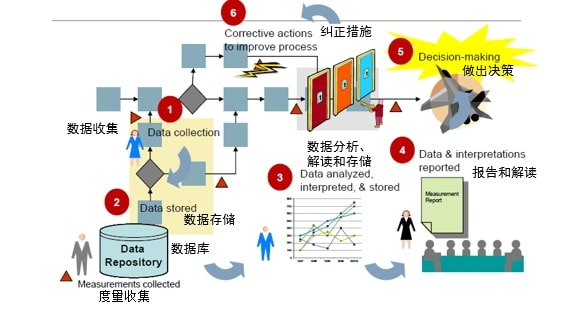
\includegraphics[width=10cm]{Ma4CarScreenshot_2021-12-27_205004.jpg}

\framebox{%
\begin{minipage}[t]{0.97\columnwidth}\raggedright
几十年前,我在企业做管理时,某一次花了三个月时间梳理一下工程的流程,大家都非常忙,都必须要自己加班加点腾出时间来做。\\
完成后,我便与大老板说``我们辛辛苦苦做了这些成绩可否公司给一些奖励?''\\
他便问我``我没看到你这次工程的流程梳理为公司增加了收入,公司没有额外收入,哪里有钱给你们奖励。''\\
我当时有点生气,但回想一下,他确实有道理。\strut
\end{minipage}}

Q:我们有很多数据统计分析,比如看测试用例与需求的比例。
其实客户发现的缺陷比例也降低了,但因为我们这行对质量特别注重,产品经过多年的逐步演化,过程很复杂,导致软件缺陷的修复很耗时,客户不太满意。\\
而且公司要求交付的频率要比以前高了很多,我们团队做这些分析都忙不过来,所以需要员工设自动化工具等加快速度才可以。

让我给你看看我们大数据分析。。。

A:我看好像你们是对所有项目的统计分析?

Q:是

A:你们管理者花精力分析数据出发点是好,但问题是团队会依赖你们管理者做分析
并非团队自己动脑筋持续改进。

Q:是的很多开发人员都觉得质量是你们(管理层)来管

A:你说的很好,这正是妨碍提升质量的最大障碍。
每个开发人员(甚至需求人员/产品经理)都要意识到质量好坏把握在自己手上,不能靠你们管理层或后面测试。
每次回顾要让他们把这些排除源头识别出来,他们才会感觉到自己的水平多差,前期遗漏了多少缺陷。

三十年前,Infosys
公司也是经历过这种过程,先让开发从数据发现很多缺陷都后期才被发现,导致大量返工。开发才有动力改进,把缺陷的发现提前,最终软件开发质量。
所以更快的自动化工具帮不了你们。

昨天与成都客户讲,要开始量化管理,不是自动化工具,而是个人,好比准备9个月后跑半马,必须锻炼和统计。

Q:你说的我都没想过,但觉得还是挺有道理的。

A:这点也是我昨天跟成都客户强调的:\\
\textbf{让所有员工改进整个系统问题}

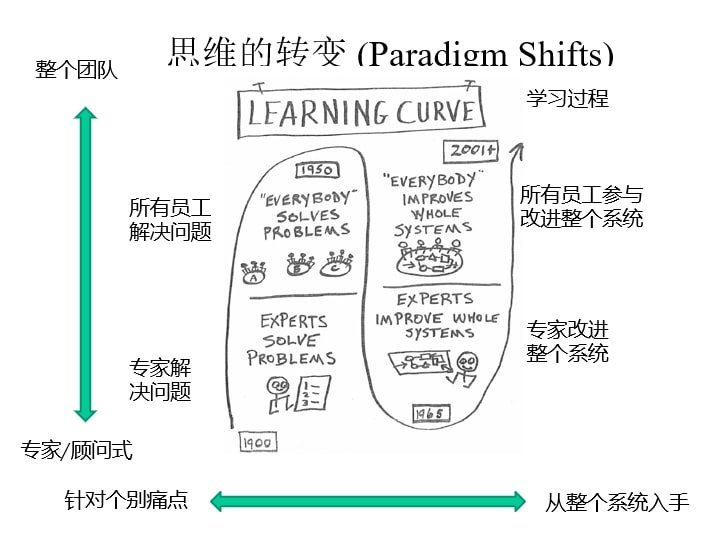
\includegraphics[width=10cm]{ImproveWholeSystemScreenshot_2021-12-27_204408.jpg}

总体的分析还有另一不足:各个项目特性不一样,你们现在几十个项目总体趋势分析,
很可能找不对根因,因每个项目的问题(根本原因)很可能不同。
比如,同样是一个测试用例比例数,你的范围就很宽 -
从最低的0.3到最高的超过200!但你们取平均值5.1 来做分析。

收集数据也是问题,因收集数据是挺花精力的工作

Q:完全100\%同意

答:但正因为不同项目有各种特性,要对收集到的数据做分析也很耗时。
这些辛辛苦苦做出来的分析报告其实不仅仅是给高层(或者项目经理),
在每一个团队成员都看到才有意义
。(度量分析要反馈回数据提供者,他们才有动力继续收集数据)要把那些分析好的报告再跟每一个团队成员解释上要花多大精力?

如果把数据分析下放到团队自己搞,便灵活很多了;也正因为他们有参与收集和分析讨论,
你们也可以节省很多沟通的成本。

所以你们领导应该定位自己是内部老师,辅导团队怎么做好数据分析,效果会更好。

Q:就当团队自己讨论便可以得到改进吗?不需要我们领导?\\
答:只要他们有一个较高的目标,不要低估人的潜力,只要他感觉到现状跟目标有差距,他也想挑战自己,达到这个高的目标。最近看一个电视节目播放三个滑翔伞者挑战海拔6250米幺妹峰的过程,他们都很有经验,装备齐全,比如贴在鼻子供氧的设备等等。他们一直观察天气情况,因为滑翔伞必须要借用上升的气流才可以上升。其中一位一直观察小鸟飞行,就选择鸟的方向去飞,确实有一股上升气流,中间经过如大雾,差点撞上山等惊险过程,最终完成,他开心极了(详见附件)。\\

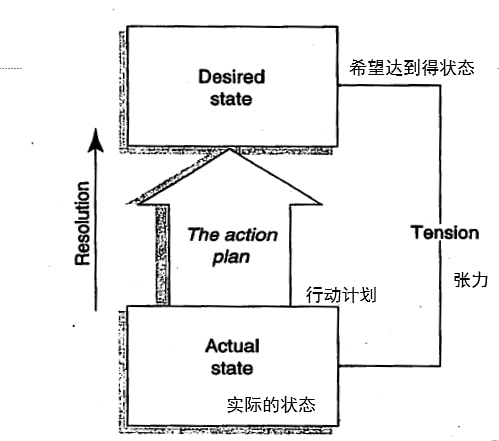
\includegraphics[width=10cm]{Tension2ImproveScreenshot_2021-12-27_204553.jpg}

希望达到的状态,就可以克服种种困难,团队也一样,如果有很高的目标,都会想办法,尽力完成,人的智慧无限,领导要相信团队的潜力。所以我们说度量就是让他们可以实际看到目标与现状的差距。具体怎么做?他们最清楚。刚才滑翔伞的案例,是否可以有一个经验丰富的远程教练教他们怎么做?不可能,都是要靠现场的经验,依据实际的情况去寻找合适的机会,有可能成功,有可能失败。\\
希望团队提升,达到那个最高目标也一样,不可能有一套所有团队适用的方法。我们作为领导主要是作为一个教练支撑他怎么去做,最终还是要靠自己。团队的成长跟一个小孩的一样。比如你看见现在年轻的父母,也可能是当一个小孩。不让他自己走路而坐学步车,不让他自己吃饭而喂他,你估计他后面可以独立成长吗?这样会造成过度依赖,对成长不好。\\
Q:你说都是个人提升例子,整个公司提升就没你说这么简单。\\

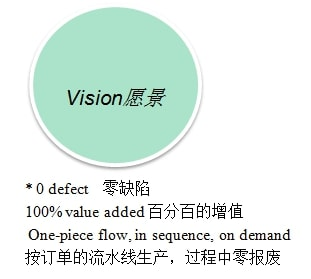
\includegraphics[width=10cm]{远景1.jpg}

A:是的,但道理还是一样,比如你看看上面这个图。假设你是50年代的一家汽车公司,你的销量、成本、效率就那些先进的世界级汽车公司差很远。你觉得能达到图中这个零缺陷、零废物、一次性流水线生产目标吗?\\
问:不太可能,所有过程都有极限,到了一定程度就无法再提升了。\\
答:现代的汽车生产过程差不多可以达到上以上的水平,刚才我说的就是现在世界最大的汽车公司丰田。当时他觉得美国汽车公司那种依据福特的生产线做法,不能适应不同客户的定制需求,而且从原材料到生产出汽车很慢,他就一直研究如何达
Just In Time
目标。现代,5、60年后,这种生产方式已成为世界级的标准生产流程,如英国牛津日产为德国宝马公司生产魅影汽车的生产线,可以做到每个步骤都没有多余的库存;
而且从原材料(钢材)到完成生产出汽车只需要24小时。\\
Q:如何激发团队战斗力,是否有一些建议和方法?\\
听你的故事,每次迭代量化目标要由团队自主分析,设定,怎样做?

A:问得好,很多想利用敏捷开发做提升的公司也问。
我在下一篇"量化质量管理FAQ"里有解答您这问题。\\
大家可能也遇到类似的困惑,后面会先分享一些案例,然后用问答形式解读这些方法如何能解决以上问题。本章用以下故事总结:

\framebox{%
\begin{minipage}[t]{0.97\columnwidth}\raggedright
\begin{itemize}
\tightlist
\item
  新上任的总监很了解前期评审的重要性,他发现团队一直都没有评审的习惯,并下令所有项目必须要做评审,而且要把评审的数字定期上报。总监为了鼓励团队做评审,也对评审效果做了一些奖励措施。所以每次在月会上,总监都会听到团队关于评审的记录、报告。\\
\item
  但其实他不知道的是,团队实际上没有做任何评审,可能只是在酒吧聊天的时候,随便写一些出来变成报告上交。后面总监终于发现真相,非常生气。\\
\end{itemize}\strut
\end{minipage}}

\textbf{经验教训}:

\begin{itemize}
\tightlist
\item
  单靠上层制定方法,下面不明白为什么要做这件事,只是听指挥去执行,往往得不到什么改进效果。改进必须是源自团队本身才可以持久。更应参照XY理论,让团队自发解决问题,并提升。
\item
  只优化了某一个过程,不一定能改进整个系统,必须``所有人参与改进整个系统''。在复盘时,让团队回顾冲刺数据,并一起讨论如何在下轮冲刺改善。
\end{itemize}

\hypertarget{ux9644ux4ef6ux9996ux4f4dux901aux8fc7ux65e0ux52a8ux529bux6ed1ux7fd4ux4f1eux98deux8d8aux5e7aux59b9ux5cf0ux6d77ux62d46250ux7c73ux7684ux4eba}{%
\subsection{附件:首位通过无动力滑翔伞飞越幺妹峰(海拔6250米)的人}\label{ux9644ux4ef6ux9996ux4f4dux901aux8fc7ux65e0ux52a8ux529bux6ed1ux7fd4ux4f1eux98deux8d8aux5e7aux59b9ux5cf0ux6d77ux62d46250ux7c73ux7684ux4eba}}


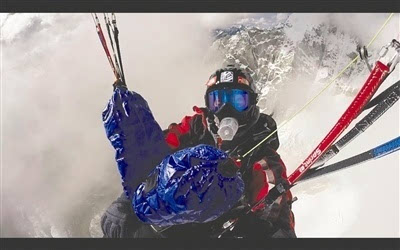
\includegraphics[width=10cm]{滑翔2.jpg}

飞行中的李群国\\

\begin{itemize}
\tightlist
\item
  2016年,34岁的李群国以6356米的高度环绕幺妹峰峰顶一圈\\
\end{itemize}

10月18日,一支三人飞行团队在四川阿坝州四姑娘山完成了一次极具挑战的探险:他们用无动力滑翔伞的方式飞越了海拔6250米素有``蜀山皇后''之称的幺妹峰。其中,34岁的李群国经过2小时40分的飞行,以6356米的高度在环绕峰顶一圈后,顺利返航。\\
\textbf{挑战}\\
云终于散开了一点!10月18日中午12时,在位于四姑娘山南侧海拔3950米的朝山坪,李群国和他的队友------中国滑翔伞国家队教练元林朝、中国越野飞行记录保持者宋俊明三人齐齐地望向远处。``应该差不多了。''元林朝转过身,招呼着现场的人员做好飞行前的最后准备。\\
他们的目标正是眼前的这座雪山------素有``蜀山皇后''之称的四姑娘山幺妹峰。在这之前,他们已经等候了近三个小时。\\
最先起飞的是宋俊明。要想让滑翔伞持续升空,必须依靠上升气流的辅助,但宋俊明经数次寻找,最终还是没能找到上升气流,只得放弃飞行,安全降落。而此时,天气再次被云雾笼罩。元林朝和李群国只好继续等待时机,期望天气好转。\\
一个小时后,转机再次出现,元林朝和李群国决定再冒险一试,于是,两人先后起飞。``恰好就碰到了好运气。''李群国介绍,飞出不久,就遇上了一股上升气流,高度慢慢爬升到了4800米。接着两人尝试着靠近第一座大妹峰,靠近后又遇到了下一股上升气流,便继续往二三妹峰靠近,看起来一切都很顺利。\\
~\\
不过,在靠近幺妹峰时,峰顶再次出现了云雾。``云雾里飞行好比大雾里开车一样,是极其危险的。''尽管已经飞至6100米高度,元林朝经过判定,还是选择了返航。但此时的李群国却冒了一把险,凭着气流继续上升,并成功越过了幺妹峰,``当时就是想突破一下,虽然确实有些冒险,但我们成功了,这个团队成功了。''\\
\textbf{惊险}\\
上升途中突遭下沉气流,瞬间下跌100米\\
其实,李群国的成功飞越同样伴随着惊险。用他自己的话说,``像是一场玩命,但决定了要去挑战,就已经有了心理准备,探险都有可能付出代价,哪怕是生命。''\\
就在李群国过了三妹峰时,他遭到了一股下沉气流,高度重新下降到了4800米左右,``这个时候有可能就找不到机会再攀升了。''于是,他调整了飞行方式,绕到了幺妹峰的西北角,准备降落。而就在降落的过程中,又再次遇到了一股很强的上升气流,他内心一阵暗喜,高度又迅速地上升到了5500米左右。\\
然而,这股强大的上升气流却也伴随着致命的危险。``往往在强上升气流的边缘就会伴随着强下沉气流,一旦遇上了就会非常快速地往下掉,尤其是在高原地区,气流的复杂程度更大。''李群国说,而自己却正好遇上了这股伴随的强下沉气流。\\
突然间,李群国就失去了动力,伞翼出现变形,整个人和滑翔伞开始不正常地下降,伴随着旋转和俯冲,做着自由落体运动。``一瞬间的工夫,就掉下了100多米。''好在对于已经从事滑翔伞飞行达15年的他来讲,这样的情况仍在他的控制范围内。经过一系列的调整,才最终恢复正常飞行。\\
李群国最后的飞行高度达到了6356米,超出顶峰达100多米,而此时眼前的云雾也为他打开了一扇窗,云缝里的幺妹峰让他激动不已,``太震撼,已无法用言语表达。''\\




\chapter{量化敏捷开发案例} % Introduction chapter suppressed from the table of contents

今天培训的对象是老客户,但与3年前不同,这次从公司前台处走到总监办公室足足花了2分钟。
沿途要经过他们的三个开发大厅:每个大厅坐着70到80人。规模与3年前相比,大了很多,新员工绝大部分是做项目开发测试等技术工作。总员工数量从不到200人到超过600,且还在陆续增加,所以虽然两年前才搬到这个3000平米的新办公室,现在也基本上坐满了。

我说:公司发展很快,跟三年前完全不一样了。\\
总监:是的,CEO特别支持公司的发展,在这方面做了很多投资。以前我还能喊出每个员工的名字,现在新人太多,很多都脸生。例如,只见这几百人每天在电脑前工作,但每个人的质量与生产率等差异却看不出来。为了管理好这么多人员,不得不依靠系统。

\hypertarget{ux516cux53f8ux80ccux666f}{%
\subsection{公司背景}\label{ux516cux53f8ux80ccux666f}}

多年来,这家公司一直做医疗IT解决方案,门槛很高,不仅要懂IT,也要懂行业知识。医院,或医疗机构,都对质量有要求。\\
工作压力也很大 ------
去年业务扩展很快,除了要增加软件产品数量以外,也非常注意客户满意度。总监觉得客户满意度主要由两个因素组成:

\begin{enumerate}
\tightlist
\item
  客户要的功能能否及时反应
\item
  能否提供他们确实要的东西
\end{enumerate}

针对第二点,公司用系统记录了所有客户的问题,统计这些客户反馈的缺陷。要求过程改进小组,按月统计客户反馈的缺陷,看是如何逐步到得到改进、不断完善。公司也关心总研发成本。

\hypertarget{ux4ee5ux964dux4f4eux8d28ux91cfux6210ux672cux4e3aux76eeux6807}{%
\subsection{以降低质量成本为目标}\label{ux4ee5ux964dux4f4eux8d28ux91cfux6210ux672cux4e3aux76eeux6807}}

问:你们的业务改进目标是什么?\\
答:研发成本要降低。\\
问:具体是降到多少呢?\\
答:高层没说,只是说目标要降低100万。\\
我问:为什么定100万这个数?\\
总监答:其实我心里也没有底,但大老板很坚定要控制研发成本。必须要做,没有办法。但你不是说过容易达到的目标不是好目标,所以我们就定``减少一百万''要求过程改进小组自己想办法。
如果最终没有想到更好方法,唯有减少测试工作,降低成本。

问:从需求到最后验收, 您觉得那个过程的缺陷返工量最大?\\
答:应该是越后越大\\
问:是的,而且返工工作量不仅仅按比例增加,是按倍数增加

例如,依据一些美国IT公司的统计:\\

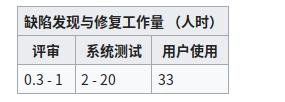
\includegraphics[width=10cm]{Screenshotfrom2022-01-1801.jpg}

但很多研发团队只依赖测试来保证质量,导致大部分缺陷都要等到系统测试甚至客户验收时才被发现。

\framebox{%
\begin{minipage}[t]{0.97\columnwidth}\raggedright
如何通过提高评审效率来降低质量成本 (Economics of Software Quality)
质量成本由三部分组成:

\begin{enumerate}
\tightlist
\item
  失效(Failure)成本\\
  把缺陷修复好的成本,包括在客户现场被发现的缺陷。
\item
  评测(Appraisal)成本\\
  包括各类测试,如系统测试,集成测试,单元测试等,所花的工时
\item
  预防(Prevention)成本\\
  包括技术评审 (注:有些人把评审归为评测成本,这里按 Mr.Juran
  定义,归属于预防成本)
\end{enumerate}

加大预防(评审)的力度,可大大减少失效成本(如测试和验收工作量)

例如,开发10万行代码(包含新增和变更):\\
场景1:评审效率只有50\%:\\
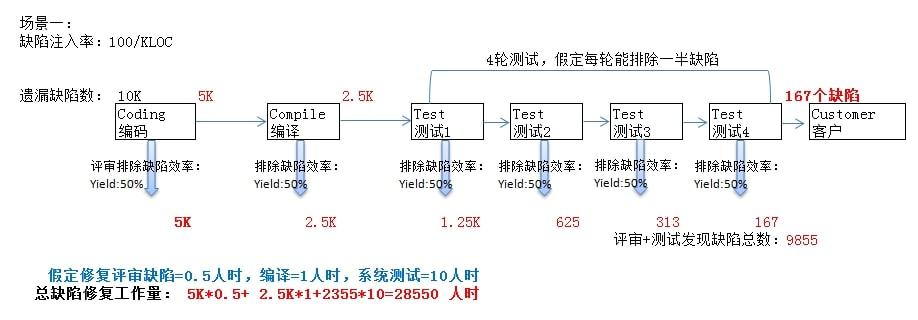
\includegraphics[width=8cm]{缺陷场景1_2_0.jpg}\\
场景2:评审效率达到75\%:\\
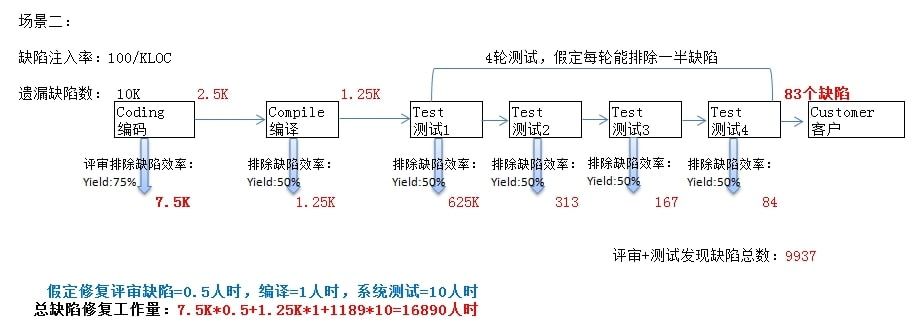
\includegraphics[width=8cm]{缺陷场景2_2_0.jpg}\\
\strut
\end{minipage}}

从以上例子看到,提高评审效率不仅能把交付给客户的缺陷减半 ,
更重要的是能够降低质量成本的失效成本,为了提高评审效率,工作量可能会略有增加,评测成本基本不变
。 把代码评审效率从50\% 提升到75\% 便能节省 1,462 人天 {[}=(
28.5-16.9)/8{]} (假定1人天=8小时),节省超过40\%。注意:场景1与2
过程中评审或测试排除数基本不变,同样大概 9.9K,只是场景2
把2.5K测试缺陷推前在评审发现,但因修复系统测试缺陷要10人时,但修复评审缺陷只需0.5人时。不同公司的缺陷修复工作量可能不同,但只要后面系统测试缺陷修复的工作量比评审的工作量大,那么把缺陷从后面的测试前移到评审发现,便能大大减少返工的工作量。

评审通常包括需求、设计、代码
评审,另外可以增加架构评审,原型评审。例如,如需求评审有客户参与,效率/效果都会更好。

总监开心地说:对了,我们开发好像一直都没有太注意评审,
觉得浪费时间,也没有评审出多少缺陷。
听你的例子,只是把评审效率从50\%提高到75\%便可以降低四成成本,如我们能从0\%升到50\%应该也能节省不少,我觉得降低一百万这目标应该有希望了。
我马上要求质量部发布评审规范与过程,并要求每一个团队都必须按这个去做。\\
问:这个例子中的质量成本(主要是失效成本)降低了四成,虽然未包括开发本身成本,但确实也省了不少。但请注意改变人的习惯很艰难,不能单靠发布流程。
必须先从个人习惯入手。你估计导致质量成本增加的主要原因是什么?

总监答:很多原因,例如前面需求没做好导致设计编码有误。

我说:去年一家我们辅导的公司,每次做完迭代冲刺后,都会叫上所有组员,包括产品经理、测试开发一起看看本次迭代的问题,讨论一下那几十个缺陷是源自哪方面?是否因为需求没做好?还是开发编码本身的问题?针对当次回顾复盘反馈最多的问题,并讨论它的根因后,在下一个迭代中采取一些针对性的改进措施,希望下一个迭代能减少对应的系统测试问题。\\
例如,有一次回顾时候就发现有一个功能升级模板,因为产品经理没有把握好客户的实际要求,导致我们那次迭代做出来这个功能不满足客户要求。虽然有做需求评审,但大家未能发现这需求问题。过程改进组就更新了需求评审检查单,增加一项,希望以后会减少同样的问题。另外,我们发现除了需求以外,还有很多是因为代码本身写得不规范,比如,有很多分支,常数也没有处理好。这些都在后面的系统测试和一些客户发现的问题反映出来。改进组便相应地加强了代码评审和代码规范的检查项和样例,来避免再发生同类问题。\\
总监问:有什么效果?\\
我答:其实大部分的缺陷都是人的缺陷防范意识弱,经过几轮培训与辅导,大家便更注意,主管也开始注重,后面的迭代,这类的问题就减少,不再是主要问题。\\
你们现在不是要求项目组在每个冲刺(迭代)后都必须要做个小组内部回顾吗?可否安排我参加,观察一下。\\
总监:正好我们下午应该有一个项目组要做内部回顾复盘(Retrospective),欢迎您来看看。

\hypertarget{ux4eceux9879ux76eeux51b2ux523aux7684ux56deux987eux590dux76d8ux5f00ux59cb}{%
\subsection{从项目冲刺的回顾复盘开始}\label{ux4eceux9879ux76eeux51b2ux523aux7684ux56deux987eux590dux76d8ux5f00ux59cb}}

在回顾复盘现场,测试人员投影了本次迭代的缺陷分析,展示下面两个缺陷分布图
:

\begin{itemize}
\tightlist
\item
  开发人员排名(最多的排头)
\item
  按模块来区分(最多的排头)
\end{itemize}

团队组长便按照缺陷的严重程度询问每位开发人员 -\/- 是否知道怎么修改?\\
大家都说知道了。组长要求大家提出问题,如果没有问题就准备散会。

我问:大家好,你们有没有兴趣做个``整个团队一起改善整个系统''实验。
后面让我们暂时抛开自己本身是什么岗位。
大家一起看看有哪些地方能减少缺陷?

例如,除了按照人员与模块区分。 我们可否把缺陷简单按下面类型分组 :
需求/设计/编码 ?

他们就让测试人员,展示本冲刺发现的34个缺陷,让大家逐一讨论,找出缺陷是源自哪过程
,最后把总数写在在白板上:


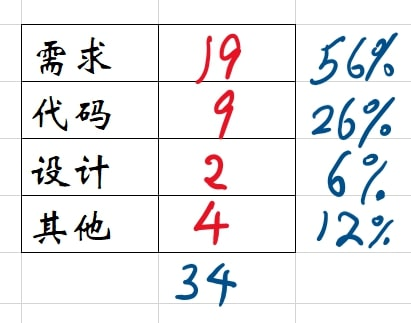
\includegraphics[width=10cm]{DefectsBySourceScreenshot_2021-09-20_155232.jpg}

让我们看看是怎么分布? 为什么这类缺陷最多呢?大家估计背后是什么原因?
针对需求(最多的类别),我辅导团队利用KJ方法{[}详见附件A2{]},识别主因。最终汇总成以下结果:\\

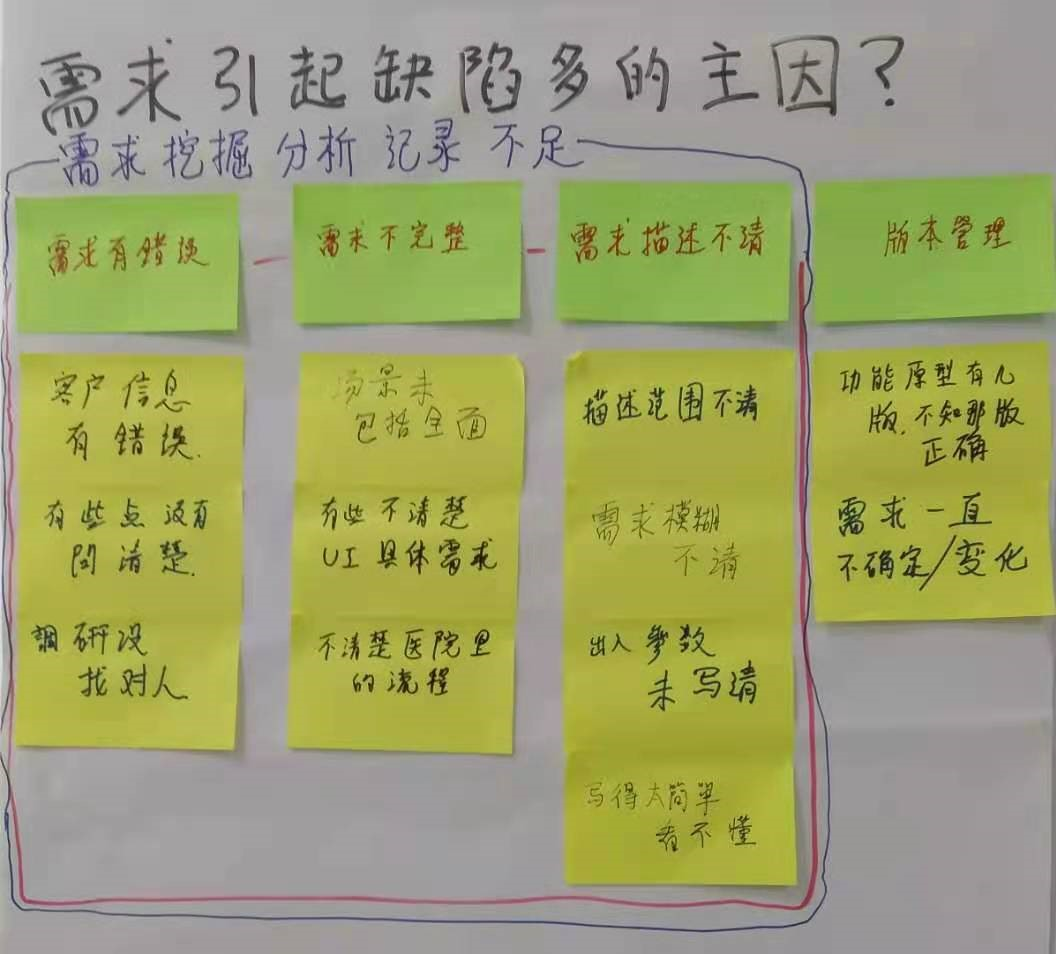
\includegraphics[width=10cm]{微信图片_20210920125228.jpg}

\hypertarget{ux4eceux95eeux9898ux5206ux6790ux5230ux6839ux672cux539fux56e0ux5230ux884cux52a8}{%
\subsubsection{从问题分析到根本原因到行动}\label{ux4eceux95eeux9898ux5206ux6790ux5230ux6839ux672cux539fux56e0ux5230ux884cux52a8}}

我问:针对我们刚才一起找出的主因,根本原因是什么?
如何可以避免同类缺陷再发生?

答:要加强对需求人员的培训,提高他们的能力。\\
总监说:我年初已察觉到确实很多需求没有表达清楚。
导致开发出来的东西不符合客户要求,或不是客户要的。

我见过以下用户故事:

\texttt{病人或他的家属能容易找到他选择的服务。}\\
\texttt{~理由:他们熟悉网上购物,习惯了方便和快速的响应时间时间。}~\\

我问需求人员怎样才算容易找到,验收标准?

我估计她记得我说过需求必须可测量,她想了一会,说:验收标准:``普通病人能够在6秒钟内通过不超过三个动作定位任意一项服务。''

我说如果把`普通病人'改为`90\%以上的病人'更好。

必须把模糊,有二义性的需求变成可以测量。

所以不能仅仅说 `新功能很酷,很创新',
而应明确验收标准为:引入了新功能的三个月之内,60\%的用户应该用它来完成规定的工作。75\%以上的用户对产品表示赞许。

所以三个月前,我已经开始 准备正式规划产品经理与需求分析师岗位:
要经过挑选,考试,然后培训,达标才能正式上岗。
本来计划两周后会正式公告,现在既然你们问到,我就预告一下。

我说:既然高层已经有长远的规划,我们团队就应该针对下一个
冲刺,我们可以做到的事情。

项目经理说:我们每个岗位都已经尽了全力,没有什么可以做了。\\
我问:你们有做评审吗?如需求,设计评审\\
答:有。\\
问:需求评审发现多少缺陷,设计评审发现多少?\\
答:好像两三个。\\
问:发现什么问题?\\
答:记不清了,当时直接就修改了。\\
问:请问评审总共花了多少时间?多少人参加?\\
答:我们六个人,那次评审大概用了接近2小时。\\
问:2小时?\\
答:我们不仅仅发现需求问题,也一起讨论如何修改\\
问:如果评审只找缺陷,记录,应不会超过一小时,如果大家事前做好准备,估计可能半小时可以完成。所以通常检查(Inspection
)不会当场讨论如何修改。\\
我接着说:我们刚才分析系统测试缺陷,不是识别出超过一半是源自需求吗?为什么我们不能在评审时预先发现?
你们觉得可以下一个冲刺,评审时可以发现更多缺陷吗?\\

\texttt{我立马用5分钟与大家分享有效评审能降提高产品质量,降低成本的例子。}

答:估计应该可以,但不知道怎么做?\\
问:你们评审有检查清单吗?\\
答:没有。\\
问:清单可以帮助我们吸收以往的经验,避免以后同类问题再发生。
例如刚才我们都识别了跟需求挖掘/分析/记录不足相关的具体问题吗?
可否利用这些,更新评审检查单的检查项项,提醒我们要避免同类问题。
如果大家同意,我们现在就行动。我们要改进
便要制定目标,例如计划下次需求评审,系统测试等各过程发现的缺陷数。
这些目标你们可以下周一策划两周冲刺时定。

\texttt{组长安排了小李更新检查单。准备在下次评审前与需求文档,预先发给参评人员。}

我说:谢谢大家,我没有其他要说了,下次回顾,我或总监会来参加,看看冲刺的效果。

\framebox{%
\begin{minipage}[t]{0.97\columnwidth}\raggedright
冲刺回顾与根因分析 回顾时对本冲刺的数据做根本原因分析
是持续改进的最佳实践。\\
我在这案例是按下图的五步来辅导团队,确保
每一位成员都全心投入参与,并从分析形成行动,达到改进效果:\\
\#设置舞台

\begin{enumerate}
\tightlist
\item
  收集数据
\item
  分析,找出根因
\item
  决定做什么
\item
  结束
\end{enumerate}

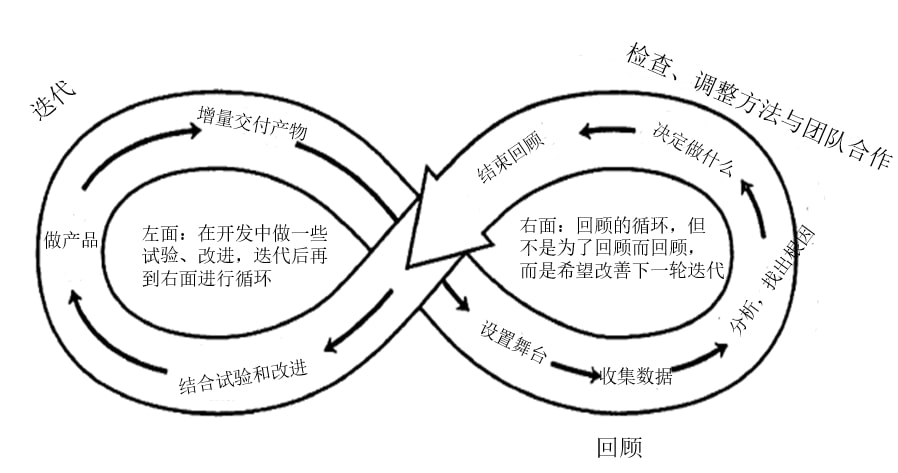
\includegraphics[width=10cm]{RetrospectiveScreenshot_2021-09-21_173119.jpg}\strut
\end{minipage}}

\hypertarget{ux6539ux8fdbux8981ux4eceux4e2aux4ebaux6570ux636eux7edfux8ba1ux5165ux624b}{%
\subsubsection{改进要从个人数据统计入手}\label{ux6539ux8fdbux8981ux4eceux4e2aux4ebaux6570ux636eux7edfux8ba1ux5165ux624b}}

复盘会后,我找了团队的两位开发,她们都是在开发岗位工作了4、5年的女编程员,一位叫小萍(XP)
, 另一位叫`Shirley'(S)

我问:大家觉得刚才回顾会后面的讨论怎么样?\\
XP过了一会说:以前回顾会都是问责,我们做开发的都不敢发言,说多错多。
因为是我负责的模块缺陷偏多,我肯定不愿意在大家面前丢脸。 到后面用
写便利贴方法
(她是指KJ法),我就不怕直说了,其实以往的回顾会都是主持人(项目经理)
讲,我们只是听。

我问:你们觉得刚才在回顾里提到可利用加强评审来减少后面缺陷的返工怎样?\\
XP:
有道理,但现在测试工具都很先进,立马就可以把缺陷暴露出来,为什么还需要
依靠人工查看代码,这样做不是更耗费时间吗?\\
问:好的,首先让我先理解你们现在的开发过程?\\
答:写代码编辑,先自己编译通过,然后自己手工测试一下。\\
(她们的表情好像在说:还听其他组员说您是软件工程20年经验的专家,还会问我这些低级问题?)\\
问:测试之前有没有做设计或代码的评审。\\
答:没有,因为时间都很紧,手工评审很耗时。\\
问:理解。但软件工程界统计过如果同样的缺陷等到系统测试才被发现,可能要好几天才能解决,但如果能在代码评审(或需求评审)中被发现,很可能不到30分钟便能解决。\\
一般情况下,你们需要花多少时间修复在系统测试阶段发现的缺陷?\\
答:没有正式统计过,差不多半天到好几天都有。\\
问:如果像Apache,Eclipse
那类超大型软件,很可能不止。如果要找出答案,便需要数据。
例如,我们现在关心:缺陷数,评审工作量,缺陷修复工作量。
必须要求每人在开发时,自己把数据记录下来,
以数据说话,到后面才知道有没有提升,返工工作量有没有减小。
虽然通过评审尽可能早地发现缺陷是最好的,
但不能只依赖评审,必须也有单元测试。 与评审一样,
单元测试也能帮助我们提前找出缺陷。

S:现在我们都已经用敏捷开发了, 同行评审好像都是上一代瀑布开发年代的事情,
是否已经过时?\\
我说:虽然敏捷好像不强调评审,但极限编程 (eXtreme Programming)
里有结对编程 (Pair Programming) ,
其实也是一种评审。只不过不是等到写完代码后才评审,
编码的同时有人在评审, 所以敏捷并非没有评审,
目的都是希望尽早发现缺陷,防止遗漏到系统测试阶段。
如果你们能在编码时能减少缺陷, 也同样能达到减少缺陷遗漏的目的.\\
S:是否应该通过测试后才评审代码?便可以针对有问题的代码,节省工作量?\\
我说:这个思路看来好像不错,但最大的问题是这会影响评审组找出缺陷的动力。因评审员都知道这软件已经测试过。\\
S:好吧,再前一步,是否应该在通过编译后才评审代码?\\
A:虽然各有长短。我建议先评审,后编译\\
例如编译通过不表示所有的编码格式问题都被找到。
你们都不会再去关注代码的格式问题了,从而导致那些问题(可能10\%)要到系统测试阶段才暴露出来。\\
我问:你们哪位知道如何制定锻炼计划准备六个月后可以参加半马比赛?\\
(S高高瘦瘦很运动型,我猜可能她知道。)\\
XP:必须制定很详细的每周锻炼流程,度量每次的时间、速度。\\
(后来我才知道XP她刚跑完半马,人不可以貌相)

我问:要提升个人的编码能力(质量,效率)就与准备马拉松一样,天天收集数据才知道新方法是否有帮助,有没有改善。你们有兴趣吗?\\
XP答:OK ,但S和我写不同的模块,收集数据是否只是供自己作前后比较?\\
我说:
很好的问题。两个月前,我们陈老师不是教你们用简化功能点来衡量项目规模吗?
如果像你们每个项目都使用功能点,你们的缺陷密度就有可比性了。

XP:如何收集汇总缺陷,统计数据?\\
我说:先由开发人员自己记录,然后在回顾时,由项目经理和组长统一汇总到公司项目数据库中。
大家也可以利用回顾,看看现在和以往的数据趋势,一起分析讨论。\\
我接着说:你们可以按照以下这个数据模板,记录下通过测试与评审发现的缺陷数量,与返工工作量,然后我们做统计分析。
看看评审能不能帮到你们降低修复缺陷的工作量,最终能提高你的代码生产率。以下是以前两位编码人员的个人统计,可以看到如果能通过代码评审发现缺陷,代码生产率就越高:

\includegraphics[width=6cm]{hump291Fig913Student1_2_0.jpg}\\
\includegraphics[width=6cm]{hump292Fig914student2_2_0.jpg}

Key: 评审效率 Yield = 代码评审找出缺陷数 / 代码引起缺陷总数
(=评审找出缺陷数+后期测试发现的缺陷数)\\
:: 生产率 = 每人每周产出多少有效功能点 (FP)\\
你们后面也可以自己做出类似的图。\\
XP:听起来收集数据要花不少工作量,有软件工具自动收集吗?\\
我问:请问你跑半马前,如何做准备?\\
XP:比赛前六个月开始按定好的计划训练,并记录每次实际时间。\\
问:怎样记录?\\
XP:现代跑步的都有电子数字手表,记录每段的开始与结束时间,很简单。\\
我说:统计个人实际工时也类似,编码时记录开始与结束时间,不需要自动化工具。你也可以看看我以前的经验分享《个人如何写程序并记录》\\
难点不是在收集数据花多少时间,而是改变个人的习惯,您刚开始锻炼时估计也应遇过同类问题?\\
XP:是的,好在我们有个跑步团,我看大家都这样做,我慢慢便习惯了。\\
我接着总结说:当你们收集了多轮数据后,便可以分析并制定提升代码质量的策略:\\
每人都有各自的长短。 有了自己的缺陷统计数据后。 改进必须有针对性:
哪一类的缺陷出现最多最严重? 应选择哪个最弱的过程才容易有效果。

最后,预防胜于治疗,最终不能单靠评审与测试,更需要在编码时,注意避免引入缺陷。
真是没有必赢的金科玉律,但有数据才有动力,才有方向,促进改变以往的习惯。
好比减肥,必须每天测量自己的体重一样。
(我看她们的两位体重都正常,应该可以提这个对女性较敏感的题目。)

\hypertarget{ux5efaux7acbux516cux53f8ux5ea6ux91cfux6807ux6746ux57faux7ebfux4e0eux6a21ux578b}{%
\section{建立公司度量标杆(基线)与模型}\label{ux5efaux7acbux516cux53f8ux5ea6ux91cfux6807ux6746ux57faux7ebfux4e0eux6a21ux578b}}

四个月后,每项目组收集了五六轮数据。公司过程改进组长问如何分析数据建立公司基线。

我们就看了两个项目的迭代缺陷密度趋势图:

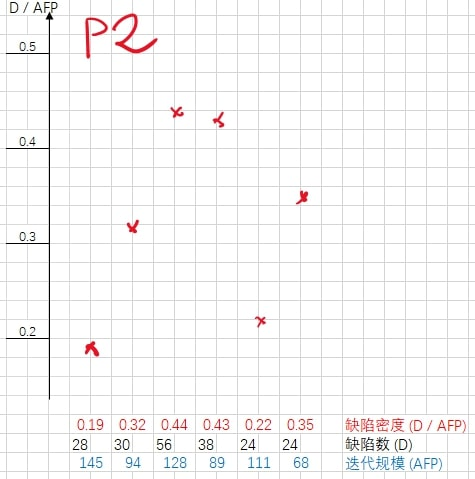
\includegraphics[width=6cm]{P2CcScreenshot_2021-09-25_111304.jpg}
\includegraphics[width=6cm]{P10CcScreenshot_2021-09-25_104057.jpg}

我问:你觉得怎么样?是否稳定?可否建立基线?(希望他可以自己找出答案,不仅仅听我的。)

他说:觉得P10比较好,波动的幅度不大,P2的差异太大了。\\
我说:是的,波动这么大,其实不用画控制图。\\
应先问问P2 项目经理变化这么大(68 -
145)的原因。确保数据正确之后,才可以分析数据,建立基线。其实这些项目数据量都不够。
虽然如此,你还是可以告知两项目组这初步分析结果,但必须要提醒他们数据还未稳定下来。
还记得我们培训时讲过以下基线例子,当过程已经稳定后(没有异常点),
如有异常波动超越了控制图上下线范围,表示过程可能有基本变化。
当变化后的过程稳定下来后,我们便需要更新基线。


\includegraphics[width=6cm]{925BeforeScreenshot_2021-09-25_115004.jpg}
\includegraphics[width=6cm]{925AfterScreenshot_2021-09-25_115237.jpg}

{[}详见附件A3: 如何画ImR控制图{]}

\hypertarget{ux5206ux6790ux9879ux76eeux6570ux636eux5efaux57faux7ebf}{%
\subsection{分析项目数据,建基线}\label{ux5206ux6790ux9879ux76eeux6570ux636eux5efaux57faux7ebf}}

我问过程改进组长: 你们如何得出基线的?有什么分析?\\
答:这个就是我们各项目每个迭代的数据收集表,我就把以往所有项目的每迭代数据,统计所有数据,得出Q1(P25)、Q2(P50)跟Q3(P75)的数,成为我们的基线。\\
问:你有没有分析这些数据?会不会不同的项目之间不一样,导致你的总的基线需要细分一下呢?\\
然后我就举了一个我们用来培训的例子,对70个项目,收集了各种缺陷的统计,我们总体把缺陷归纳成7种类型。如我们按那个7种类型,各自看他的象限图的时候,明显看到他们是之间是有区分的,不能合并成一个基线,如果合并成一个基线,那整个基线的范围就太宽了,没有什么好的参考作用。从最低的0.3左右到最高的0.7。但是如果我们分成7组基线的话,每个基线的范围就窄很多,更有参考作用。\\

\includegraphics[width=10cm]{Opp_3.jpg}

所以我们就简单地依据公司的不同项目,画出各项目的缺陷密度,看看是怎么分布。\\
问:所以你的基线不应该只是看所有的范围,而应该是针对这个稳定的取一个基线,针对这个这两个项目去考虑比较。因为这种比较稳定的项目数据基线,才更有参考作用。加入其它的项目只可能加宽基线范围,对后面项目作参考没有好处。\\
我再问:有了基线以后,你如何依据商业目标去制定你下个月的质量目标?\\
答:从商业目标,我们可以推算出缺陷数或者缺陷密度大概是什么水平?我们统计一下,平均一个缺陷的修复成本是112元左右。所以这个商业目标就可以帮我们知道,从业务目标每个月的缺陷密度要多少才可以有可能最终达到整年的成本降低计划。\\
我说:好啊,有了这个从业务目标得出的质量目标后,你怎么制定改进行动以达到规定成本降低目标?因为如果你没有什么基本的改变,理论上,缺陷密度或者缺陷数是不会降的。\\
我问:你们除了收集数据,有没有把过去每个迭代的质量相关数据标注在生产力发展趋势图上,让你们个人与团队都可以看到过去的变化?如果团队里个人之间的差异很大,这情况可能会按每个人统计更准确。

\hypertarget{ux57faux7ebfux6570ux636eux5206ux6790}{%
\subsection{基线数据分析}\label{ux57faux7ebfux6570ux636eux5206ux6790}}

我说:分析后,可以比较不同项目之间基线范围的差异。
判断项目之间的差异有多大?是否合适归纳成一个总的公司基线。

除了按项目细分,也可以按其他维度细分(例如,按各种缺陷类型的比例。)帮你回答以下问题:

\begin{itemize}
\tightlist
\item
  系统测试 / 验收测试缺陷从前面那个阶段遗漏下来
\item
  代码评审的效率(Yield)
\item
  效率是否跟缺陷种类相关?
\end{itemize}

如果差异很显著,就不需要使用 方差分析(超过2组) , 双样本 T检验
(2组)方法判断分组有没有显著区分。

\hypertarget{ux5229ux7528ux57faux7ebfux4e0eux6a21ux578bux5236ux5b9aux8d28ux91cfux8ba1ux5212}{%
\section{利用基线与模型制定质量计划}\label{ux5229ux7528ux57faux7ebfux4e0eux6a21ux578bux5236ux5b9aux8d28ux91cfux8ba1ux5212}}

要降低最终测试缺陷率,不能单靠不断提醒自己要努力。
要提升,也可以利用80:20原则, 针对占比最多的缺陷类型入手。

我们发现不良分支类占比最多。
过程改进组使用KJ头脑风暴法,找出根本原因,并用加强评测/预防来减少失效质量成本的思路,得出以下对应纠正措施:

\begin{itemize}
\tightlist
\item
  评测

  \begin{itemize}
  \tightlist
  \item
    完善评审检查单,增加与不良分支相关的检查项希望能在评审时检测出来。
  \end{itemize}
\end{itemize}

\begin{itemize}
\tightlist
\item
  预防
\end{itemize}

\begin{description}
\tightlist
\item[]
对应以下四大类根因种类的改进措施:
\end{description}

\begin{enumerate}
\tightlist
\item
  教育/培训 education 编码规范与培训没有明确要求
\item
  个人疏忽 oversight 忽略了要尽量避免不良分支
\item
  执行 transcript 因不良分支不是语法错误,IDE与静态检查代码都没有发现
\item
  团队沟通 Communication 组长安排编程任务与查看代码时没有注意
\end{enumerate}

大家讨论后,除了改善规范检查单与培训外,也决定写个代码扫描小程序来暴露和数代码里这类问题,不仅仅靠人工评审查看。

\begin{description}
\tightlist
\item[]
= = = =
\end{description}

基于从项目收集的数据 - 每一个阶段的缺陷数,返工工作量范围,
过程改进组建立了一个水晶球蒙地卡罗预测模型{[}详见附件A5{]}:
例如对每一个迭代

\begin{itemize}
\tightlist
\item
  输入本迭代动态功能点数(规模)与各过程(需求/设计/编码)的缺陷率(引入多少缺陷)
\item
  输入需求评审各种方法的评审工作量和预估评审效率
\item
  输入设计评审各种方法的评审工作量和预估评审效率
\item
  输入代码评审各种方法的评审工作量和预估评审效率
\item
  输入代码单元测试的缺陷排除率
\item
  输入系统测试的缺陷排除率
\item
  模型便预测系统测试后的遗漏缺陷数,与返工工作量
\end{itemize}

因为要提高评审效率需要花工作量,
这模型就可以帮我们比较:哪个过程,使用什么评审方法,目标的评审效率,对缺陷数和质量成本的效果。

开始的时候,项目经理只能依赖经验来估算,现在有了公司的基线预测模型与性能目标要求作参考,便可以更好地制定本迭代的质量目标(各个过程,包括系统测试要发现多少缺陷
和相关的评审方法)。

无论是基线,或模型都是有它们的局限和不确定性。
所以项目经理会除了参考极限与模型的预测外,还是会依据经验,综合考虑来制定量化目标和选用那种方法。


\includegraphics[width=10cm]{MoveDefectsForwardScreenshot_2021-11-18_215056.jpg}

Key: 蓝色是以往的基线 - 绝大部分缺陷都是在系统测试才发现;
浅绿色是量化质量计划的缺陷率目标 -
参考PPM(红线),计划利用提高前期评审的效率,减少系统测试与验收缺陷密度\\

\framebox{%
\begin{minipage}[t]{0.97\columnwidth}\raggedright
制定质量计划 (Quality Plan)

\begin{itemize}
\tightlist
\item
  从需求到设计、编码,如果方法没有变化,项目质量也不会改变。以代码评审为例,质量计划也要明确什么过程,选择哪一种评审方式。例如一般前端的代码,并非核心,使用简单的一对一或者代码扫描便可以了;但对于一些有逻辑处理的核心模块,可能需要用正式会议评审才能有效地找出大部分缺陷。
\item
  现在回顾复盘不像以前只是讨论哪些缺陷?哪些模块有问题?交给哪个开发去跟踪并处理?
\item
  开发成员看到团队的趋势数据,就会想不断提升,保持和以往一样的同一个水平也不行,现在团队包括每一个成员都会关注质量生产率指标。
\end{itemize}\strut
\end{minipage}}

\hypertarget{ux66f4ux65b0ux91cfux5316ux6027ux80fdux76eeux6807}{%
\section{更新量化性能目标}\label{ux66f4ux65b0ux91cfux5316ux6027ux80fdux76eeux6807}}

我问过程改进组长:还记得六个月前,我问你们的改进目标吗?\\
答:当然记得,要降低开发成本一百万\\
我们刚做了回顾,从项目数据,基线,预测模型,并更新了目标。下图从高层目标关连到研发性能目标QPPO
:\\


\includegraphics[width=10cm]{目标上下关系图.jpg}

我问:挺好,你们如何把高层的业务目标关联到开发团队的性能目标QPPO?\\
答:以前没有太多数据,到了3月份,我们就依据过去6个月的数据得出缺陷密度的基线------Q1:
0.27、Q2: 0.35、Q3: 0.41 (Note1)。依据这个基线,制定4月份的QPPO目标是Q1:
0.25,Q2: 0.34、Q3:
0.47,因为我们觉得中位数应该有些下降,但是不是每一个项目都具备强配合能力,所以估计向下那个范围还是跟以前差不多。\\
::Note1: Q2=中位数 50 percentile,或叫P50 ; Q1= 25 percentile,P25 ; Q3=
75 percentile,P75

制定性能目标除了要有分布范围,例如 Q1 / Q2 / Q3 , 不再是以前升10\%
的那种单点目标:\\
以前单点的话只会说均值从X\%降到Y\%(eg.来年希望降低质量成本25\%)。但不会像这种从Q1、Q2、Q3,不仅考虑中位数也考虑范围。以前单点时可以说,是否达到预期的目标,只看中位数。这种考虑不够全面。现在我们有分布的概念,当被问到预期目标完成情况时,我们会说Q1达不到,跟以前一样,Q3也没有什么变化,但我们Q2
是达到本来预期目标。\\

\hypertarget{ux6539ux8fdbux6548ux679c}{%
\section{改进效果}\label{ux6539ux8fdbux6548ux679c}}

从建立第一轮基线后,过了三个月,过程改进组分析8个试点项目的改进效果,准备汇报给高层,发现8个项目的数据差异还是很大。其中有2个项目很明显看到有质量的提升、系统测试缺陷的降低、返工量的降低。有三个项目数据不全,而且也没看到太大的变化。有两个项目几乎就没有提供数据,过程改进组分析原因,发现和这个项目组的领导有关,两个有效果的项目,他的领导一直积极支持量化管理过程改进。\\
我看过程改进组好像对结果有点失望,就跟大家打打气说:\\
大家千万不要以为过程改进的路很简单,开始的时候反对声音大是很正常的,因为要改变一个人的习惯是很难的,但起码从这几个月的实验数据来看,我们的量化管理是有效果的。后面我们就可以利用这两个项目的经验,开始后面的改进。管理层监督都应该以数据说话,不应该只是听高层管理的一言堂。我相信再过几个月,会有越来越多项目组采用这个方式来加强管理。丰田的大野赖一先生在50年代推动精益管理时,也不是所有的主管听他这一套,但他一直坚持下来。现在不仅丰田,其他的日本汽车公司都以丰田生产方式(Just
in time) 生产汽车,成为世界级的汽车生产流程。\\

\hypertarget{ux603bux7ed3}{%
\subsection{总结}\label{ux603bux7ed3}}

\begin{enumerate}
\tightlist
\item
  单靠统计分析是不会提高开发质量的,必须找到对应的方式,例如注重同行评审,不要等到系统测试才发现缺陷。
\item
  做好需求以减少设计与编码对需求的误解。
\item
  统计数据让开发人员可以``看到''到现在的状态与趋势,且分析新方法对提升有没有作用。
\end{enumerate}

\textbf{这案例主要方法与重点}\\
1.目标要满足SMART\^{} 原则,目标有分布的概念\\
::\^{}(S=具体 M=可度量 A=可实现 R=相关的 T=有时间 )
2.降低质量成本的方法:\\
定期复盘造成本次缺陷最多的原因,是需求原因还是编码过程不规范:从而加强代码评审和规范性检查,还是完善需求评审检查单。

3.质量抓重点:例如一般前端的代码。并非核心,使用简单的一对一评审或者代码扫描便可以了;但对于一些有逻辑处理的核心模块,可能需要用正式会议评审才能有效地找出大部分缺陷

4.检查单可弥补经验的不均衡。

5.收集个人数据\\
主要依赖手工收集,因很多是无法靠系统自动识别的 ,如缺陷源自哪个过程。

6.利用水晶球预测模型,帮项目组在策划时找最佳配搭


\cite{MA2References1}


\PassOptionsToPackage{unicode=true}{hyperref} % options for packages loaded elsewhere
\PassOptionsToPackage{hyphens}{url}
%
\documentclass{book}        % from not too short p76 pagestyle
%\usepackage{fancyhdr}
%\pagestyle{fancy}
%ensure chapter section headngs in lower case
%
\usepackage{graphicx}
\DeclareGraphicsExtensions{.png,.jpg}
\usepackage{xeCJK}
\setCJKmainfont{SimSun}
\usepackage{lmodern}
\usepackage{amssymb,amsmath}
\usepackage{ifxetex,ifluatex}
\usepackage{fixltx2e} % provides \textsubscript
\ifnum 0\ifxetex 1\fi\ifluatex 1\fi=0 % if pdftex
  \usepackage[T1]{fontenc}
  \usepackage[utf8]{inputenc}
  \usepackage{textcomp} % provides euro and other symbols
\else % if luatex or xelatex
  \usepackage{unicode-math}
  \defaultfontfeatures{Ligatures=TeX,Scale=MatchLowercase}
\fi
% use upquote if available, for straight quotes in verbatim environments
\IfFileExists{upquote.sty}{\usepackage{upquote}}{}
% use microtype if available
\IfFileExists{microtype.sty}{%
\usepackage[]{microtype}
\UseMicrotypeSet[protrusion]{basicmath} % disable protrusion for tt fonts
}{}
\IfFileExists{parskip.sty}{%
\usepackage{parskip}
}{% else
\setlength{\parindent}{0pt}
\setlength{\parskip}{6pt plus 2pt minus 1pt}
}
\usepackage{hyperref}
\hypersetup{
            pdfborder={0 0 0},
            breaklinks=true}
\urlstyle{same}  % don't use monospace font for urls
\usepackage{longtable,booktabs}
% Fix footnotes in tables (requires footnote package)
\IfFileExists{footnote.sty}{\usepackage{footnote}\makesavenoteenv{longtable}}{}
\setlength{\emergencystretch}{3em}  % prevent overfull lines
\providecommand{\tightlist}{%
  \setlength{\itemsep}{0pt}\setlength{\parskip}{0pt}}
\setcounter{secnumdepth}{0}
% Redefines (sub)paragraphs to behave more like sections
\ifx\paragraph\undefined\else
\let\oldparagraph\paragraph
\renewcommand{\paragraph}[1]{\oldparagraph{#1}\mbox{}}
\fi
\ifx\subparagraph\undefined\else
\let\oldsubparagraph\subparagraph
\renewcommand{\subparagraph}[1]{\oldsubparagraph{#1}\mbox{}}
\fi

% set default figure placement to htbp
\makeatletter
\def\fps@figure{htbp}
\makeatother
\date{}
\begin{document}               % plus the \end{document} command at the end.

%\includegraphics[width=12cm]{123BookCoverScreenshot_2022-01-23_141507.jpg}\\

%\includegraphics[width=6cm]{赛希咨询.jpg}

\begin{titlepage}\thispagestyle{empty} \vspace*{3em}{\centering\Huge 软件开发过程改进(V01初稿) \par}\clearpage
\newpage \thispagestyle{empty} \mbox{} \cleardoublepage
\thispagestyle{empty} \vspace*{7em}{\centering\Huge 软件开发过程改进\par}{\centering-- 从个人到团队到公司from individual to team to organization \par}\cleardoublepage

%\includegraphics[width=12cm]{123BookCoverScreenshot_2022-01-23_141507.jpg}\\

%\includegraphics[width=6cm]{赛希咨询.jpg}

\thispagestyle{empty} \vspace*{\fill} \parbox{.8\textwidth}{\raggedright \scriptsize
\textit{impossible} publisher 2022

printed blindfolded

design: \LaTeX
}
\end{titlepage}
\clearpage \thispagestyle{empty}\cleardoublepage
\newpage % Make sure the following content is on a new page

%----------------------------------------------------------------------------------------
%	TABLE OF CONTENTS
%----------------------------------------------------------------------------------------

\tableofcontents % Prints the table of contents

%----------------------------------------------------------------------------------------
%	INTRODUCTION SECTION
%----------------------------------------------------------------------------------------

\chapter*{前言 Prologue} % Introduction chapter suppressed from the table of contents

\begin{quote}
We are uncovering better ways of developing software by doing it and helping others do it.\\
--Agile Software Development Manifesto
\end{quote}

当今IT时代,软件开发越来越重要。但如何让软件开发也可以像其他工程领域,可以利用数字化来不断提升呢?\\
不少开发团队已经开始利用敏捷开发,两到四周迭代去对应客户需求不断变化。团队基于每迭代回顾、复盘其实可以利用数据,帮助进一步提升团队的质量与生产率。

本书主要是针对这点,借用一些实际的方法,场景,案例,让理解如何通过演化的过程,使个人到团队不断改善,包括:\\
1.制定方式/步骤/模型\\
2.针对问题的根因做试验\\
3.评判下一轮迭代的效果\\
4.利用数据,团队得到反馈,持续完善过程

这持续完善的过程,以前在工业生产年代已经被证明有效,Deming, Juran, Shewart等质量大师已经验证了这种改进方式,配合数据统计分析,可以提升生产线的质量与生产率。\\
如何利用这方式把作坊式的软件开发逐步变成有序的软件工程?

与工业生产不同,软件开发很多时候都无法像工厂收集到各种数据,但软件工程师仍然可以利用数据反馈做改进。很多软件工程师虽然开发能力很强,但未养成个人收集数据的能力和习惯,也不清楚如何用数据,持续改善。本书针对这些需求,以如何改善软件质量为目标,建议一些具体的做法、工具,帮助个人和团队可以立马尝试走出量化敏捷开发的第一步。

本书主要内容包括:

\begin{itemize}
\tightlist
\item
  从个人如何提升开始
\item
  如何基于个人的提升,演化成团队的提升
\item
  探索背后的一些管理思路,包括:

  \begin{itemize}
  \tightlist
  \item
    德鲁克
  \item
    敏捷开发 与 X-Y理论
  \end{itemize}
\item
  针对敏捷开发,如何利用度量与分析,不断提升质量\\
\end{itemize}


%----------------------------------------------------------------------------------------
%	BOOK PART
%----------------------------------------------------------------------------------------
\part{个人经验分享}我深信要提升必须源自个人,如果团队成员本身没有动力,团队无法提升。我虽然差不多天天都与软件开发团队打交道,但自己编码的时间很少,下面是相关的经验分享。\\


\chapter{个人学习Python编码} % Introduction chapter suppressed from the table of contents

第四天早上10:00我终于把所有功能写完并通过自动单元测试!\\
(老师说学编码必须动手,但我平时忙于工作,这次趁十一长假做编码练习题。上次做题已经是春节后,在集中隔离期间做过两题。这次的练习题只有十个功能,本来预计可两天完成。)

\framebox{%
\begin{minipage}[t]{0.97\columnwidth}\raggedright
练习题 (Problem
Set)------分析美国过去温度变化,提供了美国超过20个城市的每天平均温度。(从1961年到2015年)

\begin{itemize}
\tightlist
\item
  先写基本功能:

  \begin{itemize}
  \tightlist
  \item
    画散点图,回归分析,计算标准差与决定系数 (R\textsuperscript{2} Coef.
    of determination)
  \end{itemize}
\end{itemize}

\begin{itemize}
\tightlist
\item
  分析过去的五六十年数据,来判断美国或全球是否在暖化
\end{itemize}

给学生的文件包:

\begin{enumerate}
\tightlist
\item
  ProblemSet5.pdf : 分成 A、 B 、C、 D、
  E部分,详细说明每部分要开发的功能
\item
  PS5.py 程序模板,学员填入代码
\item
  PS5\_test.py 自动单元测试模块,自动测写好的PS5.py
\end{enumerate}\strut
\end{minipage}}


回顾一下,像我这种Python新手,因为不熟悉Python语言的属性与特性,必须按部就班,一步一步来写,欲速则不达。

更重要是体会到个人如何记录数据并分析:

\framebox{%
\begin{minipage}[t]{0.97\columnwidth}\raggedright
\hypertarget{ux8bb0ux5f55ux65f6ux95f4}{%
\subsubsection{记录时间}\label{ux8bb0ux5f55ux65f6ux95f4}}

十多年前我在美国考CMMI培训师,被观察时,
观察老师会在培训后告诉我,每一个模块用了多少时间,与计划对比。
从此以后每次培训我都会习惯记录每个模块所花的时间。

\hypertarget{ux600eux6837ux505a}{%
\subsubsection{怎样做}\label{ux600eux6837ux505a}}

培训时,我都会在桌上放一数字电子钟,记录每一个模块的开始时间与结束时间。上完一天课,晚上在电子表单计划时间旁边写上每个模块的实际时间。
这三天半,我也是用这种方式记录每个模块的时间。

\hypertarget{ux8bb0ux5f55ux7f3aux9677}{%
\subsubsection{记录缺陷}\label{ux8bb0ux5f55ux7f3aux9677}}

因为每个功能都很小,不到20行, 所以没有正式把缺陷与返工工作量记下来。
尤其是一些小的语法错误问题立马就改正了。
但影响较大的重大缺陷,我会记在模块旁边,算是这个模块花的时间。

个人记录实际时间没有想象中这么困难,
只要每天晚上简单按当天本子的数据更新电子表单,避免遗忘。
%will remove after jpg inserted
\includegraphics[width=12cm]{PspLogScreenshot_2021-10-06_174917.jpg}
\strut
\end{minipage}}



\framebox{%
\begin{minipage}[t]{0.97\columnwidth}\raggedright
\hypertarget{ux56deux987eux5206ux6790}{%
\subsubsection{回顾分析}\label{ux56deux987eux5206ux6790}}

整个编程结束后,写上每一个模块的实际代码行数。注意:如果模块是复用其他模块代码,便需要注明改动的代码行数。例如:evaluate\_models\_on\_testing13行只修改了1行。

分析:除了标准差模块(gen\_std\_devs)以外,其他功能都能在1-3个小时之内完成。

计算标准差的功能花了 10
小时,问题出在我编码时没有详细看需求。开始以为是求每个城市的温度标准差。
然后再求标准差的平均数。\\
测试不通过后,
也没有再看需求便假定求当年几个城市所有当年每天温度的标准差,还是不对。
到了第四天早上再看看 ProblemSet5.pdf
需求描述才知道我一直误解了这功能需求。

\texttt{gen\_std\_devs~~对应每一输入年份,返回一个数值,依据以下计算:}~\\
\texttt{~1)按输入的所有城市,计算当年每一天的平均温度(所有城市的平均)}~\\
\texttt{~2)计算当年每一天平均温度的标准差}~\\

所以如按我本来的算法,算一个城市是正确,但两个或者多个城市的时候,答案就比正确答案大。

针对这个计算标准差问题,一直以为是语法问题公式计算错误问题。
但我用一些简单的数据检验去,未能发现任何不正常。
来来去去都没有实际的进展,差点想放弃。

\hypertarget{ux7ecfux9a8cux6559ux8bad}{%
\subsubsection{经验教训}\label{ux7ecfux9a8cux6559ux8bad}}

我常常跟客户说,要做好需求评审,才能降低返工工作量。 这次编码实验的经验告诉我,如果前期过程有缺陷遗漏, 后面确实要付出很大的代价。(10小时返工工作量是评审平均2小时(1 - 3小时)的5倍,这案例还只是15行代码的小功能。在实际软件开发项目中,经验丰富的编码员应不像我这么笨,但估计因前面过程遗漏缺陷在系统集成后,测试才发现的返工量应也不止5倍!)

有了数据记录,这类宝贵个人经验便可以转化为改进(不仅仅是一个印象)。例如,可以把这些变成个人风险清单的检查项 
-\/-避免同类问题再发生。

\hypertarget{ux7ed3ux8bba}{%
\subsubsection{结论}\label{ux7ed3ux8bba}}

统计工作量与缺陷数据要从个人开始,并在回顾分析各种缺陷类型的返工量,找根因,制定对应措施,下次可以避免同类缺陷,我们才有动力继续收集数据。\strut
\end{minipage}}


\hypertarget{ux5176ux4ed6ux7f16ux7801ux7ecfux9a8cux6559ux8bad}{%
\subsection{其他编码经验教训}\label{ux5176ux4ed6ux7f16ux7801ux7ecfux9a8cux6559ux8bad}}

\begin{itemize}
\tightlist
\item
  最佳实践: 尽量用最小的行数完成功能

  \begin{itemize}
  \tightlist
  \item
    像Python这类成熟的语言,绝大部分的功能都已经具备
  \item
    尽量避免基础方法编写一个已有的功能(reinvent the
    wheel),除了耗费时间外,还会写多错多
  \end{itemize}
\end{itemize}

\begin{itemize}
\tightlist
\item
  写任何程序前必须先有自动化测试用例

  \begin{itemize}
  \tightlist
  \item
    虽然自己可以先想一些数据自己简单测一下
  \item
    但替代不了另外一个人写的测试用例。跑通才有信心程序正确
    (所以自动单元测试是使用最多的程序)
  \end{itemize}
\end{itemize}

\begin{itemize}
\tightlist
\item
  架构与设计很重要

  \begin{itemize}
  \tightlist
  \item
    校方除了提供测试脚本外,还提供了写程序的模板 (PS5.py)
  \item
    每个功能都明确,输入是什么,什么数据类型,输出是什么
  \item
    学员自己只需要填写实现的代码部分
  \end{itemize}
\end{itemize}

\begin{itemize}
\tightlist
\item
  先把握好新功能的用法与结果

  \begin{itemize}
  \tightlist
  \item
    前面发现不少缺陷,是因为不清楚某功能的用法
  \item
    在写代码之前,自己应开个沙盘,用小程序先试验一下这计算功能有什么参数,会出什么结果
  \end{itemize}
\end{itemize}

\begin{itemize}
\tightlist
\item
  先评审后测试

  \begin{itemize}
  \tightlist
  \item
    在跑程序之前,屏幕展示或打印出刚写好的代码,用铅笔在白纸上按程序的逻辑,从头思考一下每个数据的种类和中间的变化
  \item
    盲目地去跑程序或测试,最终只得出测试失败,但还不清楚错在哪里,如何修改。所以不如在跑程序或测试前,自己先动脑筋模拟一次,仔细想通每个数据的变化
  \end{itemize}
\end{itemize}



\chapter[克服拖延症]{锻炼高效: 克服拖延症}  % Introduction chapter suppressed from the table of contents

有位北京的技术总监问:现在我遇到最大的难题就是如何提升下面技术人员的能力,如果他们全都是高手,我就很轻松了,但实际上最多只有三分之一,其他都是中低水平。您接触过这么多软件开发团队,有什么好方案?\\
我说:我没有解决提升技术人员能力的银弹,但你可以听听我最近这故事:\\
:: = = = = = = = = = = = = = = = = = = = = =

\includegraphics[width=8cm]{小李图.jpg}

小李:你能够在一周内写完程序通过测试,并把整件事汇总成分享文章初稿发布很厉害呀。\\
我:其实你也可以做到。在《个人写程序并记录统计的一些经验分享》里,我只是写了与软件工程相关的重点,
但个人有没有高效率的习惯其实更重要。

我在五年前教授项目管理时参考过一本效率小册 {[}详见 Reference1{]},
这本小册罗列了99个小技巧,每个技巧都不超过一页纸,我自己也一直用这小手册提醒自己。

\includegraphics[width=10cm]{超效率目录.jpg}

例如,第一章``克服拖延症'',这里的几乎全部技巧有帮助:\\

\begin{itemize}
\tightlist
\item
  周 / 日目标 (1 Weekly / daily Goals)
\end{itemize}

\framebox{%
\begin{minipage}[t]{0.97\columnwidth}\raggedright
我每天都会定计划,早上希望完成哪些功能,下午完成哪些。当然这个计划也会按实际的进展调整。

周 /
日目标是个人时间管理的基本功。每一天第一件事不是回邮件,而是仔细想想今天要完成什么任务,每一周的开始,也应该想我本周希望完成什么任务。不然的话,每天的时间就很容易被琐碎的小事吃掉,一事无成。\\
\strut
\end{minipage}}

\framebox{%
\begin{minipage}[t]{0.97\columnwidth}\raggedright
背后的道理很简单, 要把时间花在重要、但非紧急的活动(下图右上角
)上,效率才会出来。

\includegraphics[width=10cm]{pfjp30.jpg}

\hypertarget{ux9650ux5b9aux65f6ux95f4-2-timeboxing}{%
\subsubsection{限定时间 (2
Timeboxing)}\label{ux9650ux5b9aux65f6ux95f4-2-timeboxing}}

把每天的任务安排成时间段,每一段不应超过1.5 小时。\\
一般人可以专心集中的时间段都不会超过60分钟,小孩可能就更短。如果老师叫你星期五5点钟交卷,你不会3、4点就交,都会等到最后十分钟,甚至五分钟。所以如果我们把一天的时间切开成
1 ~ 1.5 小时时间段,自然有动力, 希望在时间之内完成任务。\\
我们写代码的时候应该也是用同样的原理。例如。前面那个总共花了10个小时的功能,也是本身尝试了很多次。每次当我发现超过了1小时或者1.5
小时,我就会把它放下来,先做其他事。

\hypertarget{ux5206ux89e3ux4efbux52a1-3-dissolving-tasks}{%
\subsubsection{分解任务 (3 Dissolving
tasks)}\label{ux5206ux89e3ux4efbux52a1-3-dissolving-tasks}}

因为都是练习题,所以每一个功能都比较细,不会超过二十行。如果我们平常做开发时,也必须要把一些大、复杂的功能预先拆分成小的功能才有效率。\strut
\end{minipage}}

\hypertarget{ux52a0ux5f3aux81eaux5f8b-6-building-self-discipline-muscles-ux6668ux793c30-morning-rituals-ux65e5ux5e38ux8fd0ux52a8-32-make-an-exercise-routine}{%
\subsubsection{加强自律 (6 Building Self-Discipline Muscles), 晨礼(30
Morning Rituals) 日常运动 (32 Make an Exercise
Routine)}\label{ux52a0ux5f3aux81eaux5f8b-6-building-self-discipline-muscles-ux6668ux793c30-morning-rituals-ux65e5ux5e38ux8fd0ux52a8-32-make-an-exercise-routine}}

不要以为编码是一个单纯的脑力活。整天坐在电脑前面敲代码就可以,如果人的体力、精力没有配合上也会出问题,好在我每天早上一直坚持三十到四十分钟的轻量运动,然后晚饭前半个小时到一个小时的骑单车或者慢跑的习惯。中间也是不是整天坐着,一段时间会走一走,喝橙汁等,确保身体不断在动,才不会困,保持动力。

贝多芬每天都会去外面散步,来启发一些创作的灵感,然后他会立马把这些写在本子上,用于后面的音乐创作。早上的跑步也可以让我有多些创作灵感。

\hypertarget{ux4e0dux4f1aux5206ux5fc3ux7684ux5de5ux4f5cux573aux6240-11-create-a-distraction-free-workplace}{%
\subsubsection{不会分心的工作场所 (11 Create a Distraction-Free
workplace)}\label{ux4e0dux4f1aux5206ux5fc3ux7684ux5de5ux4f5cux573aux6240-11-create-a-distraction-free-workplace}}

\hypertarget{ux8f7bux7b56ux5212ux8fedux4ee3ux518dux7b56ux5212-13-ready-fire-aim}{%
\subsubsection{轻策划,迭代,再策划 (13 Ready , Fire,
Aim!)}\label{ux8f7bux7b56ux5212ux8fedux4ee3ux518dux7b56ux5212-13-ready-fire-aim}}

三十年前,软件开发都是很大型的一些项目,整个架构要设计好才动手去写代码。现在反过来,需求变化极大,开发都需要敏捷,轻文档轻计划。尽快写好代码,做一些功能给客户,从反馈优化下一轮。我这次的几天开发也是用同样原则,没有花时间在一些设计或者文档。想直接把那个代码写出来,并通过单元测试,就节省很多耗时间的工作。把有限的时间都放在写好代码上。

\hypertarget{ux4e0dux65adux6e05ux6d17-10-churning}{%
\subsubsection{不断清洗 (10
Churning)}\label{ux4e0dux65adux6e05ux6d17-10-churning}}

万事开头难。我在开始的半天也是遇到同样问题,不知如何入手,太久没看写代码的书了,很多基本的都不知如何入手。所以我开始的时候不会直接尝试写题目里面的功能,而是重写一些书本的代码,看看跑出来怎么样,然后逐步提升。写一些基本功能,慢慢有了习惯,调整过来了,后面就越来越顺。好比一台旧的水泵,刚开始抽上来的水总是有难喝的铁锈,只要不停止抽水,当污水最终都从系统中抽出后,就能发现底下的净水。

\hypertarget{ux8981ux6709ux597dux7684ux571fux58e4-8-remove-your-hidden-roadblocks}{%
\subsubsection{要有好的土壤 (8 Remove your Hidden
Roadblocks)}\label{ux8981ux6709ux597dux7684ux571fux58e4-8-remove-your-hidden-roadblocks}}

在含盐量高的土壤里种植物,是结不出果实的。浇水、平衡在阴凉处和阳光下的时间都抵不过根部吸入的毒素。如果我们没有积极性,就可能是土壤的问题。如果没有足够的积极动力,就不会在长假专注写程序,也不会定期要求自己写分享文章。所以要有明确/很想达到的目标驱动。
像一个作曲家,他希望写出很多经典的优秀作品,不满足于现在的状态。觉得自己的灵感或者创造力没有发挥出来,成为可以保留下来的东西。也是这种驱动力让我可以一直努力做这件事。\\

\hypertarget{ux6452ux5f03ux62d6ux5ef6ux6076ux4e60-14-quit-your-procrastination-vices}{%
\subsubsection{摒弃拖延恶习 (14 Quit your Procrastination
Vices)}\label{ux6452ux5f03ux62d6ux5ef6ux6076ux4e60-14-quit-your-procrastination-vices}}

长假里,大部分人都会把时间用于看视频或电视剧,而我正好没有这个习惯,也一直没有玩网络游戏的习惯,否则肯定完成不了。

最终我用日程记录(91
Timelogging),把整件事和什么活动、时间花在什么地方都记录下来了。

小李:我看你上面列出的技巧,我大部分都还没做到。

我:不要紧,我六年前刚开始定期写文章时情况跟你类似,但只要不放弃,一直往既定目标努力,不良习惯都改正过来了。

我常常说人的潜力是极大的。 舒伯特你听过吗?\\
小李:好像是一个很有名的作曲家。\\
我:是的,但他很年轻31岁(1828)
就去世了,你猜他一生一共写了多少首歌和音乐作品。\\
小李:我记得中学时,老师介绍过他的艺术歌曲,如``鳟鱼 The
Trout'',但他31岁就死了,我猜100 - 200 首歌?\\
我:他一生写了超过460首歌曲(时长\textgreater{}24小时)。除了歌曲,他还写了其他作品,如9首交响曲,20
室内乐,120 钢琴曲等等,每一类都包括大量经典作品,对后世影响深远。\\
小李:如果粗算他一生600作品,算他有16年时间作曲,平均每月要完成3个作品,真是不得了。\\
我:虽然他的作品有大有小(从一首歌,到45分钟的交响曲),他确实生产率极高,而且他最后的7年一直身体都不好,所以他那个时候肯定不会像我们现代996方式工作。
他每天主要是早上用来写作,傍晚便去休息散步。但他会同时做多个创作项目 -
那些项目没有灵感,就暂时放下来,创作其他作品。
他著名的未完成交响曲就是个好例子,只有两个乐章(一般交响曲都是四个乐章)
所以他是使用高效技巧的一个成功例子。

每个人都有自己的理想,但如果没有高效率来执行,理想只是天马行空,天方夜谭,不会有任何成就。有没有疑问?

小李:没有,挺好的,我后面立马就开始。\\

总监说:我大概懂你的意思了,要提升技术人员的能力先要改变他们的习惯,有良好的习惯(如时间管理),才有机会提升。\\
我:是的。\\
总监问:从管理者的角度,我们有什么可以做的?\\

\hypertarget{ux5373ux65f6ux7b14ux8bb0-17-the-capture-device}{%
\subsubsection{即时笔记 (17 The Capture
Device)}\label{ux5373ux65f6ux7b14ux8bb0-17-the-capture-device}}

总监边听边在本子上记下那些重点。高效的人都会有工具帮他记录想到灵感、想法、项目、待做事项等等,不会仅仅靠大脑记忆。你提出一个要求,他会立马写在小本子上,你会觉得他应该会按你要求去处理,但反过来他只是口头说会处理,你会担心很可能没有下文。但我看有些领导,身边只拿个手机,除非他们的记忆力超人,不然话我估计他每天都会忘记不少重要事项。

下一篇,我们将讨论如何从个人上升到团队的提升。\\

\hypertarget{ux676dux5ddeux9ad8ux7ea7ux7ecfux7406ux53cdux9988}{%
\section{杭州高级经理反馈}\label{ux676dux5ddeux9ad8ux7ea7ux7ecfux7406ux53cdux9988}}

人一定要自律!您说的小技巧确实能起到很大帮助,而且我基本都会使用,但如果不养成习惯,想起来使用下,最终还是改不了拖延症,所以要解决拖延症,一定从根源做起,还是得靠自己,需要培养自己意志力、专注力,坚持好习惯,改掉坏毛病。\\

\cite{prod1References1}
 %from individual to team
\chapter[从个人到团队]{锻炼高效: 从个人到团队} 

个人精力有限,必须借用团队才能成倍提高生产率。但不能仅靠组长个人的努力:例如有些开发技术出身的组长,自我时间控制很好,技术也不错,但不懂如何有效下放工作,协助团队成员,导致团队不懂,做不出来,最后组长就自己动手搞定,恶性循环。
所以团队要有效率,除了依赖个人能力外,还需要了解高效团队的挑战。

\framebox{%
\begin{minipage}[t]{0.97\columnwidth}\raggedright
知识工厂 (Knowledge Factory)

一位老同学在东莞有一个"知识工厂",主要是为美国客户服务,输入扫描件,输出修正好的、正确的英文文件。\\
因为美国的人工费用很高,所以客户愿意把一些耗费人力的手工工作外包。\\
虽然公司可以利用识别英文字的软件把扫描件转化成电子版,但只能做到大部分,还是有很多地方需要看原文,手工输入、修正。这个知识工厂就是找一些初中学历的人,经过简单培训后上岗,把编辑好的文档发回给美国客户。一般是按字数收钱,因为是外包业务,利润非常低,所以必须要控制生产效率------如果效率低工厂就不赚钱了。但效率不仅仅是速度,如果有太多错误,客户便不满意,所以也要控制质量。\\
\textbf{典型客户}:\\
*某网站服务,收集了大量老资料,专门帮助美国人寻根。

\begin{itemize}
\tightlist
\item
  例如某美国人可能前几代是从爱尔兰过来,但只知道是哪年哪月,他可以从这网站搜索某时间段轮船的客户名单,所以这公司便需要把大量老轮船客户名单,转换成电子文件,其中也会遇到很多古老的字,扫描软件难以识别。
\end{itemize}

有一天他邀请我去参观东莞分厂,办公大厅里有很多人,大家头戴耳机在屏幕前敲打键盘。\\
员工每 7 - 10
人分成一个小组,每组一个组长,每组头上有个大屏幕,显示着数字。\\
我就问同学这是干什么的,他说这些就是反应每个小组当前的速度,每个组员都可以看到,效果就是让成员们能直观看到工作的反馈:现在整个组的速度、质量如何,都可以从那些数字简单地反映出来。\\
我老同学说:\\
``每个员工和团队都很清楚当前的效率和质量。
从这么多年数据显示,一般新员工经过培训后开始 1 分钟是 55- 85 WPM(Word
per Minute )。
但因为经验少,所以一般错误率比较高。经过几个月的实际工作,速度和准确率都会有提升。我们提拔组长也主要是看他过去的指标是否领先。\\
除了监控,我们也会完善一下新的系统来帮助团队,例如,系统会同步给他们一些提示,也会用语英语读出来,帮助他们更好完成任务。``\\
\strut
\end{minipage}}

以上是团队如何利用系统,提高生产率和质量,让公司盈利生存的例子。
我立马想到,如果没有及时的数字反馈,很难让团队知道自己现在的状态。这跟我每天早上跑步一样,如果没有计时,就没有动力保持或超越以前的速度。\\
克服拖延症里面提过的效率小手册第二章里的“做事要有条理” (Becoming Organized)
如果个人无法把所有所做的事情清晰地分解,就很难有效率。比如,小手册提了几点简单的组织系统帮我们:

\begin{enumerate}
\tightlist
\item
  分成项目 (20 Projects)
\item
  项目由任务组成 (21 Tasks)
\item
  任务或活动,要有开始日期,结束日期 (22 Events)
\item
  分支法 (24 Branch)
\end{enumerate}

一个人要管理一个团队,当那些任务不是仅仅是自己看和做,而是要分摊到团队其他人去完成的时候,就更需要有个系统,让大家看到计划与实际。在项目管理来讲,这个叫工作任务分解
(Work Breakdown Structure WBS)。

我在北京给一家公司做评审时,问他怎么管理项目,他很自信的说跟你上次见不一样了,我们现在有项目管理系统。

其实他说的管理系统只是一个任务管理系统(类似缺陷管理,每一个缺陷或任务独立,然后就让成员填写任务的完成情况)。因为系统只能跟踪任务的实际完成情况,没有WBS分解能力,难以管理整个项目。可以想象,如果项目有一百多个任务,经理怎么知道任务的进展情况呢?只能看到每个任务状态。但是如果能把任务按过程(如测试,编码),模块(如
A模块、B模块等)或迭代分组,我就可以把那100多个任务汇总成5、6个组,经理或团员就可以从系统中得知项目的情况。

:= = = = =\\

某家做保险系统的国际公司,因为要控制人手,所以采用了外包模式,让顾问公司提供人员来现场做开发,公司内的项目经理手下可能有五、六十人在工作。
以前,他要监控这些开发活动时,需要去检查每个人的情况,忙不过来。
这就可以用一个 WBS 管理的系统,来全局监控开发的情况。
WBS项目管理系统如何帮到这个项目经理呢?
项目管理系统要求每个任务(或工作包)都需要有产出物,而且产出物必须通过评审才算百分之百完成。这样的话项目经理就不需要逐个产出物自己查看了,他可以安排团队自己相互评审产出物,项目经理就可以总体监控项目进展,提高团队效率。\\

:= = = = = =

有些高层也了解项目管理有不足,但觉得是流程的问题,要求先把流程建好,才上自动化系统。这种思路听起来很有道理,但实际上行不通。

原因是过程跟系统是息息相关的,如果没有系统,你的过程只是基于一堆手工模板,无法操作,就好比你可以用excel表希望做项目管理系统一样。原因是那些excel表它不是一个系统,最大的问题是它可以随时更改结果,所以这种系统出来的报告,都是说没有偏差。对监控项目没有作用。
我们后面就用一个实例看看怎么在开始的时候可以尽快尝试一下怎么用一些系统来帮我们管理个人的小项目,因为我们说所有过程改进都应该先从小的试点开始。

现在我们都流行用SaaS系统(Software as a
Service),所以很多服务都可以在线上直接使用,不需要预先安装服务器,数据库,应用软件,配置等等。比如我随便进一个这类的WBS项目管理系统,我输入这两周主要的一些主要活动,如:

\begin{itemize}
\tightlist
\item
  用水晶球完善预测模型
\item
  完善国际功能点教材与资料
\item
  为简化功能点准备一套资料,让公司可以开始使用
\end{itemize}


\includegraphics[width=10cm]{微信截图_20211029132308.jpg}

因为我都在外面忙,我只是可以把这些重点设出来。然后每天会议要求做的人在里面添加活动:

\includegraphics[width=10cm]{微信截图_20211029090316.jpg}

因为它是一个SaaS系统,所有团队的成员不一定是在同一个办公地点,都可以看到,还可以上传任务的产出物,并看到任务的完成百分比。

每周五,各人在系统填写实际工时(注意:在她填写实际工时的时候,能看到每活动的计划工时):


\includegraphics[width=10cm]{微信截图_20211029090520.jpg}

在没有做这个之前,我也尝试过在大白纸上面每人写上当天和每周的活动,要团队每天下班拍照发我,但发现一点用都没有:

\begin{enumerate}
\tightlist
\item
  我没时间去看里面有没有具体的时间、工作量
\item
  缺乏数字性记录
\end{enumerate}

我开始用这个系统后,两个月过去,就可以有一些统计数据,从系统里面可以抓出来团队或者个人在过去这个时间完成了什么任务,因为都在系统有记录,也因为有产出物,我用Wiki
跟踪这些产出物的话,我就可以在 Wiki
里面记录每一个产出物的缺陷,所以也可以得到每个人或者团队的质量。把本来只是我个人的管理,扩大到团队管理。


 %
\part{再读德鲁克与 X-Y 理论}要提升软件开发质量与生产率,敏捷开发不是必赢的灵丹妙药,有人说敏捷就是精益(LEAN),虽然LEAN是敏捷的重要部分,但不是全部。想要合适地使用敏捷帮助团队提升,便要先了解敏捷开发背后的管理思路。\\

从50年代起,管理学开始探索如何能提高员工的生产率和质量, 发现传统的军队式管理,和工厂式生产线模式不再合适, 提出要让团队自主,管理者要抛开家长式管理的思维,提出X-Y理论。\\

从60年代到90年代,各行各业不少公司,如服务页(酒店),生产等,采用这新思维,取得显著效果。 2000年,17敏捷领结大师,觉得当时美国软件开发有很多严重问题,提出敏捷宣言, 其实背后的管理思路已经有五六十年历史, 下面我们先从现代管理学大师德鲁克先生的一些文章开始, 然后借用我一些教敏捷ACP 用的故事,介绍X-Y理论与敏捷开发的思路。\\

如果读者想多了解敏捷开发,可参考附件 ‘Agile Primer’。 \\
\chapter[如何提升生产率]{再读德鲁克: 如何提升生产率} % Introduction chapter suppressed from the table of contents

\framebox{%
\begin{minipage}[t]{0.97\columnwidth}\raggedright
一家500人的北京IT公司,专门做企业大数据服务。为了加强管理,他们利用项目管理系统做项目挣值分析(Earned
Value),要求团队先做预算,然后按项目任务完成情况报工,监控实际与计划对比。这就是典型传统会计成本监控。监控已发生的任务,但无法帮我们避免一些可能发生的风险。\\
我问技术总监:``你们公司的核心竞争力是什么?''\\
答:``我们的开发团队都很有经验,开发质量也满足客户要求。''\\
问:``你们如何衡量开发团队的质量和生产率?''\\
答:``我们半年前开始利用项目管理系统,每个月按照项目是否有超时或超出预算。''\\
问:``生产率不等同于项目是否延期,其实与同行相比,你们已经算不错,很多其他企业连这些项目基本监控都缺乏,但如果你们也衡量软件开发团队的生产率和质量,你们会更清楚自己是在什么水平?是否在进步?如果你们有团队的生产率和质量数据,你便更好监控项目,可以从团队的生产率和质量数据预测项目可否按期完成。''\strut
\end{minipage}}

如果我们想知道有什么好方式帮助软件开发团队提升生产率,可先回看上世纪人们如何提升工业生产率。

在20世纪初,科学管理的先行者泰勒(Frederic TAYLOR)
先生开始对劳动者做任务分析和管理,研究各个制造业工人的工作,记录劳动者每个动作,和完成动作的体力和时间,研究如何去除多余的动作。

他的结论是:无论什么工作,都是重复性,如果把那些步骤写下来,任何人不需要什么特别训练,熟练后都可以成为一流大师。\\
当时他的理论被不少美国工会强烈攻击,很简单,当时很多兵工厂都有工会,学徒制,要入行必须当多少年学徒,还也要有熟人推荐才进得来。为什么这么刁难,原因很简单,如果你可以最后当成那些兵工厂的领班或工人,你的薪水可能比医生还高。\\
可能是这个原因,二战时,希特勒在日本偷袭珍珠港以后,错误地认为美国不能在短间可以追得上德国的工业化程度,他就决定跟美国宣战,(宣战前美国,因有内战痛苦经历,国内反战声音巨大,导致在一战时几乎都没有参战,不重视发展军工,缺乏军工方面的人才,比如缺乏军用设备(如光学、镜片)的专业技工)。但事与愿违,美国借用了泰勒先生那一套方式,快速建立兵工厂,大量生产飞机、坦克等等设备,生产力后来居上,超越了德国、日本,最终获得二战胜利。\\
20世纪,制造业的体力劳动者生产率增长了50倍{[}2{]},但现在大部分已发展国家,传统的工业生产只占总生产的小部分,大部分是服务业或知识工作。

所以在21世纪,我们的新挑战是如何能同样提高知识工作者的生产率。

\hypertarget{ux4efbux52a1ux662fux4ec0ux4e48-define-the-task}{%
\subsection{任务是什么 (Define the
Task)}\label{ux4efbux52a1ux662fux4ec0ux4e48-define-the-task}}

知识工作与体力劳动不同,知识工作者的工作大都不是预先安排好。比如汽车生产线,工人只需要按照程序安装组件就可以,劳动者只问``怎样做才能做得最好?''。但知识工作中,知识工作者主要问``任务是什么?''。

\framebox{%
\begin{minipage}[t]{0.97\columnwidth}\raggedright
100多年前,20世纪初,当时没有互联网,没有电商。如果你不想亲自去百货公司买东西,你可以把钱寄到百货公司邮购,但这需要很多人手数寄来的现金。当时"SEARS"百货公司,
不采用传统的数钱方式,用磅来称寄来邮购信件有多重,从而判断里面有多少硬币,多少钱,连信封也不打开。这种方式就可以大大减少所需的人手,在短短两年间,把这一块服务的生产率提高十倍。\strut
\end{minipage}}

如果保险公司也问:``任务是什么?''
答案应是``对死亡申请赔偿要尽快,也最省钱。''

\framebox{%
\begin{minipage}[t]{0.97\columnwidth}\raggedright
保险公司本来每次有事发生,客户要补偿时,保险公司传统都要检查三十个以上不同条件。\\
为了增加生产率,保险公司决定只检查以下关键4项:\\
一、这个保险单是否还有效?\\
二、他申请的金额是否与合同匹配?\\
三、那个人名跟那个死亡证是否对应?\\
四、受保人是否对应?\\
最终把本来要平均十五分钟的事情减到三分钟。

现在很多保险公司只对百分之二的抽样做控制,i.e.只对五十分之一的索偿完整地检查所有项,其他都是按上面这种快速方式处理。\strut
\end{minipage}}

医院也可以利用问``我的任务是什么?''这个问题来提高服务的生产率。很多医院花很多时间要求本人填写的资料,进医院前。甚至有些病人,急诊的病人,因为他们可能已经不清醒,无法填写很详细的表格。如果我们用刚才那个问题,这答案是,入院的手续最重要的是希望识别病人的姓名、性别、年龄、地址和如何收费?就是在一个病人,他的门卡上面有的信息。用这个方式可以大大简化入院服务,生产率也自然提高。

所以在服务业我们要增加生产率,最重要不是像以前劳动工人那种看他每个步骤,更重要的是你要想你的任务是什么?\\

\hypertarget{ux4e13ux5fc3ux5de5ux4f5cconcentrate-on-the-task}{%
\subsection{专心工作(Concentrate on the
Task)}\label{ux4e13ux5fc3ux5de5ux4f5cconcentrate-on-the-task}}

另外一个常常影响服务生产率的问题是不能专心集中工作,例如很多医院都说缺护士,但其实每年都有不少的新毕业员工加入,病人也没有大量增加,为什么会人手不够呢?\\
其实很多浪费是由于护士不是做本职工作``护理病人`,而是花了大部分时间在填写报告,而非医护工作。\\

高校老师也一样,主要任务本应是教学生,但其实花了很多时间开会,例如一些委员会会议。\\
销售人员也一样,不是专注与客户沟通,而是花很多时间在无谓的内部会议,填写报告。很多销售员,平均每天起码花不低于三分之一的时间在这类客服工作,跟销售无关。\\
所以每个行业服务人员都应该问这个问题:``我们受聘主要是要干什么的?我们这个工作主要提供什么价值?''\\
比如某百货公司,员工的回应是``销售''。但其他百货公司,可能是"客服"。所以针对不同的目标,公司应该回顾整个团队是否花了很多时间做一些没有价值的工作。\\

\hypertarget{ux4e0dux80fdux5355ux770bux6570ux91cfux8d28ux91cfux540cux6837ux91cdux8981define-performance}{%
\subsection{不能单看数量,质量同样重要(Define
Performance)}\label{ux4e0dux80fdux5355ux770bux6570ux91cfux8d28ux91cfux540cux6837ux91cdux8981define-performance}}

除了问工作是什么以外,也要问怎么做才有效?

比如一个建筑绘图员,不仅仅衡量图的数量,也要取决于他绘图的质量。其他服务,无论是工程、银行、医院、报社也一样。

例如,药厂实验室科学家,质量最重要,数量其次:如果能研发一个一年销售50亿的``明星''药品,肯定比一年发明超过50个`一般'药品
(年销售2000\textasciitilde{}3000万)好。

\hypertarget{ux56e2ux961fux6709ux81eaux4e3bux6743ux81eaux6211ux7ba1ux7406partnership-with-the-people}{%
\subsection{团队有自主权,自我管理(Partnership with the
People)}\label{ux56e2ux961fux6709ux81eaux4e3bux6743ux81eaux6211ux7ba1ux7406partnership-with-the-people}}

1.定义任务\\
2.专注\\
3.定义性能质量\\
如果我们能一步步完善以上三点,就应该不难,与上一个世纪一样,大大提高服务的生产力。

以上3点能否有效,取决于管理者能否把知识工作者当成``资产'',而不是``成本''。

不能再像以前,把工人只是当作一双手,知识工作者要与前线人员团队合作,才有效。有不少公司,比如IBM一直都有已经采取这种方式多年。日本的工业也一样,本来企业家以为可以继续用二战前那种专制的管理方式,但引起很多罢工,后面也改了。在以前工业生产时代,管理者与前线团队互相合作,支持他们只是一种最佳实践,但现代,这是唯一的方式。

\hypertarget{ux5b66ux4e60ux73afux5883learning-environment}{%
\subsection{学习环境(Learning
Environment)}\label{ux5b66ux4e60ux73afux5883learning-environment}}

管理者要支撑支持前线人员组成自主团队。让他们不断改善服务,达到目标。现代,业务环境快速变化,服务人员也要终身学习才跟得上。培训只是开头,更重要的是他们如何把学到的用于工作中。如果每个人都当内部讲师,不仅仅其他员工受益,讲师本身也受益,进步。比如,找某明星销售人员,让他在全国的年会分享成功经验,教大家怎么做好市场工作,培训过程中,他自己也会思考那些是成功要素,更进步。

\hypertarget{ux5bf9ux8f6fux4ef6ux5f00ux53d1ux7684ux542fux53d1}{%
\subsection{对软件开发的启发}\label{ux5bf9ux8f6fux4ef6ux5f00ux53d1ux7684ux542fux53d1}}

你觉得以上德鲁克先生在1991年针对如何提升知识工作者生产率{[}1{]}的建议,适用于软件开发吗?
下面每一点看看:

\hypertarget{ux4efbux52a1ux662fux4ec0ux4e48}{%
\subsubsection{任务是什么}\label{ux4efbux52a1ux662fux4ec0ux4e48}}

上面的例子:处理保险申报、百货公司邮购等,都是精益(Lean)概念,把有限精力放在最有价值的东西,减少浪费。
2000年,17位软件开发大师针对软件开发问题,如项目延期、失败等问题,发表了敏捷宣言,包括:

\begin{itemize}
\tightlist
\item
  不浪费时间写一些对客户没价值的文档,专心写好代码。
\item
  不浪费时间做一个三个月的详细项目计划。而集中精力把后面两周可以做到什么详细计划好。
\item
  每一轮两周冲刺后,与客户沟通,得到反馈才知道哪些开发出来的是对客户有价值,哪些不是客户要到便立马停止。不像以前等到整个瀑布式开发,最终交付才知道。
\item
  极限编程(eXtreme
  Programming,敏捷的一种)提倡测试驱动开发TDD,道理也一样,如果你这个小程序模块,没测试好就集成到整个系统中,后面会产生很多无谓的返工,必须每个模块都先测试好。
\end{itemize}

这些背后都是精益,越来越多软件研发项目使用敏捷开发。\\

\hypertarget{ux4e13ux5fc3ux5de5ux4f5cux4e0dux5206ux5fc3}{%
\subsubsection{专心工作,不分心}\label{ux4e13ux5fc3ux5de5ux4f5cux4e0dux5206ux5fc3}}

最近周末抽空编写Python小程序。\\
但因很久没编码了,所以一天能完成的程序不多,几十行代码。但发现编写程序需要很高的专注力,原因很简单,写文章就算有错别字人家还可以看得懂,但写程序错了一个字就跑不通了。所以我每写一段代码都会依据TDD原则,写十来行就用一个小模块就去测试。这样才可按计划完成当天要完成的练习题。\\
所以不要分心这点在软件开发特别重要。\\
但很多开发人员都要同时兼顾4-5个项目,还要维护一些老项目的出厂后的缺陷,其中有些更要紧急处理。可想象这些开发人员如何能专心写好程序?但不专注便很容易引起后面返工。\\

\hypertarget{ux786eux4fddux8d28ux91cf}{%
\subsubsection{确保质量}\label{ux786eux4fddux8d28ux91cf}}

如何提升软件开发质量?最终还是取决于代码质量。如果代码本身写不好,测试多完美,质量不会好到哪里。需求没做好也是常常影响质量的问题,大量的变更也会影响代码质量。

不要以为把质量做好,会影响生产率。其实生产率不会下降,反而会提高。(
我们过去几年利用量化敏捷管理帮助一些敏捷团队,确实验证了我们帮助团队注意,提高代码质量,降低交付后的缺陷率,生产率没有下降,反而提升。)

所以管理者必须重视并关注软件开发质量。

\hypertarget{ux600eux6837ux8861ux91cf}{%
\subsubsection{怎样衡量}\label{ux600eux6837ux8861ux91cf}}

怎样衡量保险公司,百货公司,药厂等的生产率都很明确,
但如何衡量软件开发生产率一直有争议,大家只知道不应该数代码行数。\\
如果你请开发团队对一个新的开发项目做估算,他们听完需求后告诉你,估计需要三到四个人月。\\
但人月不是规模大小,它是工作量。 这表示估算时已经假定了团队的生产率。\\
也正因为没有衡量规模,导致软件开发团队没有提升生产率的动力,为什么?\\
道理很简单,如果同样开发一新软件,某团队创新新方法,可以把三个人月的工作减少到两个人月,但客户不会给你三个人月的钱,因为你只用了两个人月,只按两个人月付费。\\
没有度量就没有管理,所以必须要能衡量软件规模,才可以谈如何提升生产率。\\
前面提到敏捷能精益原理帮助软件开发提升,但如果你问敏捷开发团队过去几年生产率提升多少?我估计你得不到答案。原因是敏捷从2000年开始,都集中说编码开发的最佳实践,缺乏可比的规模单位。\\
很多敏捷团队使用故事点(Story
point),但一个公司的故事点跟另外一个公司的故事的无法比较,甚至一个公司里面团队A跟团队B之间的故事点也比不了。\\
但如果使用功能点估算规模,团队之间的生产率,缺陷率等便可比。\\
你可能问``功能点我们都听过,其实七十年代都已经出来了,但会如果你说的这么好,为什么这么多年都不能在软件行业普及?''\\
原因很简单,本来的传统功能点如 IFPUG 、
NESMA,主要用来结算,不是用来估算。结算就是当你已经完成产品开发,按每一个页面有多少输入输出,多复杂等等,计算算这个软件的规模大小。但实际上,在现在这个千变万化的年代,你有多少项目可以一开始就有明确需求?绝无仅有。大部分时候,客户也不一定完全了解他要什么,只可以说给你一个大致的概念,常需要用一两个月时间逐步的边开发边了解,逐渐明确。\\
所以团队很难使用传统功能点,来做规模估算;但近几年,使用功能点结算越来越及,很多政府已经规定使用功能点来客观衡量软件规模大小。\\
针对传统的功能点算法难以用于早期项目估算这困难,我们有一套量化敏捷开发方法(类似简化功能点),按照需求的``实体''数和``行为''数做规模估算,补充敏捷开发缺乏可比规模的不足。估出来功能点虽然与传统功能点数有偏差,但因敏捷每冲刺只是2-4周,精确度不需要像以前瀑布式开发那么准。\\
现在科技发达,越来越多工具可以帮我们在开发完以后,从实际的开发完的代码去反过来算这个项目的实际功能点数(算实体、行为有多少)。\\

\hypertarget{ux603bux7ed3}{%
\subsubsection{总结}\label{ux603bux7ed3}}

有些软件开发公司可能一直收集很多缺陷统计、工作量统计、进度统计等,但是如果缺乏规模,还是无法判断生产率和质量。所以这个是软件开发规模度量提升生产力的第一步。\\
有度量,便可以尝试创新和改善,例如自动化。\\
有些公司已经开始探讨用自动化测试去提升生产率。我们的经验是,不少公司还是半途而废,最后失败。

如果高层有很高要求,例如不能增加人手,生产率便必须提高,这种环境导致团队必须转成自动化,自动化测试便会成功,但反过来,测试说千万个理由,很难用自动化,测试人员继续增加,越来越多反对声音,长久还会回到手工测试,生产率难以提升。正如德鲁克先生所说,如要有提升,必须抛弃老的方式,终身学习,把自己的技术提升。更重要是管理层有很高的要求
和 坚持。

\cite{drucker2References1}
\cite{drucker2References2}



 %done
\chapter[再读德鲁克]{信息挑战}  % Introduction chapter suppressed from the table of contents

"这一两年,我们的VIP客户都已经数字化智能化管理了,我们公司管理是否也应朝这方向?''
一家二十年都一直专注通信行业的软件公司CEO问公司总监。

大数据分析已在各行业得以应用, 让企业可以数字化智能化管理, 提高竞争力。

数据在各行业越来越重要,
虽然不少软件公司已经摆脱了作坊式管理,正逐步改善规范,
但在数据的采集和使用方面还存在很多的问题,
不知道如何采集数据,以及如何分析采集到的数据。

别人的方法未必适合自己,那我们应从哪些方面来找适合的管理方法呢,先来看德鲁克先生
90 年代发表的一些文章。

他针对当时的电脑、信息化 、
互联网热潮,在《哈佛商业评论》发表了``行政人员的真正信息需求 The
Information Executives truly need'',以及在
《二十一世纪的管理挑战》书中的 《信息挑战 Information
Challenge》章节也讨论如何利用信息化改善管理。

回顾一下德鲁克对信息化管理的观点:

\begin{itemize}
\tightlist
\item
  信息革命
\item
  管理者要了解什么信息
\item
  如何能做好信息化管理
\end{itemize}

最后,看看这些可以如何帮助软件开发公司做好信息化管理。

\hypertarget{ux56deux987eux5386ux53f2}{%
\subsection{回顾历史}\label{ux56deux987eux5386ux53f2}}

大部分人认为信息革命在降低信息成本和信息传播成本是史无前例。但如果回顾历史,上一次``信息革命''的影响绝不会比本次小。\\
当前的信息革命实际上是人类历史上的第四次信息革命:

\begin{itemize}
\tightlist
\item
  第一次是发明文字。
\item
  第二次是发明手抄书。早在公元前1300年书最先在中国出现。
\item
  第三次信息革命源自在1450-1455年印刷机的发明。------公元1500年前,书都是靠修道院里修士抄写。所以书是一种奢侈品,只有极少数人买得起。但到1522年德语版圣经(共1000多页),连最穷的农民家庭都买得起。
\end{itemize}

印刷革命也对社会很多领域引起深远的影响,例如:

\framebox{%
\begin{minipage}[t]{0.97\columnwidth}\raggedright
\hypertarget{ux6559ux80b2}{%
\subsubsection{教育}\label{ux6559ux80b2}}

欧洲开始冒出很多新大学,与早期的大学不同,它们不是为神职人员设计,也不是为学习神学。开设面向普通人的科目,如法律,医学,数学,自然科学等。之后再经过200年,有普及教育和现代学校的诞生。

\hypertarget{ux6b27ux6d32ux822aux6d77ux53d1ux73b0ux65f6ux4ee3}{%
\subsubsection{欧洲航海发现时代}\label{ux6b27ux6d32ux822aux6d77ux53d1ux73b0ux65f6ux4ee3}}

葡萄牙航海家在沿非洲的西海岸搜索前往西印度群岛的海上路线。\\
有了印刷技术,他们可以利用每一次航海结果记录,绘制更可靠的新地图,让航海家每进一步都能了如指掌。\strut
\end{minipage}}

``信息革命''不一定只靠科技:
电视机在50年代出现,当时很多人预测"高科技"公司(如六七十年代的IBM,
八十年代的MICROSOFT)
的业务会快速增长,印刷书会开始消失。但从50年代到20世纪末,出版商与印刷公司的业务增长,绝不比高科技公司低。
``面对大众的专业杂志''的出现切底改变了生活:例如经济类《经济学人》、科学类《科学美国》,从50年代到2000年,在美国的印刷总量增加了
15-20
倍。比同期美国人口的增长(65\%-70\%),甚至大学生增长(5倍)都高几倍!

从以上信息革命的历史,我们看到``信息''引起各种翻天覆地的影响。这次的信息革命对管理有什么影响?

\hypertarget{ux4fe1ux606fux6280ux672f-----ux4eceux6280ux672fux8f6cux5411ux4fe1ux606f-from-t-to-i-in-it}{%
\subsection{``信息技术'' -\/-\/- 从``技术''转向``信息'' From T to I in
IT}\label{ux4fe1ux606fux6280ux672f-----ux4eceux6280ux672fux8f6cux5411ux4fe1ux606f-from-t-to-i-in-it}}

90年代,PC机已诞生了10年左右,有一些人认为电脑可以从数据建立成商业模型,帮管理者决策,现在他们很多都不再这样想了。

电脑技术作为新工具,确实帮我们做到一些以前不可能的任务。例如,几年前的人很难想像到今天的建筑师可以使用电脑软件,设计大型建筑物的``内脏'':供水系统和管道设备、照明、供暖和空调系统,电梯规格和布置,所需的成本和时间只是过去的一个零头。而过去,在设计写字楼、大型学校、医院或监狱时,这些工作需要占用大约2/3的时间和成本。

工具与概念一直都是相互依赖,管理者能否有效利用新技术与数据帮助做决策与管理,关键并非是信息本身(工具),而是管理者如何借用新工具改革管理,为业务产生价值。


\includegraphics[width=10cm]{Drucker_4tu1_1.jpg}

新的工具逼我们重新思考业务里工作应该怎么做。例如制造业以前都是用传统会计算法,只计算工作的相关成本,比如用机器打磨一个螺丝钉,传统按使用机器工时算成本。但八十年代有ABC
(Activity Based Costing)
作业成本法。就不用传统的视角,它会首先问企业需要做这工作吗?如果需要,好在哪里?然后作业成本法把相关的几个活动,如:价值分析、流程分析、质量管理、成本计算等一起分析,然后有哪些成本的关键要素,再依据实际生产数据,计算合理成本。用了这个新的方式,很多制造业能更合理地做成本分摊,产品定价更合理。但如果制造业公司没有电脑,无法做
ABC,只能用传统的成本会计法。(详见附件)

要利用好新的信息工具来提高管理,不能仅靠IT技术人员领导这场信息革命,还需数据或信息应用管理者合作实现这场革命。

\framebox{%
\begin{minipage}[t]{0.97\columnwidth}\raggedright
\hypertarget{ux5370ux5237ux4fe1ux606fux9769ux547dux7684ux7ecfux9a8cux6559ux8bad}{%
\subsubsection{印刷信息革命的经验教训}\label{ux5370ux5237ux4fe1ux606fux9769ux547dux7684ux7ecfux9a8cux6559ux8bad}}

1500 -
1580年间,懂印刷技术的印刷技术人员非常值钱、成为当时的贵族。但到了1580年左右,他们就变回普通技术人员。\\
现在信息革命也一样:
以前公司里的信息技术人员很昂贵,简称CIO,从以往印刷的历史预测CIO会变成"配角",而不再是``超级明星''。\strut
\end{minipage}}

所以德鲁克先生认为(从管理者的角度)新一轮的信息革命其实还未开始。下面我们看:

\begin{enumerate}
\tightlist
\item
  需要那类信息?
\item
  如何整理信息?
\item
  怎样利用度量计划?
\item
  如何从数据到行动?
\end{enumerate}

\hypertarget{ux7528ux6765ux4e86ux89e3ux4e1aux52a1ux73b0ux72b6ux76844ux7c7bux4fe1ux606f}{%
\subsection{用来了解业务现状的4类信息}\label{ux7528ux6765ux4e86ux89e3ux4e1aux52a1ux73b0ux72b6ux76844ux7c7bux4fe1ux606f}}

企业的主要目的并非控制成本,而是创造价值/财富,所以除了基础信息(
包括如:现金流、项目延误、问题、客户发现缺陷等),要了解现状,还需要对其他3类信息问下面的问题:

\begin{enumerate}
\tightlist
\item
  核心能力 (Competence information)
\item
  生产率 (Productivity)
\item
  资源分配 (Resource allocation information)
\end{enumerate}

\hypertarget{ux6838ux5fc3ux80fdux529b}{%
\subsubsection{核心能力}\label{ux6838ux5fc3ux80fdux529b}}

有什么独特的优秀竞争力?\\
例如,2000年,当谷歌还是起步阶段,
他们就明确定位自己是搜索引擎专家,有别于当时比它庞大的portal公司,如雅虎、AOL。

\hypertarget{ux751fux4ea7ux7387}{%
\subsubsection{生产率}\label{ux751fux4ea7ux7387}}

是否知道自己的生产率。 各不同部门/团队的生产率?与同行业界怎么比?

\framebox{%
\begin{minipage}[t]{0.97\columnwidth}\raggedright
\textbf{标杆}(benchmark)是获取生产率信息的最新工具。这种方法将企业自己的绩效与业内最佳的或世界上最佳的绩效放在一起进行比较。标杆假设一个组织能做的事情,任何其他组织都应做到。它认为任何企业都需要具有全球竞争力,前提条件是至少与领先者做得一样好。
\strut
\end{minipage}}

\hypertarget{ux8d44ux6e90ux5206ux914d}{%
\subsubsection{资源分配}\label{ux8d44ux6e90ux5206ux914d}}

是否适当地投放宝贵资源(如,技术骨干)?\\
内部项目如何立项?\\

\framebox{%
\begin{minipage}[t]{0.97\columnwidth}\raggedright
\vtop{\hbox{\strut \textbf{不良例子}:什么项目都接,只要不亏钱就可以,但未考虑这些项目是否会占用了宝贵资源、会影响到机会成本,长远来看其实对公司不利。}\hbox{\strut \textbf{优良例子}:立项时就考虑是否跟公司的竞争力方向配合。例如一些政府部门及工程的项目对我们核心产品发展没有帮助,我们宁愿不接。谷歌在成立后都有个规定,让每个工程师利用自己20\%的时间选一些他们觉得有前途、对的公司有帮助的项目来做。把公司20\%的资源投入到创新。}}
\strut
\end{minipage}}

\hypertarget{ux5982ux4f55ux6574ux7406ux516cux53f8ux4fe1ux606fux5982ux5ea6ux91cfux6570ux636eux7ecfux9a8cux6559ux8bad-ux77e5ux8bc6ux5206ux4eab}{%
\subsection{如何整理公司信息------如度量数据、经验教训 、
知识分享}\label{ux5982ux4f55ux6574ux7406ux516cux53f8ux4fe1ux606fux5982ux5ea6ux91cfux6570ux636eux7ecfux9a8cux6559ux8bad-ux77e5ux8bc6ux5206ux4eab}}

\hypertarget{ux5ea6ux91cfux8ba1ux5212}{%
\subsection{度量计划}\label{ux5ea6ux91cfux8ba1ux5212}}

要提供工作所需的信息,管理人员首先需要问自己以下两个问题:\\
``我应该向与我共事的人和我信赖的人提供什么样的信息?以什么形式?在多长期限内?''\\
``我自己需要什么样的信息?由谁提供这些信息?以什么形式?在多长的期限内?''\\
最终数据是用来沟通 - 所以团队要问自己需要提供什么数据信息给上级。
例如,生产率质量等。 上层也同样要明确自己需要收集什么数据帮助管理。\\

\hypertarget{ux4eceux6570ux636eux5230ux884cux52a8}{%
\subsection{从数据到行动}\label{ux4eceux6570ux636eux5230ux884cux52a8}}

要解答以上问题,管理者首先要弄清楚度量的目的。

\framebox{%
\begin{minipage}[t]{0.97\columnwidth}\raggedright
如果你没有具体目的地,地图帮不了你。\strut
\end{minipage}}

人们常常认为大量的数据就等同于信息,好像有了厚厚的城市电话簿,我们可能想要的不是电话簿,而是要知道谁想找谁、他的姓名或职业是什么以及他们为什么要通话。

管理者需要了解两件事:剔除与所需的信息无关的数据;整理、分析和解释数据,然后根据获得的信息采取行动。信息的目的不是掌握信息,而是能够采取改进行动。\\
收集数据的目的是让我们可以利用数据做分析,找出根本原因,做改进,不仅仅为了监控。\\

\framebox{%
\begin{minipage}[t]{0.97\columnwidth}\raggedright
例如开发部的目标是降低系统测试缺陷率,可利用
GQM(goal-question-metric)来找出一些会影响结果的度量来帮我们更好控制结果:

G 目标: 降低系统测试缺陷率,减少返工,提高效率。

Q 问题:
有哪些影响因素?是否跟项目类型相关?代码静态检测缺陷率相关?受需求变化频率影响?

针对这些可能因素,收集相关数据来分析:

M 度量: 项目种类、静态检测缺陷率、需求变化频率等\strut
\end{minipage}}

GQM
可以帮我们选择收集哪些数据,收集了足够历史数据后,便可以分析,判断哪些是影响因素。\\

\hypertarget{ux5173ux952eux4e8bux4ef6}{%
\subsubsection{关键事件}\label{ux5173ux952eux4e8bux4ef6}}

如果希望整个企业从上到下实现数字化管理,
便要考虑层次之间的关系,从整个企业的业务目标出发,分解到事业部,最终到团队目标。

每一个层次,关心的形式不一样,如金字塔一样,高层最关心不可能是某个项目的进展,而是整个公司,尤其是对外的那些信息;但中下层或者团队关心的就是项目本身的一些信息。每个层次之间需要充分沟通,所以这些信息之间必须关联起来,高层才可以获得他们要的信息,底层也可以从这个关系知道高层的方向与要求,但这种上下信息的互通很依赖系统支持。\\
如果下面的团队不理解高层的目标,团队各有自己的方向,肯定不会有效果。
反之,上层制定长远战略目标时,如果没考虑下面团队现状,也没有监控下面的进展,这些目标也只是梦想,无法实现。


\includegraphics[width=10cm]{Fritz_diagrams_4.jpg}


\includegraphics[width=10cm]{Fritz_diag5.jpg}


\includegraphics[width=10cm]{Drucker_4_tu3.jpg}

例如上图,高层希望提升销售额、利润,增加新产品等战略目标,必须要有开发团队的支持,如:控制交付后软件产品的质量,软件开发的生产率-每季度可以开发出多少新产品等,目标配合。

\hypertarget{ux5bf9ux8f6fux4ef6ux5f00ux53d1ux7684ux542fux53d1}{%
\subsection{对软件开发的启发}\label{ux5bf9ux8f6fux4ef6ux5f00ux53d1ux7684ux542fux53d1}}

可以用成熟度逐步完善,从基本(1)到可预测(3),让软件开发企业按部就班改善信息化管理:

\begin{enumerate}
\tightlist
\item
  基本项目管理
\item
  项目规模估算
\item
  分析项目历史数据建立基线(标杆)和预测模型
\end{enumerate}

\hypertarget{ux57faux672cux9879ux76eeux7ba1ux7406}{%
\subsubsection{1.基本项目管理}\label{ux57faux672cux9879ux76eeux7ba1ux7406}}

很多软件开发公司,缺乏基本项目管理系统 -\/-
包括项目工作任务分解,管理活动之间的依赖关系,记录在系统中,监控:实际与计划对比,是否延误或者工作量超支。

如果有这些信息,管理者便不用等到项目结束才知道项目是否有问题。

有开发经验的管理者会认为:``我每天都会跟开发团队接触,很清楚每个项目的进展与风险。不需要额外的信息系统帮我管理项目。''

也正是这个心态,妨碍了公司的健康发展,用刚才那个亲力亲为的管理模式,管理者管一百、两百开发人员勉强可以,但可以扩到五百六百已经很难。一千以上规模更不用想。但是反过来看,如果没有合理的信息系统,管理者凭什么去知道项目的风险,哪里会有重大问题?哪些项目质量不好?很可能等到客户投诉才得知。

\hypertarget{ux4eceux4f30ux7b97ux5f00ux59cb}{%
\subsubsection{2.从估算开始}\label{ux4eceux4f30ux7b97ux5f00ux59cb}}

估算缺乏依据,例如:很多项目经理只依赖个人经验估算项目工作量,以为项目的人天数就等同项目规模大小,不理解估算人天数时,已经假定了团队的生产率,所以应先估算项目规模,然后再依据团队生产率估算工作量。

如果要比较不同项目,必须依赖项目规模大小做归一
(Normalize),例如:我们不能用项目缺陷数来比较质量,必须用缺陷率(缺陷数/项目规模)。

在软件开发,如何估算项目规模一直是个挑战,大部分项目开始时无法知道详细需求,便很难用传统功能点分析来估算规模。
迭代项目可以在每个迭代采用简化功能点估算没迭代的规模,后面当需求更清晰时再更新总体功能点估算。(因大部分软件开发项目都采用敏捷迭代方式,不是传统瀑布式,大部分软件开发团队都可以用)

\framebox{%
\begin{minipage}[t]{0.97\columnwidth}\raggedright
功能点估算主要适合用于数据库、交易类软件开发项目,所以大部分软件开发项目都适用,也可参考行业数据基线作参考。

功能点数是一种估算项目大小的指标
(proxy),帮助我们估算项目的工作量进度、缺陷数等。

所以我们收集到项目数据后,需要分析这些项目参数是否与功能点数成线性关系,判断proxy是否确实能准确估算。\strut
\end{minipage}}

对于那些不可以用功能点的项目应如何估算?可以选择其他指标
(proxy),但也需要用项目数据验证。

\framebox{%
\begin{minipage}[t]{0.97\columnwidth}\raggedright
如果做一个全新项目,没有任何历史经验,第一两个迭代,只能依赖专家估算每一迭代的生产率与缺陷率。

但后面迭代的工作量与工期可利用前面迭代的实际数据来估算。

实例:\\
一个大客户希望在5个月内,对总共超过200个各类应用软件做``容器化''自动发布。
项目的总预算和工期已经固定。 乙方项目团队超过20人。
项目经理先与客户协商挑选一些''安全''的应用软件放在第二轮迭代先尝试。
(第一轮迭代,先做基础平台建设准备。)
这项目后面迭代(从第三轮开始到最后第六轮)的估算都会依据第二轮的生产率数据。
也从第二轮迭代经验,优化流程, 调高后面迭代的生产率系数。

虽然前面的迭代有超时, 项目最终还能按时完成。

这是偏实施的软件开发项目,传统功能点分析不适用,项目组采用传统代码行数为规模指标,从6轮的数据后,也验证代码行数确实可作为
proxy。\strut
\end{minipage}}

\hypertarget{ux57faux7ebfux6807ux6746ux548cux9884ux6d4bux6a21ux578b}{%
\subsubsection{3.基线(标杆)和预测模型}\label{ux57faux7ebfux6807ux6746ux548cux9884ux6d4bux6a21ux578b}}

\hypertarget{ux5229ux7528ux4fe1ux606fux5e2eux52a9ux51b3ux7b56}{%
\subsubsection{利用信息帮助决策}\label{ux5229ux7528ux4fe1ux606fux5e2eux52a9ux51b3ux7b56}}

没有数据就无法比较。

\framebox{%
\begin{minipage}[t]{0.97\columnwidth}\raggedright
有一次问一位下面有5位开发人员的开发组长,问他如何判断开发人员的学习进展,能力是否有提升?

他说:``我们每月都会有考核,多项打分(1-10分),我会每人在这期间是否完成下发给他的任务是否按时完成等打分。''

但他做判断时能否客观?比如下面小李开始时某方面表现较出众,很可能他其他项都普遍高分;反过来小王可能沟通表达能力较弱,会影响其他项打分不高,这是靠人主观判断的常见的误区。但如企业有收集每个开发人员的每周有效代码数、功能点数
(生产率)和一次性通过率(质量)等客观指标,考核便能比较客观,也能让个人和团队实时知道是否有改进。\strut
\end{minipage}}

好比锻炼跑步,目标想跑马拉松。
如果一直都没有收集跑步的数据,肯定很难有任何提升。
软件开发也一样,第一个挑战是如何让个人与团队开始有定期一两周收集数据的习惯。
开发工程师都是公司核心骨干,很有自己的想法。
必须让他们觉得数据有用,才愿意去做。
所以,我们会用一些互动练习,模拟项目组冲刺后做回顾。
让他们感受感受到有数据,并形成柱状图,趋势图等的讨论,比以前但依赖每人发表意见讨论更有效。

这种以数据监控团队效率/服务的管理方式,其实已经一直在很多服务业使用(如呼叫中心,每个团队的头顶都会有数字大屏,实时反映这个团队的平均解决客户问题时间,客户投诉率等。)也正是有了这些客观数据,才能激励团队想尽办法改进团队的成绩,不能比其他团队差。

信息只是一个工具,更关键的是背后的概念和业务本身,如果有了这些新的数据信息,是否可以帮我们更好做业务才是最关键。

软件开发的度量不仅仅能帮助团队和个人持续改进,也能帮管理者做决策。

例如软件项目报价。有一家公司各省的都有分公司,分公司主要谈业务接单,总部做开发。为了抢单,业务员都会尽量把压低软件价格,导致还未开工,项目经理就已经知道无法在预算内完成。

如果有收集以往同类项目历史数据,项目经理就可以估算项目工作量。请注意,我们没有说项目的报价,就是完全按照系统历史数据估算,业务变化万千,可能是战略需要,亏本也要接这个单,因为他可能会开拓后面附加业务。但有了这个历史数据的项目估算信息,管理者便可估计项目会亏多少,不会等到接单后才知道。

如果企业有不断收集项目数据,形成标杆,不断更新基线,企业便可以利用基线或者标杆去帮助知识工作者持续改进。

项目信息不仅仅是把项目管理从六十分提高到八十分,而是企业的最基本竞争力。刚才这个例子也可以扩大,不仅仅是用于一些投标客户定制化开发项目。如果公司是做软件产品也一样:
如何定产品的卖价,以前都是一门``艺术'',只有CEO或业务经理才知道,他也说不出来按怎么去定价,反正公司就活下来。但是如果我们有了那些项目的信息知道我们平均开发一个新的功能点要多少开发成本,对产品经理是很重要的信息,如何定软件产品的卖价的考虑因素。

正如德鲁克先生在九十年代的观点,就算你是一个传统的经理人,生意人主要是关注买卖,低价买入,高价卖出,要盈利。你可以想象量化管理如果做好,也可以帮到你。更深入去想,这个内部管理的信息化是一个很重要的企业竞争力。只是现在你的同行大部分都在睡梦中没有醒过来,当你发现他们醒过来才反应的时候,可能已经为时而晚了。

你可能会说:``你说这些都正确,但是我们还没到这个地步,暂时不需要像你说的那种推行量化管理。''\\
软件开发人员常会有一个误解:``我们跟那些大企业不一样。我们是无法像这种用数据做估算和计划,因软件开发变数太多。''\\

\hypertarget{ux5e94ux5982ux4f55ux5f00ux59cb}{%
\subsubsection{应如何开始}\label{ux5e94ux5982ux4f55ux5f00ux59cb}}

了解为何要度量? 改进目标?
为了让团队认同度量的重要性,我们会先把企业所有干系人聚在一起,开2天半的工作坊,辅导他们讨论公司战略目标,有哪些改进方向?如何利用数据做回顾,根因分析,让每个团队一起定度量计划,为了满足公司的发展需要,如何收集哪些数据,哪些因素会影响团队的质量与生产率?例如,如觉得代码质量可能是主因,要收集哪些指标来衡量代码质量?经过工作坊过后,我们会按生产率与质量两目标,做2天针对性地培训,教他们如何从需求可以估算功能点数、工作量,辅导他们利用数据模板,开始每2周收集项目信息。

我们4年前开始辅导团队如何使用简化功能点方式估算迭代的规模。我们的客户都能经过两天培训后便开始使用这方法开始收集项目迭代生产率数据。

建立基线\\
当企业团队、软件开发团队一直有收集以上的基本数据,我们就发现它们之间都有一个相对稳定的比例。有些可能会跟不同的客户方的业务有差异,例如你做一个高端的银行系统,可能跟一个普通的网购项目有差异,但是我会依据这些基本的差异把基线细分。我们就可以知道你是这类项目,从历史数据按现在需求估出来的项目规模,刚才说的成本进度、代码行数大概多少?我们没有说他非常精确,但起码它会比你单靠个人经验,拍脑袋估算更有参考价值。

\framebox{%
\begin{minipage}[t]{0.97\columnwidth}\raggedright
问:
增加了这么多数据度量和文档准备是否会增加额外的工作导致整体效率降低?
答:所以我们只收集关心的和用来分析的数据;例如我们一个迭代收集的数据都不超过15个,都是最基本的。如企业觉得不够,才增加。\strut
\end{minipage}}

``你是否要很高深的统计学概率等基本知识才做得到?''

管理者/项目经理,其实只需要懂得如何利用这些统计分析的结果,改善项目管理,不需要量化统计学专家。现在科技发达,有很多现成的分析工具,如果企业能累积到充分和准确数据,分析不困难。

最困难是如何让知识工作者有动力/有兴趣收集数据。
与制造业不一样,数据必须要由知识工作者提供。
如果他们不觉得提供这些数据对工作有帮助, 他们肯定不愿意。

就算公司规定,
如果他们不相信度量这些有用,他们很可能随便填报,公司也没办法。
所以数据是否被使用帮助团队做改进非常重要。

如果没有数据,冲刺后的团队回顾,大家都利用分析本冲刺的数据,如缺陷数分布,源于以往历史数据比较。
一起讨论找出根本原因在上一个从此采取改进行动,每个团队成员很自然会积极提供数据。

反之,冲刺大会没有任何项目数据,只是大家坐在一起讨论头脑风暴。
冲刺回顾会逐渐会变成内部``批判会''失去动力参加回顾。

公司积累了一定数量的数据后,比如\textasciitilde{} 70 - 100 组数据。
便可以做统计分析,并建立公司基线 和 预测模型。
如果公司有做数据,挖掘,大数据等服务,其实数据分析的方式类似。
经理,过程改进组长和项目经理不须熟悉统计分析,但他需要知道如何利用这些数据分析结果,帮他们做好量化项目管理与根本原因分析。

度量计划很关键,因信息化管理必须收集合适的数据。例如,有些管理层只关注项目进度是否延期,但不监控项目的质量(各类缺陷密度)。只关注结果,不关注过程。如果开发的质量不理想,大量缺陷导致很多返工,项目的结果(进度偏差)肯定不会好到哪里?

企业要信息化管理,不是简单一两个月便能完成。
所以必须有一个项目计划,有里程碑才会有效果。
但每个项目组都特别忙,没时间,怎么办?
参加CMMI高成熟度评估,可以使企业有动力订立一个9到12月的改进计划,按部就班地推量化管理。

\hypertarget{ux603bux7ed3}{%
\section{总结}\label{ux603bux7ed3}}

21世纪整体的环境变化比上一个世纪更快速,企业为了不被最终淘汰,首先必须从信息管理入手,不能再依赖以往经验做决策和管理。\\
你对以上的问题都心里有数吗?如果不是,便应想想如何赶上。\\
软件开发企业的管理改革,与我们辅导开发团队做量化管理如出一辙,都必须基于数据。管理层除了要关注内部团队的效率与质量外,更要重视上面提到的信息。\\
推行企业的变革肯定有难度。首先管理者要不满意现在的度量与分析,才会有动力下定决心去改。因为要成功,肯定不会一步到位,必须经过很多轮的试点,然后调整,才最后有效果。所以高层的决心与支持是成功的必需条件。

下一篇
会从他的2002 文章``他们是人,非雇员They're Not Employees, they're
People`` 谈起,以TQM 系统总结。



\hypertarget{ux9644ux4ef6}{%
\section{附件}\label{ux9644ux4ef6}}

\hypertarget{ux4f5cux4e1aux6210ux672cux6cd5-activity-based-costing-abc}{%
\subsubsection{作业成本法 (Activity Based Costing
ABC)}\label{ux4f5cux4e1aux6210ux672cux6cd5-activity-based-costing-abc}}

生产业越来越多用新科技降低成本,如果还是传统的按使用了多少人时,或用了机器多少时间来计算和分配成本已不能反映真正成本。
如没有一个完善的成本会计方式,管理层是难以知道内部的真正成本,也很难去定产品的合适价位。\\
例如,产品1234,生产量不多。 占用生产机器的时间也短。
但因不能占用生产设备的所有时间。
每次生产都要花精力去准备,完成后也需要再调整,把设备恢复到生产其他产品配置。
另外产品5678,大量生产,占用生产设备的所有时间,所以不需要花精力去准备。
如果按传统会计按占用机器投产工时分摊,大部分的成本都会分到5678产品。
分配到1234产品的成本却很低,并不能反映真正的成本。

针对传统会计不能 合理分摊成本,生产业开始使用ABC:

首先要把识别每一种关键成本因素。
例如,准备生产设备;编写管理生产设备的软件程序;设备占用的地方面积:设备检查次数等。
然后收集实际数据。 花6到12个月时间做ABC对企业的价值包括:

\begin{itemize}
\tightlist
\item
  管理者更了解每个产品的实际成本,定项目产品价
\item
  了解哪些成本效益不高,要针对性完善
\end{itemize}

软件开发虽然没有产品生产这么复杂,但仍要合理分摊复用模块成本。
例如,越来越多公司,使用标准产品和复用模块来增高项目的生产率。
但应如何把复用产品的开发成本分摊到项目中?
例如,如果是按产品开发组的实际工作量计算成本,
销售会说"为什么你的成本这么高,是否你的开发效率低
为什么要我这个项目为你买单?"
所以不能单看工作量,要能真正反映的参数(例如,软件功能点数),
也需要有信息化系统,计算项目实际成本,管理层才可以看得出哪些部分效率低需要完善。

%\begin{description}
%\item[]
%\begin{description}
%\tightlist
%\item[]
%-\/-\/-===\textless{}\textless{}\textless{} END
%\textgreater{}\textgreater{}\textgreater{}===-\/-\/-
%\end{description}
%\end{description}

\cite{drucker1References1}
\cite{drucker1References2}
\cite{drucker1References3}


 %done
\chapter{再读德鲁克 从管理外包人员到全面质量管理} % Introduction chapter suppressed from the table of contents

\framebox{%
\begin{minipage}[t]{0.97\columnwidth}\raggedright
有一家电力行业的软件开发部,因为要控制全职员工的人数,所以很多开发人员都是以外包形式聘用,以下这个表是我们抽看的三个项目的数据,第一列是这个项目的功能点数,倒数第二列是项目的缺陷数。


\includegraphics[width=8cm]{Druker_6_外包管理_1.jpg}

可以看出,项目的缺陷密度差异很大。与第一个项目团队沟通,发现写完代码没有单元测试,也没有评审代码,所以估计系统测试缺陷密度这么低,并不表示代码质量好,只是测试力度不够(项目1本来报给我的测试用例数是34,后来再说227才对)。\strut
\end{minipage}}

从以上的例子,就看到如果项目管理不善,质量问题可以很严重。

下面我们先回顾德鲁克先生2002年"They are not Employees,they are
people"文章{[}1{]}的重点,然后再探讨管理者如何提高知识工作者的质量与生产率。

\hypertarget{ux4e34ux65f6ux5de5temp-ux4e0e-ux4e13ux4e1aux96c7ux4e3bux7ec4ux7ec7}{%
\subsection{临时工(Temp) 与
专业雇主组织}\label{ux4e34ux65f6ux5de5temp-ux4e0e-ux4e13ux4e1aux96c7ux4e3bux7ec4ux7ec7}}

临时工(Temp)这行业早在50年代开始崛起,开始的时候主要负责一些简单岗位:文员、前台、电话操作员等,后来慢慢扩大到各种岗位,甚至总裁都有临时工。\\
\textbf{专业雇主组织 Professional employee organization (PEO)}\\
曾经,有顾问公司统计过一般公司管理员工的成本,约占总成本的25\%\textasciitilde{}30\%,所以如果有公司可以帮企业省去这部分成本,企业肯定愿意。这就是PEO公司的商业模式,它在90年代快速崛起,主要为客户提供企业管理人员,包括行政、人事等。\\
这两类公司为企业创造什么价值?为什么这么受欢迎?\\
德鲁克先生用一个小型医院为例:
一家有三百个病床规模的医院,大概有3000员工。其中有一半多是专业的知识工作者,除了医生、护士外、还有其他很多辅助角色:如物理治疗、化验、X光等专业岗位,但在这类医院里,每个专业可能只需要几位。医院的主管也不可能每个专业都懂,他如何管理手下各种专业人员呢?而且由于每个专业的人数不多,升迁的机会也几乎是零。例如,这医院的化验室专员全院只有三位,没有任何上升机会。但如果这些专业人员是受聘于PEO外包公司,有能力化验人员可能会被调到一些更大的医院去。而这些人也愿意用这种形式去服务医院。\\
这种现象也不仅仅适用于医院,一些百货公司、金融服务公司也常用这种方式,以获得专业性强的员工。所以这种无论临时工公司或者PEO公司,无论对员工或者雇主都有价值和吸引力。\\
这些Temp供应商 和 PEO
说能帮助企业管理员工,提升效率。你相信吗?让我们先听听大陆软件开发的管理者
和 临时工的 心声:

\hypertarget{ux5916ux5305ux95eeux9898}{%
\subsection{外包问题}\label{ux5916ux5305ux95eeux9898}}

\framebox{%
\begin{minipage}[t]{0.97\columnwidth}\raggedright
某北京IT总监的外包心得分享:\\
1. 外包的主因是降低风险\\
2. 用人员外包控制员工数量\\

\begin{itemize}
\tightlist
\item
  外包主要选我们没有它们的技术(外包公司可以提供此技术或产品或软件开发),一般考量是他们是否已做过\\
\item
  外包人员加入到我们的开发团队onsite人员,一起工作\\
\item
  问题主要是怎么调动人员积极性\\
\end{itemize}
\strut
\end{minipage}}

不少企业为了控制全职员工人数,会把软件开发项目外包出去。\\
但承包商人员水平与积极性难以保证,很可能导致软件质量出问题。\\
部分公司内IT员工的心声:\\
*\textbf{通过外包途径招聘人员的技能、质量不太能够符合项目要求,需要花费大量时间、精力去做培训,希望公司招聘外包人员时,考虑人员质量,解决项目实际人员需求。}\\
*\textbf{外包公司写的代码质量与我们自己写的相差甚远,也没有做单元测试,没有做静态代码检测,写完代码也没有做人工走查,导致我们后面很多返工。}\\
部分外包承包商员工的心声:\\
*\textbf{最大的问题是项目成就/责任感低,能少做的尽量不多做。因太多因素影响项目总体成败,我们(承包商)认为只要完成SOW里的内容就算项目成功。}\\
*\textbf{虽然公司经常组织学习甲方的产品,培训考试,项目质量主要由发包商项目经理(PM)控制,我们对项目质量关注度少,主要听PM安排。}\\
{[}SOW=Statement Of Work 可简单理解成项目需求范围 {]}\\

\hypertarget{ux77e5ux8bc6ux5de5ux4f5cux8005-ux4e0e-ux7cfbux7edf}{%
\subsection{知识工作者 与
系统}\label{ux77e5ux8bc6ux5de5ux4f5cux8005-ux4e0e-ux7cfbux7edf}}

``现代企业都依赖知识型团队, 比较50年前以劳工为主的企业,
更需要关注每一个员工的健康成长。 知识工作者最能为公司产生价值。
甚至企业的成败也依赖于知识工作者的表现。

企业不可能大量招聘卓越的人,所以管理者的挑战是如何使普通人做出超凡的事。好比杰出的指挥家能领导一普通乐团演奏出非凡的乐章。''\\
公司的创新大部分依赖于知识工作者,所以我们无论是用外包形式或者正常聘用,知识工作者是企业的核心资源(capital)。\\
以前的工业时代,是劳动者支撑系统制造产品,在当今的知识型社会恰恰相反,企业系统要支持知识工作者,让他们能发挥效益。

从外包人员的心声,和其产出软件的质量,都能觉得他们当中的很多人缺乏积极性。
所以不要以为单靠加强培训就会有效果。

具体有什么方法呢?

\framebox{%
\begin{minipage}[t]{0.97\columnwidth}\raggedright
一家工厂舍弃了传送带生产方式,学习丰田生产方式(Toyota Production System
TPS),权力下放给一线员工。企业总工有以下感想:\\

\texttt{..去巡视生产现场的时候,有一位女员工对我说:"以前每一次往生产线跟前一坐,我满脑子就都是怎么还不到5点呢?但现在上班成为一件让人高兴的事。"~听了她的话以后,我更加相信生产改革的方向没有走错。..}~\\
\strut
\end{minipage}}

为什么丰田生产方式这"系统"能改变生产现场员工的积极性?

\hypertarget{ux4e30ux7530ux6545ux4e8b}{%
\subsubsection{丰田故事}\label{ux4e30ux7530ux6545ux4e8b}}


\includegraphics[width=8cm]{丰田总裁.jpg}


\includegraphics[width=8cm]{大野耐一.jpg}

二战后50年代,丰田汽车规模很小,经营很困难,在破产边缘。
但丰田英二先生明白美国批量生产线的弊端,意识到未来的汽车生产必须是Just-In-Time::

\begin{itemize}
\tightlist
\item
  每一辆都是按客人订单订制:例如,颜色,配置,左右钛等
\item
  从钢材原料开始,整个生产线,零等待,零浪费
\end{itemize}

\begin{description}
\item[]
\begin{description}
\tightlist
\item[]
每个工作步骤所需配件按生产需要到达
(不晚,也不早到),把生产过程中的配件降到零
\end{description}
\end{description}

安排总工大野耐一去美国汽车公司考察,
他从美国的超市(非汽车公司)得到如何做Just-In-Time的启发。
回国后就开始在丰田致力推动。


\includegraphics[width=10cm]{远景1.jpg}

开始时,很多人都觉得这个愿景好像是远不可及的梦想。今天Just-In-Time已成为汽车制造的主流,例如:日产在英国牛津(Oxfordshire)专门生产mini
车的 工厂便能做到:

\begin{itemize}
\tightlist
\item
  从钢材原料到生产出汽车只需要24小时
\item
  整个生产线没有任何中间等候,每68秒出一辆
\item
  每天生产1000辆车
\end{itemize}

\includegraphics[width=10cm]{NissanRobots-OIP_h8UAC7FBjlaCmA_mBepJjQHaEi.jpg}

\textbf{挑战}:每一辆汽车都不同 -- 颜色,设备,左右驾驶座等

\begin{itemize}
\tightlist
\item
  生产线上每一辆汽车都按照客户需求订制
\item
  组件不早不晚按需求准时到达生产线
\item
  这便需要信息化系统把客户订单转换成生产信息
\end{itemize}


\includegraphics[width=10cm]{NissanJIT_OIP_RQGKy67DWGTu-DQiOCqW2gHaEK.jpg}
例如,生产线上每一辆的颜色都可以不同:\\

\includegraphics[width=10cm]{NissanProdLineOIP_wJFmfMl7q2_V8JaQi4kQ8QHaE6.jpg}\\


\hypertarget{ux7ba1ux7406ux5916ux5305ux4ebaux5458ux7684ux6311ux6218}{%
\subsection{管理外包人员的挑战}\label{ux7ba1ux7406ux5916ux5305ux4ebaux5458ux7684ux6311ux6218}}



\includegraphics[width=10cm]{冰山.jpg}

\textbf{问}:我们不是讨论如何管理软件开发外包人员吗?为什么转到讨论丰田生产方式?
我们都不是生产业,有什么关系?\\
\textbf{答}:德鲁克先生2002年的文章强调:不能依赖外包公司帮你管理,
还是必须靠管理者自己。

很多软件开发公司缺乏相关度量。
例如,只管项目有没有延误,客户有没有投诉等水面上看得见的东西;但不知道生产率(每人每天生多少功能点)/现在是什么水平等水面以下看不见的情况。
没有度量就无法谈改进,无法管理。

管理者也不能仅看表面的数据,如项目延误,成本是否超支,更需要看过程中知识工作者的生产率和质量是否有提升。

外包人员每天工作都是被动地应付客户的投诉;
只想被安排的任务不延误,不会想怎样提升整个开发的效率与质量。
工作自然没有动力。

反过来,如果大家都知道自己的生产率水平, 像丰田有具体的阶段改进目标。
管理者辅导团队如何利用智慧,找出问题的根因,实施应对措施,看能否达到预期提高(而不是靠喊`要努力,努力')。
公司便可以生产出更多新产品,使客户满意,增加收入,
公司根据各团队贡献,鼓励团队分享成果,形成持续改进(PDCA)良性循环。

有这类``系统''才能根治外包人员的管理问题。

为什么丰田能成功地把汽车生产做到 Just-In-Time
,超越西方的巨头,使日本汽车制造过程成为世界"标准"?
但我们不能单从表面看这"系统"的方法和技巧,例如大家都熟悉的看板管理(他的竞争对手通用、福特、肯定都学过),所以更重要是了解背后的管理思路:\\

\hypertarget{ux4ee5ux5fd9ux788cux4e3aux803b}{%
\subsubsection{以忙碌为耻}\label{ux4ee5ux5fd9ux788cux4e3aux803b}}

\begin{itemize}
\tightlist
\item
  不吝惜智慧,但要吝惜汗水
\end{itemize}

\framebox{%
\begin{minipage}[t]{0.97\columnwidth}\raggedright
{把``动作''转变为 ``工作''}
以前,当大家批评某机关的工资太高时,职员会以上班时间很长,
``一直在努力工作''为由来反驳人们的批评。这其实是一种对于``有动作''和``在工作''的混淆。不管上班时间有多长,如果没能够创造出利润,那么就不能称之为工作,也不能称之为一直在努力。
丰田是把``动作''和``工作''分开考虑的。\\
strut 在丰田看来,
``就算一直在动也不代表那个人在工作''。
省掉徒劳动作,把``在动着''转化为``在工作''。\\
大野耐一先生曾经问过年轻员工:
``每天工作一小时左右,你们能做到吗?"
听了这句话后,有人抱怨``算上加班时间,我们一天工作九个小时,他那句话是什么意思?"确实,他们在公司待了很长时间,但如果把``有动作''和``在工作''分开考虑,九个小时中,真正在工作的时间可能只有一小时。大野先生指的是这一点。\\
关键的不在于流着汗在公司转了多长时间,而要把自己的工作区分成``徒劳作业''和``有价值作业''。\\
\strut
\end{minipage}}

因缺乏数据,很难判断这些软件开发人员每天有效生产多少?什么因素妨碍员工生产率提升?\\

\framebox{%
\begin{minipage}[t]{0.97\columnwidth}\raggedright
二战后,日本经济萎缩,丰田辞退了不少员工;1950年,朝鲜战争,需要大量增产,但丰田选择了只增加设备,而不增加人手,大野先生也借这机会,完善丰田生产方式,成功找到了以不增加人手为前提的增产办法。
\strut
\end{minipage}}

在软件开发行业,跟当年丰田一样,也会因市场的起落导致景气或不景气。很多公司预计到项目量增加就立马增聘开发、测试人手,而不是基于现有人力,如何更好利用自动化来提高生产率。我们看很多公司也是因为测试团队天天都说人手不够,增聘测试人员,反而妨碍了公司推动测试自动化。\\

\hypertarget{ux57f9ux517bux4ebaux624d---ux903cux4ed6ux4eecux52a8ux8111ux7b4b}{%
\subsubsection{培养人才 -
逼他们动脑筋}\label{ux57f9ux517bux4ebaux624d---ux903cux4ed6ux4eecux52a8ux8111ux7b4b}}

\framebox{%
\begin{minipage}[t]{0.97\columnwidth}\raggedright{人了不起的智慧}
所谓丰田生产方式其实就是要建立起一种体制,把``人了不起的智慧''引导出来,使得这些智慧能在生产一线得到充分发挥。所以说``丰田生产方式源自人的智慧''。\strut
\end{minipage}}

企业相信员工的智慧以后,员工们的干劲、使命感、责任感都会随之而生,最重要的是,员工们会因此逐渐对工作抱有自豪感。一旦员工们的意识改变了,理所当然地,企业的竞争力也将获得很大的提高。\\
丰田生产方式是TQM (Total Quality
Management全面质量管理)的最佳例子,TQM强调专注客户、持续改进、以数据说话、员工参与等,丰田生产方式覆盖了
TQM 原则的 七项 (除了战略)


\includegraphics[width=10cm]{TQM_1_2.jpg}

\hypertarget{ux4eceux5fc3ux91ccux76f8ux4fe1ux5927ux5bb6ux7684ux529bux91cf}{%
\subsubsection{从心里相信``大家的力量''}\label{ux4eceux5fc3ux91ccux76f8ux4fe1ux5927ux5bb6ux7684ux529bux91cf}}

\begin{itemize}
\tightlist
\item
  不是靠``一个不平凡的人'',而是依靠``一百个平凡人''来创造亮眼的成绩
\item
  生产产品就是培养人才
\end{itemize}

\begin{description}
\tightlist
\item[]
``做事业最关键是人.......`培养人才'为基础''总裁丰田英二先生
\end{description}

\begin{description}
\tightlist
\item[]
有一位丰田员工被问到``丰田生产方式到底是什么''的时候,这样回答:
``就是在人的智慧建起的基础上,立起了自动化和及时生产这两根支柱。''\\

\textbf{他所说的``人的智慧''是指``在一线工作人员的智慧''}。\\
\end{description}

\hypertarget{ux4e0dux4ee5ux6211ux4eecux516cux53f8ux4f5cux4e3bux8bed}{%
\subsubsection{不以``我们公司''作主语}\label{ux4e0dux4ee5ux6211ux4eecux516cux53f8ux4f5cux4e3bux8bed}}

\begin{itemize}
\tightlist
\item
  不是从``专业''的角度,而是从``顾客''的角度生产产品
\end{itemize}

\begin{description}
\tightlist
\item[]
创业大忌 -
闭门造车,所以丰田的原则,对客户有用就一定做出来,但对客户无用,或者不想要,就绝不生产。\\
\end{description}


\includegraphics[width=10cm]{丰田p3.jpg}

很多软件公司现在已经开始从以前的瀑布式开发(几个月后才有产品出来),变成敏捷冲刺,每2周便与客户回顾,看是否是他们要的东西。我们QAD的方式基于SCRUM的基础上,也要求客户把需求分成``实体''与``行为''写需求,自动计算功能点数,也帮助开发人员减少误解客户需求。

\hypertarget{ux6807ux6746ux7ba1ux7406-benchmarking}{%
\subsubsection{标杆管理
(Benchmarking)}\label{ux6807ux6746ux7ba1ux7406-benchmarking}}

丰田(如下图)很注重各种标杆,例如内部标杆、竞争性标杆等。软件开发也应该同样利用数据来制定量化目标,例如生产率。最近行业也要求做功能点估算来统一软件报价,有了功能点,团队就可以利用它来衡量软件团队的生产率,它也有不同行业的标杆做参考。


\includegraphics[width=10cm]{丰田p1.jpg}

\textbf{收集每迭代项目数据,建立标杆}\\
我们要求每个迭代项目组都需要提供数据,填进模板中,开始时因公司还没有历史数据的基线,我们就借用行业数据,从下图看到C\#编码的有效率都是很好(绿色)


\includegraphics[width=10cm]{陈爱明p15.jpg}

因各项目的数据都会汇总在一个公司级的数据表,每个项目组不仅仅看到自己的表现,也可以看到其他项目组的情况。

建立公司标杆不能单靠数据分析员一个人分析判断,而是应由过程改进组与所有相关项目经理一起讨论:\\
*展示(投影)项目多轮迭代数据

\begin{itemize}
\tightlist
\item
  这些不同项目的数据类似吗?还是差异大,要分开定基线?
\item
  里面有些离散点数据?为什么?
\item
  数据准不准确?合不合理?
\end{itemize}

这样才可以知道数据是否正确,标杆/基线是否适用于项目?

\hypertarget{ux5bb9ux6613ux5b9eux73b0ux7684ux76eeux6807ux4e0dux662fux597dux76eeux6807}{%
\subsubsection{容易实现的目标不是好目标}\label{ux5bb9ux6613ux5b9eux73b0ux7684ux76eeux6807ux4e0dux662fux597dux76eeux6807}}

\begin{itemize}
\tightlist
\item
  不是``削减一成'',而是通过``取消一个零''来发现浪费
\end{itemize}

把原先需要三小时的工作,改用三分钟完成。\\
听到上司这个要求,你该怎么回答呢?多数人会常识性地回答:``这太强人所难了''、``绝对做不到''。\\

\framebox{%
\begin{minipage}[t]{0.97\columnwidth}\raggedright
丰田 {``单分换模(Single Minute Exchange of
Die)''}例子:\\
1965年,丰田汽车在推行丰田生产方式时遭遇一个瓶颈:装置更换时间太长,其中特别是500吨冲压机和1000吨冲压机的模具,更换时间长达2\textasciitilde{}4小时。如果不缩短这两个模具的更换时间,就不可能实现多品种少量生产方式。
\\挑战由大野耐一先生统领,在生产管理的先行者,新乡重夫先生的指导下,分两个阶段展开。\\
改善开始之前,新乡先生凭借自己多年的工作经验,了解到装置更换有两种方式。\\
①内部装置更换------必须在机器停下来以后,才能进行的装置更换。\\
②外部装置更换------能在机器运转过程中,或是在运转起来以后,进行的装置更换。\\
要缩短时间,把内部装置更换和外部装置更换清楚地分开来是一个关键。能在外部装置替换作业中进行的工作,就全部在外部装置替换过程中实施。同时,分别对内部装置替换和外部装置替换进行改善。通过这种方法,装置更换时间缩短为一个半小时。\\
完成这一改善花费了半年时间。通常能有这样的成果就可以告一段落了。但是,大野先生仍要求进一步缩短时间。\\
他要求把更换过程``缩短为3分钟!''通常通过改善能把原先的2\textasciitilde{}4小时缩短为一个半小时,就可以很满意地说``已经很好了''。但是,大野先生不这么想。\\
他认为:``既然能缩短到这个水平,那么继续改善肯定可以把时间缩短为3分钟。''\\
改变汽车生产的单分换模的秘密\\
对于这一要求,在以新乡先生为中心的技术小组中,自然有人提出``3分钟绝对干不完''。但是,新乡先生认为:``如果能把内部装置更换全部转化为外部装置更换,3分钟也不是不可能\\
之后,他着手对多达100个以上的项目进行了改善。\\
首先,进一步对内部装置更换和外部装置更换进行细分,彻底把内部装置更换转化为外部装置更换。同时,想方设法对各种切割工具和模具进行设置,使得更换时用一个动作即可完成。此外,在紧固件上也动了很多脑筋。这样,终于创造出了无数项不花时间、能够简单完成同时可以在作业时保持稳定的改善。\\
紧接着,对作业顺序反复进行改善,实施标准化(制定没有多余工序的作业标准)。这样,在挑战进行了三个月后的某一天,真的只要3分钟就能完成了!这个结果让所有人都大吃一惊。\strut
\end{minipage}}

看下面两个软件项目实例:

\framebox{%
\begin{minipage}[t]{0.97\columnwidth}\raggedright
项目是要更新信息基础平台,团队一直很注重配置管理和模块化设计,为了避免对生产的影响,先做好策划与准备。到了更新时,2位工程师准备新的基线,先本地测好,也准备完整的验收测试包,测试暴露了一些缺陷,先把主要的问题解决,与开发团队讨论后,一致同意进行更新上线。整个更新的过程包括跑完所有自动化测试,在1天内完成。\strut
\end{minipage}}

\framebox{%
\begin{minipage}[t]{0.97\columnwidth}\raggedright
另一个项目是要对一个老系统做修复,这系统已经投产了很多年,希望更新应用服务器的版本。(因为系统本来应用服务器的版本厂家不支持)这个项目最后占用了6个人2个月才能测试好,完成,进入投产。\strut
\end{minipage}}

虽然以上两个项目不是完全一样,但可以看到如果动脑筋,策划好,也能``取消一个零''。\\
例如,我们去年有敏捷团队可以经过6轮冲刺(3个月)把系统缺陷密度减半。

\hypertarget{ux6839ux56e0ux5206ux6790}{%
\subsubsection{根因分析}\label{ux6839ux56e0ux5206ux6790}}

(五个为什么 是一种找根因的方法 , 详见附件B)

\begin{itemize}
\tightlist
\item
  不停留在``原因''上,而要找出``真因'',彻底改善
\item
  不追究责任,而是追究原因\\
\end{itemize}

丰田的大野耐一先生说:

\begin{description}
\tightlist
\item[]
\emph{做到一半是不行的,只有一个期限,``到完成为止''}
\end{description}

当工程师报了有问题就必须要求工程师查找原因、提供数据,但很多时候这个工作并不简单,但大野耐一先生决不放弃,必须找到根因。

我们辅导量化敏捷开发, 每迭代回顾都要收集数据,并做根因分析:
在软件开发,当遗漏到系统测试的缺陷多,便要做讨论,探讨是什么原因?例如:是开发质量问题或测试力度不够,开发的编码有不良习惯,例如拷贝代码,用很大的类等(详见附件A"软件开发质量")。针对代码质量问题,团队便做培训,用新的方式看看会不会有改善?

同样,本来自动化测试的效率在头2、3个迭代都是比较弱(粉红)的,我们与测试人员探讨自动化测试脚本的不足,并针对改善后,后面的迭代就有显著改善(绿)。


\includegraphics[width=10cm]{陈爱明p17.jpg}

\textbf{预防同类问题再发生}\\
有一家专门做电力的软件公司,它为了加快发布的频率,已经在2年前开始做到每2周自动发布,但他们还是很关注发布的质量,所以发布前都有多轮的审批,确保质量,才允许发布。

如果项目经理赶不上某次发布的,他们就会走一个失效分析
(FMEA),回顾整个过程,哪步出问题?背后什么原因?如何避免同样的问题以后发生。

\hypertarget{ux6210ux957fux6bd4ux6210ux529fux66f4ux91cdux8981}{%
\subsubsection{成长比成功更重要}\label{ux6210ux957fux6bd4ux6210ux529fux66f4ux91cdux8981}}

\begin{itemize}
\tightlist
\item
  要培养人才,``改变体制''比``改变人''更有效
\end{itemize}

有些工厂只依赖张贴标语、海报,希望可以减少工地的事故发生率,但丰田不注重喊口号,而是动手干实事,包括机械保安、设备保安等


\includegraphics[width=10cm]{ft_223_1.jpg}

\framebox{%
\begin{minipage}[t]{0.97\columnwidth}\raggedright
{叫人做之前自己先做一遍给他们看}
本田技研工业在中国创立广州本田的时候,派往当地的都是即将退休的经验丰富的中高年龄层技术人员,这批技术人员成为了厂里的中坚力量。正因为他们的努力,广州的本田工程才获得了成功。\strut
\end{minipage}}

软件开发如何确保质量?比如一个团队有些新人,绝不能简单分派任务,让他自己随意写代码,组长要先想好整个架构,主要有哪些类,之间有什么关系,每个方法和类要注释说明,然后分配给新手去执行,避免事后返工。学校里编码练习也不会只描述需求,通常会指出需要那些类、方法,有什么作用,防止学生走偏。

但软件开发人员的能力有高低之别,如何让新手可以跟高手有效学习呢?代码评审其实是很有效的培训,比单靠讲课更有效。我们会建议团队按高手的时间来安排评审,让新手从中学习。不一定预定在哪天哪时,以便减少对高手时间安排的影响(他时间宝贵),也能取得培训效果。

\hypertarget{ux6240ux6709ux4ebaux53c2ux4e0eux6539ux8fdb}{%
\subsubsection{所有人参与改进}\label{ux6240ux6709ux4ebaux53c2ux4e0eux6539ux8fdb}}

\framebox{%
\begin{minipage}[t]{0.97\columnwidth}\raggedright
{带诚意去赢得协作}
B先生所在的A公司曾以丰田生产方式为基础进行了生产改革。\\
要进行生产改革没有技术部门的配合是行不通的。但是,任凭
B先生怎么要求,技术部门依然毫不合作。B先生实在没有办法了,只能向总裁要求:
``请加大我手上的权力,让我可以支配技术部。''总裁回答:
``你去给我请教了大野(耐一)先生以后再说!''\\
于是B先生去找大野先生,在听他诉说了自己面临的窘境以后,大野先生对他说:
``你这一两天跟我一起去工厂转转吧!''并于百忙之中抽出时间带B先生参观了丰田的工厂以及附近的协作企业的工厂。这期间,大野先生什么话都没说,只在第二天下午问B先生:``怎么样,你明白了吗?''\\
B先生回答:
``我觉得在工厂听到的关于厂长的改善事例,跟丰田方式所强调的重点好像不太一致。''听了B先生的回答以后,大野先生点头:
``就连我,也是一直都在忍耐的啊。工作并不是有权力就能解决问题的。要想得到对方的理解和信任,拿出诚意去找人家吧。''\\
从那以后,
B先生再也不找``因为我手里没有权力''之类的借口,而总是带着诚意去找对方协商,不久以后,他成功地对A公司实施了生产改革。\\
每当听到有人感慨``下属不听话''的时候,一位曾在丰田工作的人就会说:
``你要求自己的孩子"每天学习三小时'时,他会听话去学习吗?''\\
对方的回答是:
``估计没用。''\\
``连自己的孩子都这样,更何况那些成年的员工呢?''\strut
\end{minipage}}

我们开始要求企业拿出试点项目来做量化敏捷开发(QAD)时,阻力也很大,我们只好挑一些愿意并有能力的先锋团队。过了几个月后,其他本来观望的项目组看到确实有效,也愿意加入。所以在公司推动过程改进必须先试点后推广。

因为与以往的做法截然不同,必须经历:\\
学习 - 尝试 - 学习 - 尝试执行\\
不断循环才开始把握。 团队也会问老师收集了几轮数据了。不知道有什么用处?
但我们不直接给答案,而是重新提醒他们各种学过的分析技巧与方法,让他们自己尝试找答案。

反过来,如果团队没有经历这个过程,只遵循老师制定的一套固定方法,项目组很可能评估过后,便恢复以前,不能持续。

推动量化敏捷开发也一样,不能单依赖一套固定方法,我们利用CMMI量化管理的实践重点,例如量化目标、度量可操作定义、基线预测模型等。首先教他们用简化功能点,使每个团队都有可比的规模大小基数,然后让他们收集每一迭代的缺陷数,工作量和一些可控因素,引导他们如何分析这些迭代数据,制定本项目的下一迭代的量化目标。
虽然我们会提供一些统计分析的技巧,给他们参考,但是还靠项目经理与团队自己讨论,看用什么方式达到量化项目管理的要求。

\hypertarget{ux603bux7ed3}{%
\section{总结}\label{ux603bux7ed3}}

这3篇"再读德鲁克",从信息化挑战开始,我们探讨管理者应如何做好数字化、智能化管理,收集哪些数据,帮助企业管理。然后我们再回顾有哪些方法,可以帮助知识工作者提高效率和质量。这篇我们从管理外包的问题开始,引申到丰田生产方式的一些案例,了解管理者的"系统"。

丰田故事让我们看到``系统''如何帮公司培养知识工作者,发挥人的无限智慧,
为公司增值。\\
汽车制造大部分利用自动化机器,但当今软件开发生产和质量,
非常依赖开发人员的水平, 所以我们更需要建立``系统'',帮助员工快速成长。

前面分享的九个丰田管理思路,其实都能在软件产品开发用上:

\begin{enumerate}
\tightlist
\item
  以忙碌为耻
\item
  培养人才 - 逼他们动脑筋
\item
  从心里相信``大家的力量''
\item
  不以``我们公司''作主语
\item
  标杆管理 (Benchmarking)
\item
  容易实现的目标不是好目标
\item
  根因分析
\item
  成长比成功更重要
\item
  所有人参与改进
\end{enumerate}

在互联网年代,数字化管理已经不是未来,在软件产品开发,很多公司已经从以往的瀑布型开发模式转为敏捷开发,以便更好反应客户的需求变化,也让团队效率提升到极限。

2周一冲刺比以往几个月才完成一个项目,本应可以收集十倍的数据(假如项目平均5个月),但碍于敏捷方法缺乏一套度量标准,公司无法形成基线
/ 标杆。

4年前,我们开始为企业推动量化敏捷开发(QAD),团队就可以基于功能点的生产率与质量基线,并在6
- 9个月时间,利用对可控因子的根因分析,可以把缺陷率减半。

从我们过去三年,针对那些已经使用敏捷SCRUM开发的软件开发公司,辅导团队提升到量化敏捷开发,
但管理层千万不要以为这个改变过程轻松、 快速。正好相反,
任何文化的改变都会遇到很大阻力,但只要管理深信必需建立这个``系统'',破釜沉舟,才有希望成为大陆软件开发未来的``丰田''!

\hypertarget{ux53cdux9988}{%
\section{反馈}\label{ux53cdux9988}}

\framebox{%
\begin{minipage}[t]{0.97\columnwidth}\raggedright
上海一总监问: "可否说明一下市面流行的敏捷开发(如 SCRUM ) , 如何分配任务
, 有那些方法?"\strut
\end{minipage}}

敏捷一般建议基于I.N.V.E.S.T.原则把需求分解成用户故事。

\begin{description}
\tightlist
\item[]
Independent (from other user stories)

Negotiable (on how to implement)

Valuable (for customers)

Estimable

Small (to complete in a Sprint)

Testable
\end{description}

但具体怎么分每个人可能有不同的想法,而且用故事点 估计规模大小,
但故事点只是项目组自己的定义,不同团队间无法比较,难以利用各项目度量数据,建立公司标杆(基线)。

针对以上不足, 也方便开发/测试能与需求打通,
和团队使用功能点作为规模,估算工作量 / 工期。

我们会教团队按场景(Scenario) 、 实体(Entity) ,行为(Activity)写需求。
以便与开发工作 / 测试工作对应。\\
(实例 ,注: 实体浅蓝色,有框)


\includegraphics[width=10cm]{场景1.jpg}

团队便容易把与行为对应的开发任务,按优先级,安排到各冲刺中。
测试人员也可以从而估算出测试用例数,测试工作量,甚至缺陷数范围。
敏捷团队从定性管理,升到定量管理。


\cite{drucker3References1}
\cite{drucker3References2}



 
\chapter[敏捷开发]{再读XY理论:如何支持敏捷开发}

培训一开始,我把3天的范围、敏捷的主要概念讲完后,立即在白板左右两面写上一些数据,让学员猜它们分别是美国西岸哪两家科网公司?

``大家猜一下,下面两家都是美国西岸的公司分别是什么公司?''\\
我在敏捷ACP 培训,通常都会用这个问题开头。\\

\includegraphics[width=10cm]{0A_Agile_stories_p4.jpg}

他们立即猜到左面是 YAHOO! , 右面是Google 。\\
2000年,谷歌还是小公司,雅虎是已经是大规模的上市公司,但现在大部分人只认识谷歌,原因是雅虎已经在2017年被收购
(虽然品牌还在),但反过来,谷歌公司从本来2000年的一个小公司,变成目前全球IT界举足轻重的超级大公司。\\
他们两家公司有什么区分呢?为什么是这样的结果呢?\\

\includegraphics[width=10cm]{香港敏捷2.jpg}

接下来,我会借用谷歌的实例,说明敏捷的原则。\\
Eric本来是NOVELL的CEO,2002年加入了谷歌当CEO。第一天进办公室的时候,他发现风格跟其他东岸的公司完全不一样,例如他的办公室不大。过了一两天以后,竟然有个工程师走过来说:``我们那边太挤了,我看你那边还是挺宽松,我可否搬到你这边来?''\\
"为什么一个工程师还可以进CEO的办公室占位置?"\\
Eric虽然心里觉得很奇怪,
但新来公司,不熟悉谷歌的文化,他便回答:好的,欢迎,没问题。\\
谷歌是有两位斯坦福的研究生创立的,可能大家都知道它是以搜索引擎起家,虽然小,但是技术很厉害。所以开始被当时的巨无霸微软看成是下一个攻击和收购的目标。微软擅长用各种手段打击竞争对手,以垄断市场方面。

董事会的Mike 就发邮件提醒他要准备应对微软的策略
(微软会对有威胁的新公司极力打击)。\\
Eric进了公司后不久,创始人Larry
Page也聘用了另外一个很资深的管理者Jonathan,所以Jonathan和Eric就担起这个任务,要做一个应对微软的计划书,他们都是职场老手,有很资深的商业经验,他们就用传统的方式做了一个详细的业务计划书,计划在未来两年时间如何部署、准备。
计划书很详细,有很多数字支撑。\\
Jonathan很有经验,觉得这个计划还是挺完备的,就拿给创始人Larry看,Eric也在场。\\
Larry 看了几分钟后就问Jonathan:以前试过你们的团队超越了你的计划吗?\\
Larry看Jonathan和Eric好像不太理解,继续说:你见过哪个团队的表现能超越既定目标?你的团队研发过比计划中更出色的产品吗?\\
Jonathan 和 Eric都无法回答。\\
Larry说:如果是这样,计划还有什么意义?\\
最后Larry说一定还有比计划更有效的方式,于是让他们去和工程师谈谈。
他们便发现Google公司的工程师都是既有技术能力,也很有商业头脑的创意精英
(Smart Creative),不需要用硬性的计划来推动。计划反而会妨碍他们的创意。\\
这故事让学员知道要敏捷必须具备一些基本条件:敏捷不是一个万应万灵的魔术棒,不是照着去做便会敏捷成功。\\
另一方面 YAHOO 上市后 便有了各样的 ``大公司''病 ------
官僚化的管理,导致最终被收购。

比如在Google的一些内部讨论中,做决定不只是依据提出者的公司地位、权力,
一些由高管提出的意见不足同样可以被工程师推翻
,Google叫这些横行的管理者为河马(HiPPO : Highest-Paid Person's Opinion)
, 下午做活动练习时 不少组员 常常提到自己公司确实有不少河马在横行。

\hypertarget{ux7f8eux56fdux8d39ux57ce-weisbordux6545ux4e8b}{%
\subsection{美国费城
Weisbord故事}\label{ux7f8eux56fdux8d39ux57ce-weisbordux6545ux4e8b}}

X-Y理论能让我们更理解敏捷开发的原则,每当一些敏捷ACP班学员质疑捷开发是否确实能提升团队的生产率,我就会用
以下故事,让他们感受如何让团队自主管理的过程:

60年代, 复印机还未普及,很昂贵,所以为各类公司客户提供印刷服务有市场,
这故事的主人翁是某美国东岸一家印刷公司的老板儿子Weisbord。
他一直都没有接受什么正式的管理培训。 他有一个好朋友 Don
在国际大公司已工作了20年,
Don推荐Weisbord说:``很多大公司已经开始推进团队自主管理,提升生产率,
你可以先读 X-Y理论 (McGregor `Human side of Enterprise')一书``

X理论:\\

\includegraphics[width=10cm]{0A_Agile_stories_p2.jpg}\\

Y理论:\\

\includegraphics[width=6cm]{0A_Agile_stories_p3.jpg}\\
Weisbord本来只想看看有多厉害,但他结果一口气一周末读完全书。他发现自己公司到处都是都是X理论管理:\\

\begin{itemize}
\tightlist
\item
  工作分得很细,每员工不清楚全局
\item
  任务都是依赖主管分配
\item
  员工遇到问题、困难,交给主管处理
\item
  员工上下班打卡
\end{itemize}

他觉得这方式应该可以帮公司提升,但他担心但靠自己推动不了这个改革,
他便请Don过来正式加入公司。

他们分析公司业务最大问题是订单处理部门(Order Processing),
每个订单处理工作分到五、六个任务,员工只管被分配的任务,例如:

\begin{itemize}
\tightlist
\item
  筛选客户邮寄地址,邮寄印刷样本
\item
  输入订单
\item
  检查客户的信用
\item
  发起内部生产订单
\item
  用打字机打发票邮寄出去
\item
  收到的支票,对上那些应付账
\end{itemize}

公司平均每天要处理200到300个订单,
但因为工作分得很细,如果某个任务(如输入订单)有一、两人缺席,
便严重影响整个流程,效率会降低一半。

针对这问题,Weisbord 计划改革,把这部门的人分成多个4-5人团队,
把公司的两万个客户按地区分到各团队,每个团队有自己的客户名单,打字机等设备,
希望可以增加部门的灵活度和生产率。

Weisbord与5位小主管(supervisor)商量,2位很赞成,2位中立,其他1位觉得不会成功。
Weisbord决策启动这改革,与Don开始重组部门。

\hypertarget{ux5f00ux59cbux56e2ux961fux5236}{%
\subsubsection{开始团队制}\label{ux5f00ux59cbux56e2ux961fux5236}}

开始时问题非常多:

\begin{itemize}
\tightlist
\item
  B物流公司运送出错,送到另一个城市,怎么办?
\item
  D团队误解了生产的步骤,怎么办?
\item
  C团队的样板工人,刚入职3周,对我们公司产品线不熟识,怎么办?
\end{itemize}

原因很简单:本来每个人以前都只懂自己的一小块工作,以前问题都是由小主管处理。现在自主团队没有主管,都要靠团队自己想办法,像瞎子摸象。

但问题确实太多了,没办法,Don建议每周开会讨论。
他们从未有每周开会的习惯,Weisbord本来以为开会浪费时间,把时间用于生产更实际。
问题一直都非常多,延续了一个月

Weisbord开始怀疑这X-Y理论,只是大学象牙塔里的玩意,难以真正用于实际公司环境。
Don也没有更好的建议。

Weisbord开始有撤销整个改革的想法,返回本来的组织架构,
Don还希望Weisbord稍等一两周,看看有没有好转。但Weisbord觉得一直这么多问题,严重影响公司运作,也难以与父亲交代,想在下次开会时向大家宣布变回本来架构。

到了第五周开会:\\
Weisbord,与以前开会一样,先问: 大家有什么问题?\\
沉默,几分钟后,某组长说:没有问题。\\
Weisbord: 为什么会没有?一直这么多问题\\
:(心里想,一定是你们也放弃了,连问题都不愿提了。)\\
另一组长回答:我们今周没有什么问题,遇到的问题都在以前的会议里面被解决了。\\

\hypertarget{ux6548ux679c}{%
\subsubsection{效果}\label{ux6548ux679c}}

改革的后果中本来低于每天一天300个订单提升到400。
员工出勤率也改善,缺席率也降低到接近零。

改革后的订单处理部平面图: 

\includegraphics[width=10cm]{0A_Agile_stories_p5.jpg}

(团队自主改革前,小主管们为了减少各功能之间在处理订单引起的争吵,特意在中间加了一道墙;后面团队们一致建议把墙拆掉。)

Weisbord事后回顾:所有改变,重组都需要时间磨合,过程中管理者的支持非常重要,如果管理者不能坚持,面对并解决面对的困难,便会以失败告终。

\hypertarget{google-ux4e0e-weisbord-ux6545ux4e8bux7684ux542fux53d1}{%
\subsection{Google 与 Weisbord
故事的启发}\label{google-ux4e0e-weisbord-ux6545ux4e8bux7684ux542fux53d1}}

如果员工具备知能,管理者便应尽力给员工平台,让团队自主发挥员工与公司都受益;
管理者不仅仅定目标,计划,发号司令,更应该是一位导师,辅助团队成长。

\hypertarget{ux5bf9ux654fux6377ux5f00ux53d1ux56e2ux961fux7684ux542fux53d1}{%
\subsection{对敏捷开发团队的启发}\label{ux5bf9ux654fux6377ux5f00ux53d1ux56e2ux961fux7684ux542fux53d1}}

将前面的故事/研究与敏捷ACP的原则和思想进行对比,也发现很多相通之处。

比如在ACP D1:
原则和思想的第九点,强调一个领袖是服务于团队的,而不是发号施令者,才可以让下面的人更好地发挥。

第五点,领袖要创造一个团队环境,让每个人可以放心做实验、犯错。

都与5级经理人的特性相似。

(详见下面 ACP 后面5点的中文翻译 )

\hypertarget{ux654fux6377ux7684ux539fux5219ux548cux601dux60f3-agile-principles-and-mindset}{%
\subsection{敏捷的原则和思想 Agile Principles and
Mindset}\label{ux654fux6377ux7684ux539fux5219ux548cux601dux60f3-agile-principles-and-mindset}}

大家理解敏捷背后的思路后,下一部分会介绍一些量化敏捷开发的方法与案例,最终
会说明如何满足下面的ACP 原则:

\includegraphics[width=10cm]{Screenshotfrom2022-01-23-1.jpg}

  %
\part{度量与分析}最后部分的重点是量化敏捷开发,很多管理者都知道量化很重要,但往往因未把握度量与分析的思路,效果适得其反。这部分会先分享量化管理的常见问题,然后介绍一些案例,最后以形式帮助有兴趣的团队可以尽快在冲刺回顾复盘中尝试。\\
\chapter{利用数据提升} % Introduction chapter suppressed from the table of contents

Q:我每次都跑全量,引入低码平台,更多的是在需求设计阶段做好质量保证,
所以我们很注重量化质量管理,能否通过自动化来统计分析?
如何通过量化或工具方式实现自动评审?

A:为什么你觉得自动化会帮到你们?

Q:最近我们搞度量, 发现员工就会造数据, 结果导致失真,
度量哪里就造哪里, 所以还是想通过工具代替人工方式

A:现在我明白为什么你想自动化

Q:现在我们的主管很反感度量,一度量就有人造数据

A:度量本来是好的

Q:是的,就是大家知道算法原理就开始造假。
因为我们搞了红黑榜,很多人会想办法。

但很多人头脑都很聪明,但用于不合适的地方。

您的故事 验证了我度量与分析培训课都会分享的故事:

\framebox{%
\begin{minipage}[t]{0.97\columnwidth}\raggedright
利用数据提升管理

\begin{itemize}
\tightlist
\item
  某软件开发公司鼓励员工利用数据做过程改进,开始时很多成员不太接受但管理层一直支持坚持做下去
\item
  过了七个月,大家确实看到这种利用数据的过程改进使得团队质量跟生产率提升明显。
\item
  管理层觉得这个量化很成功,便把一些系数作为考核项,
\end{itemize}\strut
\end{minipage}}

猜猜会有什么后果。。。\\
后面团队的生产率就没有任何再提升了,
半年后,大家都觉得度量数据没有作用,管理层也不再用这些度量指标来考核了。

\textbf{度量主要是帮我们做分析找出根因做改进而不是仅仅为了监控}

\includegraphics[width=10cm]{Ma4CarScreenshot_2021-12-27_205004.jpg}

\framebox{%
\begin{minipage}[t]{0.97\columnwidth}\raggedright
几十年前,我在企业做管理时,某一次花了三个月时间梳理一下工程的流程,大家都非常忙,都必须要自己加班加点腾出时间来做。\\
完成后,我便与大老板说``我们辛辛苦苦做了这些成绩可否公司给一些奖励?''\\
他便问我``我没看到你这次工程的流程梳理为公司增加了收入,公司没有额外收入,哪里有钱给你们奖励。''\\
我当时有点生气,但回想一下,他确实有道理。\strut
\end{minipage}}

Q:我们有很多数据统计分析,比如看测试用例与需求的比例。
其实客户发现的缺陷比例也降低了,但因为我们这行对质量特别注重,产品经过多年的逐步演化,过程很复杂,导致软件缺陷的修复很耗时,客户不太满意。\\
而且公司要求交付的频率要比以前高了很多,我们团队做这些分析都忙不过来,所以需要员工设自动化工具等加快速度才可以。

让我给你看看我们大数据分析。。。

A:我看好像你们是对所有项目的统计分析?

Q:是

A:你们管理者花精力分析数据出发点是好,但问题是团队会依赖你们管理者做分析
并非团队自己动脑筋持续改进。

Q:是的很多开发人员都觉得质量是你们(管理层)来管

A:你说的很好,这正是妨碍提升质量的最大障碍。
每个开发人员(甚至需求人员/产品经理)都要意识到质量好坏把握在自己手上,不能靠你们管理层或后面测试。
每次回顾要让他们把这些排除源头识别出来,他们才会感觉到自己的水平多差,前期遗漏了多少缺陷。

三十年前,Infosys
公司也是经历过这种过程,先让开发从数据发现很多缺陷都后期才被发现,导致大量返工。开发才有动力改进,把缺陷的发现提前,最终软件开发质量。
所以更快的自动化工具帮不了你们。

昨天与成都客户讲,要开始量化管理,不是自动化工具,而是个人,好比准备9个月后跑半马,必须锻炼和统计。

Q:你说的我都没想过,但觉得还是挺有道理的。

A:这点也是我昨天跟成都客户强调的:\\
\textbf{让所有员工改进整个系统问题}

\includegraphics[width=10cm]{ImproveWholeSystemScreenshot_2021-12-27_204408.jpg}

总体的分析还有另一不足:各个项目特性不一样,你们现在几十个项目总体趋势分析,
很可能找不对根因,因每个项目的问题(根本原因)很可能不同。
比如,同样是一个测试用例比例数,你的范围就很宽 -
从最低的0.3到最高的超过200!但你们取平均值5.1 来做分析。

收集数据也是问题,因收集数据是挺花精力的工作

Q:完全100\%同意

答:但正因为不同项目有各种特性,要对收集到的数据做分析也很耗时。
这些辛辛苦苦做出来的分析报告其实不仅仅是给高层(或者项目经理),
在每一个团队成员都看到才有意义
。(度量分析要反馈回数据提供者,他们才有动力继续收集数据)要把那些分析好的报告再跟每一个团队成员解释上要花多大精力?

如果把数据分析下放到团队自己搞,便灵活很多了;也正因为他们有参与收集和分析讨论,
你们也可以节省很多沟通的成本。

所以你们领导应该定位自己是内部老师,辅导团队怎么做好数据分析,效果会更好。

Q:就当团队自己讨论便可以得到改进吗?不需要我们领导?\\
答:只要他们有一个较高的目标,不要低估人的潜力,只要他感觉到现状跟目标有差距,他也想挑战自己,达到这个高的目标。最近看一个电视节目播放三个滑翔伞者挑战海拔6250米幺妹峰的过程,他们都很有经验,装备齐全,比如贴在鼻子供氧的设备等等。他们一直观察天气情况,因为滑翔伞必须要借用上升的气流才可以上升。其中一位一直观察小鸟飞行,就选择鸟的方向去飞,确实有一股上升气流,中间经过如大雾,差点撞上山等惊险过程,最终完成,他开心极了(详见附件)。\\

\includegraphics[width=10cm]{Tension2ImproveScreenshot_2021-12-27_204553.jpg}

希望达到的状态,就可以克服种种困难,团队也一样,如果有很高的目标,都会想办法,尽力完成,人的智慧无限,领导要相信团队的潜力。所以我们说度量就是让他们可以实际看到目标与现状的差距。具体怎么做?他们最清楚。刚才滑翔伞的案例,是否可以有一个经验丰富的远程教练教他们怎么做?不可能,都是要靠现场的经验,依据实际的情况去寻找合适的机会,有可能成功,有可能失败。\\
希望团队提升,达到那个最高目标也一样,不可能有一套所有团队适用的方法。我们作为领导主要是作为一个教练支撑他怎么去做,最终还是要靠自己。团队的成长跟一个小孩的一样。比如你看见现在年轻的父母,也可能是当一个小孩。不让他自己走路而坐学步车,不让他自己吃饭而喂他,你估计他后面可以独立成长吗?这样会造成过度依赖,对成长不好。\\
Q:你说都是个人提升例子,整个公司提升就没你说这么简单。\\

\includegraphics[width=10cm]{远景1.jpg}

A:是的,但道理还是一样,比如你看看上面这个图。假设你是50年代的一家汽车公司,你的销量、成本、效率就那些先进的世界级汽车公司差很远。你觉得能达到图中这个零缺陷、零废物、一次性流水线生产目标吗?\\
问:不太可能,所有过程都有极限,到了一定程度就无法再提升了。\\
答:现代的汽车生产过程差不多可以达到上以上的水平,刚才我说的就是现在世界最大的汽车公司丰田。当时他觉得美国汽车公司那种依据福特的生产线做法,不能适应不同客户的定制需求,而且从原材料到生产出汽车很慢,他就一直研究如何达
Just In Time
目标。现代,5、60年后,这种生产方式已成为世界级的标准生产流程,如英国牛津日产为德国宝马公司生产魅影汽车的生产线,可以做到每个步骤都没有多余的库存;
而且从原材料(钢材)到完成生产出汽车只需要24小时。\\
Q:如何激发团队战斗力,是否有一些建议和方法?\\
听你的故事,每次迭代量化目标要由团队自主分析,设定,怎样做?

A:问得好,很多想利用敏捷开发做提升的公司也问。
我在下一篇"量化质量管理FAQ"里有解答您这问题。\\
大家可能也遇到类似的困惑,后面会先分享一些案例,然后用问答形式解读这些方法如何能解决以上问题。本章用以下故事总结:

\framebox{%
\begin{minipage}[t]{0.97\columnwidth}\raggedright
\begin{itemize}
\tightlist
\item
  新上任的总监很了解前期评审的重要性,他发现团队一直都没有评审的习惯,并下令所有项目必须要做评审,而且要把评审的数字定期上报。总监为了鼓励团队做评审,也对评审效果做了一些奖励措施。所以每次在月会上,总监都会听到团队关于评审的记录、报告。\\
\item
  但其实他不知道的是,团队实际上没有做任何评审,可能只是在酒吧聊天的时候,随便写一些出来变成报告上交。后面总监终于发现真相,非常生气。\\
\end{itemize}\strut
\end{minipage}}

\textbf{经验教训}:

\begin{itemize}
\tightlist
\item
  单靠上层制定方法,下面不明白为什么要做这件事,只是听指挥去执行,往往得不到什么改进效果。改进必须是源自团队本身才可以持久。更应参照XY理论,让团队自发解决问题,并提升。
\item
  只优化了某一个过程,不一定能改进整个系统,必须``所有人参与改进整个系统''。在复盘时,让团队回顾冲刺数据,并一起讨论如何在下轮冲刺改善。
\end{itemize}

\hypertarget{ux9644ux4ef6ux9996ux4f4dux901aux8fc7ux65e0ux52a8ux529bux6ed1ux7fd4ux4f1eux98deux8d8aux5e7aux59b9ux5cf0ux6d77ux62d46250ux7c73ux7684ux4eba}{%
\subsection{附件:首位通过无动力滑翔伞飞越幺妹峰(海拔6250米)的人}\label{ux9644ux4ef6ux9996ux4f4dux901aux8fc7ux65e0ux52a8ux529bux6ed1ux7fd4ux4f1eux98deux8d8aux5e7aux59b9ux5cf0ux6d77ux62d46250ux7c73ux7684ux4eba}}


\includegraphics[width=10cm]{滑翔2.jpg}

飞行中的李群国\\

\begin{itemize}
\tightlist
\item
  2016年,34岁的李群国以6356米的高度环绕幺妹峰峰顶一圈\\
\end{itemize}

10月18日,一支三人飞行团队在四川阿坝州四姑娘山完成了一次极具挑战的探险:他们用无动力滑翔伞的方式飞越了海拔6250米素有``蜀山皇后''之称的幺妹峰。其中,34岁的李群国经过2小时40分的飞行,以6356米的高度在环绕峰顶一圈后,顺利返航。\\
\textbf{挑战}\\
云终于散开了一点!10月18日中午12时,在位于四姑娘山南侧海拔3950米的朝山坪,李群国和他的队友------中国滑翔伞国家队教练元林朝、中国越野飞行记录保持者宋俊明三人齐齐地望向远处。``应该差不多了。''元林朝转过身,招呼着现场的人员做好飞行前的最后准备。\\
他们的目标正是眼前的这座雪山------素有``蜀山皇后''之称的四姑娘山幺妹峰。在这之前,他们已经等候了近三个小时。\\
最先起飞的是宋俊明。要想让滑翔伞持续升空,必须依靠上升气流的辅助,但宋俊明经数次寻找,最终还是没能找到上升气流,只得放弃飞行,安全降落。而此时,天气再次被云雾笼罩。元林朝和李群国只好继续等待时机,期望天气好转。\\
一个小时后,转机再次出现,元林朝和李群国决定再冒险一试,于是,两人先后起飞。``恰好就碰到了好运气。''李群国介绍,飞出不久,就遇上了一股上升气流,高度慢慢爬升到了4800米。接着两人尝试着靠近第一座大妹峰,靠近后又遇到了下一股上升气流,便继续往二三妹峰靠近,看起来一切都很顺利。\\
~\\
不过,在靠近幺妹峰时,峰顶再次出现了云雾。``云雾里飞行好比大雾里开车一样,是极其危险的。''尽管已经飞至6100米高度,元林朝经过判定,还是选择了返航。但此时的李群国却冒了一把险,凭着气流继续上升,并成功越过了幺妹峰,``当时就是想突破一下,虽然确实有些冒险,但我们成功了,这个团队成功了。''\\
\textbf{惊险}\\
上升途中突遭下沉气流,瞬间下跌100米\\
其实,李群国的成功飞越同样伴随着惊险。用他自己的话说,``像是一场玩命,但决定了要去挑战,就已经有了心理准备,探险都有可能付出代价,哪怕是生命。''\\
就在李群国过了三妹峰时,他遭到了一股下沉气流,高度重新下降到了4800米左右,``这个时候有可能就找不到机会再攀升了。''于是,他调整了飞行方式,绕到了幺妹峰的西北角,准备降落。而就在降落的过程中,又再次遇到了一股很强的上升气流,他内心一阵暗喜,高度又迅速地上升到了5500米左右。\\
然而,这股强大的上升气流却也伴随着致命的危险。``往往在强上升气流的边缘就会伴随着强下沉气流,一旦遇上了就会非常快速地往下掉,尤其是在高原地区,气流的复杂程度更大。''李群国说,而自己却正好遇上了这股伴随的强下沉气流。\\
突然间,李群国就失去了动力,伞翼出现变形,整个人和滑翔伞开始不正常地下降,伴随着旋转和俯冲,做着自由落体运动。``一瞬间的工夫,就掉下了100多米。''好在对于已经从事滑翔伞飞行达15年的他来讲,这样的情况仍在他的控制范围内。经过一系列的调整,才最终恢复正常飞行。\\
李群国最后的飞行高度达到了6356米,超出顶峰达100多米,而此时眼前的云雾也为他打开了一扇窗,云缝里的幺妹峰让他激动不已,``太震撼,已无法用言语表达。''\\




\chapter{量化敏捷开发案例} % Introduction chapter suppressed from the table of contents

今天培训的对象是老客户,但与3年前不同,这次从公司前台处走到总监办公室足足花了2分钟。
沿途要经过他们的三个开发大厅:每个大厅坐着70到80人。规模与3年前相比,大了很多,新员工绝大部分是做项目开发测试等技术工作。总员工数量从不到200人到超过600,且还在陆续增加,所以虽然两年前才搬到这个3000平米的新办公室,现在也基本上坐满了。

我说:公司发展很快,跟三年前完全不一样了。\\
总监:是的,CEO特别支持公司的发展,在这方面做了很多投资。以前我还能喊出每个员工的名字,现在新人太多,很多都脸生。例如,只见这几百人每天在电脑前工作,但每个人的质量与生产率等差异却看不出来。为了管理好这么多人员,不得不依靠系统。

\hypertarget{ux516cux53f8ux80ccux666f}{%
\subsection{公司背景}\label{ux516cux53f8ux80ccux666f}}

多年来,这家公司一直做医疗IT解决方案,门槛很高,不仅要懂IT,也要懂行业知识。医院,或医疗机构,都对质量有要求。\\
工作压力也很大 ------
去年业务扩展很快,除了要增加软件产品数量以外,也非常注意客户满意度。总监觉得客户满意度主要由两个因素组成:

\begin{enumerate}
\tightlist
\item
  客户要的功能能否及时反应
\item
  能否提供他们确实要的东西
\end{enumerate}

针对第二点,公司用系统记录了所有客户的问题,统计这些客户反馈的缺陷。要求过程改进小组,按月统计客户反馈的缺陷,看是如何逐步到得到改进、不断完善。公司也关心总研发成本。

\hypertarget{ux4ee5ux964dux4f4eux8d28ux91cfux6210ux672cux4e3aux76eeux6807}{%
\subsection{以降低质量成本为目标}\label{ux4ee5ux964dux4f4eux8d28ux91cfux6210ux672cux4e3aux76eeux6807}}

问:你们的业务改进目标是什么?\\
答:研发成本要降低。\\
问:具体是降到多少呢?\\
答:高层没说,只是说目标要降低100万。\\
我问:为什么定100万这个数?\\
总监答:其实我心里也没有底,但大老板很坚定要控制研发成本。必须要做,没有办法。但你不是说过容易达到的目标不是好目标,所以我们就定``减少一百万''要求过程改进小组自己想办法。
如果最终没有想到更好方法,唯有减少测试工作,降低成本。

问:从需求到最后验收, 您觉得那个过程的缺陷返工量最大?\\
答:应该是越后越大\\
问:是的,而且返工工作量不仅仅按比例增加,是按倍数增加

例如,依据一些美国IT公司的统计:\\

\includegraphics[width=10cm]{Screenshotfrom2022-01-1801.jpg}

但很多研发团队只依赖测试来保证质量,导致大部分缺陷都要等到系统测试甚至客户验收时才被发现。

\framebox{%
\begin{minipage}[t]{0.97\columnwidth}\raggedright
如何通过提高评审效率来降低质量成本 (Economics of Software Quality)
质量成本由三部分组成:

\begin{enumerate}
\tightlist
\item
  失效(Failure)成本\\
  把缺陷修复好的成本,包括在客户现场被发现的缺陷。
\item
  评测(Appraisal)成本\\
  包括各类测试,如系统测试,集成测试,单元测试等,所花的工时
\item
  预防(Prevention)成本\\
  包括技术评审 (注:有些人把评审归为评测成本,这里按 Mr.Juran
  定义,归属于预防成本)
\end{enumerate}

加大预防(评审)的力度,可大大减少失效成本(如测试和验收工作量)

例如,开发10万行代码(包含新增和变更):\\
场景1:评审效率只有50\%:\\
\includegraphics[width=8cm]{缺陷场景1_2_0.jpg}\\
场景2:评审效率达到75\%:\\
\includegraphics[width=8cm]{缺陷场景2_2_0.jpg}\\
\strut
\end{minipage}}

从以上例子看到,提高评审效率不仅能把交付给客户的缺陷减半 ,
更重要的是能够降低质量成本的失效成本,为了提高评审效率,工作量可能会略有增加,评测成本基本不变
。 把代码评审效率从50\% 提升到75\% 便能节省 1,462 人天 {[}=(
28.5-16.9)/8{]} (假定1人天=8小时),节省超过40\%。注意:场景1与2
过程中评审或测试排除数基本不变,同样大概 9.9K,只是场景2
把2.5K测试缺陷推前在评审发现,但因修复系统测试缺陷要10人时,但修复评审缺陷只需0.5人时。不同公司的缺陷修复工作量可能不同,但只要后面系统测试缺陷修复的工作量比评审的工作量大,那么把缺陷从后面的测试前移到评审发现,便能大大减少返工的工作量。

评审通常包括需求、设计、代码
评审,另外可以增加架构评审,原型评审。例如,如需求评审有客户参与,效率/效果都会更好。

总监开心地说:对了,我们开发好像一直都没有太注意评审,
觉得浪费时间,也没有评审出多少缺陷。
听你的例子,只是把评审效率从50\%提高到75\%便可以降低四成成本,如我们能从0\%升到50\%应该也能节省不少,我觉得降低一百万这目标应该有希望了。
我马上要求质量部发布评审规范与过程,并要求每一个团队都必须按这个去做。\\
问:这个例子中的质量成本(主要是失效成本)降低了四成,虽然未包括开发本身成本,但确实也省了不少。但请注意改变人的习惯很艰难,不能单靠发布流程。
必须先从个人习惯入手。你估计导致质量成本增加的主要原因是什么?

总监答:很多原因,例如前面需求没做好导致设计编码有误。

我说:去年一家我们辅导的公司,每次做完迭代冲刺后,都会叫上所有组员,包括产品经理、测试开发一起看看本次迭代的问题,讨论一下那几十个缺陷是源自哪方面?是否因为需求没做好?还是开发编码本身的问题?针对当次回顾复盘反馈最多的问题,并讨论它的根因后,在下一个迭代中采取一些针对性的改进措施,希望下一个迭代能减少对应的系统测试问题。\\
例如,有一次回顾时候就发现有一个功能升级模板,因为产品经理没有把握好客户的实际要求,导致我们那次迭代做出来这个功能不满足客户要求。虽然有做需求评审,但大家未能发现这需求问题。过程改进组就更新了需求评审检查单,增加一项,希望以后会减少同样的问题。另外,我们发现除了需求以外,还有很多是因为代码本身写得不规范,比如,有很多分支,常数也没有处理好。这些都在后面的系统测试和一些客户发现的问题反映出来。改进组便相应地加强了代码评审和代码规范的检查项和样例,来避免再发生同类问题。\\
总监问:有什么效果?\\
我答:其实大部分的缺陷都是人的缺陷防范意识弱,经过几轮培训与辅导,大家便更注意,主管也开始注重,后面的迭代,这类的问题就减少,不再是主要问题。\\
你们现在不是要求项目组在每个冲刺(迭代)后都必须要做个小组内部回顾吗?可否安排我参加,观察一下。\\
总监:正好我们下午应该有一个项目组要做内部回顾复盘(Retrospective),欢迎您来看看。

\hypertarget{ux4eceux9879ux76eeux51b2ux523aux7684ux56deux987eux590dux76d8ux5f00ux59cb}{%
\subsection{从项目冲刺的回顾复盘开始}\label{ux4eceux9879ux76eeux51b2ux523aux7684ux56deux987eux590dux76d8ux5f00ux59cb}}

在回顾复盘现场,测试人员投影了本次迭代的缺陷分析,展示下面两个缺陷分布图
:

\begin{itemize}
\tightlist
\item
  开发人员排名(最多的排头)
\item
  按模块来区分(最多的排头)
\end{itemize}

团队组长便按照缺陷的严重程度询问每位开发人员 -\/- 是否知道怎么修改?\\
大家都说知道了。组长要求大家提出问题,如果没有问题就准备散会。

我问:大家好,你们有没有兴趣做个``整个团队一起改善整个系统''实验。
后面让我们暂时抛开自己本身是什么岗位。
大家一起看看有哪些地方能减少缺陷?

例如,除了按照人员与模块区分。 我们可否把缺陷简单按下面类型分组 :
需求/设计/编码 ?

他们就让测试人员,展示本冲刺发现的34个缺陷,让大家逐一讨论,找出缺陷是源自哪过程
,最后把总数写在在白板上:


\includegraphics[width=10cm]{DefectsBySourceScreenshot_2021-09-20_155232.jpg}

让我们看看是怎么分布? 为什么这类缺陷最多呢?大家估计背后是什么原因?
针对需求(最多的类别),我辅导团队利用KJ方法{[}详见附件A2{]},识别主因。最终汇总成以下结果:\\

\includegraphics[width=10cm]{微信图片_20210920125228.jpg}

\hypertarget{ux4eceux95eeux9898ux5206ux6790ux5230ux6839ux672cux539fux56e0ux5230ux884cux52a8}{%
\subsubsection{从问题分析到根本原因到行动}\label{ux4eceux95eeux9898ux5206ux6790ux5230ux6839ux672cux539fux56e0ux5230ux884cux52a8}}

我问:针对我们刚才一起找出的主因,根本原因是什么?
如何可以避免同类缺陷再发生?

答:要加强对需求人员的培训,提高他们的能力。\\
总监说:我年初已察觉到确实很多需求没有表达清楚。
导致开发出来的东西不符合客户要求,或不是客户要的。

我见过以下用户故事:

\texttt{病人或他的家属能容易找到他选择的服务。}\\
\texttt{~理由:他们熟悉网上购物,习惯了方便和快速的响应时间时间。}~\\

我问需求人员怎样才算容易找到,验收标准?

我估计她记得我说过需求必须可测量,她想了一会,说:验收标准:``普通病人能够在6秒钟内通过不超过三个动作定位任意一项服务。''

我说如果把`普通病人'改为`90\%以上的病人'更好。

必须把模糊,有二义性的需求变成可以测量。

所以不能仅仅说 `新功能很酷,很创新',
而应明确验收标准为:引入了新功能的三个月之内,60\%的用户应该用它来完成规定的工作。75\%以上的用户对产品表示赞许。

所以三个月前,我已经开始 准备正式规划产品经理与需求分析师岗位:
要经过挑选,考试,然后培训,达标才能正式上岗。
本来计划两周后会正式公告,现在既然你们问到,我就预告一下。

我说:既然高层已经有长远的规划,我们团队就应该针对下一个
冲刺,我们可以做到的事情。

项目经理说:我们每个岗位都已经尽了全力,没有什么可以做了。\\
我问:你们有做评审吗?如需求,设计评审\\
答:有。\\
问:需求评审发现多少缺陷,设计评审发现多少?\\
答:好像两三个。\\
问:发现什么问题?\\
答:记不清了,当时直接就修改了。\\
问:请问评审总共花了多少时间?多少人参加?\\
答:我们六个人,那次评审大概用了接近2小时。\\
问:2小时?\\
答:我们不仅仅发现需求问题,也一起讨论如何修改\\
问:如果评审只找缺陷,记录,应不会超过一小时,如果大家事前做好准备,估计可能半小时可以完成。所以通常检查(Inspection
)不会当场讨论如何修改。\\
我接着说:我们刚才分析系统测试缺陷,不是识别出超过一半是源自需求吗?为什么我们不能在评审时预先发现?
你们觉得可以下一个冲刺,评审时可以发现更多缺陷吗?\\

\texttt{我立马用5分钟与大家分享有效评审能降提高产品质量,降低成本的例子。}

答:估计应该可以,但不知道怎么做?\\
问:你们评审有检查清单吗?\\
答:没有。\\
问:清单可以帮助我们吸收以往的经验,避免以后同类问题再发生。
例如刚才我们都识别了跟需求挖掘/分析/记录不足相关的具体问题吗?
可否利用这些,更新评审检查单的检查项项,提醒我们要避免同类问题。
如果大家同意,我们现在就行动。我们要改进
便要制定目标,例如计划下次需求评审,系统测试等各过程发现的缺陷数。
这些目标你们可以下周一策划两周冲刺时定。

\texttt{组长安排了小李更新检查单。准备在下次评审前与需求文档,预先发给参评人员。}

我说:谢谢大家,我没有其他要说了,下次回顾,我或总监会来参加,看看冲刺的效果。

\framebox{%
\begin{minipage}[t]{0.97\columnwidth}\raggedright
冲刺回顾与根因分析 回顾时对本冲刺的数据做根本原因分析
是持续改进的最佳实践。\\
我在这案例是按下图的五步来辅导团队,确保
每一位成员都全心投入参与,并从分析形成行动,达到改进效果:\\
\#设置舞台

\begin{enumerate}
\tightlist
\item
  收集数据
\item
  分析,找出根因
\item
  决定做什么
\item
  结束
\end{enumerate}

\includegraphics[width=10cm]{RetrospectiveScreenshot_2021-09-21_173119.jpg}\strut
\end{minipage}}

\hypertarget{ux6539ux8fdbux8981ux4eceux4e2aux4ebaux6570ux636eux7edfux8ba1ux5165ux624b}{%
\subsubsection{改进要从个人数据统计入手}\label{ux6539ux8fdbux8981ux4eceux4e2aux4ebaux6570ux636eux7edfux8ba1ux5165ux624b}}

复盘会后,我找了团队的两位开发,她们都是在开发岗位工作了4、5年的女编程员,一位叫小萍(XP)
, 另一位叫`Shirley'(S)

我问:大家觉得刚才回顾会后面的讨论怎么样?\\
XP过了一会说:以前回顾会都是问责,我们做开发的都不敢发言,说多错多。
因为是我负责的模块缺陷偏多,我肯定不愿意在大家面前丢脸。 到后面用
写便利贴方法
(她是指KJ法),我就不怕直说了,其实以往的回顾会都是主持人(项目经理)
讲,我们只是听。

我问:你们觉得刚才在回顾里提到可利用加强评审来减少后面缺陷的返工怎样?\\
XP:
有道理,但现在测试工具都很先进,立马就可以把缺陷暴露出来,为什么还需要
依靠人工查看代码,这样做不是更耗费时间吗?\\
问:好的,首先让我先理解你们现在的开发过程?\\
答:写代码编辑,先自己编译通过,然后自己手工测试一下。\\
(她们的表情好像在说:还听其他组员说您是软件工程20年经验的专家,还会问我这些低级问题?)\\
问:测试之前有没有做设计或代码的评审。\\
答:没有,因为时间都很紧,手工评审很耗时。\\
问:理解。但软件工程界统计过如果同样的缺陷等到系统测试才被发现,可能要好几天才能解决,但如果能在代码评审(或需求评审)中被发现,很可能不到30分钟便能解决。\\
一般情况下,你们需要花多少时间修复在系统测试阶段发现的缺陷?\\
答:没有正式统计过,差不多半天到好几天都有。\\
问:如果像Apache,Eclipse
那类超大型软件,很可能不止。如果要找出答案,便需要数据。
例如,我们现在关心:缺陷数,评审工作量,缺陷修复工作量。
必须要求每人在开发时,自己把数据记录下来,
以数据说话,到后面才知道有没有提升,返工工作量有没有减小。
虽然通过评审尽可能早地发现缺陷是最好的,
但不能只依赖评审,必须也有单元测试。 与评审一样,
单元测试也能帮助我们提前找出缺陷。

S:现在我们都已经用敏捷开发了, 同行评审好像都是上一代瀑布开发年代的事情,
是否已经过时?\\
我说:虽然敏捷好像不强调评审,但极限编程 (eXtreme Programming)
里有结对编程 (Pair Programming) ,
其实也是一种评审。只不过不是等到写完代码后才评审,
编码的同时有人在评审, 所以敏捷并非没有评审,
目的都是希望尽早发现缺陷,防止遗漏到系统测试阶段。
如果你们能在编码时能减少缺陷, 也同样能达到减少缺陷遗漏的目的.\\
S:是否应该通过测试后才评审代码?便可以针对有问题的代码,节省工作量?\\
我说:这个思路看来好像不错,但最大的问题是这会影响评审组找出缺陷的动力。因评审员都知道这软件已经测试过。\\
S:好吧,再前一步,是否应该在通过编译后才评审代码?\\
A:虽然各有长短。我建议先评审,后编译\\
例如编译通过不表示所有的编码格式问题都被找到。
你们都不会再去关注代码的格式问题了,从而导致那些问题(可能10\%)要到系统测试阶段才暴露出来。\\
我问:你们哪位知道如何制定锻炼计划准备六个月后可以参加半马比赛?\\
(S高高瘦瘦很运动型,我猜可能她知道。)\\
XP:必须制定很详细的每周锻炼流程,度量每次的时间、速度。\\
(后来我才知道XP她刚跑完半马,人不可以貌相)

我问:要提升个人的编码能力(质量,效率)就与准备马拉松一样,天天收集数据才知道新方法是否有帮助,有没有改善。你们有兴趣吗?\\
XP答:OK ,但S和我写不同的模块,收集数据是否只是供自己作前后比较?\\
我说:
很好的问题。两个月前,我们陈老师不是教你们用简化功能点来衡量项目规模吗?
如果像你们每个项目都使用功能点,你们的缺陷密度就有可比性了。

XP:如何收集汇总缺陷,统计数据?\\
我说:先由开发人员自己记录,然后在回顾时,由项目经理和组长统一汇总到公司项目数据库中。
大家也可以利用回顾,看看现在和以往的数据趋势,一起分析讨论。\\
我接着说:你们可以按照以下这个数据模板,记录下通过测试与评审发现的缺陷数量,与返工工作量,然后我们做统计分析。
看看评审能不能帮到你们降低修复缺陷的工作量,最终能提高你的代码生产率。以下是以前两位编码人员的个人统计,可以看到如果能通过代码评审发现缺陷,代码生产率就越高:

\includegraphics[width=6cm]{hump291Fig913Student1_2_0.jpg}\\
\includegraphics[width=6cm]{hump292Fig914student2_2_0.jpg}

Key: 评审效率 Yield = 代码评审找出缺陷数 / 代码引起缺陷总数
(=评审找出缺陷数+后期测试发现的缺陷数)\\
:: 生产率 = 每人每周产出多少有效功能点 (FP)\\
你们后面也可以自己做出类似的图。\\
XP:听起来收集数据要花不少工作量,有软件工具自动收集吗?\\
我问:请问你跑半马前,如何做准备?\\
XP:比赛前六个月开始按定好的计划训练,并记录每次实际时间。\\
问:怎样记录?\\
XP:现代跑步的都有电子数字手表,记录每段的开始与结束时间,很简单。\\
我说:统计个人实际工时也类似,编码时记录开始与结束时间,不需要自动化工具。你也可以看看我以前的经验分享《个人如何写程序并记录》\\
难点不是在收集数据花多少时间,而是改变个人的习惯,您刚开始锻炼时估计也应遇过同类问题?\\
XP:是的,好在我们有个跑步团,我看大家都这样做,我慢慢便习惯了。\\
我接着总结说:当你们收集了多轮数据后,便可以分析并制定提升代码质量的策略:\\
每人都有各自的长短。 有了自己的缺陷统计数据后。 改进必须有针对性:
哪一类的缺陷出现最多最严重? 应选择哪个最弱的过程才容易有效果。

最后,预防胜于治疗,最终不能单靠评审与测试,更需要在编码时,注意避免引入缺陷。
真是没有必赢的金科玉律,但有数据才有动力,才有方向,促进改变以往的习惯。
好比减肥,必须每天测量自己的体重一样。
(我看她们的两位体重都正常,应该可以提这个对女性较敏感的题目。)

\hypertarget{ux5efaux7acbux516cux53f8ux5ea6ux91cfux6807ux6746ux57faux7ebfux4e0eux6a21ux578b}{%
\section{建立公司度量标杆(基线)与模型}\label{ux5efaux7acbux516cux53f8ux5ea6ux91cfux6807ux6746ux57faux7ebfux4e0eux6a21ux578b}}

四个月后,每项目组收集了五六轮数据。公司过程改进组长问如何分析数据建立公司基线。

我们就看了两个项目的迭代缺陷密度趋势图:

\includegraphics[width=6cm]{P2CcScreenshot_2021-09-25_111304.jpg}
\includegraphics[width=6cm]{P10CcScreenshot_2021-09-25_104057.jpg}

我问:你觉得怎么样?是否稳定?可否建立基线?(希望他可以自己找出答案,不仅仅听我的。)

他说:觉得P10比较好,波动的幅度不大,P2的差异太大了。\\
我说:是的,波动这么大,其实不用画控制图。\\
应先问问P2 项目经理变化这么大(68 -
145)的原因。确保数据正确之后,才可以分析数据,建立基线。其实这些项目数据量都不够。
虽然如此,你还是可以告知两项目组这初步分析结果,但必须要提醒他们数据还未稳定下来。
还记得我们培训时讲过以下基线例子,当过程已经稳定后(没有异常点),
如有异常波动超越了控制图上下线范围,表示过程可能有基本变化。
当变化后的过程稳定下来后,我们便需要更新基线。


\includegraphics[width=6cm]{925BeforeScreenshot_2021-09-25_115004.jpg}
\includegraphics[width=6cm]{925AfterScreenshot_2021-09-25_115237.jpg}

{[}详见附件A3: 如何画ImR控制图{]}

\hypertarget{ux5206ux6790ux9879ux76eeux6570ux636eux5efaux57faux7ebf}{%
\subsection{分析项目数据,建基线}\label{ux5206ux6790ux9879ux76eeux6570ux636eux5efaux57faux7ebf}}

我问过程改进组长: 你们如何得出基线的?有什么分析?\\
答:这个就是我们各项目每个迭代的数据收集表,我就把以往所有项目的每迭代数据,统计所有数据,得出Q1(P25)、Q2(P50)跟Q3(P75)的数,成为我们的基线。\\
问:你有没有分析这些数据?会不会不同的项目之间不一样,导致你的总的基线需要细分一下呢?\\
然后我就举了一个我们用来培训的例子,对70个项目,收集了各种缺陷的统计,我们总体把缺陷归纳成7种类型。如我们按那个7种类型,各自看他的象限图的时候,明显看到他们是之间是有区分的,不能合并成一个基线,如果合并成一个基线,那整个基线的范围就太宽了,没有什么好的参考作用。从最低的0.3左右到最高的0.7。但是如果我们分成7组基线的话,每个基线的范围就窄很多,更有参考作用。\\

\includegraphics[width=10cm]{Opp_3.jpg}

所以我们就简单地依据公司的不同项目,画出各项目的缺陷密度,看看是怎么分布。\\
问:所以你的基线不应该只是看所有的范围,而应该是针对这个稳定的取一个基线,针对这个这两个项目去考虑比较。因为这种比较稳定的项目数据基线,才更有参考作用。加入其它的项目只可能加宽基线范围,对后面项目作参考没有好处。\\
我再问:有了基线以后,你如何依据商业目标去制定你下个月的质量目标?\\
答:从商业目标,我们可以推算出缺陷数或者缺陷密度大概是什么水平?我们统计一下,平均一个缺陷的修复成本是112元左右。所以这个商业目标就可以帮我们知道,从业务目标每个月的缺陷密度要多少才可以有可能最终达到整年的成本降低计划。\\
我说:好啊,有了这个从业务目标得出的质量目标后,你怎么制定改进行动以达到规定成本降低目标?因为如果你没有什么基本的改变,理论上,缺陷密度或者缺陷数是不会降的。\\
我问:你们除了收集数据,有没有把过去每个迭代的质量相关数据标注在生产力发展趋势图上,让你们个人与团队都可以看到过去的变化?如果团队里个人之间的差异很大,这情况可能会按每个人统计更准确。

\hypertarget{ux57faux7ebfux6570ux636eux5206ux6790}{%
\subsection{基线数据分析}\label{ux57faux7ebfux6570ux636eux5206ux6790}}

我说:分析后,可以比较不同项目之间基线范围的差异。
判断项目之间的差异有多大?是否合适归纳成一个总的公司基线。

除了按项目细分,也可以按其他维度细分(例如,按各种缺陷类型的比例。)帮你回答以下问题:

\begin{itemize}
\tightlist
\item
  系统测试 / 验收测试缺陷从前面那个阶段遗漏下来
\item
  代码评审的效率(Yield)
\item
  效率是否跟缺陷种类相关?
\end{itemize}

如果差异很显著,就不需要使用 方差分析(超过2组) , 双样本 T检验
(2组)方法判断分组有没有显著区分。

\hypertarget{ux5229ux7528ux57faux7ebfux4e0eux6a21ux578bux5236ux5b9aux8d28ux91cfux8ba1ux5212}{%
\section{利用基线与模型制定质量计划}\label{ux5229ux7528ux57faux7ebfux4e0eux6a21ux578bux5236ux5b9aux8d28ux91cfux8ba1ux5212}}

要降低最终测试缺陷率,不能单靠不断提醒自己要努力。
要提升,也可以利用80:20原则, 针对占比最多的缺陷类型入手。

我们发现不良分支类占比最多。
过程改进组使用KJ头脑风暴法,找出根本原因,并用加强评测/预防来减少失效质量成本的思路,得出以下对应纠正措施:

\begin{itemize}
\tightlist
\item
  评测

  \begin{itemize}
  \tightlist
  \item
    完善评审检查单,增加与不良分支相关的检查项希望能在评审时检测出来。
  \end{itemize}
\end{itemize}

\begin{itemize}
\tightlist
\item
  预防
\end{itemize}

\begin{description}
\tightlist
\item[]
对应以下四大类根因种类的改进措施:
\end{description}

\begin{enumerate}
\tightlist
\item
  教育/培训 education 编码规范与培训没有明确要求
\item
  个人疏忽 oversight 忽略了要尽量避免不良分支
\item
  执行 transcript 因不良分支不是语法错误,IDE与静态检查代码都没有发现
\item
  团队沟通 Communication 组长安排编程任务与查看代码时没有注意
\end{enumerate}

大家讨论后,除了改善规范检查单与培训外,也决定写个代码扫描小程序来暴露和数代码里这类问题,不仅仅靠人工评审查看。

\begin{description}
\tightlist
\item[]
= = = =
\end{description}

基于从项目收集的数据 - 每一个阶段的缺陷数,返工工作量范围,
过程改进组建立了一个水晶球蒙地卡罗预测模型{[}详见附件A5{]}:
例如对每一个迭代

\begin{itemize}
\tightlist
\item
  输入本迭代动态功能点数(规模)与各过程(需求/设计/编码)的缺陷率(引入多少缺陷)
\item
  输入需求评审各种方法的评审工作量和预估评审效率
\item
  输入设计评审各种方法的评审工作量和预估评审效率
\item
  输入代码评审各种方法的评审工作量和预估评审效率
\item
  输入代码单元测试的缺陷排除率
\item
  输入系统测试的缺陷排除率
\item
  模型便预测系统测试后的遗漏缺陷数,与返工工作量
\end{itemize}

因为要提高评审效率需要花工作量,
这模型就可以帮我们比较:哪个过程,使用什么评审方法,目标的评审效率,对缺陷数和质量成本的效果。

开始的时候,项目经理只能依赖经验来估算,现在有了公司的基线预测模型与性能目标要求作参考,便可以更好地制定本迭代的质量目标(各个过程,包括系统测试要发现多少缺陷
和相关的评审方法)。

无论是基线,或模型都是有它们的局限和不确定性。
所以项目经理会除了参考极限与模型的预测外,还是会依据经验,综合考虑来制定量化目标和选用那种方法。


\includegraphics[width=10cm]{MoveDefectsForwardScreenshot_2021-11-18_215056.jpg}

Key: 蓝色是以往的基线 - 绝大部分缺陷都是在系统测试才发现;
浅绿色是量化质量计划的缺陷率目标 -
参考PPM(红线),计划利用提高前期评审的效率,减少系统测试与验收缺陷密度\\

\framebox{%
\begin{minipage}[t]{0.97\columnwidth}\raggedright
制定质量计划 (Quality Plan)

\begin{itemize}
\tightlist
\item
  从需求到设计、编码,如果方法没有变化,项目质量也不会改变。以代码评审为例,质量计划也要明确什么过程,选择哪一种评审方式。例如一般前端的代码,并非核心,使用简单的一对一或者代码扫描便可以了;但对于一些有逻辑处理的核心模块,可能需要用正式会议评审才能有效地找出大部分缺陷。
\item
  现在回顾复盘不像以前只是讨论哪些缺陷?哪些模块有问题?交给哪个开发去跟踪并处理?
\item
  开发成员看到团队的趋势数据,就会想不断提升,保持和以往一样的同一个水平也不行,现在团队包括每一个成员都会关注质量生产率指标。
\end{itemize}\strut
\end{minipage}}

\hypertarget{ux66f4ux65b0ux91cfux5316ux6027ux80fdux76eeux6807}{%
\section{更新量化性能目标}\label{ux66f4ux65b0ux91cfux5316ux6027ux80fdux76eeux6807}}

我问过程改进组长:还记得六个月前,我问你们的改进目标吗?\\
答:当然记得,要降低开发成本一百万\\
我们刚做了回顾,从项目数据,基线,预测模型,并更新了目标。下图从高层目标关连到研发性能目标QPPO
:\\


\includegraphics[width=10cm]{目标上下关系图.jpg}

我问:挺好,你们如何把高层的业务目标关联到开发团队的性能目标QPPO?\\
答:以前没有太多数据,到了3月份,我们就依据过去6个月的数据得出缺陷密度的基线------Q1:
0.27、Q2: 0.35、Q3: 0.41 (Note1)。依据这个基线,制定4月份的QPPO目标是Q1:
0.25,Q2: 0.34、Q3:
0.47,因为我们觉得中位数应该有些下降,但是不是每一个项目都具备强配合能力,所以估计向下那个范围还是跟以前差不多。\\
::Note1: Q2=中位数 50 percentile,或叫P50 ; Q1= 25 percentile,P25 ; Q3=
75 percentile,P75

制定性能目标除了要有分布范围,例如 Q1 / Q2 / Q3 , 不再是以前升10\%
的那种单点目标:\\
以前单点的话只会说均值从X\%降到Y\%(eg.来年希望降低质量成本25\%)。但不会像这种从Q1、Q2、Q3,不仅考虑中位数也考虑范围。以前单点时可以说,是否达到预期的目标,只看中位数。这种考虑不够全面。现在我们有分布的概念,当被问到预期目标完成情况时,我们会说Q1达不到,跟以前一样,Q3也没有什么变化,但我们Q2
是达到本来预期目标。\\

\hypertarget{ux6539ux8fdbux6548ux679c}{%
\section{改进效果}\label{ux6539ux8fdbux6548ux679c}}

从建立第一轮基线后,过了三个月,过程改进组分析8个试点项目的改进效果,准备汇报给高层,发现8个项目的数据差异还是很大。其中有2个项目很明显看到有质量的提升、系统测试缺陷的降低、返工量的降低。有三个项目数据不全,而且也没看到太大的变化。有两个项目几乎就没有提供数据,过程改进组分析原因,发现和这个项目组的领导有关,两个有效果的项目,他的领导一直积极支持量化管理过程改进。\\
我看过程改进组好像对结果有点失望,就跟大家打打气说:\\
大家千万不要以为过程改进的路很简单,开始的时候反对声音大是很正常的,因为要改变一个人的习惯是很难的,但起码从这几个月的实验数据来看,我们的量化管理是有效果的。后面我们就可以利用这两个项目的经验,开始后面的改进。管理层监督都应该以数据说话,不应该只是听高层管理的一言堂。我相信再过几个月,会有越来越多项目组采用这个方式来加强管理。丰田的大野赖一先生在50年代推动精益管理时,也不是所有的主管听他这一套,但他一直坚持下来。现在不仅丰田,其他的日本汽车公司都以丰田生产方式(Just
in time) 生产汽车,成为世界级的汽车生产流程。\\

\hypertarget{ux603bux7ed3}{%
\subsection{总结}\label{ux603bux7ed3}}

\begin{enumerate}
\tightlist
\item
  单靠统计分析是不会提高开发质量的,必须找到对应的方式,例如注重同行评审,不要等到系统测试才发现缺陷。
\item
  做好需求以减少设计与编码对需求的误解。
\item
  统计数据让开发人员可以``看到''到现在的状态与趋势,且分析新方法对提升有没有作用。
\end{enumerate}

\textbf{这案例主要方法与重点}\\
1.目标要满足SMART\^{} 原则,目标有分布的概念\\
::\^{}(S=具体 M=可度量 A=可实现 R=相关的 T=有时间 )
2.降低质量成本的方法:\\
定期复盘造成本次缺陷最多的原因,是需求原因还是编码过程不规范:从而加强代码评审和规范性检查,还是完善需求评审检查单。

3.质量抓重点:例如一般前端的代码。并非核心,使用简单的一对一评审或者代码扫描便可以了;但对于一些有逻辑处理的核心模块,可能需要用正式会议评审才能有效地找出大部分缺陷

4.检查单可弥补经验的不均衡。

5.收集个人数据\\
主要依赖手工收集,因很多是无法靠系统自动识别的 ,如缺陷源自哪个过程。

6.利用水晶球预测模型,帮项目组在策划时找最佳配搭


\cite{MA2References1}


\PassOptionsToPackage{unicode=true}{hyperref} % options for packages loaded elsewhere
\PassOptionsToPackage{hyphens}{url}
%
\documentclass{book}        % from not too short p76 pagestyle
%\usepackage{fancyhdr}
%\pagestyle{fancy}
%ensure chapter section headngs in lower case
%
\usepackage{graphicx}
\DeclareGraphicsExtensions{.png,.jpg}
\usepackage{xeCJK}
\setCJKmainfont{SimSun}
\usepackage{lmodern}
\usepackage{amssymb,amsmath}
\usepackage{ifxetex,ifluatex}
\usepackage{fixltx2e} % provides \textsubscript
\ifnum 0\ifxetex 1\fi\ifluatex 1\fi=0 % if pdftex
  \usepackage[T1]{fontenc}
  \usepackage[utf8]{inputenc}
  \usepackage{textcomp} % provides euro and other symbols
\else % if luatex or xelatex
  \usepackage{unicode-math}
  \defaultfontfeatures{Ligatures=TeX,Scale=MatchLowercase}
\fi
% use upquote if available, for straight quotes in verbatim environments
\IfFileExists{upquote.sty}{\usepackage{upquote}}{}
% use microtype if available
\IfFileExists{microtype.sty}{%
\usepackage[]{microtype}
\UseMicrotypeSet[protrusion]{basicmath} % disable protrusion for tt fonts
}{}
\IfFileExists{parskip.sty}{%
\usepackage{parskip}
}{% else
\setlength{\parindent}{0pt}
\setlength{\parskip}{6pt plus 2pt minus 1pt}
}
\usepackage{hyperref}
\hypersetup{
            pdfborder={0 0 0},
            breaklinks=true}
\urlstyle{same}  % don't use monospace font for urls
\usepackage{longtable,booktabs}
% Fix footnotes in tables (requires footnote package)
\IfFileExists{footnote.sty}{\usepackage{footnote}\makesavenoteenv{longtable}}{}
\setlength{\emergencystretch}{3em}  % prevent overfull lines
\providecommand{\tightlist}{%
  \setlength{\itemsep}{0pt}\setlength{\parskip}{0pt}}
\setcounter{secnumdepth}{0}
% Redefines (sub)paragraphs to behave more like sections
\ifx\paragraph\undefined\else
\let\oldparagraph\paragraph
\renewcommand{\paragraph}[1]{\oldparagraph{#1}\mbox{}}
\fi
\ifx\subparagraph\undefined\else
\let\oldsubparagraph\subparagraph
\renewcommand{\subparagraph}[1]{\oldsubparagraph{#1}\mbox{}}
\fi

% set default figure placement to htbp
\makeatletter
\def\fps@figure{htbp}
\makeatother
\date{}
\begin{document}               % plus the \end{document} command at the end.

%\includegraphics[width=12cm]{123BookCoverScreenshot_2022-01-23_141507.jpg}\\

%\includegraphics[width=6cm]{赛希咨询.jpg}

\begin{titlepage}\thispagestyle{empty} \vspace*{3em}{\centering\Huge 软件开发过程改进(V01初稿) \par}\clearpage
\newpage \thispagestyle{empty} \mbox{} \cleardoublepage
\thispagestyle{empty} \vspace*{7em}{\centering\Huge 软件开发过程改进\par}{\centering-- 从个人到团队到公司from individual to team to organization \par}\cleardoublepage

%\includegraphics[width=12cm]{123BookCoverScreenshot_2022-01-23_141507.jpg}\\

%\includegraphics[width=6cm]{赛希咨询.jpg}

\thispagestyle{empty} \vspace*{\fill} \parbox{.8\textwidth}{\raggedright \scriptsize
\textit{impossible} publisher 2022

printed blindfolded

design: \LaTeX
}
\end{titlepage}
\clearpage \thispagestyle{empty}\cleardoublepage
\newpage % Make sure the following content is on a new page

%----------------------------------------------------------------------------------------
%	TABLE OF CONTENTS
%----------------------------------------------------------------------------------------

\tableofcontents % Prints the table of contents

%----------------------------------------------------------------------------------------
%	INTRODUCTION SECTION
%----------------------------------------------------------------------------------------

\chapter*{前言 Prologue} % Introduction chapter suppressed from the table of contents

\begin{quote}
We are uncovering better ways of developing software by doing it and helping others do it.\\
--Agile Software Development Manifesto
\end{quote}

当今IT时代,软件开发越来越重要。但如何让软件开发也可以像其他工程领域,可以利用数字化来不断提升呢?\\
不少开发团队已经开始利用敏捷开发,两到四周迭代去对应客户需求不断变化。团队基于每迭代回顾、复盘其实可以利用数据,帮助进一步提升团队的质量与生产率。

本书主要是针对这点,借用一些实际的方法,场景,案例,让理解如何通过演化的过程,使个人到团队不断改善,包括:\\
1.制定方式/步骤/模型\\
2.针对问题的根因做试验\\
3.评判下一轮迭代的效果\\
4.利用数据,团队得到反馈,持续完善过程

这持续完善的过程,以前在工业生产年代已经被证明有效,Deming, Juran, Shewart等质量大师已经验证了这种改进方式,配合数据统计分析,可以提升生产线的质量与生产率。\\
如何利用这方式把作坊式的软件开发逐步变成有序的软件工程?

与工业生产不同,软件开发很多时候都无法像工厂收集到各种数据,但软件工程师仍然可以利用数据反馈做改进。很多软件工程师虽然开发能力很强,但未养成个人收集数据的能力和习惯,也不清楚如何用数据,持续改善。本书针对这些需求,以如何改善软件质量为目标,建议一些具体的做法、工具,帮助个人和团队可以立马尝试走出量化敏捷开发的第一步。

本书主要内容包括:

\begin{itemize}
\tightlist
\item
  从个人如何提升开始
\item
  如何基于个人的提升,演化成团队的提升
\item
  探索背后的一些管理思路,包括:

  \begin{itemize}
  \tightlist
  \item
    德鲁克
  \item
    敏捷开发 与 X-Y理论
  \end{itemize}
\item
  针对敏捷开发,如何利用度量与分析,不断提升质量\\
\end{itemize}


%----------------------------------------------------------------------------------------
%	BOOK PART
%----------------------------------------------------------------------------------------
\part{个人经验分享}我深信要提升必须源自个人,如果团队成员本身没有动力,团队无法提升。我虽然差不多天天都与软件开发团队打交道,但自己编码的时间很少,下面是相关的经验分享。\\


\chapter{个人学习Python编码} % Introduction chapter suppressed from the table of contents

第四天早上10:00我终于把所有功能写完并通过自动单元测试!\\
(老师说学编码必须动手,但我平时忙于工作,这次趁十一长假做编码练习题。上次做题已经是春节后,在集中隔离期间做过两题。这次的练习题只有十个功能,本来预计可两天完成。)

\framebox{%
\begin{minipage}[t]{0.97\columnwidth}\raggedright
练习题 (Problem
Set)------分析美国过去温度变化,提供了美国超过20个城市的每天平均温度。(从1961年到2015年)

\begin{itemize}
\tightlist
\item
  先写基本功能:

  \begin{itemize}
  \tightlist
  \item
    画散点图,回归分析,计算标准差与决定系数 (R\textsuperscript{2} Coef.
    of determination)
  \end{itemize}
\end{itemize}

\begin{itemize}
\tightlist
\item
  分析过去的五六十年数据,来判断美国或全球是否在暖化
\end{itemize}

给学生的文件包:

\begin{enumerate}
\tightlist
\item
  ProblemSet5.pdf : 分成 A、 B 、C、 D、
  E部分,详细说明每部分要开发的功能
\item
  PS5.py 程序模板,学员填入代码
\item
  PS5\_test.py 自动单元测试模块,自动测写好的PS5.py
\end{enumerate}\strut
\end{minipage}}


回顾一下,像我这种Python新手,因为不熟悉Python语言的属性与特性,必须按部就班,一步一步来写,欲速则不达。

更重要是体会到个人如何记录数据并分析:

\framebox{%
\begin{minipage}[t]{0.97\columnwidth}\raggedright
\hypertarget{ux8bb0ux5f55ux65f6ux95f4}{%
\subsubsection{记录时间}\label{ux8bb0ux5f55ux65f6ux95f4}}

十多年前我在美国考CMMI培训师,被观察时,
观察老师会在培训后告诉我,每一个模块用了多少时间,与计划对比。
从此以后每次培训我都会习惯记录每个模块所花的时间。

\hypertarget{ux600eux6837ux505a}{%
\subsubsection{怎样做}\label{ux600eux6837ux505a}}

培训时,我都会在桌上放一数字电子钟,记录每一个模块的开始时间与结束时间。上完一天课,晚上在电子表单计划时间旁边写上每个模块的实际时间。
这三天半,我也是用这种方式记录每个模块的时间。

\hypertarget{ux8bb0ux5f55ux7f3aux9677}{%
\subsubsection{记录缺陷}\label{ux8bb0ux5f55ux7f3aux9677}}

因为每个功能都很小,不到20行, 所以没有正式把缺陷与返工工作量记下来。
尤其是一些小的语法错误问题立马就改正了。
但影响较大的重大缺陷,我会记在模块旁边,算是这个模块花的时间。

个人记录实际时间没有想象中这么困难,
只要每天晚上简单按当天本子的数据更新电子表单,避免遗忘。
%will remove after jpg inserted
\includegraphics[width=12cm]{PspLogScreenshot_2021-10-06_174917.jpg}
\strut
\end{minipage}}



\framebox{%
\begin{minipage}[t]{0.97\columnwidth}\raggedright
\hypertarget{ux56deux987eux5206ux6790}{%
\subsubsection{回顾分析}\label{ux56deux987eux5206ux6790}}

整个编程结束后,写上每一个模块的实际代码行数。注意:如果模块是复用其他模块代码,便需要注明改动的代码行数。例如:evaluate\_models\_on\_testing13行只修改了1行。

分析:除了标准差模块(gen\_std\_devs)以外,其他功能都能在1-3个小时之内完成。

计算标准差的功能花了 10
小时,问题出在我编码时没有详细看需求。开始以为是求每个城市的温度标准差。
然后再求标准差的平均数。\\
测试不通过后,
也没有再看需求便假定求当年几个城市所有当年每天温度的标准差,还是不对。
到了第四天早上再看看 ProblemSet5.pdf
需求描述才知道我一直误解了这功能需求。

\texttt{gen\_std\_devs~~对应每一输入年份,返回一个数值,依据以下计算:}~\\
\texttt{~1)按输入的所有城市,计算当年每一天的平均温度(所有城市的平均)}~\\
\texttt{~2)计算当年每一天平均温度的标准差}~\\

所以如按我本来的算法,算一个城市是正确,但两个或者多个城市的时候,答案就比正确答案大。

针对这个计算标准差问题,一直以为是语法问题公式计算错误问题。
但我用一些简单的数据检验去,未能发现任何不正常。
来来去去都没有实际的进展,差点想放弃。

\hypertarget{ux7ecfux9a8cux6559ux8bad}{%
\subsubsection{经验教训}\label{ux7ecfux9a8cux6559ux8bad}}

我常常跟客户说,要做好需求评审,才能降低返工工作量。 这次编码实验的经验告诉我,如果前期过程有缺陷遗漏, 后面确实要付出很大的代价。(10小时返工工作量是评审平均2小时(1 - 3小时)的5倍,这案例还只是15行代码的小功能。在实际软件开发项目中,经验丰富的编码员应不像我这么笨,但估计因前面过程遗漏缺陷在系统集成后,测试才发现的返工量应也不止5倍!)

有了数据记录,这类宝贵个人经验便可以转化为改进(不仅仅是一个印象)。例如,可以把这些变成个人风险清单的检查项 
-\/-避免同类问题再发生。

\hypertarget{ux7ed3ux8bba}{%
\subsubsection{结论}\label{ux7ed3ux8bba}}

统计工作量与缺陷数据要从个人开始,并在回顾分析各种缺陷类型的返工量,找根因,制定对应措施,下次可以避免同类缺陷,我们才有动力继续收集数据。\strut
\end{minipage}}


\hypertarget{ux5176ux4ed6ux7f16ux7801ux7ecfux9a8cux6559ux8bad}{%
\subsection{其他编码经验教训}\label{ux5176ux4ed6ux7f16ux7801ux7ecfux9a8cux6559ux8bad}}

\begin{itemize}
\tightlist
\item
  最佳实践: 尽量用最小的行数完成功能

  \begin{itemize}
  \tightlist
  \item
    像Python这类成熟的语言,绝大部分的功能都已经具备
  \item
    尽量避免基础方法编写一个已有的功能(reinvent the
    wheel),除了耗费时间外,还会写多错多
  \end{itemize}
\end{itemize}

\begin{itemize}
\tightlist
\item
  写任何程序前必须先有自动化测试用例

  \begin{itemize}
  \tightlist
  \item
    虽然自己可以先想一些数据自己简单测一下
  \item
    但替代不了另外一个人写的测试用例。跑通才有信心程序正确
    (所以自动单元测试是使用最多的程序)
  \end{itemize}
\end{itemize}

\begin{itemize}
\tightlist
\item
  架构与设计很重要

  \begin{itemize}
  \tightlist
  \item
    校方除了提供测试脚本外,还提供了写程序的模板 (PS5.py)
  \item
    每个功能都明确,输入是什么,什么数据类型,输出是什么
  \item
    学员自己只需要填写实现的代码部分
  \end{itemize}
\end{itemize}

\begin{itemize}
\tightlist
\item
  先把握好新功能的用法与结果

  \begin{itemize}
  \tightlist
  \item
    前面发现不少缺陷,是因为不清楚某功能的用法
  \item
    在写代码之前,自己应开个沙盘,用小程序先试验一下这计算功能有什么参数,会出什么结果
  \end{itemize}
\end{itemize}

\begin{itemize}
\tightlist
\item
  先评审后测试

  \begin{itemize}
  \tightlist
  \item
    在跑程序之前,屏幕展示或打印出刚写好的代码,用铅笔在白纸上按程序的逻辑,从头思考一下每个数据的种类和中间的变化
  \item
    盲目地去跑程序或测试,最终只得出测试失败,但还不清楚错在哪里,如何修改。所以不如在跑程序或测试前,自己先动脑筋模拟一次,仔细想通每个数据的变化
  \end{itemize}
\end{itemize}



\chapter[克服拖延症]{锻炼高效: 克服拖延症}  % Introduction chapter suppressed from the table of contents

有位北京的技术总监问:现在我遇到最大的难题就是如何提升下面技术人员的能力,如果他们全都是高手,我就很轻松了,但实际上最多只有三分之一,其他都是中低水平。您接触过这么多软件开发团队,有什么好方案?\\
我说:我没有解决提升技术人员能力的银弹,但你可以听听我最近这故事:\\
:: = = = = = = = = = = = = = = = = = = = = =

\includegraphics[width=8cm]{小李图.jpg}

小李:你能够在一周内写完程序通过测试,并把整件事汇总成分享文章初稿发布很厉害呀。\\
我:其实你也可以做到。在《个人写程序并记录统计的一些经验分享》里,我只是写了与软件工程相关的重点,
但个人有没有高效率的习惯其实更重要。

我在五年前教授项目管理时参考过一本效率小册 {[}详见 Reference1{]},
这本小册罗列了99个小技巧,每个技巧都不超过一页纸,我自己也一直用这小手册提醒自己。

\includegraphics[width=10cm]{超效率目录.jpg}

例如,第一章``克服拖延症'',这里的几乎全部技巧有帮助:\\

\begin{itemize}
\tightlist
\item
  周 / 日目标 (1 Weekly / daily Goals)
\end{itemize}

\framebox{%
\begin{minipage}[t]{0.97\columnwidth}\raggedright
我每天都会定计划,早上希望完成哪些功能,下午完成哪些。当然这个计划也会按实际的进展调整。

周 /
日目标是个人时间管理的基本功。每一天第一件事不是回邮件,而是仔细想想今天要完成什么任务,每一周的开始,也应该想我本周希望完成什么任务。不然的话,每天的时间就很容易被琐碎的小事吃掉,一事无成。\\
\strut
\end{minipage}}

\framebox{%
\begin{minipage}[t]{0.97\columnwidth}\raggedright
背后的道理很简单, 要把时间花在重要、但非紧急的活动(下图右上角
)上,效率才会出来。

\includegraphics[width=10cm]{pfjp30.jpg}

\hypertarget{ux9650ux5b9aux65f6ux95f4-2-timeboxing}{%
\subsubsection{限定时间 (2
Timeboxing)}\label{ux9650ux5b9aux65f6ux95f4-2-timeboxing}}

把每天的任务安排成时间段,每一段不应超过1.5 小时。\\
一般人可以专心集中的时间段都不会超过60分钟,小孩可能就更短。如果老师叫你星期五5点钟交卷,你不会3、4点就交,都会等到最后十分钟,甚至五分钟。所以如果我们把一天的时间切开成
1 ~ 1.5 小时时间段,自然有动力, 希望在时间之内完成任务。\\
我们写代码的时候应该也是用同样的原理。例如。前面那个总共花了10个小时的功能,也是本身尝试了很多次。每次当我发现超过了1小时或者1.5
小时,我就会把它放下来,先做其他事。

\hypertarget{ux5206ux89e3ux4efbux52a1-3-dissolving-tasks}{%
\subsubsection{分解任务 (3 Dissolving
tasks)}\label{ux5206ux89e3ux4efbux52a1-3-dissolving-tasks}}

因为都是练习题,所以每一个功能都比较细,不会超过二十行。如果我们平常做开发时,也必须要把一些大、复杂的功能预先拆分成小的功能才有效率。\strut
\end{minipage}}

\hypertarget{ux52a0ux5f3aux81eaux5f8b-6-building-self-discipline-muscles-ux6668ux793c30-morning-rituals-ux65e5ux5e38ux8fd0ux52a8-32-make-an-exercise-routine}{%
\subsubsection{加强自律 (6 Building Self-Discipline Muscles), 晨礼(30
Morning Rituals) 日常运动 (32 Make an Exercise
Routine)}\label{ux52a0ux5f3aux81eaux5f8b-6-building-self-discipline-muscles-ux6668ux793c30-morning-rituals-ux65e5ux5e38ux8fd0ux52a8-32-make-an-exercise-routine}}

不要以为编码是一个单纯的脑力活。整天坐在电脑前面敲代码就可以,如果人的体力、精力没有配合上也会出问题,好在我每天早上一直坚持三十到四十分钟的轻量运动,然后晚饭前半个小时到一个小时的骑单车或者慢跑的习惯。中间也是不是整天坐着,一段时间会走一走,喝橙汁等,确保身体不断在动,才不会困,保持动力。

贝多芬每天都会去外面散步,来启发一些创作的灵感,然后他会立马把这些写在本子上,用于后面的音乐创作。早上的跑步也可以让我有多些创作灵感。

\hypertarget{ux4e0dux4f1aux5206ux5fc3ux7684ux5de5ux4f5cux573aux6240-11-create-a-distraction-free-workplace}{%
\subsubsection{不会分心的工作场所 (11 Create a Distraction-Free
workplace)}\label{ux4e0dux4f1aux5206ux5fc3ux7684ux5de5ux4f5cux573aux6240-11-create-a-distraction-free-workplace}}

\hypertarget{ux8f7bux7b56ux5212ux8fedux4ee3ux518dux7b56ux5212-13-ready-fire-aim}{%
\subsubsection{轻策划,迭代,再策划 (13 Ready , Fire,
Aim!)}\label{ux8f7bux7b56ux5212ux8fedux4ee3ux518dux7b56ux5212-13-ready-fire-aim}}

三十年前,软件开发都是很大型的一些项目,整个架构要设计好才动手去写代码。现在反过来,需求变化极大,开发都需要敏捷,轻文档轻计划。尽快写好代码,做一些功能给客户,从反馈优化下一轮。我这次的几天开发也是用同样原则,没有花时间在一些设计或者文档。想直接把那个代码写出来,并通过单元测试,就节省很多耗时间的工作。把有限的时间都放在写好代码上。

\hypertarget{ux4e0dux65adux6e05ux6d17-10-churning}{%
\subsubsection{不断清洗 (10
Churning)}\label{ux4e0dux65adux6e05ux6d17-10-churning}}

万事开头难。我在开始的半天也是遇到同样问题,不知如何入手,太久没看写代码的书了,很多基本的都不知如何入手。所以我开始的时候不会直接尝试写题目里面的功能,而是重写一些书本的代码,看看跑出来怎么样,然后逐步提升。写一些基本功能,慢慢有了习惯,调整过来了,后面就越来越顺。好比一台旧的水泵,刚开始抽上来的水总是有难喝的铁锈,只要不停止抽水,当污水最终都从系统中抽出后,就能发现底下的净水。

\hypertarget{ux8981ux6709ux597dux7684ux571fux58e4-8-remove-your-hidden-roadblocks}{%
\subsubsection{要有好的土壤 (8 Remove your Hidden
Roadblocks)}\label{ux8981ux6709ux597dux7684ux571fux58e4-8-remove-your-hidden-roadblocks}}

在含盐量高的土壤里种植物,是结不出果实的。浇水、平衡在阴凉处和阳光下的时间都抵不过根部吸入的毒素。如果我们没有积极性,就可能是土壤的问题。如果没有足够的积极动力,就不会在长假专注写程序,也不会定期要求自己写分享文章。所以要有明确/很想达到的目标驱动。
像一个作曲家,他希望写出很多经典的优秀作品,不满足于现在的状态。觉得自己的灵感或者创造力没有发挥出来,成为可以保留下来的东西。也是这种驱动力让我可以一直努力做这件事。\\

\hypertarget{ux6452ux5f03ux62d6ux5ef6ux6076ux4e60-14-quit-your-procrastination-vices}{%
\subsubsection{摒弃拖延恶习 (14 Quit your Procrastination
Vices)}\label{ux6452ux5f03ux62d6ux5ef6ux6076ux4e60-14-quit-your-procrastination-vices}}

长假里,大部分人都会把时间用于看视频或电视剧,而我正好没有这个习惯,也一直没有玩网络游戏的习惯,否则肯定完成不了。

最终我用日程记录(91
Timelogging),把整件事和什么活动、时间花在什么地方都记录下来了。

小李:我看你上面列出的技巧,我大部分都还没做到。

我:不要紧,我六年前刚开始定期写文章时情况跟你类似,但只要不放弃,一直往既定目标努力,不良习惯都改正过来了。

我常常说人的潜力是极大的。 舒伯特你听过吗?\\
小李:好像是一个很有名的作曲家。\\
我:是的,但他很年轻31岁(1828)
就去世了,你猜他一生一共写了多少首歌和音乐作品。\\
小李:我记得中学时,老师介绍过他的艺术歌曲,如``鳟鱼 The
Trout'',但他31岁就死了,我猜100 - 200 首歌?\\
我:他一生写了超过460首歌曲(时长\textgreater{}24小时)。除了歌曲,他还写了其他作品,如9首交响曲,20
室内乐,120 钢琴曲等等,每一类都包括大量经典作品,对后世影响深远。\\
小李:如果粗算他一生600作品,算他有16年时间作曲,平均每月要完成3个作品,真是不得了。\\
我:虽然他的作品有大有小(从一首歌,到45分钟的交响曲),他确实生产率极高,而且他最后的7年一直身体都不好,所以他那个时候肯定不会像我们现代996方式工作。
他每天主要是早上用来写作,傍晚便去休息散步。但他会同时做多个创作项目 -
那些项目没有灵感,就暂时放下来,创作其他作品。
他著名的未完成交响曲就是个好例子,只有两个乐章(一般交响曲都是四个乐章)
所以他是使用高效技巧的一个成功例子。

每个人都有自己的理想,但如果没有高效率来执行,理想只是天马行空,天方夜谭,不会有任何成就。有没有疑问?

小李:没有,挺好的,我后面立马就开始。\\

总监说:我大概懂你的意思了,要提升技术人员的能力先要改变他们的习惯,有良好的习惯(如时间管理),才有机会提升。\\
我:是的。\\
总监问:从管理者的角度,我们有什么可以做的?\\

\hypertarget{ux5373ux65f6ux7b14ux8bb0-17-the-capture-device}{%
\subsubsection{即时笔记 (17 The Capture
Device)}\label{ux5373ux65f6ux7b14ux8bb0-17-the-capture-device}}

总监边听边在本子上记下那些重点。高效的人都会有工具帮他记录想到灵感、想法、项目、待做事项等等,不会仅仅靠大脑记忆。你提出一个要求,他会立马写在小本子上,你会觉得他应该会按你要求去处理,但反过来他只是口头说会处理,你会担心很可能没有下文。但我看有些领导,身边只拿个手机,除非他们的记忆力超人,不然话我估计他每天都会忘记不少重要事项。

下一篇,我们将讨论如何从个人上升到团队的提升。\\

\hypertarget{ux676dux5ddeux9ad8ux7ea7ux7ecfux7406ux53cdux9988}{%
\section{杭州高级经理反馈}\label{ux676dux5ddeux9ad8ux7ea7ux7ecfux7406ux53cdux9988}}

人一定要自律!您说的小技巧确实能起到很大帮助,而且我基本都会使用,但如果不养成习惯,想起来使用下,最终还是改不了拖延症,所以要解决拖延症,一定从根源做起,还是得靠自己,需要培养自己意志力、专注力,坚持好习惯,改掉坏毛病。\\

\cite{prod1References1}
 %from individual to team
\chapter[从个人到团队]{锻炼高效: 从个人到团队} 

个人精力有限,必须借用团队才能成倍提高生产率。但不能仅靠组长个人的努力:例如有些开发技术出身的组长,自我时间控制很好,技术也不错,但不懂如何有效下放工作,协助团队成员,导致团队不懂,做不出来,最后组长就自己动手搞定,恶性循环。
所以团队要有效率,除了依赖个人能力外,还需要了解高效团队的挑战。

\framebox{%
\begin{minipage}[t]{0.97\columnwidth}\raggedright
知识工厂 (Knowledge Factory)

一位老同学在东莞有一个"知识工厂",主要是为美国客户服务,输入扫描件,输出修正好的、正确的英文文件。\\
因为美国的人工费用很高,所以客户愿意把一些耗费人力的手工工作外包。\\
虽然公司可以利用识别英文字的软件把扫描件转化成电子版,但只能做到大部分,还是有很多地方需要看原文,手工输入、修正。这个知识工厂就是找一些初中学历的人,经过简单培训后上岗,把编辑好的文档发回给美国客户。一般是按字数收钱,因为是外包业务,利润非常低,所以必须要控制生产效率------如果效率低工厂就不赚钱了。但效率不仅仅是速度,如果有太多错误,客户便不满意,所以也要控制质量。\\
\textbf{典型客户}:\\
*某网站服务,收集了大量老资料,专门帮助美国人寻根。

\begin{itemize}
\tightlist
\item
  例如某美国人可能前几代是从爱尔兰过来,但只知道是哪年哪月,他可以从这网站搜索某时间段轮船的客户名单,所以这公司便需要把大量老轮船客户名单,转换成电子文件,其中也会遇到很多古老的字,扫描软件难以识别。
\end{itemize}

有一天他邀请我去参观东莞分厂,办公大厅里有很多人,大家头戴耳机在屏幕前敲打键盘。\\
员工每 7 - 10
人分成一个小组,每组一个组长,每组头上有个大屏幕,显示着数字。\\
我就问同学这是干什么的,他说这些就是反应每个小组当前的速度,每个组员都可以看到,效果就是让成员们能直观看到工作的反馈:现在整个组的速度、质量如何,都可以从那些数字简单地反映出来。\\
我老同学说:\\
``每个员工和团队都很清楚当前的效率和质量。
从这么多年数据显示,一般新员工经过培训后开始 1 分钟是 55- 85 WPM(Word
per Minute )。
但因为经验少,所以一般错误率比较高。经过几个月的实际工作,速度和准确率都会有提升。我们提拔组长也主要是看他过去的指标是否领先。\\
除了监控,我们也会完善一下新的系统来帮助团队,例如,系统会同步给他们一些提示,也会用语英语读出来,帮助他们更好完成任务。``\\
\strut
\end{minipage}}

以上是团队如何利用系统,提高生产率和质量,让公司盈利生存的例子。
我立马想到,如果没有及时的数字反馈,很难让团队知道自己现在的状态。这跟我每天早上跑步一样,如果没有计时,就没有动力保持或超越以前的速度。\\
克服拖延症里面提过的效率小手册第二章里的“做事要有条理” (Becoming Organized)
如果个人无法把所有所做的事情清晰地分解,就很难有效率。比如,小手册提了几点简单的组织系统帮我们:

\begin{enumerate}
\tightlist
\item
  分成项目 (20 Projects)
\item
  项目由任务组成 (21 Tasks)
\item
  任务或活动,要有开始日期,结束日期 (22 Events)
\item
  分支法 (24 Branch)
\end{enumerate}

一个人要管理一个团队,当那些任务不是仅仅是自己看和做,而是要分摊到团队其他人去完成的时候,就更需要有个系统,让大家看到计划与实际。在项目管理来讲,这个叫工作任务分解
(Work Breakdown Structure WBS)。

我在北京给一家公司做评审时,问他怎么管理项目,他很自信的说跟你上次见不一样了,我们现在有项目管理系统。

其实他说的管理系统只是一个任务管理系统(类似缺陷管理,每一个缺陷或任务独立,然后就让成员填写任务的完成情况)。因为系统只能跟踪任务的实际完成情况,没有WBS分解能力,难以管理整个项目。可以想象,如果项目有一百多个任务,经理怎么知道任务的进展情况呢?只能看到每个任务状态。但是如果能把任务按过程(如测试,编码),模块(如
A模块、B模块等)或迭代分组,我就可以把那100多个任务汇总成5、6个组,经理或团员就可以从系统中得知项目的情况。

:= = = = =\\

某家做保险系统的国际公司,因为要控制人手,所以采用了外包模式,让顾问公司提供人员来现场做开发,公司内的项目经理手下可能有五、六十人在工作。
以前,他要监控这些开发活动时,需要去检查每个人的情况,忙不过来。
这就可以用一个 WBS 管理的系统,来全局监控开发的情况。
WBS项目管理系统如何帮到这个项目经理呢?
项目管理系统要求每个任务(或工作包)都需要有产出物,而且产出物必须通过评审才算百分之百完成。这样的话项目经理就不需要逐个产出物自己查看了,他可以安排团队自己相互评审产出物,项目经理就可以总体监控项目进展,提高团队效率。\\

:= = = = = =

有些高层也了解项目管理有不足,但觉得是流程的问题,要求先把流程建好,才上自动化系统。这种思路听起来很有道理,但实际上行不通。

原因是过程跟系统是息息相关的,如果没有系统,你的过程只是基于一堆手工模板,无法操作,就好比你可以用excel表希望做项目管理系统一样。原因是那些excel表它不是一个系统,最大的问题是它可以随时更改结果,所以这种系统出来的报告,都是说没有偏差。对监控项目没有作用。
我们后面就用一个实例看看怎么在开始的时候可以尽快尝试一下怎么用一些系统来帮我们管理个人的小项目,因为我们说所有过程改进都应该先从小的试点开始。

现在我们都流行用SaaS系统(Software as a
Service),所以很多服务都可以在线上直接使用,不需要预先安装服务器,数据库,应用软件,配置等等。比如我随便进一个这类的WBS项目管理系统,我输入这两周主要的一些主要活动,如:

\begin{itemize}
\tightlist
\item
  用水晶球完善预测模型
\item
  完善国际功能点教材与资料
\item
  为简化功能点准备一套资料,让公司可以开始使用
\end{itemize}


\includegraphics[width=10cm]{微信截图_20211029132308.jpg}

因为我都在外面忙,我只是可以把这些重点设出来。然后每天会议要求做的人在里面添加活动:

\includegraphics[width=10cm]{微信截图_20211029090316.jpg}

因为它是一个SaaS系统,所有团队的成员不一定是在同一个办公地点,都可以看到,还可以上传任务的产出物,并看到任务的完成百分比。

每周五,各人在系统填写实际工时(注意:在她填写实际工时的时候,能看到每活动的计划工时):


\includegraphics[width=10cm]{微信截图_20211029090520.jpg}

在没有做这个之前,我也尝试过在大白纸上面每人写上当天和每周的活动,要团队每天下班拍照发我,但发现一点用都没有:

\begin{enumerate}
\tightlist
\item
  我没时间去看里面有没有具体的时间、工作量
\item
  缺乏数字性记录
\end{enumerate}

我开始用这个系统后,两个月过去,就可以有一些统计数据,从系统里面可以抓出来团队或者个人在过去这个时间完成了什么任务,因为都在系统有记录,也因为有产出物,我用Wiki
跟踪这些产出物的话,我就可以在 Wiki
里面记录每一个产出物的缺陷,所以也可以得到每个人或者团队的质量。把本来只是我个人的管理,扩大到团队管理。


 %
\part{再读德鲁克与 X-Y 理论}要提升软件开发质量与生产率,敏捷开发不是必赢的灵丹妙药,有人说敏捷就是精益(LEAN),虽然LEAN是敏捷的重要部分,但不是全部。想要合适地使用敏捷帮助团队提升,便要先了解敏捷开发背后的管理思路。\\

从50年代起,管理学开始探索如何能提高员工的生产率和质量, 发现传统的军队式管理,和工厂式生产线模式不再合适, 提出要让团队自主,管理者要抛开家长式管理的思维,提出X-Y理论。\\

从60年代到90年代,各行各业不少公司,如服务页(酒店),生产等,采用这新思维,取得显著效果。 2000年,17敏捷领结大师,觉得当时美国软件开发有很多严重问题,提出敏捷宣言, 其实背后的管理思路已经有五六十年历史, 下面我们先从现代管理学大师德鲁克先生的一些文章开始, 然后借用我一些教敏捷ACP 用的故事,介绍X-Y理论与敏捷开发的思路。\\

如果读者想多了解敏捷开发,可参考附件 ‘Agile Primer’。 \\
\chapter[如何提升生产率]{再读德鲁克: 如何提升生产率} % Introduction chapter suppressed from the table of contents

\framebox{%
\begin{minipage}[t]{0.97\columnwidth}\raggedright
一家500人的北京IT公司,专门做企业大数据服务。为了加强管理,他们利用项目管理系统做项目挣值分析(Earned
Value),要求团队先做预算,然后按项目任务完成情况报工,监控实际与计划对比。这就是典型传统会计成本监控。监控已发生的任务,但无法帮我们避免一些可能发生的风险。\\
我问技术总监:``你们公司的核心竞争力是什么?''\\
答:``我们的开发团队都很有经验,开发质量也满足客户要求。''\\
问:``你们如何衡量开发团队的质量和生产率?''\\
答:``我们半年前开始利用项目管理系统,每个月按照项目是否有超时或超出预算。''\\
问:``生产率不等同于项目是否延期,其实与同行相比,你们已经算不错,很多其他企业连这些项目基本监控都缺乏,但如果你们也衡量软件开发团队的生产率和质量,你们会更清楚自己是在什么水平?是否在进步?如果你们有团队的生产率和质量数据,你便更好监控项目,可以从团队的生产率和质量数据预测项目可否按期完成。''\strut
\end{minipage}}

如果我们想知道有什么好方式帮助软件开发团队提升生产率,可先回看上世纪人们如何提升工业生产率。

在20世纪初,科学管理的先行者泰勒(Frederic TAYLOR)
先生开始对劳动者做任务分析和管理,研究各个制造业工人的工作,记录劳动者每个动作,和完成动作的体力和时间,研究如何去除多余的动作。

他的结论是:无论什么工作,都是重复性,如果把那些步骤写下来,任何人不需要什么特别训练,熟练后都可以成为一流大师。\\
当时他的理论被不少美国工会强烈攻击,很简单,当时很多兵工厂都有工会,学徒制,要入行必须当多少年学徒,还也要有熟人推荐才进得来。为什么这么刁难,原因很简单,如果你可以最后当成那些兵工厂的领班或工人,你的薪水可能比医生还高。\\
可能是这个原因,二战时,希特勒在日本偷袭珍珠港以后,错误地认为美国不能在短间可以追得上德国的工业化程度,他就决定跟美国宣战,(宣战前美国,因有内战痛苦经历,国内反战声音巨大,导致在一战时几乎都没有参战,不重视发展军工,缺乏军工方面的人才,比如缺乏军用设备(如光学、镜片)的专业技工)。但事与愿违,美国借用了泰勒先生那一套方式,快速建立兵工厂,大量生产飞机、坦克等等设备,生产力后来居上,超越了德国、日本,最终获得二战胜利。\\
20世纪,制造业的体力劳动者生产率增长了50倍{[}2{]},但现在大部分已发展国家,传统的工业生产只占总生产的小部分,大部分是服务业或知识工作。

所以在21世纪,我们的新挑战是如何能同样提高知识工作者的生产率。

\hypertarget{ux4efbux52a1ux662fux4ec0ux4e48-define-the-task}{%
\subsection{任务是什么 (Define the
Task)}\label{ux4efbux52a1ux662fux4ec0ux4e48-define-the-task}}

知识工作与体力劳动不同,知识工作者的工作大都不是预先安排好。比如汽车生产线,工人只需要按照程序安装组件就可以,劳动者只问``怎样做才能做得最好?''。但知识工作中,知识工作者主要问``任务是什么?''。

\framebox{%
\begin{minipage}[t]{0.97\columnwidth}\raggedright
100多年前,20世纪初,当时没有互联网,没有电商。如果你不想亲自去百货公司买东西,你可以把钱寄到百货公司邮购,但这需要很多人手数寄来的现金。当时"SEARS"百货公司,
不采用传统的数钱方式,用磅来称寄来邮购信件有多重,从而判断里面有多少硬币,多少钱,连信封也不打开。这种方式就可以大大减少所需的人手,在短短两年间,把这一块服务的生产率提高十倍。\strut
\end{minipage}}

如果保险公司也问:``任务是什么?''
答案应是``对死亡申请赔偿要尽快,也最省钱。''

\framebox{%
\begin{minipage}[t]{0.97\columnwidth}\raggedright
保险公司本来每次有事发生,客户要补偿时,保险公司传统都要检查三十个以上不同条件。\\
为了增加生产率,保险公司决定只检查以下关键4项:\\
一、这个保险单是否还有效?\\
二、他申请的金额是否与合同匹配?\\
三、那个人名跟那个死亡证是否对应?\\
四、受保人是否对应?\\
最终把本来要平均十五分钟的事情减到三分钟。

现在很多保险公司只对百分之二的抽样做控制,i.e.只对五十分之一的索偿完整地检查所有项,其他都是按上面这种快速方式处理。\strut
\end{minipage}}

医院也可以利用问``我的任务是什么?''这个问题来提高服务的生产率。很多医院花很多时间要求本人填写的资料,进医院前。甚至有些病人,急诊的病人,因为他们可能已经不清醒,无法填写很详细的表格。如果我们用刚才那个问题,这答案是,入院的手续最重要的是希望识别病人的姓名、性别、年龄、地址和如何收费?就是在一个病人,他的门卡上面有的信息。用这个方式可以大大简化入院服务,生产率也自然提高。

所以在服务业我们要增加生产率,最重要不是像以前劳动工人那种看他每个步骤,更重要的是你要想你的任务是什么?\\

\hypertarget{ux4e13ux5fc3ux5de5ux4f5cconcentrate-on-the-task}{%
\subsection{专心工作(Concentrate on the
Task)}\label{ux4e13ux5fc3ux5de5ux4f5cconcentrate-on-the-task}}

另外一个常常影响服务生产率的问题是不能专心集中工作,例如很多医院都说缺护士,但其实每年都有不少的新毕业员工加入,病人也没有大量增加,为什么会人手不够呢?\\
其实很多浪费是由于护士不是做本职工作``护理病人`,而是花了大部分时间在填写报告,而非医护工作。\\

高校老师也一样,主要任务本应是教学生,但其实花了很多时间开会,例如一些委员会会议。\\
销售人员也一样,不是专注与客户沟通,而是花很多时间在无谓的内部会议,填写报告。很多销售员,平均每天起码花不低于三分之一的时间在这类客服工作,跟销售无关。\\
所以每个行业服务人员都应该问这个问题:``我们受聘主要是要干什么的?我们这个工作主要提供什么价值?''\\
比如某百货公司,员工的回应是``销售''。但其他百货公司,可能是"客服"。所以针对不同的目标,公司应该回顾整个团队是否花了很多时间做一些没有价值的工作。\\

\hypertarget{ux4e0dux80fdux5355ux770bux6570ux91cfux8d28ux91cfux540cux6837ux91cdux8981define-performance}{%
\subsection{不能单看数量,质量同样重要(Define
Performance)}\label{ux4e0dux80fdux5355ux770bux6570ux91cfux8d28ux91cfux540cux6837ux91cdux8981define-performance}}

除了问工作是什么以外,也要问怎么做才有效?

比如一个建筑绘图员,不仅仅衡量图的数量,也要取决于他绘图的质量。其他服务,无论是工程、银行、医院、报社也一样。

例如,药厂实验室科学家,质量最重要,数量其次:如果能研发一个一年销售50亿的``明星''药品,肯定比一年发明超过50个`一般'药品
(年销售2000\textasciitilde{}3000万)好。

\hypertarget{ux56e2ux961fux6709ux81eaux4e3bux6743ux81eaux6211ux7ba1ux7406partnership-with-the-people}{%
\subsection{团队有自主权,自我管理(Partnership with the
People)}\label{ux56e2ux961fux6709ux81eaux4e3bux6743ux81eaux6211ux7ba1ux7406partnership-with-the-people}}

1.定义任务\\
2.专注\\
3.定义性能质量\\
如果我们能一步步完善以上三点,就应该不难,与上一个世纪一样,大大提高服务的生产力。

以上3点能否有效,取决于管理者能否把知识工作者当成``资产'',而不是``成本''。

不能再像以前,把工人只是当作一双手,知识工作者要与前线人员团队合作,才有效。有不少公司,比如IBM一直都有已经采取这种方式多年。日本的工业也一样,本来企业家以为可以继续用二战前那种专制的管理方式,但引起很多罢工,后面也改了。在以前工业生产时代,管理者与前线团队互相合作,支持他们只是一种最佳实践,但现代,这是唯一的方式。

\hypertarget{ux5b66ux4e60ux73afux5883learning-environment}{%
\subsection{学习环境(Learning
Environment)}\label{ux5b66ux4e60ux73afux5883learning-environment}}

管理者要支撑支持前线人员组成自主团队。让他们不断改善服务,达到目标。现代,业务环境快速变化,服务人员也要终身学习才跟得上。培训只是开头,更重要的是他们如何把学到的用于工作中。如果每个人都当内部讲师,不仅仅其他员工受益,讲师本身也受益,进步。比如,找某明星销售人员,让他在全国的年会分享成功经验,教大家怎么做好市场工作,培训过程中,他自己也会思考那些是成功要素,更进步。

\hypertarget{ux5bf9ux8f6fux4ef6ux5f00ux53d1ux7684ux542fux53d1}{%
\subsection{对软件开发的启发}\label{ux5bf9ux8f6fux4ef6ux5f00ux53d1ux7684ux542fux53d1}}

你觉得以上德鲁克先生在1991年针对如何提升知识工作者生产率{[}1{]}的建议,适用于软件开发吗?
下面每一点看看:

\hypertarget{ux4efbux52a1ux662fux4ec0ux4e48}{%
\subsubsection{任务是什么}\label{ux4efbux52a1ux662fux4ec0ux4e48}}

上面的例子:处理保险申报、百货公司邮购等,都是精益(Lean)概念,把有限精力放在最有价值的东西,减少浪费。
2000年,17位软件开发大师针对软件开发问题,如项目延期、失败等问题,发表了敏捷宣言,包括:

\begin{itemize}
\tightlist
\item
  不浪费时间写一些对客户没价值的文档,专心写好代码。
\item
  不浪费时间做一个三个月的详细项目计划。而集中精力把后面两周可以做到什么详细计划好。
\item
  每一轮两周冲刺后,与客户沟通,得到反馈才知道哪些开发出来的是对客户有价值,哪些不是客户要到便立马停止。不像以前等到整个瀑布式开发,最终交付才知道。
\item
  极限编程(eXtreme
  Programming,敏捷的一种)提倡测试驱动开发TDD,道理也一样,如果你这个小程序模块,没测试好就集成到整个系统中,后面会产生很多无谓的返工,必须每个模块都先测试好。
\end{itemize}

这些背后都是精益,越来越多软件研发项目使用敏捷开发。\\

\hypertarget{ux4e13ux5fc3ux5de5ux4f5cux4e0dux5206ux5fc3}{%
\subsubsection{专心工作,不分心}\label{ux4e13ux5fc3ux5de5ux4f5cux4e0dux5206ux5fc3}}

最近周末抽空编写Python小程序。\\
但因很久没编码了,所以一天能完成的程序不多,几十行代码。但发现编写程序需要很高的专注力,原因很简单,写文章就算有错别字人家还可以看得懂,但写程序错了一个字就跑不通了。所以我每写一段代码都会依据TDD原则,写十来行就用一个小模块就去测试。这样才可按计划完成当天要完成的练习题。\\
所以不要分心这点在软件开发特别重要。\\
但很多开发人员都要同时兼顾4-5个项目,还要维护一些老项目的出厂后的缺陷,其中有些更要紧急处理。可想象这些开发人员如何能专心写好程序?但不专注便很容易引起后面返工。\\

\hypertarget{ux786eux4fddux8d28ux91cf}{%
\subsubsection{确保质量}\label{ux786eux4fddux8d28ux91cf}}

如何提升软件开发质量?最终还是取决于代码质量。如果代码本身写不好,测试多完美,质量不会好到哪里。需求没做好也是常常影响质量的问题,大量的变更也会影响代码质量。

不要以为把质量做好,会影响生产率。其实生产率不会下降,反而会提高。(
我们过去几年利用量化敏捷管理帮助一些敏捷团队,确实验证了我们帮助团队注意,提高代码质量,降低交付后的缺陷率,生产率没有下降,反而提升。)

所以管理者必须重视并关注软件开发质量。

\hypertarget{ux600eux6837ux8861ux91cf}{%
\subsubsection{怎样衡量}\label{ux600eux6837ux8861ux91cf}}

怎样衡量保险公司,百货公司,药厂等的生产率都很明确,
但如何衡量软件开发生产率一直有争议,大家只知道不应该数代码行数。\\
如果你请开发团队对一个新的开发项目做估算,他们听完需求后告诉你,估计需要三到四个人月。\\
但人月不是规模大小,它是工作量。 这表示估算时已经假定了团队的生产率。\\
也正因为没有衡量规模,导致软件开发团队没有提升生产率的动力,为什么?\\
道理很简单,如果同样开发一新软件,某团队创新新方法,可以把三个人月的工作减少到两个人月,但客户不会给你三个人月的钱,因为你只用了两个人月,只按两个人月付费。\\
没有度量就没有管理,所以必须要能衡量软件规模,才可以谈如何提升生产率。\\
前面提到敏捷能精益原理帮助软件开发提升,但如果你问敏捷开发团队过去几年生产率提升多少?我估计你得不到答案。原因是敏捷从2000年开始,都集中说编码开发的最佳实践,缺乏可比的规模单位。\\
很多敏捷团队使用故事点(Story
point),但一个公司的故事点跟另外一个公司的故事的无法比较,甚至一个公司里面团队A跟团队B之间的故事点也比不了。\\
但如果使用功能点估算规模,团队之间的生产率,缺陷率等便可比。\\
你可能问``功能点我们都听过,其实七十年代都已经出来了,但会如果你说的这么好,为什么这么多年都不能在软件行业普及?''\\
原因很简单,本来的传统功能点如 IFPUG 、
NESMA,主要用来结算,不是用来估算。结算就是当你已经完成产品开发,按每一个页面有多少输入输出,多复杂等等,计算算这个软件的规模大小。但实际上,在现在这个千变万化的年代,你有多少项目可以一开始就有明确需求?绝无仅有。大部分时候,客户也不一定完全了解他要什么,只可以说给你一个大致的概念,常需要用一两个月时间逐步的边开发边了解,逐渐明确。\\
所以团队很难使用传统功能点,来做规模估算;但近几年,使用功能点结算越来越及,很多政府已经规定使用功能点来客观衡量软件规模大小。\\
针对传统的功能点算法难以用于早期项目估算这困难,我们有一套量化敏捷开发方法(类似简化功能点),按照需求的``实体''数和``行为''数做规模估算,补充敏捷开发缺乏可比规模的不足。估出来功能点虽然与传统功能点数有偏差,但因敏捷每冲刺只是2-4周,精确度不需要像以前瀑布式开发那么准。\\
现在科技发达,越来越多工具可以帮我们在开发完以后,从实际的开发完的代码去反过来算这个项目的实际功能点数(算实体、行为有多少)。\\

\hypertarget{ux603bux7ed3}{%
\subsubsection{总结}\label{ux603bux7ed3}}

有些软件开发公司可能一直收集很多缺陷统计、工作量统计、进度统计等,但是如果缺乏规模,还是无法判断生产率和质量。所以这个是软件开发规模度量提升生产力的第一步。\\
有度量,便可以尝试创新和改善,例如自动化。\\
有些公司已经开始探讨用自动化测试去提升生产率。我们的经验是,不少公司还是半途而废,最后失败。

如果高层有很高要求,例如不能增加人手,生产率便必须提高,这种环境导致团队必须转成自动化,自动化测试便会成功,但反过来,测试说千万个理由,很难用自动化,测试人员继续增加,越来越多反对声音,长久还会回到手工测试,生产率难以提升。正如德鲁克先生所说,如要有提升,必须抛弃老的方式,终身学习,把自己的技术提升。更重要是管理层有很高的要求
和 坚持。

\cite{drucker2References1}
\cite{drucker2References2}



 %done
\chapter[再读德鲁克]{信息挑战}  % Introduction chapter suppressed from the table of contents

"这一两年,我们的VIP客户都已经数字化智能化管理了,我们公司管理是否也应朝这方向?''
一家二十年都一直专注通信行业的软件公司CEO问公司总监。

大数据分析已在各行业得以应用, 让企业可以数字化智能化管理, 提高竞争力。

数据在各行业越来越重要,
虽然不少软件公司已经摆脱了作坊式管理,正逐步改善规范,
但在数据的采集和使用方面还存在很多的问题,
不知道如何采集数据,以及如何分析采集到的数据。

别人的方法未必适合自己,那我们应从哪些方面来找适合的管理方法呢,先来看德鲁克先生
90 年代发表的一些文章。

他针对当时的电脑、信息化 、
互联网热潮,在《哈佛商业评论》发表了``行政人员的真正信息需求 The
Information Executives truly need'',以及在
《二十一世纪的管理挑战》书中的 《信息挑战 Information
Challenge》章节也讨论如何利用信息化改善管理。

回顾一下德鲁克对信息化管理的观点:

\begin{itemize}
\tightlist
\item
  信息革命
\item
  管理者要了解什么信息
\item
  如何能做好信息化管理
\end{itemize}

最后,看看这些可以如何帮助软件开发公司做好信息化管理。

\hypertarget{ux56deux987eux5386ux53f2}{%
\subsection{回顾历史}\label{ux56deux987eux5386ux53f2}}

大部分人认为信息革命在降低信息成本和信息传播成本是史无前例。但如果回顾历史,上一次``信息革命''的影响绝不会比本次小。\\
当前的信息革命实际上是人类历史上的第四次信息革命:

\begin{itemize}
\tightlist
\item
  第一次是发明文字。
\item
  第二次是发明手抄书。早在公元前1300年书最先在中国出现。
\item
  第三次信息革命源自在1450-1455年印刷机的发明。------公元1500年前,书都是靠修道院里修士抄写。所以书是一种奢侈品,只有极少数人买得起。但到1522年德语版圣经(共1000多页),连最穷的农民家庭都买得起。
\end{itemize}

印刷革命也对社会很多领域引起深远的影响,例如:

\framebox{%
\begin{minipage}[t]{0.97\columnwidth}\raggedright
\hypertarget{ux6559ux80b2}{%
\subsubsection{教育}\label{ux6559ux80b2}}

欧洲开始冒出很多新大学,与早期的大学不同,它们不是为神职人员设计,也不是为学习神学。开设面向普通人的科目,如法律,医学,数学,自然科学等。之后再经过200年,有普及教育和现代学校的诞生。

\hypertarget{ux6b27ux6d32ux822aux6d77ux53d1ux73b0ux65f6ux4ee3}{%
\subsubsection{欧洲航海发现时代}\label{ux6b27ux6d32ux822aux6d77ux53d1ux73b0ux65f6ux4ee3}}

葡萄牙航海家在沿非洲的西海岸搜索前往西印度群岛的海上路线。\\
有了印刷技术,他们可以利用每一次航海结果记录,绘制更可靠的新地图,让航海家每进一步都能了如指掌。\strut
\end{minipage}}

``信息革命''不一定只靠科技:
电视机在50年代出现,当时很多人预测"高科技"公司(如六七十年代的IBM,
八十年代的MICROSOFT)
的业务会快速增长,印刷书会开始消失。但从50年代到20世纪末,出版商与印刷公司的业务增长,绝不比高科技公司低。
``面对大众的专业杂志''的出现切底改变了生活:例如经济类《经济学人》、科学类《科学美国》,从50年代到2000年,在美国的印刷总量增加了
15-20
倍。比同期美国人口的增长(65\%-70\%),甚至大学生增长(5倍)都高几倍!

从以上信息革命的历史,我们看到``信息''引起各种翻天覆地的影响。这次的信息革命对管理有什么影响?

\hypertarget{ux4fe1ux606fux6280ux672f-----ux4eceux6280ux672fux8f6cux5411ux4fe1ux606f-from-t-to-i-in-it}{%
\subsection{``信息技术'' -\/-\/- 从``技术''转向``信息'' From T to I in
IT}\label{ux4fe1ux606fux6280ux672f-----ux4eceux6280ux672fux8f6cux5411ux4fe1ux606f-from-t-to-i-in-it}}

90年代,PC机已诞生了10年左右,有一些人认为电脑可以从数据建立成商业模型,帮管理者决策,现在他们很多都不再这样想了。

电脑技术作为新工具,确实帮我们做到一些以前不可能的任务。例如,几年前的人很难想像到今天的建筑师可以使用电脑软件,设计大型建筑物的``内脏'':供水系统和管道设备、照明、供暖和空调系统,电梯规格和布置,所需的成本和时间只是过去的一个零头。而过去,在设计写字楼、大型学校、医院或监狱时,这些工作需要占用大约2/3的时间和成本。

工具与概念一直都是相互依赖,管理者能否有效利用新技术与数据帮助做决策与管理,关键并非是信息本身(工具),而是管理者如何借用新工具改革管理,为业务产生价值。


\includegraphics[width=10cm]{Drucker_4tu1_1.jpg}

新的工具逼我们重新思考业务里工作应该怎么做。例如制造业以前都是用传统会计算法,只计算工作的相关成本,比如用机器打磨一个螺丝钉,传统按使用机器工时算成本。但八十年代有ABC
(Activity Based Costing)
作业成本法。就不用传统的视角,它会首先问企业需要做这工作吗?如果需要,好在哪里?然后作业成本法把相关的几个活动,如:价值分析、流程分析、质量管理、成本计算等一起分析,然后有哪些成本的关键要素,再依据实际生产数据,计算合理成本。用了这个新的方式,很多制造业能更合理地做成本分摊,产品定价更合理。但如果制造业公司没有电脑,无法做
ABC,只能用传统的成本会计法。(详见附件)

要利用好新的信息工具来提高管理,不能仅靠IT技术人员领导这场信息革命,还需数据或信息应用管理者合作实现这场革命。

\framebox{%
\begin{minipage}[t]{0.97\columnwidth}\raggedright
\hypertarget{ux5370ux5237ux4fe1ux606fux9769ux547dux7684ux7ecfux9a8cux6559ux8bad}{%
\subsubsection{印刷信息革命的经验教训}\label{ux5370ux5237ux4fe1ux606fux9769ux547dux7684ux7ecfux9a8cux6559ux8bad}}

1500 -
1580年间,懂印刷技术的印刷技术人员非常值钱、成为当时的贵族。但到了1580年左右,他们就变回普通技术人员。\\
现在信息革命也一样:
以前公司里的信息技术人员很昂贵,简称CIO,从以往印刷的历史预测CIO会变成"配角",而不再是``超级明星''。\strut
\end{minipage}}

所以德鲁克先生认为(从管理者的角度)新一轮的信息革命其实还未开始。下面我们看:

\begin{enumerate}
\tightlist
\item
  需要那类信息?
\item
  如何整理信息?
\item
  怎样利用度量计划?
\item
  如何从数据到行动?
\end{enumerate}

\hypertarget{ux7528ux6765ux4e86ux89e3ux4e1aux52a1ux73b0ux72b6ux76844ux7c7bux4fe1ux606f}{%
\subsection{用来了解业务现状的4类信息}\label{ux7528ux6765ux4e86ux89e3ux4e1aux52a1ux73b0ux72b6ux76844ux7c7bux4fe1ux606f}}

企业的主要目的并非控制成本,而是创造价值/财富,所以除了基础信息(
包括如:现金流、项目延误、问题、客户发现缺陷等),要了解现状,还需要对其他3类信息问下面的问题:

\begin{enumerate}
\tightlist
\item
  核心能力 (Competence information)
\item
  生产率 (Productivity)
\item
  资源分配 (Resource allocation information)
\end{enumerate}

\hypertarget{ux6838ux5fc3ux80fdux529b}{%
\subsubsection{核心能力}\label{ux6838ux5fc3ux80fdux529b}}

有什么独特的优秀竞争力?\\
例如,2000年,当谷歌还是起步阶段,
他们就明确定位自己是搜索引擎专家,有别于当时比它庞大的portal公司,如雅虎、AOL。

\hypertarget{ux751fux4ea7ux7387}{%
\subsubsection{生产率}\label{ux751fux4ea7ux7387}}

是否知道自己的生产率。 各不同部门/团队的生产率?与同行业界怎么比?

\framebox{%
\begin{minipage}[t]{0.97\columnwidth}\raggedright
\textbf{标杆}(benchmark)是获取生产率信息的最新工具。这种方法将企业自己的绩效与业内最佳的或世界上最佳的绩效放在一起进行比较。标杆假设一个组织能做的事情,任何其他组织都应做到。它认为任何企业都需要具有全球竞争力,前提条件是至少与领先者做得一样好。
\strut
\end{minipage}}

\hypertarget{ux8d44ux6e90ux5206ux914d}{%
\subsubsection{资源分配}\label{ux8d44ux6e90ux5206ux914d}}

是否适当地投放宝贵资源(如,技术骨干)?\\
内部项目如何立项?\\

\framebox{%
\begin{minipage}[t]{0.97\columnwidth}\raggedright
\vtop{\hbox{\strut \textbf{不良例子}:什么项目都接,只要不亏钱就可以,但未考虑这些项目是否会占用了宝贵资源、会影响到机会成本,长远来看其实对公司不利。}\hbox{\strut \textbf{优良例子}:立项时就考虑是否跟公司的竞争力方向配合。例如一些政府部门及工程的项目对我们核心产品发展没有帮助,我们宁愿不接。谷歌在成立后都有个规定,让每个工程师利用自己20\%的时间选一些他们觉得有前途、对的公司有帮助的项目来做。把公司20\%的资源投入到创新。}}
\strut
\end{minipage}}

\hypertarget{ux5982ux4f55ux6574ux7406ux516cux53f8ux4fe1ux606fux5982ux5ea6ux91cfux6570ux636eux7ecfux9a8cux6559ux8bad-ux77e5ux8bc6ux5206ux4eab}{%
\subsection{如何整理公司信息------如度量数据、经验教训 、
知识分享}\label{ux5982ux4f55ux6574ux7406ux516cux53f8ux4fe1ux606fux5982ux5ea6ux91cfux6570ux636eux7ecfux9a8cux6559ux8bad-ux77e5ux8bc6ux5206ux4eab}}

\hypertarget{ux5ea6ux91cfux8ba1ux5212}{%
\subsection{度量计划}\label{ux5ea6ux91cfux8ba1ux5212}}

要提供工作所需的信息,管理人员首先需要问自己以下两个问题:\\
``我应该向与我共事的人和我信赖的人提供什么样的信息?以什么形式?在多长期限内?''\\
``我自己需要什么样的信息?由谁提供这些信息?以什么形式?在多长的期限内?''\\
最终数据是用来沟通 - 所以团队要问自己需要提供什么数据信息给上级。
例如,生产率质量等。 上层也同样要明确自己需要收集什么数据帮助管理。\\

\hypertarget{ux4eceux6570ux636eux5230ux884cux52a8}{%
\subsection{从数据到行动}\label{ux4eceux6570ux636eux5230ux884cux52a8}}

要解答以上问题,管理者首先要弄清楚度量的目的。

\framebox{%
\begin{minipage}[t]{0.97\columnwidth}\raggedright
如果你没有具体目的地,地图帮不了你。\strut
\end{minipage}}

人们常常认为大量的数据就等同于信息,好像有了厚厚的城市电话簿,我们可能想要的不是电话簿,而是要知道谁想找谁、他的姓名或职业是什么以及他们为什么要通话。

管理者需要了解两件事:剔除与所需的信息无关的数据;整理、分析和解释数据,然后根据获得的信息采取行动。信息的目的不是掌握信息,而是能够采取改进行动。\\
收集数据的目的是让我们可以利用数据做分析,找出根本原因,做改进,不仅仅为了监控。\\

\framebox{%
\begin{minipage}[t]{0.97\columnwidth}\raggedright
例如开发部的目标是降低系统测试缺陷率,可利用
GQM(goal-question-metric)来找出一些会影响结果的度量来帮我们更好控制结果:

G 目标: 降低系统测试缺陷率,减少返工,提高效率。

Q 问题:
有哪些影响因素?是否跟项目类型相关?代码静态检测缺陷率相关?受需求变化频率影响?

针对这些可能因素,收集相关数据来分析:

M 度量: 项目种类、静态检测缺陷率、需求变化频率等\strut
\end{minipage}}

GQM
可以帮我们选择收集哪些数据,收集了足够历史数据后,便可以分析,判断哪些是影响因素。\\

\hypertarget{ux5173ux952eux4e8bux4ef6}{%
\subsubsection{关键事件}\label{ux5173ux952eux4e8bux4ef6}}

如果希望整个企业从上到下实现数字化管理,
便要考虑层次之间的关系,从整个企业的业务目标出发,分解到事业部,最终到团队目标。

每一个层次,关心的形式不一样,如金字塔一样,高层最关心不可能是某个项目的进展,而是整个公司,尤其是对外的那些信息;但中下层或者团队关心的就是项目本身的一些信息。每个层次之间需要充分沟通,所以这些信息之间必须关联起来,高层才可以获得他们要的信息,底层也可以从这个关系知道高层的方向与要求,但这种上下信息的互通很依赖系统支持。\\
如果下面的团队不理解高层的目标,团队各有自己的方向,肯定不会有效果。
反之,上层制定长远战略目标时,如果没考虑下面团队现状,也没有监控下面的进展,这些目标也只是梦想,无法实现。


\includegraphics[width=10cm]{Fritz_diagrams_4.jpg}


\includegraphics[width=10cm]{Fritz_diag5.jpg}


\includegraphics[width=10cm]{Drucker_4_tu3.jpg}

例如上图,高层希望提升销售额、利润,增加新产品等战略目标,必须要有开发团队的支持,如:控制交付后软件产品的质量,软件开发的生产率-每季度可以开发出多少新产品等,目标配合。

\hypertarget{ux5bf9ux8f6fux4ef6ux5f00ux53d1ux7684ux542fux53d1}{%
\subsection{对软件开发的启发}\label{ux5bf9ux8f6fux4ef6ux5f00ux53d1ux7684ux542fux53d1}}

可以用成熟度逐步完善,从基本(1)到可预测(3),让软件开发企业按部就班改善信息化管理:

\begin{enumerate}
\tightlist
\item
  基本项目管理
\item
  项目规模估算
\item
  分析项目历史数据建立基线(标杆)和预测模型
\end{enumerate}

\hypertarget{ux57faux672cux9879ux76eeux7ba1ux7406}{%
\subsubsection{1.基本项目管理}\label{ux57faux672cux9879ux76eeux7ba1ux7406}}

很多软件开发公司,缺乏基本项目管理系统 -\/-
包括项目工作任务分解,管理活动之间的依赖关系,记录在系统中,监控:实际与计划对比,是否延误或者工作量超支。

如果有这些信息,管理者便不用等到项目结束才知道项目是否有问题。

有开发经验的管理者会认为:``我每天都会跟开发团队接触,很清楚每个项目的进展与风险。不需要额外的信息系统帮我管理项目。''

也正是这个心态,妨碍了公司的健康发展,用刚才那个亲力亲为的管理模式,管理者管一百、两百开发人员勉强可以,但可以扩到五百六百已经很难。一千以上规模更不用想。但是反过来看,如果没有合理的信息系统,管理者凭什么去知道项目的风险,哪里会有重大问题?哪些项目质量不好?很可能等到客户投诉才得知。

\hypertarget{ux4eceux4f30ux7b97ux5f00ux59cb}{%
\subsubsection{2.从估算开始}\label{ux4eceux4f30ux7b97ux5f00ux59cb}}

估算缺乏依据,例如:很多项目经理只依赖个人经验估算项目工作量,以为项目的人天数就等同项目规模大小,不理解估算人天数时,已经假定了团队的生产率,所以应先估算项目规模,然后再依据团队生产率估算工作量。

如果要比较不同项目,必须依赖项目规模大小做归一
(Normalize),例如:我们不能用项目缺陷数来比较质量,必须用缺陷率(缺陷数/项目规模)。

在软件开发,如何估算项目规模一直是个挑战,大部分项目开始时无法知道详细需求,便很难用传统功能点分析来估算规模。
迭代项目可以在每个迭代采用简化功能点估算没迭代的规模,后面当需求更清晰时再更新总体功能点估算。(因大部分软件开发项目都采用敏捷迭代方式,不是传统瀑布式,大部分软件开发团队都可以用)

\framebox{%
\begin{minipage}[t]{0.97\columnwidth}\raggedright
功能点估算主要适合用于数据库、交易类软件开发项目,所以大部分软件开发项目都适用,也可参考行业数据基线作参考。

功能点数是一种估算项目大小的指标
(proxy),帮助我们估算项目的工作量进度、缺陷数等。

所以我们收集到项目数据后,需要分析这些项目参数是否与功能点数成线性关系,判断proxy是否确实能准确估算。\strut
\end{minipage}}

对于那些不可以用功能点的项目应如何估算?可以选择其他指标
(proxy),但也需要用项目数据验证。

\framebox{%
\begin{minipage}[t]{0.97\columnwidth}\raggedright
如果做一个全新项目,没有任何历史经验,第一两个迭代,只能依赖专家估算每一迭代的生产率与缺陷率。

但后面迭代的工作量与工期可利用前面迭代的实际数据来估算。

实例:\\
一个大客户希望在5个月内,对总共超过200个各类应用软件做``容器化''自动发布。
项目的总预算和工期已经固定。 乙方项目团队超过20人。
项目经理先与客户协商挑选一些''安全''的应用软件放在第二轮迭代先尝试。
(第一轮迭代,先做基础平台建设准备。)
这项目后面迭代(从第三轮开始到最后第六轮)的估算都会依据第二轮的生产率数据。
也从第二轮迭代经验,优化流程, 调高后面迭代的生产率系数。

虽然前面的迭代有超时, 项目最终还能按时完成。

这是偏实施的软件开发项目,传统功能点分析不适用,项目组采用传统代码行数为规模指标,从6轮的数据后,也验证代码行数确实可作为
proxy。\strut
\end{minipage}}

\hypertarget{ux57faux7ebfux6807ux6746ux548cux9884ux6d4bux6a21ux578b}{%
\subsubsection{3.基线(标杆)和预测模型}\label{ux57faux7ebfux6807ux6746ux548cux9884ux6d4bux6a21ux578b}}

\hypertarget{ux5229ux7528ux4fe1ux606fux5e2eux52a9ux51b3ux7b56}{%
\subsubsection{利用信息帮助决策}\label{ux5229ux7528ux4fe1ux606fux5e2eux52a9ux51b3ux7b56}}

没有数据就无法比较。

\framebox{%
\begin{minipage}[t]{0.97\columnwidth}\raggedright
有一次问一位下面有5位开发人员的开发组长,问他如何判断开发人员的学习进展,能力是否有提升?

他说:``我们每月都会有考核,多项打分(1-10分),我会每人在这期间是否完成下发给他的任务是否按时完成等打分。''

但他做判断时能否客观?比如下面小李开始时某方面表现较出众,很可能他其他项都普遍高分;反过来小王可能沟通表达能力较弱,会影响其他项打分不高,这是靠人主观判断的常见的误区。但如企业有收集每个开发人员的每周有效代码数、功能点数
(生产率)和一次性通过率(质量)等客观指标,考核便能比较客观,也能让个人和团队实时知道是否有改进。\strut
\end{minipage}}

好比锻炼跑步,目标想跑马拉松。
如果一直都没有收集跑步的数据,肯定很难有任何提升。
软件开发也一样,第一个挑战是如何让个人与团队开始有定期一两周收集数据的习惯。
开发工程师都是公司核心骨干,很有自己的想法。
必须让他们觉得数据有用,才愿意去做。
所以,我们会用一些互动练习,模拟项目组冲刺后做回顾。
让他们感受感受到有数据,并形成柱状图,趋势图等的讨论,比以前但依赖每人发表意见讨论更有效。

这种以数据监控团队效率/服务的管理方式,其实已经一直在很多服务业使用(如呼叫中心,每个团队的头顶都会有数字大屏,实时反映这个团队的平均解决客户问题时间,客户投诉率等。)也正是有了这些客观数据,才能激励团队想尽办法改进团队的成绩,不能比其他团队差。

信息只是一个工具,更关键的是背后的概念和业务本身,如果有了这些新的数据信息,是否可以帮我们更好做业务才是最关键。

软件开发的度量不仅仅能帮助团队和个人持续改进,也能帮管理者做决策。

例如软件项目报价。有一家公司各省的都有分公司,分公司主要谈业务接单,总部做开发。为了抢单,业务员都会尽量把压低软件价格,导致还未开工,项目经理就已经知道无法在预算内完成。

如果有收集以往同类项目历史数据,项目经理就可以估算项目工作量。请注意,我们没有说项目的报价,就是完全按照系统历史数据估算,业务变化万千,可能是战略需要,亏本也要接这个单,因为他可能会开拓后面附加业务。但有了这个历史数据的项目估算信息,管理者便可估计项目会亏多少,不会等到接单后才知道。

如果企业有不断收集项目数据,形成标杆,不断更新基线,企业便可以利用基线或者标杆去帮助知识工作者持续改进。

项目信息不仅仅是把项目管理从六十分提高到八十分,而是企业的最基本竞争力。刚才这个例子也可以扩大,不仅仅是用于一些投标客户定制化开发项目。如果公司是做软件产品也一样:
如何定产品的卖价,以前都是一门``艺术'',只有CEO或业务经理才知道,他也说不出来按怎么去定价,反正公司就活下来。但是如果我们有了那些项目的信息知道我们平均开发一个新的功能点要多少开发成本,对产品经理是很重要的信息,如何定软件产品的卖价的考虑因素。

正如德鲁克先生在九十年代的观点,就算你是一个传统的经理人,生意人主要是关注买卖,低价买入,高价卖出,要盈利。你可以想象量化管理如果做好,也可以帮到你。更深入去想,这个内部管理的信息化是一个很重要的企业竞争力。只是现在你的同行大部分都在睡梦中没有醒过来,当你发现他们醒过来才反应的时候,可能已经为时而晚了。

你可能会说:``你说这些都正确,但是我们还没到这个地步,暂时不需要像你说的那种推行量化管理。''\\
软件开发人员常会有一个误解:``我们跟那些大企业不一样。我们是无法像这种用数据做估算和计划,因软件开发变数太多。''\\

\hypertarget{ux5e94ux5982ux4f55ux5f00ux59cb}{%
\subsubsection{应如何开始}\label{ux5e94ux5982ux4f55ux5f00ux59cb}}

了解为何要度量? 改进目标?
为了让团队认同度量的重要性,我们会先把企业所有干系人聚在一起,开2天半的工作坊,辅导他们讨论公司战略目标,有哪些改进方向?如何利用数据做回顾,根因分析,让每个团队一起定度量计划,为了满足公司的发展需要,如何收集哪些数据,哪些因素会影响团队的质量与生产率?例如,如觉得代码质量可能是主因,要收集哪些指标来衡量代码质量?经过工作坊过后,我们会按生产率与质量两目标,做2天针对性地培训,教他们如何从需求可以估算功能点数、工作量,辅导他们利用数据模板,开始每2周收集项目信息。

我们4年前开始辅导团队如何使用简化功能点方式估算迭代的规模。我们的客户都能经过两天培训后便开始使用这方法开始收集项目迭代生产率数据。

建立基线\\
当企业团队、软件开发团队一直有收集以上的基本数据,我们就发现它们之间都有一个相对稳定的比例。有些可能会跟不同的客户方的业务有差异,例如你做一个高端的银行系统,可能跟一个普通的网购项目有差异,但是我会依据这些基本的差异把基线细分。我们就可以知道你是这类项目,从历史数据按现在需求估出来的项目规模,刚才说的成本进度、代码行数大概多少?我们没有说他非常精确,但起码它会比你单靠个人经验,拍脑袋估算更有参考价值。

\framebox{%
\begin{minipage}[t]{0.97\columnwidth}\raggedright
问:
增加了这么多数据度量和文档准备是否会增加额外的工作导致整体效率降低?
答:所以我们只收集关心的和用来分析的数据;例如我们一个迭代收集的数据都不超过15个,都是最基本的。如企业觉得不够,才增加。\strut
\end{minipage}}

``你是否要很高深的统计学概率等基本知识才做得到?''

管理者/项目经理,其实只需要懂得如何利用这些统计分析的结果,改善项目管理,不需要量化统计学专家。现在科技发达,有很多现成的分析工具,如果企业能累积到充分和准确数据,分析不困难。

最困难是如何让知识工作者有动力/有兴趣收集数据。
与制造业不一样,数据必须要由知识工作者提供。
如果他们不觉得提供这些数据对工作有帮助, 他们肯定不愿意。

就算公司规定,
如果他们不相信度量这些有用,他们很可能随便填报,公司也没办法。
所以数据是否被使用帮助团队做改进非常重要。

如果没有数据,冲刺后的团队回顾,大家都利用分析本冲刺的数据,如缺陷数分布,源于以往历史数据比较。
一起讨论找出根本原因在上一个从此采取改进行动,每个团队成员很自然会积极提供数据。

反之,冲刺大会没有任何项目数据,只是大家坐在一起讨论头脑风暴。
冲刺回顾会逐渐会变成内部``批判会''失去动力参加回顾。

公司积累了一定数量的数据后,比如\textasciitilde{} 70 - 100 组数据。
便可以做统计分析,并建立公司基线 和 预测模型。
如果公司有做数据,挖掘,大数据等服务,其实数据分析的方式类似。
经理,过程改进组长和项目经理不须熟悉统计分析,但他需要知道如何利用这些数据分析结果,帮他们做好量化项目管理与根本原因分析。

度量计划很关键,因信息化管理必须收集合适的数据。例如,有些管理层只关注项目进度是否延期,但不监控项目的质量(各类缺陷密度)。只关注结果,不关注过程。如果开发的质量不理想,大量缺陷导致很多返工,项目的结果(进度偏差)肯定不会好到哪里?

企业要信息化管理,不是简单一两个月便能完成。
所以必须有一个项目计划,有里程碑才会有效果。
但每个项目组都特别忙,没时间,怎么办?
参加CMMI高成熟度评估,可以使企业有动力订立一个9到12月的改进计划,按部就班地推量化管理。

\hypertarget{ux603bux7ed3}{%
\section{总结}\label{ux603bux7ed3}}

21世纪整体的环境变化比上一个世纪更快速,企业为了不被最终淘汰,首先必须从信息管理入手,不能再依赖以往经验做决策和管理。\\
你对以上的问题都心里有数吗?如果不是,便应想想如何赶上。\\
软件开发企业的管理改革,与我们辅导开发团队做量化管理如出一辙,都必须基于数据。管理层除了要关注内部团队的效率与质量外,更要重视上面提到的信息。\\
推行企业的变革肯定有难度。首先管理者要不满意现在的度量与分析,才会有动力下定决心去改。因为要成功,肯定不会一步到位,必须经过很多轮的试点,然后调整,才最后有效果。所以高层的决心与支持是成功的必需条件。

下一篇
会从他的2002 文章``他们是人,非雇员They're Not Employees, they're
People`` 谈起,以TQM 系统总结。



\hypertarget{ux9644ux4ef6}{%
\section{附件}\label{ux9644ux4ef6}}

\hypertarget{ux4f5cux4e1aux6210ux672cux6cd5-activity-based-costing-abc}{%
\subsubsection{作业成本法 (Activity Based Costing
ABC)}\label{ux4f5cux4e1aux6210ux672cux6cd5-activity-based-costing-abc}}

生产业越来越多用新科技降低成本,如果还是传统的按使用了多少人时,或用了机器多少时间来计算和分配成本已不能反映真正成本。
如没有一个完善的成本会计方式,管理层是难以知道内部的真正成本,也很难去定产品的合适价位。\\
例如,产品1234,生产量不多。 占用生产机器的时间也短。
但因不能占用生产设备的所有时间。
每次生产都要花精力去准备,完成后也需要再调整,把设备恢复到生产其他产品配置。
另外产品5678,大量生产,占用生产设备的所有时间,所以不需要花精力去准备。
如果按传统会计按占用机器投产工时分摊,大部分的成本都会分到5678产品。
分配到1234产品的成本却很低,并不能反映真正的成本。

针对传统会计不能 合理分摊成本,生产业开始使用ABC:

首先要把识别每一种关键成本因素。
例如,准备生产设备;编写管理生产设备的软件程序;设备占用的地方面积:设备检查次数等。
然后收集实际数据。 花6到12个月时间做ABC对企业的价值包括:

\begin{itemize}
\tightlist
\item
  管理者更了解每个产品的实际成本,定项目产品价
\item
  了解哪些成本效益不高,要针对性完善
\end{itemize}

软件开发虽然没有产品生产这么复杂,但仍要合理分摊复用模块成本。
例如,越来越多公司,使用标准产品和复用模块来增高项目的生产率。
但应如何把复用产品的开发成本分摊到项目中?
例如,如果是按产品开发组的实际工作量计算成本,
销售会说"为什么你的成本这么高,是否你的开发效率低
为什么要我这个项目为你买单?"
所以不能单看工作量,要能真正反映的参数(例如,软件功能点数),
也需要有信息化系统,计算项目实际成本,管理层才可以看得出哪些部分效率低需要完善。

%\begin{description}
%\item[]
%\begin{description}
%\tightlist
%\item[]
%-\/-\/-===\textless{}\textless{}\textless{} END
%\textgreater{}\textgreater{}\textgreater{}===-\/-\/-
%\end{description}
%\end{description}

\cite{drucker1References1}
\cite{drucker1References2}
\cite{drucker1References3}


 %done
\chapter{再读德鲁克 从管理外包人员到全面质量管理} % Introduction chapter suppressed from the table of contents

\framebox{%
\begin{minipage}[t]{0.97\columnwidth}\raggedright
有一家电力行业的软件开发部,因为要控制全职员工的人数,所以很多开发人员都是以外包形式聘用,以下这个表是我们抽看的三个项目的数据,第一列是这个项目的功能点数,倒数第二列是项目的缺陷数。


\includegraphics[width=8cm]{Druker_6_外包管理_1.jpg}

可以看出,项目的缺陷密度差异很大。与第一个项目团队沟通,发现写完代码没有单元测试,也没有评审代码,所以估计系统测试缺陷密度这么低,并不表示代码质量好,只是测试力度不够(项目1本来报给我的测试用例数是34,后来再说227才对)。\strut
\end{minipage}}

从以上的例子,就看到如果项目管理不善,质量问题可以很严重。

下面我们先回顾德鲁克先生2002年"They are not Employees,they are
people"文章{[}1{]}的重点,然后再探讨管理者如何提高知识工作者的质量与生产率。

\hypertarget{ux4e34ux65f6ux5de5temp-ux4e0e-ux4e13ux4e1aux96c7ux4e3bux7ec4ux7ec7}{%
\subsection{临时工(Temp) 与
专业雇主组织}\label{ux4e34ux65f6ux5de5temp-ux4e0e-ux4e13ux4e1aux96c7ux4e3bux7ec4ux7ec7}}

临时工(Temp)这行业早在50年代开始崛起,开始的时候主要负责一些简单岗位:文员、前台、电话操作员等,后来慢慢扩大到各种岗位,甚至总裁都有临时工。\\
\textbf{专业雇主组织 Professional employee organization (PEO)}\\
曾经,有顾问公司统计过一般公司管理员工的成本,约占总成本的25\%\textasciitilde{}30\%,所以如果有公司可以帮企业省去这部分成本,企业肯定愿意。这就是PEO公司的商业模式,它在90年代快速崛起,主要为客户提供企业管理人员,包括行政、人事等。\\
这两类公司为企业创造什么价值?为什么这么受欢迎?\\
德鲁克先生用一个小型医院为例:
一家有三百个病床规模的医院,大概有3000员工。其中有一半多是专业的知识工作者,除了医生、护士外、还有其他很多辅助角色:如物理治疗、化验、X光等专业岗位,但在这类医院里,每个专业可能只需要几位。医院的主管也不可能每个专业都懂,他如何管理手下各种专业人员呢?而且由于每个专业的人数不多,升迁的机会也几乎是零。例如,这医院的化验室专员全院只有三位,没有任何上升机会。但如果这些专业人员是受聘于PEO外包公司,有能力化验人员可能会被调到一些更大的医院去。而这些人也愿意用这种形式去服务医院。\\
这种现象也不仅仅适用于医院,一些百货公司、金融服务公司也常用这种方式,以获得专业性强的员工。所以这种无论临时工公司或者PEO公司,无论对员工或者雇主都有价值和吸引力。\\
这些Temp供应商 和 PEO
说能帮助企业管理员工,提升效率。你相信吗?让我们先听听大陆软件开发的管理者
和 临时工的 心声:

\hypertarget{ux5916ux5305ux95eeux9898}{%
\subsection{外包问题}\label{ux5916ux5305ux95eeux9898}}

\framebox{%
\begin{minipage}[t]{0.97\columnwidth}\raggedright
某北京IT总监的外包心得分享:\\
1. 外包的主因是降低风险\\
2. 用人员外包控制员工数量\\

\begin{itemize}
\tightlist
\item
  外包主要选我们没有它们的技术(外包公司可以提供此技术或产品或软件开发),一般考量是他们是否已做过\\
\item
  外包人员加入到我们的开发团队onsite人员,一起工作\\
\item
  问题主要是怎么调动人员积极性\\
\end{itemize}
\strut
\end{minipage}}

不少企业为了控制全职员工人数,会把软件开发项目外包出去。\\
但承包商人员水平与积极性难以保证,很可能导致软件质量出问题。\\
部分公司内IT员工的心声:\\
*\textbf{通过外包途径招聘人员的技能、质量不太能够符合项目要求,需要花费大量时间、精力去做培训,希望公司招聘外包人员时,考虑人员质量,解决项目实际人员需求。}\\
*\textbf{外包公司写的代码质量与我们自己写的相差甚远,也没有做单元测试,没有做静态代码检测,写完代码也没有做人工走查,导致我们后面很多返工。}\\
部分外包承包商员工的心声:\\
*\textbf{最大的问题是项目成就/责任感低,能少做的尽量不多做。因太多因素影响项目总体成败,我们(承包商)认为只要完成SOW里的内容就算项目成功。}\\
*\textbf{虽然公司经常组织学习甲方的产品,培训考试,项目质量主要由发包商项目经理(PM)控制,我们对项目质量关注度少,主要听PM安排。}\\
{[}SOW=Statement Of Work 可简单理解成项目需求范围 {]}\\

\hypertarget{ux77e5ux8bc6ux5de5ux4f5cux8005-ux4e0e-ux7cfbux7edf}{%
\subsection{知识工作者 与
系统}\label{ux77e5ux8bc6ux5de5ux4f5cux8005-ux4e0e-ux7cfbux7edf}}

``现代企业都依赖知识型团队, 比较50年前以劳工为主的企业,
更需要关注每一个员工的健康成长。 知识工作者最能为公司产生价值。
甚至企业的成败也依赖于知识工作者的表现。

企业不可能大量招聘卓越的人,所以管理者的挑战是如何使普通人做出超凡的事。好比杰出的指挥家能领导一普通乐团演奏出非凡的乐章。''\\
公司的创新大部分依赖于知识工作者,所以我们无论是用外包形式或者正常聘用,知识工作者是企业的核心资源(capital)。\\
以前的工业时代,是劳动者支撑系统制造产品,在当今的知识型社会恰恰相反,企业系统要支持知识工作者,让他们能发挥效益。

从外包人员的心声,和其产出软件的质量,都能觉得他们当中的很多人缺乏积极性。
所以不要以为单靠加强培训就会有效果。

具体有什么方法呢?

\framebox{%
\begin{minipage}[t]{0.97\columnwidth}\raggedright
一家工厂舍弃了传送带生产方式,学习丰田生产方式(Toyota Production System
TPS),权力下放给一线员工。企业总工有以下感想:\\

\texttt{..去巡视生产现场的时候,有一位女员工对我说:"以前每一次往生产线跟前一坐,我满脑子就都是怎么还不到5点呢?但现在上班成为一件让人高兴的事。"~听了她的话以后,我更加相信生产改革的方向没有走错。..}~\\
\strut
\end{minipage}}

为什么丰田生产方式这"系统"能改变生产现场员工的积极性?

\hypertarget{ux4e30ux7530ux6545ux4e8b}{%
\subsubsection{丰田故事}\label{ux4e30ux7530ux6545ux4e8b}}


\includegraphics[width=8cm]{丰田总裁.jpg}


\includegraphics[width=8cm]{大野耐一.jpg}

二战后50年代,丰田汽车规模很小,经营很困难,在破产边缘。
但丰田英二先生明白美国批量生产线的弊端,意识到未来的汽车生产必须是Just-In-Time::

\begin{itemize}
\tightlist
\item
  每一辆都是按客人订单订制:例如,颜色,配置,左右钛等
\item
  从钢材原料开始,整个生产线,零等待,零浪费
\end{itemize}

\begin{description}
\item[]
\begin{description}
\tightlist
\item[]
每个工作步骤所需配件按生产需要到达
(不晚,也不早到),把生产过程中的配件降到零
\end{description}
\end{description}

安排总工大野耐一去美国汽车公司考察,
他从美国的超市(非汽车公司)得到如何做Just-In-Time的启发。
回国后就开始在丰田致力推动。


\includegraphics[width=10cm]{远景1.jpg}

开始时,很多人都觉得这个愿景好像是远不可及的梦想。今天Just-In-Time已成为汽车制造的主流,例如:日产在英国牛津(Oxfordshire)专门生产mini
车的 工厂便能做到:

\begin{itemize}
\tightlist
\item
  从钢材原料到生产出汽车只需要24小时
\item
  整个生产线没有任何中间等候,每68秒出一辆
\item
  每天生产1000辆车
\end{itemize}

\includegraphics[width=10cm]{NissanRobots-OIP_h8UAC7FBjlaCmA_mBepJjQHaEi.jpg}

\textbf{挑战}:每一辆汽车都不同 -- 颜色,设备,左右驾驶座等

\begin{itemize}
\tightlist
\item
  生产线上每一辆汽车都按照客户需求订制
\item
  组件不早不晚按需求准时到达生产线
\item
  这便需要信息化系统把客户订单转换成生产信息
\end{itemize}


\includegraphics[width=10cm]{NissanJIT_OIP_RQGKy67DWGTu-DQiOCqW2gHaEK.jpg}
例如,生产线上每一辆的颜色都可以不同:\\

\includegraphics[width=10cm]{NissanProdLineOIP_wJFmfMl7q2_V8JaQi4kQ8QHaE6.jpg}\\


\hypertarget{ux7ba1ux7406ux5916ux5305ux4ebaux5458ux7684ux6311ux6218}{%
\subsection{管理外包人员的挑战}\label{ux7ba1ux7406ux5916ux5305ux4ebaux5458ux7684ux6311ux6218}}



\includegraphics[width=10cm]{冰山.jpg}

\textbf{问}:我们不是讨论如何管理软件开发外包人员吗?为什么转到讨论丰田生产方式?
我们都不是生产业,有什么关系?\\
\textbf{答}:德鲁克先生2002年的文章强调:不能依赖外包公司帮你管理,
还是必须靠管理者自己。

很多软件开发公司缺乏相关度量。
例如,只管项目有没有延误,客户有没有投诉等水面上看得见的东西;但不知道生产率(每人每天生多少功能点)/现在是什么水平等水面以下看不见的情况。
没有度量就无法谈改进,无法管理。

管理者也不能仅看表面的数据,如项目延误,成本是否超支,更需要看过程中知识工作者的生产率和质量是否有提升。

外包人员每天工作都是被动地应付客户的投诉;
只想被安排的任务不延误,不会想怎样提升整个开发的效率与质量。
工作自然没有动力。

反过来,如果大家都知道自己的生产率水平, 像丰田有具体的阶段改进目标。
管理者辅导团队如何利用智慧,找出问题的根因,实施应对措施,看能否达到预期提高(而不是靠喊`要努力,努力')。
公司便可以生产出更多新产品,使客户满意,增加收入,
公司根据各团队贡献,鼓励团队分享成果,形成持续改进(PDCA)良性循环。

有这类``系统''才能根治外包人员的管理问题。

为什么丰田能成功地把汽车生产做到 Just-In-Time
,超越西方的巨头,使日本汽车制造过程成为世界"标准"?
但我们不能单从表面看这"系统"的方法和技巧,例如大家都熟悉的看板管理(他的竞争对手通用、福特、肯定都学过),所以更重要是了解背后的管理思路:\\

\hypertarget{ux4ee5ux5fd9ux788cux4e3aux803b}{%
\subsubsection{以忙碌为耻}\label{ux4ee5ux5fd9ux788cux4e3aux803b}}

\begin{itemize}
\tightlist
\item
  不吝惜智慧,但要吝惜汗水
\end{itemize}

\framebox{%
\begin{minipage}[t]{0.97\columnwidth}\raggedright
{把``动作''转变为 ``工作''}
以前,当大家批评某机关的工资太高时,职员会以上班时间很长,
``一直在努力工作''为由来反驳人们的批评。这其实是一种对于``有动作''和``在工作''的混淆。不管上班时间有多长,如果没能够创造出利润,那么就不能称之为工作,也不能称之为一直在努力。
丰田是把``动作''和``工作''分开考虑的。\\
strut 在丰田看来,
``就算一直在动也不代表那个人在工作''。
省掉徒劳动作,把``在动着''转化为``在工作''。\\
大野耐一先生曾经问过年轻员工:
``每天工作一小时左右,你们能做到吗?"
听了这句话后,有人抱怨``算上加班时间,我们一天工作九个小时,他那句话是什么意思?"确实,他们在公司待了很长时间,但如果把``有动作''和``在工作''分开考虑,九个小时中,真正在工作的时间可能只有一小时。大野先生指的是这一点。\\
关键的不在于流着汗在公司转了多长时间,而要把自己的工作区分成``徒劳作业''和``有价值作业''。\\
\strut
\end{minipage}}

因缺乏数据,很难判断这些软件开发人员每天有效生产多少?什么因素妨碍员工生产率提升?\\

\framebox{%
\begin{minipage}[t]{0.97\columnwidth}\raggedright
二战后,日本经济萎缩,丰田辞退了不少员工;1950年,朝鲜战争,需要大量增产,但丰田选择了只增加设备,而不增加人手,大野先生也借这机会,完善丰田生产方式,成功找到了以不增加人手为前提的增产办法。
\strut
\end{minipage}}

在软件开发行业,跟当年丰田一样,也会因市场的起落导致景气或不景气。很多公司预计到项目量增加就立马增聘开发、测试人手,而不是基于现有人力,如何更好利用自动化来提高生产率。我们看很多公司也是因为测试团队天天都说人手不够,增聘测试人员,反而妨碍了公司推动测试自动化。\\

\hypertarget{ux57f9ux517bux4ebaux624d---ux903cux4ed6ux4eecux52a8ux8111ux7b4b}{%
\subsubsection{培养人才 -
逼他们动脑筋}\label{ux57f9ux517bux4ebaux624d---ux903cux4ed6ux4eecux52a8ux8111ux7b4b}}

\framebox{%
\begin{minipage}[t]{0.97\columnwidth}\raggedright{人了不起的智慧}
所谓丰田生产方式其实就是要建立起一种体制,把``人了不起的智慧''引导出来,使得这些智慧能在生产一线得到充分发挥。所以说``丰田生产方式源自人的智慧''。\strut
\end{minipage}}

企业相信员工的智慧以后,员工们的干劲、使命感、责任感都会随之而生,最重要的是,员工们会因此逐渐对工作抱有自豪感。一旦员工们的意识改变了,理所当然地,企业的竞争力也将获得很大的提高。\\
丰田生产方式是TQM (Total Quality
Management全面质量管理)的最佳例子,TQM强调专注客户、持续改进、以数据说话、员工参与等,丰田生产方式覆盖了
TQM 原则的 七项 (除了战略)


\includegraphics[width=10cm]{TQM_1_2.jpg}

\hypertarget{ux4eceux5fc3ux91ccux76f8ux4fe1ux5927ux5bb6ux7684ux529bux91cf}{%
\subsubsection{从心里相信``大家的力量''}\label{ux4eceux5fc3ux91ccux76f8ux4fe1ux5927ux5bb6ux7684ux529bux91cf}}

\begin{itemize}
\tightlist
\item
  不是靠``一个不平凡的人'',而是依靠``一百个平凡人''来创造亮眼的成绩
\item
  生产产品就是培养人才
\end{itemize}

\begin{description}
\tightlist
\item[]
``做事业最关键是人.......`培养人才'为基础''总裁丰田英二先生
\end{description}

\begin{description}
\tightlist
\item[]
有一位丰田员工被问到``丰田生产方式到底是什么''的时候,这样回答:
``就是在人的智慧建起的基础上,立起了自动化和及时生产这两根支柱。''\\

\textbf{他所说的``人的智慧''是指``在一线工作人员的智慧''}。\\
\end{description}

\hypertarget{ux4e0dux4ee5ux6211ux4eecux516cux53f8ux4f5cux4e3bux8bed}{%
\subsubsection{不以``我们公司''作主语}\label{ux4e0dux4ee5ux6211ux4eecux516cux53f8ux4f5cux4e3bux8bed}}

\begin{itemize}
\tightlist
\item
  不是从``专业''的角度,而是从``顾客''的角度生产产品
\end{itemize}

\begin{description}
\tightlist
\item[]
创业大忌 -
闭门造车,所以丰田的原则,对客户有用就一定做出来,但对客户无用,或者不想要,就绝不生产。\\
\end{description}


\includegraphics[width=10cm]{丰田p3.jpg}

很多软件公司现在已经开始从以前的瀑布式开发(几个月后才有产品出来),变成敏捷冲刺,每2周便与客户回顾,看是否是他们要的东西。我们QAD的方式基于SCRUM的基础上,也要求客户把需求分成``实体''与``行为''写需求,自动计算功能点数,也帮助开发人员减少误解客户需求。

\hypertarget{ux6807ux6746ux7ba1ux7406-benchmarking}{%
\subsubsection{标杆管理
(Benchmarking)}\label{ux6807ux6746ux7ba1ux7406-benchmarking}}

丰田(如下图)很注重各种标杆,例如内部标杆、竞争性标杆等。软件开发也应该同样利用数据来制定量化目标,例如生产率。最近行业也要求做功能点估算来统一软件报价,有了功能点,团队就可以利用它来衡量软件团队的生产率,它也有不同行业的标杆做参考。


\includegraphics[width=10cm]{丰田p1.jpg}

\textbf{收集每迭代项目数据,建立标杆}\\
我们要求每个迭代项目组都需要提供数据,填进模板中,开始时因公司还没有历史数据的基线,我们就借用行业数据,从下图看到C\#编码的有效率都是很好(绿色)


\includegraphics[width=10cm]{陈爱明p15.jpg}

因各项目的数据都会汇总在一个公司级的数据表,每个项目组不仅仅看到自己的表现,也可以看到其他项目组的情况。

建立公司标杆不能单靠数据分析员一个人分析判断,而是应由过程改进组与所有相关项目经理一起讨论:\\
*展示(投影)项目多轮迭代数据

\begin{itemize}
\tightlist
\item
  这些不同项目的数据类似吗?还是差异大,要分开定基线?
\item
  里面有些离散点数据?为什么?
\item
  数据准不准确?合不合理?
\end{itemize}

这样才可以知道数据是否正确,标杆/基线是否适用于项目?

\hypertarget{ux5bb9ux6613ux5b9eux73b0ux7684ux76eeux6807ux4e0dux662fux597dux76eeux6807}{%
\subsubsection{容易实现的目标不是好目标}\label{ux5bb9ux6613ux5b9eux73b0ux7684ux76eeux6807ux4e0dux662fux597dux76eeux6807}}

\begin{itemize}
\tightlist
\item
  不是``削减一成'',而是通过``取消一个零''来发现浪费
\end{itemize}

把原先需要三小时的工作,改用三分钟完成。\\
听到上司这个要求,你该怎么回答呢?多数人会常识性地回答:``这太强人所难了''、``绝对做不到''。\\

\framebox{%
\begin{minipage}[t]{0.97\columnwidth}\raggedright
丰田 {``单分换模(Single Minute Exchange of
Die)''}例子:\\
1965年,丰田汽车在推行丰田生产方式时遭遇一个瓶颈:装置更换时间太长,其中特别是500吨冲压机和1000吨冲压机的模具,更换时间长达2\textasciitilde{}4小时。如果不缩短这两个模具的更换时间,就不可能实现多品种少量生产方式。
\\挑战由大野耐一先生统领,在生产管理的先行者,新乡重夫先生的指导下,分两个阶段展开。\\
改善开始之前,新乡先生凭借自己多年的工作经验,了解到装置更换有两种方式。\\
①内部装置更换------必须在机器停下来以后,才能进行的装置更换。\\
②外部装置更换------能在机器运转过程中,或是在运转起来以后,进行的装置更换。\\
要缩短时间,把内部装置更换和外部装置更换清楚地分开来是一个关键。能在外部装置替换作业中进行的工作,就全部在外部装置替换过程中实施。同时,分别对内部装置替换和外部装置替换进行改善。通过这种方法,装置更换时间缩短为一个半小时。\\
完成这一改善花费了半年时间。通常能有这样的成果就可以告一段落了。但是,大野先生仍要求进一步缩短时间。\\
他要求把更换过程``缩短为3分钟!''通常通过改善能把原先的2\textasciitilde{}4小时缩短为一个半小时,就可以很满意地说``已经很好了''。但是,大野先生不这么想。\\
他认为:``既然能缩短到这个水平,那么继续改善肯定可以把时间缩短为3分钟。''\\
改变汽车生产的单分换模的秘密\\
对于这一要求,在以新乡先生为中心的技术小组中,自然有人提出``3分钟绝对干不完''。但是,新乡先生认为:``如果能把内部装置更换全部转化为外部装置更换,3分钟也不是不可能\\
之后,他着手对多达100个以上的项目进行了改善。\\
首先,进一步对内部装置更换和外部装置更换进行细分,彻底把内部装置更换转化为外部装置更换。同时,想方设法对各种切割工具和模具进行设置,使得更换时用一个动作即可完成。此外,在紧固件上也动了很多脑筋。这样,终于创造出了无数项不花时间、能够简单完成同时可以在作业时保持稳定的改善。\\
紧接着,对作业顺序反复进行改善,实施标准化(制定没有多余工序的作业标准)。这样,在挑战进行了三个月后的某一天,真的只要3分钟就能完成了!这个结果让所有人都大吃一惊。\strut
\end{minipage}}

看下面两个软件项目实例:

\framebox{%
\begin{minipage}[t]{0.97\columnwidth}\raggedright
项目是要更新信息基础平台,团队一直很注重配置管理和模块化设计,为了避免对生产的影响,先做好策划与准备。到了更新时,2位工程师准备新的基线,先本地测好,也准备完整的验收测试包,测试暴露了一些缺陷,先把主要的问题解决,与开发团队讨论后,一致同意进行更新上线。整个更新的过程包括跑完所有自动化测试,在1天内完成。\strut
\end{minipage}}

\framebox{%
\begin{minipage}[t]{0.97\columnwidth}\raggedright
另一个项目是要对一个老系统做修复,这系统已经投产了很多年,希望更新应用服务器的版本。(因为系统本来应用服务器的版本厂家不支持)这个项目最后占用了6个人2个月才能测试好,完成,进入投产。\strut
\end{minipage}}

虽然以上两个项目不是完全一样,但可以看到如果动脑筋,策划好,也能``取消一个零''。\\
例如,我们去年有敏捷团队可以经过6轮冲刺(3个月)把系统缺陷密度减半。

\hypertarget{ux6839ux56e0ux5206ux6790}{%
\subsubsection{根因分析}\label{ux6839ux56e0ux5206ux6790}}

(五个为什么 是一种找根因的方法 , 详见附件B)

\begin{itemize}
\tightlist
\item
  不停留在``原因''上,而要找出``真因'',彻底改善
\item
  不追究责任,而是追究原因\\
\end{itemize}

丰田的大野耐一先生说:

\begin{description}
\tightlist
\item[]
\emph{做到一半是不行的,只有一个期限,``到完成为止''}
\end{description}

当工程师报了有问题就必须要求工程师查找原因、提供数据,但很多时候这个工作并不简单,但大野耐一先生决不放弃,必须找到根因。

我们辅导量化敏捷开发, 每迭代回顾都要收集数据,并做根因分析:
在软件开发,当遗漏到系统测试的缺陷多,便要做讨论,探讨是什么原因?例如:是开发质量问题或测试力度不够,开发的编码有不良习惯,例如拷贝代码,用很大的类等(详见附件A"软件开发质量")。针对代码质量问题,团队便做培训,用新的方式看看会不会有改善?

同样,本来自动化测试的效率在头2、3个迭代都是比较弱(粉红)的,我们与测试人员探讨自动化测试脚本的不足,并针对改善后,后面的迭代就有显著改善(绿)。


\includegraphics[width=10cm]{陈爱明p17.jpg}

\textbf{预防同类问题再发生}\\
有一家专门做电力的软件公司,它为了加快发布的频率,已经在2年前开始做到每2周自动发布,但他们还是很关注发布的质量,所以发布前都有多轮的审批,确保质量,才允许发布。

如果项目经理赶不上某次发布的,他们就会走一个失效分析
(FMEA),回顾整个过程,哪步出问题?背后什么原因?如何避免同样的问题以后发生。

\hypertarget{ux6210ux957fux6bd4ux6210ux529fux66f4ux91cdux8981}{%
\subsubsection{成长比成功更重要}\label{ux6210ux957fux6bd4ux6210ux529fux66f4ux91cdux8981}}

\begin{itemize}
\tightlist
\item
  要培养人才,``改变体制''比``改变人''更有效
\end{itemize}

有些工厂只依赖张贴标语、海报,希望可以减少工地的事故发生率,但丰田不注重喊口号,而是动手干实事,包括机械保安、设备保安等


\includegraphics[width=10cm]{ft_223_1.jpg}

\framebox{%
\begin{minipage}[t]{0.97\columnwidth}\raggedright
{叫人做之前自己先做一遍给他们看}
本田技研工业在中国创立广州本田的时候,派往当地的都是即将退休的经验丰富的中高年龄层技术人员,这批技术人员成为了厂里的中坚力量。正因为他们的努力,广州的本田工程才获得了成功。\strut
\end{minipage}}

软件开发如何确保质量?比如一个团队有些新人,绝不能简单分派任务,让他自己随意写代码,组长要先想好整个架构,主要有哪些类,之间有什么关系,每个方法和类要注释说明,然后分配给新手去执行,避免事后返工。学校里编码练习也不会只描述需求,通常会指出需要那些类、方法,有什么作用,防止学生走偏。

但软件开发人员的能力有高低之别,如何让新手可以跟高手有效学习呢?代码评审其实是很有效的培训,比单靠讲课更有效。我们会建议团队按高手的时间来安排评审,让新手从中学习。不一定预定在哪天哪时,以便减少对高手时间安排的影响(他时间宝贵),也能取得培训效果。

\hypertarget{ux6240ux6709ux4ebaux53c2ux4e0eux6539ux8fdb}{%
\subsubsection{所有人参与改进}\label{ux6240ux6709ux4ebaux53c2ux4e0eux6539ux8fdb}}

\framebox{%
\begin{minipage}[t]{0.97\columnwidth}\raggedright
{带诚意去赢得协作}
B先生所在的A公司曾以丰田生产方式为基础进行了生产改革。\\
要进行生产改革没有技术部门的配合是行不通的。但是,任凭
B先生怎么要求,技术部门依然毫不合作。B先生实在没有办法了,只能向总裁要求:
``请加大我手上的权力,让我可以支配技术部。''总裁回答:
``你去给我请教了大野(耐一)先生以后再说!''\\
于是B先生去找大野先生,在听他诉说了自己面临的窘境以后,大野先生对他说:
``你这一两天跟我一起去工厂转转吧!''并于百忙之中抽出时间带B先生参观了丰田的工厂以及附近的协作企业的工厂。这期间,大野先生什么话都没说,只在第二天下午问B先生:``怎么样,你明白了吗?''\\
B先生回答:
``我觉得在工厂听到的关于厂长的改善事例,跟丰田方式所强调的重点好像不太一致。''听了B先生的回答以后,大野先生点头:
``就连我,也是一直都在忍耐的啊。工作并不是有权力就能解决问题的。要想得到对方的理解和信任,拿出诚意去找人家吧。''\\
从那以后,
B先生再也不找``因为我手里没有权力''之类的借口,而总是带着诚意去找对方协商,不久以后,他成功地对A公司实施了生产改革。\\
每当听到有人感慨``下属不听话''的时候,一位曾在丰田工作的人就会说:
``你要求自己的孩子"每天学习三小时'时,他会听话去学习吗?''\\
对方的回答是:
``估计没用。''\\
``连自己的孩子都这样,更何况那些成年的员工呢?''\strut
\end{minipage}}

我们开始要求企业拿出试点项目来做量化敏捷开发(QAD)时,阻力也很大,我们只好挑一些愿意并有能力的先锋团队。过了几个月后,其他本来观望的项目组看到确实有效,也愿意加入。所以在公司推动过程改进必须先试点后推广。

因为与以往的做法截然不同,必须经历:\\
学习 - 尝试 - 学习 - 尝试执行\\
不断循环才开始把握。 团队也会问老师收集了几轮数据了。不知道有什么用处?
但我们不直接给答案,而是重新提醒他们各种学过的分析技巧与方法,让他们自己尝试找答案。

反过来,如果团队没有经历这个过程,只遵循老师制定的一套固定方法,项目组很可能评估过后,便恢复以前,不能持续。

推动量化敏捷开发也一样,不能单依赖一套固定方法,我们利用CMMI量化管理的实践重点,例如量化目标、度量可操作定义、基线预测模型等。首先教他们用简化功能点,使每个团队都有可比的规模大小基数,然后让他们收集每一迭代的缺陷数,工作量和一些可控因素,引导他们如何分析这些迭代数据,制定本项目的下一迭代的量化目标。
虽然我们会提供一些统计分析的技巧,给他们参考,但是还靠项目经理与团队自己讨论,看用什么方式达到量化项目管理的要求。

\hypertarget{ux603bux7ed3}{%
\section{总结}\label{ux603bux7ed3}}

这3篇"再读德鲁克",从信息化挑战开始,我们探讨管理者应如何做好数字化、智能化管理,收集哪些数据,帮助企业管理。然后我们再回顾有哪些方法,可以帮助知识工作者提高效率和质量。这篇我们从管理外包的问题开始,引申到丰田生产方式的一些案例,了解管理者的"系统"。

丰田故事让我们看到``系统''如何帮公司培养知识工作者,发挥人的无限智慧,
为公司增值。\\
汽车制造大部分利用自动化机器,但当今软件开发生产和质量,
非常依赖开发人员的水平, 所以我们更需要建立``系统'',帮助员工快速成长。

前面分享的九个丰田管理思路,其实都能在软件产品开发用上:

\begin{enumerate}
\tightlist
\item
  以忙碌为耻
\item
  培养人才 - 逼他们动脑筋
\item
  从心里相信``大家的力量''
\item
  不以``我们公司''作主语
\item
  标杆管理 (Benchmarking)
\item
  容易实现的目标不是好目标
\item
  根因分析
\item
  成长比成功更重要
\item
  所有人参与改进
\end{enumerate}

在互联网年代,数字化管理已经不是未来,在软件产品开发,很多公司已经从以往的瀑布型开发模式转为敏捷开发,以便更好反应客户的需求变化,也让团队效率提升到极限。

2周一冲刺比以往几个月才完成一个项目,本应可以收集十倍的数据(假如项目平均5个月),但碍于敏捷方法缺乏一套度量标准,公司无法形成基线
/ 标杆。

4年前,我们开始为企业推动量化敏捷开发(QAD),团队就可以基于功能点的生产率与质量基线,并在6
- 9个月时间,利用对可控因子的根因分析,可以把缺陷率减半。

从我们过去三年,针对那些已经使用敏捷SCRUM开发的软件开发公司,辅导团队提升到量化敏捷开发,
但管理层千万不要以为这个改变过程轻松、 快速。正好相反,
任何文化的改变都会遇到很大阻力,但只要管理深信必需建立这个``系统'',破釜沉舟,才有希望成为大陆软件开发未来的``丰田''!

\hypertarget{ux53cdux9988}{%
\section{反馈}\label{ux53cdux9988}}

\framebox{%
\begin{minipage}[t]{0.97\columnwidth}\raggedright
上海一总监问: "可否说明一下市面流行的敏捷开发(如 SCRUM ) , 如何分配任务
, 有那些方法?"\strut
\end{minipage}}

敏捷一般建议基于I.N.V.E.S.T.原则把需求分解成用户故事。

\begin{description}
\tightlist
\item[]
Independent (from other user stories)

Negotiable (on how to implement)

Valuable (for customers)

Estimable

Small (to complete in a Sprint)

Testable
\end{description}

但具体怎么分每个人可能有不同的想法,而且用故事点 估计规模大小,
但故事点只是项目组自己的定义,不同团队间无法比较,难以利用各项目度量数据,建立公司标杆(基线)。

针对以上不足, 也方便开发/测试能与需求打通,
和团队使用功能点作为规模,估算工作量 / 工期。

我们会教团队按场景(Scenario) 、 实体(Entity) ,行为(Activity)写需求。
以便与开发工作 / 测试工作对应。\\
(实例 ,注: 实体浅蓝色,有框)


\includegraphics[width=10cm]{场景1.jpg}

团队便容易把与行为对应的开发任务,按优先级,安排到各冲刺中。
测试人员也可以从而估算出测试用例数,测试工作量,甚至缺陷数范围。
敏捷团队从定性管理,升到定量管理。


\cite{drucker3References1}
\cite{drucker3References2}



 
\chapter[敏捷开发]{再读XY理论:如何支持敏捷开发}

培训一开始,我把3天的范围、敏捷的主要概念讲完后,立即在白板左右两面写上一些数据,让学员猜它们分别是美国西岸哪两家科网公司?

``大家猜一下,下面两家都是美国西岸的公司分别是什么公司?''\\
我在敏捷ACP 培训,通常都会用这个问题开头。\\

\includegraphics[width=10cm]{0A_Agile_stories_p4.jpg}

他们立即猜到左面是 YAHOO! , 右面是Google 。\\
2000年,谷歌还是小公司,雅虎是已经是大规模的上市公司,但现在大部分人只认识谷歌,原因是雅虎已经在2017年被收购
(虽然品牌还在),但反过来,谷歌公司从本来2000年的一个小公司,变成目前全球IT界举足轻重的超级大公司。\\
他们两家公司有什么区分呢?为什么是这样的结果呢?\\

\includegraphics[width=10cm]{香港敏捷2.jpg}

接下来,我会借用谷歌的实例,说明敏捷的原则。\\
Eric本来是NOVELL的CEO,2002年加入了谷歌当CEO。第一天进办公室的时候,他发现风格跟其他东岸的公司完全不一样,例如他的办公室不大。过了一两天以后,竟然有个工程师走过来说:``我们那边太挤了,我看你那边还是挺宽松,我可否搬到你这边来?''\\
"为什么一个工程师还可以进CEO的办公室占位置?"\\
Eric虽然心里觉得很奇怪,
但新来公司,不熟悉谷歌的文化,他便回答:好的,欢迎,没问题。\\
谷歌是有两位斯坦福的研究生创立的,可能大家都知道它是以搜索引擎起家,虽然小,但是技术很厉害。所以开始被当时的巨无霸微软看成是下一个攻击和收购的目标。微软擅长用各种手段打击竞争对手,以垄断市场方面。

董事会的Mike 就发邮件提醒他要准备应对微软的策略
(微软会对有威胁的新公司极力打击)。\\
Eric进了公司后不久,创始人Larry
Page也聘用了另外一个很资深的管理者Jonathan,所以Jonathan和Eric就担起这个任务,要做一个应对微软的计划书,他们都是职场老手,有很资深的商业经验,他们就用传统的方式做了一个详细的业务计划书,计划在未来两年时间如何部署、准备。
计划书很详细,有很多数字支撑。\\
Jonathan很有经验,觉得这个计划还是挺完备的,就拿给创始人Larry看,Eric也在场。\\
Larry 看了几分钟后就问Jonathan:以前试过你们的团队超越了你的计划吗?\\
Larry看Jonathan和Eric好像不太理解,继续说:你见过哪个团队的表现能超越既定目标?你的团队研发过比计划中更出色的产品吗?\\
Jonathan 和 Eric都无法回答。\\
Larry说:如果是这样,计划还有什么意义?\\
最后Larry说一定还有比计划更有效的方式,于是让他们去和工程师谈谈。
他们便发现Google公司的工程师都是既有技术能力,也很有商业头脑的创意精英
(Smart Creative),不需要用硬性的计划来推动。计划反而会妨碍他们的创意。\\
这故事让学员知道要敏捷必须具备一些基本条件:敏捷不是一个万应万灵的魔术棒,不是照着去做便会敏捷成功。\\
另一方面 YAHOO 上市后 便有了各样的 ``大公司''病 ------
官僚化的管理,导致最终被收购。

比如在Google的一些内部讨论中,做决定不只是依据提出者的公司地位、权力,
一些由高管提出的意见不足同样可以被工程师推翻
,Google叫这些横行的管理者为河马(HiPPO : Highest-Paid Person's Opinion)
, 下午做活动练习时 不少组员 常常提到自己公司确实有不少河马在横行。

\hypertarget{ux7f8eux56fdux8d39ux57ce-weisbordux6545ux4e8b}{%
\subsection{美国费城
Weisbord故事}\label{ux7f8eux56fdux8d39ux57ce-weisbordux6545ux4e8b}}

X-Y理论能让我们更理解敏捷开发的原则,每当一些敏捷ACP班学员质疑捷开发是否确实能提升团队的生产率,我就会用
以下故事,让他们感受如何让团队自主管理的过程:

60年代, 复印机还未普及,很昂贵,所以为各类公司客户提供印刷服务有市场,
这故事的主人翁是某美国东岸一家印刷公司的老板儿子Weisbord。
他一直都没有接受什么正式的管理培训。 他有一个好朋友 Don
在国际大公司已工作了20年,
Don推荐Weisbord说:``很多大公司已经开始推进团队自主管理,提升生产率,
你可以先读 X-Y理论 (McGregor `Human side of Enterprise')一书``

X理论:\\

\includegraphics[width=10cm]{0A_Agile_stories_p2.jpg}\\

Y理论:\\

\includegraphics[width=6cm]{0A_Agile_stories_p3.jpg}\\
Weisbord本来只想看看有多厉害,但他结果一口气一周末读完全书。他发现自己公司到处都是都是X理论管理:\\

\begin{itemize}
\tightlist
\item
  工作分得很细,每员工不清楚全局
\item
  任务都是依赖主管分配
\item
  员工遇到问题、困难,交给主管处理
\item
  员工上下班打卡
\end{itemize}

他觉得这方式应该可以帮公司提升,但他担心但靠自己推动不了这个改革,
他便请Don过来正式加入公司。

他们分析公司业务最大问题是订单处理部门(Order Processing),
每个订单处理工作分到五、六个任务,员工只管被分配的任务,例如:

\begin{itemize}
\tightlist
\item
  筛选客户邮寄地址,邮寄印刷样本
\item
  输入订单
\item
  检查客户的信用
\item
  发起内部生产订单
\item
  用打字机打发票邮寄出去
\item
  收到的支票,对上那些应付账
\end{itemize}

公司平均每天要处理200到300个订单,
但因为工作分得很细,如果某个任务(如输入订单)有一、两人缺席,
便严重影响整个流程,效率会降低一半。

针对这问题,Weisbord 计划改革,把这部门的人分成多个4-5人团队,
把公司的两万个客户按地区分到各团队,每个团队有自己的客户名单,打字机等设备,
希望可以增加部门的灵活度和生产率。

Weisbord与5位小主管(supervisor)商量,2位很赞成,2位中立,其他1位觉得不会成功。
Weisbord决策启动这改革,与Don开始重组部门。

\hypertarget{ux5f00ux59cbux56e2ux961fux5236}{%
\subsubsection{开始团队制}\label{ux5f00ux59cbux56e2ux961fux5236}}

开始时问题非常多:

\begin{itemize}
\tightlist
\item
  B物流公司运送出错,送到另一个城市,怎么办?
\item
  D团队误解了生产的步骤,怎么办?
\item
  C团队的样板工人,刚入职3周,对我们公司产品线不熟识,怎么办?
\end{itemize}

原因很简单:本来每个人以前都只懂自己的一小块工作,以前问题都是由小主管处理。现在自主团队没有主管,都要靠团队自己想办法,像瞎子摸象。

但问题确实太多了,没办法,Don建议每周开会讨论。
他们从未有每周开会的习惯,Weisbord本来以为开会浪费时间,把时间用于生产更实际。
问题一直都非常多,延续了一个月

Weisbord开始怀疑这X-Y理论,只是大学象牙塔里的玩意,难以真正用于实际公司环境。
Don也没有更好的建议。

Weisbord开始有撤销整个改革的想法,返回本来的组织架构,
Don还希望Weisbord稍等一两周,看看有没有好转。但Weisbord觉得一直这么多问题,严重影响公司运作,也难以与父亲交代,想在下次开会时向大家宣布变回本来架构。

到了第五周开会:\\
Weisbord,与以前开会一样,先问: 大家有什么问题?\\
沉默,几分钟后,某组长说:没有问题。\\
Weisbord: 为什么会没有?一直这么多问题\\
:(心里想,一定是你们也放弃了,连问题都不愿提了。)\\
另一组长回答:我们今周没有什么问题,遇到的问题都在以前的会议里面被解决了。\\

\hypertarget{ux6548ux679c}{%
\subsubsection{效果}\label{ux6548ux679c}}

改革的后果中本来低于每天一天300个订单提升到400。
员工出勤率也改善,缺席率也降低到接近零。

改革后的订单处理部平面图: 

\includegraphics[width=10cm]{0A_Agile_stories_p5.jpg}

(团队自主改革前,小主管们为了减少各功能之间在处理订单引起的争吵,特意在中间加了一道墙;后面团队们一致建议把墙拆掉。)

Weisbord事后回顾:所有改变,重组都需要时间磨合,过程中管理者的支持非常重要,如果管理者不能坚持,面对并解决面对的困难,便会以失败告终。

\hypertarget{google-ux4e0e-weisbord-ux6545ux4e8bux7684ux542fux53d1}{%
\subsection{Google 与 Weisbord
故事的启发}\label{google-ux4e0e-weisbord-ux6545ux4e8bux7684ux542fux53d1}}

如果员工具备知能,管理者便应尽力给员工平台,让团队自主发挥员工与公司都受益;
管理者不仅仅定目标,计划,发号司令,更应该是一位导师,辅助团队成长。

\hypertarget{ux5bf9ux654fux6377ux5f00ux53d1ux56e2ux961fux7684ux542fux53d1}{%
\subsection{对敏捷开发团队的启发}\label{ux5bf9ux654fux6377ux5f00ux53d1ux56e2ux961fux7684ux542fux53d1}}

将前面的故事/研究与敏捷ACP的原则和思想进行对比,也发现很多相通之处。

比如在ACP D1:
原则和思想的第九点,强调一个领袖是服务于团队的,而不是发号施令者,才可以让下面的人更好地发挥。

第五点,领袖要创造一个团队环境,让每个人可以放心做实验、犯错。

都与5级经理人的特性相似。

(详见下面 ACP 后面5点的中文翻译 )

\hypertarget{ux654fux6377ux7684ux539fux5219ux548cux601dux60f3-agile-principles-and-mindset}{%
\subsection{敏捷的原则和思想 Agile Principles and
Mindset}\label{ux654fux6377ux7684ux539fux5219ux548cux601dux60f3-agile-principles-and-mindset}}

大家理解敏捷背后的思路后,下一部分会介绍一些量化敏捷开发的方法与案例,最终
会说明如何满足下面的ACP 原则:

\includegraphics[width=10cm]{Screenshotfrom2022-01-23-1.jpg}

  %
\part{度量与分析}最后部分的重点是量化敏捷开发,很多管理者都知道量化很重要,但往往因未把握度量与分析的思路,效果适得其反。这部分会先分享量化管理的常见问题,然后介绍一些案例,最后以形式帮助有兴趣的团队可以尽快在冲刺回顾复盘中尝试。\\
\chapter{利用数据提升} % Introduction chapter suppressed from the table of contents

Q:我每次都跑全量,引入低码平台,更多的是在需求设计阶段做好质量保证,
所以我们很注重量化质量管理,能否通过自动化来统计分析?
如何通过量化或工具方式实现自动评审?

A:为什么你觉得自动化会帮到你们?

Q:最近我们搞度量, 发现员工就会造数据, 结果导致失真,
度量哪里就造哪里, 所以还是想通过工具代替人工方式

A:现在我明白为什么你想自动化

Q:现在我们的主管很反感度量,一度量就有人造数据

A:度量本来是好的

Q:是的,就是大家知道算法原理就开始造假。
因为我们搞了红黑榜,很多人会想办法。

但很多人头脑都很聪明,但用于不合适的地方。

您的故事 验证了我度量与分析培训课都会分享的故事:

\framebox{%
\begin{minipage}[t]{0.97\columnwidth}\raggedright
利用数据提升管理

\begin{itemize}
\tightlist
\item
  某软件开发公司鼓励员工利用数据做过程改进,开始时很多成员不太接受但管理层一直支持坚持做下去
\item
  过了七个月,大家确实看到这种利用数据的过程改进使得团队质量跟生产率提升明显。
\item
  管理层觉得这个量化很成功,便把一些系数作为考核项,
\end{itemize}\strut
\end{minipage}}

猜猜会有什么后果。。。\\
后面团队的生产率就没有任何再提升了,
半年后,大家都觉得度量数据没有作用,管理层也不再用这些度量指标来考核了。

\textbf{度量主要是帮我们做分析找出根因做改进而不是仅仅为了监控}

\includegraphics[width=10cm]{Ma4CarScreenshot_2021-12-27_205004.jpg}

\framebox{%
\begin{minipage}[t]{0.97\columnwidth}\raggedright
几十年前,我在企业做管理时,某一次花了三个月时间梳理一下工程的流程,大家都非常忙,都必须要自己加班加点腾出时间来做。\\
完成后,我便与大老板说``我们辛辛苦苦做了这些成绩可否公司给一些奖励?''\\
他便问我``我没看到你这次工程的流程梳理为公司增加了收入,公司没有额外收入,哪里有钱给你们奖励。''\\
我当时有点生气,但回想一下,他确实有道理。\strut
\end{minipage}}

Q:我们有很多数据统计分析,比如看测试用例与需求的比例。
其实客户发现的缺陷比例也降低了,但因为我们这行对质量特别注重,产品经过多年的逐步演化,过程很复杂,导致软件缺陷的修复很耗时,客户不太满意。\\
而且公司要求交付的频率要比以前高了很多,我们团队做这些分析都忙不过来,所以需要员工设自动化工具等加快速度才可以。

让我给你看看我们大数据分析。。。

A:我看好像你们是对所有项目的统计分析?

Q:是

A:你们管理者花精力分析数据出发点是好,但问题是团队会依赖你们管理者做分析
并非团队自己动脑筋持续改进。

Q:是的很多开发人员都觉得质量是你们(管理层)来管

A:你说的很好,这正是妨碍提升质量的最大障碍。
每个开发人员(甚至需求人员/产品经理)都要意识到质量好坏把握在自己手上,不能靠你们管理层或后面测试。
每次回顾要让他们把这些排除源头识别出来,他们才会感觉到自己的水平多差,前期遗漏了多少缺陷。

三十年前,Infosys
公司也是经历过这种过程,先让开发从数据发现很多缺陷都后期才被发现,导致大量返工。开发才有动力改进,把缺陷的发现提前,最终软件开发质量。
所以更快的自动化工具帮不了你们。

昨天与成都客户讲,要开始量化管理,不是自动化工具,而是个人,好比准备9个月后跑半马,必须锻炼和统计。

Q:你说的我都没想过,但觉得还是挺有道理的。

A:这点也是我昨天跟成都客户强调的:\\
\textbf{让所有员工改进整个系统问题}

\includegraphics[width=10cm]{ImproveWholeSystemScreenshot_2021-12-27_204408.jpg}

总体的分析还有另一不足:各个项目特性不一样,你们现在几十个项目总体趋势分析,
很可能找不对根因,因每个项目的问题(根本原因)很可能不同。
比如,同样是一个测试用例比例数,你的范围就很宽 -
从最低的0.3到最高的超过200!但你们取平均值5.1 来做分析。

收集数据也是问题,因收集数据是挺花精力的工作

Q:完全100\%同意

答:但正因为不同项目有各种特性,要对收集到的数据做分析也很耗时。
这些辛辛苦苦做出来的分析报告其实不仅仅是给高层(或者项目经理),
在每一个团队成员都看到才有意义
。(度量分析要反馈回数据提供者,他们才有动力继续收集数据)要把那些分析好的报告再跟每一个团队成员解释上要花多大精力?

如果把数据分析下放到团队自己搞,便灵活很多了;也正因为他们有参与收集和分析讨论,
你们也可以节省很多沟通的成本。

所以你们领导应该定位自己是内部老师,辅导团队怎么做好数据分析,效果会更好。

Q:就当团队自己讨论便可以得到改进吗?不需要我们领导?\\
答:只要他们有一个较高的目标,不要低估人的潜力,只要他感觉到现状跟目标有差距,他也想挑战自己,达到这个高的目标。最近看一个电视节目播放三个滑翔伞者挑战海拔6250米幺妹峰的过程,他们都很有经验,装备齐全,比如贴在鼻子供氧的设备等等。他们一直观察天气情况,因为滑翔伞必须要借用上升的气流才可以上升。其中一位一直观察小鸟飞行,就选择鸟的方向去飞,确实有一股上升气流,中间经过如大雾,差点撞上山等惊险过程,最终完成,他开心极了(详见附件)。\\

\includegraphics[width=10cm]{Tension2ImproveScreenshot_2021-12-27_204553.jpg}

希望达到的状态,就可以克服种种困难,团队也一样,如果有很高的目标,都会想办法,尽力完成,人的智慧无限,领导要相信团队的潜力。所以我们说度量就是让他们可以实际看到目标与现状的差距。具体怎么做?他们最清楚。刚才滑翔伞的案例,是否可以有一个经验丰富的远程教练教他们怎么做?不可能,都是要靠现场的经验,依据实际的情况去寻找合适的机会,有可能成功,有可能失败。\\
希望团队提升,达到那个最高目标也一样,不可能有一套所有团队适用的方法。我们作为领导主要是作为一个教练支撑他怎么去做,最终还是要靠自己。团队的成长跟一个小孩的一样。比如你看见现在年轻的父母,也可能是当一个小孩。不让他自己走路而坐学步车,不让他自己吃饭而喂他,你估计他后面可以独立成长吗?这样会造成过度依赖,对成长不好。\\
Q:你说都是个人提升例子,整个公司提升就没你说这么简单。\\

\includegraphics[width=10cm]{远景1.jpg}

A:是的,但道理还是一样,比如你看看上面这个图。假设你是50年代的一家汽车公司,你的销量、成本、效率就那些先进的世界级汽车公司差很远。你觉得能达到图中这个零缺陷、零废物、一次性流水线生产目标吗?\\
问:不太可能,所有过程都有极限,到了一定程度就无法再提升了。\\
答:现代的汽车生产过程差不多可以达到上以上的水平,刚才我说的就是现在世界最大的汽车公司丰田。当时他觉得美国汽车公司那种依据福特的生产线做法,不能适应不同客户的定制需求,而且从原材料到生产出汽车很慢,他就一直研究如何达
Just In Time
目标。现代,5、60年后,这种生产方式已成为世界级的标准生产流程,如英国牛津日产为德国宝马公司生产魅影汽车的生产线,可以做到每个步骤都没有多余的库存;
而且从原材料(钢材)到完成生产出汽车只需要24小时。\\
Q:如何激发团队战斗力,是否有一些建议和方法?\\
听你的故事,每次迭代量化目标要由团队自主分析,设定,怎样做?

A:问得好,很多想利用敏捷开发做提升的公司也问。
我在下一篇"量化质量管理FAQ"里有解答您这问题。\\
大家可能也遇到类似的困惑,后面会先分享一些案例,然后用问答形式解读这些方法如何能解决以上问题。本章用以下故事总结:

\framebox{%
\begin{minipage}[t]{0.97\columnwidth}\raggedright
\begin{itemize}
\tightlist
\item
  新上任的总监很了解前期评审的重要性,他发现团队一直都没有评审的习惯,并下令所有项目必须要做评审,而且要把评审的数字定期上报。总监为了鼓励团队做评审,也对评审效果做了一些奖励措施。所以每次在月会上,总监都会听到团队关于评审的记录、报告。\\
\item
  但其实他不知道的是,团队实际上没有做任何评审,可能只是在酒吧聊天的时候,随便写一些出来变成报告上交。后面总监终于发现真相,非常生气。\\
\end{itemize}\strut
\end{minipage}}

\textbf{经验教训}:

\begin{itemize}
\tightlist
\item
  单靠上层制定方法,下面不明白为什么要做这件事,只是听指挥去执行,往往得不到什么改进效果。改进必须是源自团队本身才可以持久。更应参照XY理论,让团队自发解决问题,并提升。
\item
  只优化了某一个过程,不一定能改进整个系统,必须``所有人参与改进整个系统''。在复盘时,让团队回顾冲刺数据,并一起讨论如何在下轮冲刺改善。
\end{itemize}

\hypertarget{ux9644ux4ef6ux9996ux4f4dux901aux8fc7ux65e0ux52a8ux529bux6ed1ux7fd4ux4f1eux98deux8d8aux5e7aux59b9ux5cf0ux6d77ux62d46250ux7c73ux7684ux4eba}{%
\subsection{附件:首位通过无动力滑翔伞飞越幺妹峰(海拔6250米)的人}\label{ux9644ux4ef6ux9996ux4f4dux901aux8fc7ux65e0ux52a8ux529bux6ed1ux7fd4ux4f1eux98deux8d8aux5e7aux59b9ux5cf0ux6d77ux62d46250ux7c73ux7684ux4eba}}


\includegraphics[width=10cm]{滑翔2.jpg}

飞行中的李群国\\

\begin{itemize}
\tightlist
\item
  2016年,34岁的李群国以6356米的高度环绕幺妹峰峰顶一圈\\
\end{itemize}

10月18日,一支三人飞行团队在四川阿坝州四姑娘山完成了一次极具挑战的探险:他们用无动力滑翔伞的方式飞越了海拔6250米素有``蜀山皇后''之称的幺妹峰。其中,34岁的李群国经过2小时40分的飞行,以6356米的高度在环绕峰顶一圈后,顺利返航。\\
\textbf{挑战}\\
云终于散开了一点!10月18日中午12时,在位于四姑娘山南侧海拔3950米的朝山坪,李群国和他的队友------中国滑翔伞国家队教练元林朝、中国越野飞行记录保持者宋俊明三人齐齐地望向远处。``应该差不多了。''元林朝转过身,招呼着现场的人员做好飞行前的最后准备。\\
他们的目标正是眼前的这座雪山------素有``蜀山皇后''之称的四姑娘山幺妹峰。在这之前,他们已经等候了近三个小时。\\
最先起飞的是宋俊明。要想让滑翔伞持续升空,必须依靠上升气流的辅助,但宋俊明经数次寻找,最终还是没能找到上升气流,只得放弃飞行,安全降落。而此时,天气再次被云雾笼罩。元林朝和李群国只好继续等待时机,期望天气好转。\\
一个小时后,转机再次出现,元林朝和李群国决定再冒险一试,于是,两人先后起飞。``恰好就碰到了好运气。''李群国介绍,飞出不久,就遇上了一股上升气流,高度慢慢爬升到了4800米。接着两人尝试着靠近第一座大妹峰,靠近后又遇到了下一股上升气流,便继续往二三妹峰靠近,看起来一切都很顺利。\\
~\\
不过,在靠近幺妹峰时,峰顶再次出现了云雾。``云雾里飞行好比大雾里开车一样,是极其危险的。''尽管已经飞至6100米高度,元林朝经过判定,还是选择了返航。但此时的李群国却冒了一把险,凭着气流继续上升,并成功越过了幺妹峰,``当时就是想突破一下,虽然确实有些冒险,但我们成功了,这个团队成功了。''\\
\textbf{惊险}\\
上升途中突遭下沉气流,瞬间下跌100米\\
其实,李群国的成功飞越同样伴随着惊险。用他自己的话说,``像是一场玩命,但决定了要去挑战,就已经有了心理准备,探险都有可能付出代价,哪怕是生命。''\\
就在李群国过了三妹峰时,他遭到了一股下沉气流,高度重新下降到了4800米左右,``这个时候有可能就找不到机会再攀升了。''于是,他调整了飞行方式,绕到了幺妹峰的西北角,准备降落。而就在降落的过程中,又再次遇到了一股很强的上升气流,他内心一阵暗喜,高度又迅速地上升到了5500米左右。\\
然而,这股强大的上升气流却也伴随着致命的危险。``往往在强上升气流的边缘就会伴随着强下沉气流,一旦遇上了就会非常快速地往下掉,尤其是在高原地区,气流的复杂程度更大。''李群国说,而自己却正好遇上了这股伴随的强下沉气流。\\
突然间,李群国就失去了动力,伞翼出现变形,整个人和滑翔伞开始不正常地下降,伴随着旋转和俯冲,做着自由落体运动。``一瞬间的工夫,就掉下了100多米。''好在对于已经从事滑翔伞飞行达15年的他来讲,这样的情况仍在他的控制范围内。经过一系列的调整,才最终恢复正常飞行。\\
李群国最后的飞行高度达到了6356米,超出顶峰达100多米,而此时眼前的云雾也为他打开了一扇窗,云缝里的幺妹峰让他激动不已,``太震撼,已无法用言语表达。''\\




\chapter{量化敏捷开发案例} % Introduction chapter suppressed from the table of contents

今天培训的对象是老客户,但与3年前不同,这次从公司前台处走到总监办公室足足花了2分钟。
沿途要经过他们的三个开发大厅:每个大厅坐着70到80人。规模与3年前相比,大了很多,新员工绝大部分是做项目开发测试等技术工作。总员工数量从不到200人到超过600,且还在陆续增加,所以虽然两年前才搬到这个3000平米的新办公室,现在也基本上坐满了。

我说:公司发展很快,跟三年前完全不一样了。\\
总监:是的,CEO特别支持公司的发展,在这方面做了很多投资。以前我还能喊出每个员工的名字,现在新人太多,很多都脸生。例如,只见这几百人每天在电脑前工作,但每个人的质量与生产率等差异却看不出来。为了管理好这么多人员,不得不依靠系统。

\hypertarget{ux516cux53f8ux80ccux666f}{%
\subsection{公司背景}\label{ux516cux53f8ux80ccux666f}}

多年来,这家公司一直做医疗IT解决方案,门槛很高,不仅要懂IT,也要懂行业知识。医院,或医疗机构,都对质量有要求。\\
工作压力也很大 ------
去年业务扩展很快,除了要增加软件产品数量以外,也非常注意客户满意度。总监觉得客户满意度主要由两个因素组成:

\begin{enumerate}
\tightlist
\item
  客户要的功能能否及时反应
\item
  能否提供他们确实要的东西
\end{enumerate}

针对第二点,公司用系统记录了所有客户的问题,统计这些客户反馈的缺陷。要求过程改进小组,按月统计客户反馈的缺陷,看是如何逐步到得到改进、不断完善。公司也关心总研发成本。

\hypertarget{ux4ee5ux964dux4f4eux8d28ux91cfux6210ux672cux4e3aux76eeux6807}{%
\subsection{以降低质量成本为目标}\label{ux4ee5ux964dux4f4eux8d28ux91cfux6210ux672cux4e3aux76eeux6807}}

问:你们的业务改进目标是什么?\\
答:研发成本要降低。\\
问:具体是降到多少呢?\\
答:高层没说,只是说目标要降低100万。\\
我问:为什么定100万这个数?\\
总监答:其实我心里也没有底,但大老板很坚定要控制研发成本。必须要做,没有办法。但你不是说过容易达到的目标不是好目标,所以我们就定``减少一百万''要求过程改进小组自己想办法。
如果最终没有想到更好方法,唯有减少测试工作,降低成本。

问:从需求到最后验收, 您觉得那个过程的缺陷返工量最大?\\
答:应该是越后越大\\
问:是的,而且返工工作量不仅仅按比例增加,是按倍数增加

例如,依据一些美国IT公司的统计:\\

\includegraphics[width=10cm]{Screenshotfrom2022-01-1801.jpg}

但很多研发团队只依赖测试来保证质量,导致大部分缺陷都要等到系统测试甚至客户验收时才被发现。

\framebox{%
\begin{minipage}[t]{0.97\columnwidth}\raggedright
如何通过提高评审效率来降低质量成本 (Economics of Software Quality)
质量成本由三部分组成:

\begin{enumerate}
\tightlist
\item
  失效(Failure)成本\\
  把缺陷修复好的成本,包括在客户现场被发现的缺陷。
\item
  评测(Appraisal)成本\\
  包括各类测试,如系统测试,集成测试,单元测试等,所花的工时
\item
  预防(Prevention)成本\\
  包括技术评审 (注:有些人把评审归为评测成本,这里按 Mr.Juran
  定义,归属于预防成本)
\end{enumerate}

加大预防(评审)的力度,可大大减少失效成本(如测试和验收工作量)

例如,开发10万行代码(包含新增和变更):\\
场景1:评审效率只有50\%:\\
\includegraphics[width=8cm]{缺陷场景1_2_0.jpg}\\
场景2:评审效率达到75\%:\\
\includegraphics[width=8cm]{缺陷场景2_2_0.jpg}\\
\strut
\end{minipage}}

从以上例子看到,提高评审效率不仅能把交付给客户的缺陷减半 ,
更重要的是能够降低质量成本的失效成本,为了提高评审效率,工作量可能会略有增加,评测成本基本不变
。 把代码评审效率从50\% 提升到75\% 便能节省 1,462 人天 {[}=(
28.5-16.9)/8{]} (假定1人天=8小时),节省超过40\%。注意:场景1与2
过程中评审或测试排除数基本不变,同样大概 9.9K,只是场景2
把2.5K测试缺陷推前在评审发现,但因修复系统测试缺陷要10人时,但修复评审缺陷只需0.5人时。不同公司的缺陷修复工作量可能不同,但只要后面系统测试缺陷修复的工作量比评审的工作量大,那么把缺陷从后面的测试前移到评审发现,便能大大减少返工的工作量。

评审通常包括需求、设计、代码
评审,另外可以增加架构评审,原型评审。例如,如需求评审有客户参与,效率/效果都会更好。

总监开心地说:对了,我们开发好像一直都没有太注意评审,
觉得浪费时间,也没有评审出多少缺陷。
听你的例子,只是把评审效率从50\%提高到75\%便可以降低四成成本,如我们能从0\%升到50\%应该也能节省不少,我觉得降低一百万这目标应该有希望了。
我马上要求质量部发布评审规范与过程,并要求每一个团队都必须按这个去做。\\
问:这个例子中的质量成本(主要是失效成本)降低了四成,虽然未包括开发本身成本,但确实也省了不少。但请注意改变人的习惯很艰难,不能单靠发布流程。
必须先从个人习惯入手。你估计导致质量成本增加的主要原因是什么?

总监答:很多原因,例如前面需求没做好导致设计编码有误。

我说:去年一家我们辅导的公司,每次做完迭代冲刺后,都会叫上所有组员,包括产品经理、测试开发一起看看本次迭代的问题,讨论一下那几十个缺陷是源自哪方面?是否因为需求没做好?还是开发编码本身的问题?针对当次回顾复盘反馈最多的问题,并讨论它的根因后,在下一个迭代中采取一些针对性的改进措施,希望下一个迭代能减少对应的系统测试问题。\\
例如,有一次回顾时候就发现有一个功能升级模板,因为产品经理没有把握好客户的实际要求,导致我们那次迭代做出来这个功能不满足客户要求。虽然有做需求评审,但大家未能发现这需求问题。过程改进组就更新了需求评审检查单,增加一项,希望以后会减少同样的问题。另外,我们发现除了需求以外,还有很多是因为代码本身写得不规范,比如,有很多分支,常数也没有处理好。这些都在后面的系统测试和一些客户发现的问题反映出来。改进组便相应地加强了代码评审和代码规范的检查项和样例,来避免再发生同类问题。\\
总监问:有什么效果?\\
我答:其实大部分的缺陷都是人的缺陷防范意识弱,经过几轮培训与辅导,大家便更注意,主管也开始注重,后面的迭代,这类的问题就减少,不再是主要问题。\\
你们现在不是要求项目组在每个冲刺(迭代)后都必须要做个小组内部回顾吗?可否安排我参加,观察一下。\\
总监:正好我们下午应该有一个项目组要做内部回顾复盘(Retrospective),欢迎您来看看。

\hypertarget{ux4eceux9879ux76eeux51b2ux523aux7684ux56deux987eux590dux76d8ux5f00ux59cb}{%
\subsection{从项目冲刺的回顾复盘开始}\label{ux4eceux9879ux76eeux51b2ux523aux7684ux56deux987eux590dux76d8ux5f00ux59cb}}

在回顾复盘现场,测试人员投影了本次迭代的缺陷分析,展示下面两个缺陷分布图
:

\begin{itemize}
\tightlist
\item
  开发人员排名(最多的排头)
\item
  按模块来区分(最多的排头)
\end{itemize}

团队组长便按照缺陷的严重程度询问每位开发人员 -\/- 是否知道怎么修改?\\
大家都说知道了。组长要求大家提出问题,如果没有问题就准备散会。

我问:大家好,你们有没有兴趣做个``整个团队一起改善整个系统''实验。
后面让我们暂时抛开自己本身是什么岗位。
大家一起看看有哪些地方能减少缺陷?

例如,除了按照人员与模块区分。 我们可否把缺陷简单按下面类型分组 :
需求/设计/编码 ?

他们就让测试人员,展示本冲刺发现的34个缺陷,让大家逐一讨论,找出缺陷是源自哪过程
,最后把总数写在在白板上:


\includegraphics[width=10cm]{DefectsBySourceScreenshot_2021-09-20_155232.jpg}

让我们看看是怎么分布? 为什么这类缺陷最多呢?大家估计背后是什么原因?
针对需求(最多的类别),我辅导团队利用KJ方法{[}详见附件A2{]},识别主因。最终汇总成以下结果:\\

\includegraphics[width=10cm]{微信图片_20210920125228.jpg}

\hypertarget{ux4eceux95eeux9898ux5206ux6790ux5230ux6839ux672cux539fux56e0ux5230ux884cux52a8}{%
\subsubsection{从问题分析到根本原因到行动}\label{ux4eceux95eeux9898ux5206ux6790ux5230ux6839ux672cux539fux56e0ux5230ux884cux52a8}}

我问:针对我们刚才一起找出的主因,根本原因是什么?
如何可以避免同类缺陷再发生?

答:要加强对需求人员的培训,提高他们的能力。\\
总监说:我年初已察觉到确实很多需求没有表达清楚。
导致开发出来的东西不符合客户要求,或不是客户要的。

我见过以下用户故事:

\texttt{病人或他的家属能容易找到他选择的服务。}\\
\texttt{~理由:他们熟悉网上购物,习惯了方便和快速的响应时间时间。}~\\

我问需求人员怎样才算容易找到,验收标准?

我估计她记得我说过需求必须可测量,她想了一会,说:验收标准:``普通病人能够在6秒钟内通过不超过三个动作定位任意一项服务。''

我说如果把`普通病人'改为`90\%以上的病人'更好。

必须把模糊,有二义性的需求变成可以测量。

所以不能仅仅说 `新功能很酷,很创新',
而应明确验收标准为:引入了新功能的三个月之内,60\%的用户应该用它来完成规定的工作。75\%以上的用户对产品表示赞许。

所以三个月前,我已经开始 准备正式规划产品经理与需求分析师岗位:
要经过挑选,考试,然后培训,达标才能正式上岗。
本来计划两周后会正式公告,现在既然你们问到,我就预告一下。

我说:既然高层已经有长远的规划,我们团队就应该针对下一个
冲刺,我们可以做到的事情。

项目经理说:我们每个岗位都已经尽了全力,没有什么可以做了。\\
我问:你们有做评审吗?如需求,设计评审\\
答:有。\\
问:需求评审发现多少缺陷,设计评审发现多少?\\
答:好像两三个。\\
问:发现什么问题?\\
答:记不清了,当时直接就修改了。\\
问:请问评审总共花了多少时间?多少人参加?\\
答:我们六个人,那次评审大概用了接近2小时。\\
问:2小时?\\
答:我们不仅仅发现需求问题,也一起讨论如何修改\\
问:如果评审只找缺陷,记录,应不会超过一小时,如果大家事前做好准备,估计可能半小时可以完成。所以通常检查(Inspection
)不会当场讨论如何修改。\\
我接着说:我们刚才分析系统测试缺陷,不是识别出超过一半是源自需求吗?为什么我们不能在评审时预先发现?
你们觉得可以下一个冲刺,评审时可以发现更多缺陷吗?\\

\texttt{我立马用5分钟与大家分享有效评审能降提高产品质量,降低成本的例子。}

答:估计应该可以,但不知道怎么做?\\
问:你们评审有检查清单吗?\\
答:没有。\\
问:清单可以帮助我们吸收以往的经验,避免以后同类问题再发生。
例如刚才我们都识别了跟需求挖掘/分析/记录不足相关的具体问题吗?
可否利用这些,更新评审检查单的检查项项,提醒我们要避免同类问题。
如果大家同意,我们现在就行动。我们要改进
便要制定目标,例如计划下次需求评审,系统测试等各过程发现的缺陷数。
这些目标你们可以下周一策划两周冲刺时定。

\texttt{组长安排了小李更新检查单。准备在下次评审前与需求文档,预先发给参评人员。}

我说:谢谢大家,我没有其他要说了,下次回顾,我或总监会来参加,看看冲刺的效果。

\framebox{%
\begin{minipage}[t]{0.97\columnwidth}\raggedright
冲刺回顾与根因分析 回顾时对本冲刺的数据做根本原因分析
是持续改进的最佳实践。\\
我在这案例是按下图的五步来辅导团队,确保
每一位成员都全心投入参与,并从分析形成行动,达到改进效果:\\
\#设置舞台

\begin{enumerate}
\tightlist
\item
  收集数据
\item
  分析,找出根因
\item
  决定做什么
\item
  结束
\end{enumerate}

\includegraphics[width=10cm]{RetrospectiveScreenshot_2021-09-21_173119.jpg}\strut
\end{minipage}}

\hypertarget{ux6539ux8fdbux8981ux4eceux4e2aux4ebaux6570ux636eux7edfux8ba1ux5165ux624b}{%
\subsubsection{改进要从个人数据统计入手}\label{ux6539ux8fdbux8981ux4eceux4e2aux4ebaux6570ux636eux7edfux8ba1ux5165ux624b}}

复盘会后,我找了团队的两位开发,她们都是在开发岗位工作了4、5年的女编程员,一位叫小萍(XP)
, 另一位叫`Shirley'(S)

我问:大家觉得刚才回顾会后面的讨论怎么样?\\
XP过了一会说:以前回顾会都是问责,我们做开发的都不敢发言,说多错多。
因为是我负责的模块缺陷偏多,我肯定不愿意在大家面前丢脸。 到后面用
写便利贴方法
(她是指KJ法),我就不怕直说了,其实以往的回顾会都是主持人(项目经理)
讲,我们只是听。

我问:你们觉得刚才在回顾里提到可利用加强评审来减少后面缺陷的返工怎样?\\
XP:
有道理,但现在测试工具都很先进,立马就可以把缺陷暴露出来,为什么还需要
依靠人工查看代码,这样做不是更耗费时间吗?\\
问:好的,首先让我先理解你们现在的开发过程?\\
答:写代码编辑,先自己编译通过,然后自己手工测试一下。\\
(她们的表情好像在说:还听其他组员说您是软件工程20年经验的专家,还会问我这些低级问题?)\\
问:测试之前有没有做设计或代码的评审。\\
答:没有,因为时间都很紧,手工评审很耗时。\\
问:理解。但软件工程界统计过如果同样的缺陷等到系统测试才被发现,可能要好几天才能解决,但如果能在代码评审(或需求评审)中被发现,很可能不到30分钟便能解决。\\
一般情况下,你们需要花多少时间修复在系统测试阶段发现的缺陷?\\
答:没有正式统计过,差不多半天到好几天都有。\\
问:如果像Apache,Eclipse
那类超大型软件,很可能不止。如果要找出答案,便需要数据。
例如,我们现在关心:缺陷数,评审工作量,缺陷修复工作量。
必须要求每人在开发时,自己把数据记录下来,
以数据说话,到后面才知道有没有提升,返工工作量有没有减小。
虽然通过评审尽可能早地发现缺陷是最好的,
但不能只依赖评审,必须也有单元测试。 与评审一样,
单元测试也能帮助我们提前找出缺陷。

S:现在我们都已经用敏捷开发了, 同行评审好像都是上一代瀑布开发年代的事情,
是否已经过时?\\
我说:虽然敏捷好像不强调评审,但极限编程 (eXtreme Programming)
里有结对编程 (Pair Programming) ,
其实也是一种评审。只不过不是等到写完代码后才评审,
编码的同时有人在评审, 所以敏捷并非没有评审,
目的都是希望尽早发现缺陷,防止遗漏到系统测试阶段。
如果你们能在编码时能减少缺陷, 也同样能达到减少缺陷遗漏的目的.\\
S:是否应该通过测试后才评审代码?便可以针对有问题的代码,节省工作量?\\
我说:这个思路看来好像不错,但最大的问题是这会影响评审组找出缺陷的动力。因评审员都知道这软件已经测试过。\\
S:好吧,再前一步,是否应该在通过编译后才评审代码?\\
A:虽然各有长短。我建议先评审,后编译\\
例如编译通过不表示所有的编码格式问题都被找到。
你们都不会再去关注代码的格式问题了,从而导致那些问题(可能10\%)要到系统测试阶段才暴露出来。\\
我问:你们哪位知道如何制定锻炼计划准备六个月后可以参加半马比赛?\\
(S高高瘦瘦很运动型,我猜可能她知道。)\\
XP:必须制定很详细的每周锻炼流程,度量每次的时间、速度。\\
(后来我才知道XP她刚跑完半马,人不可以貌相)

我问:要提升个人的编码能力(质量,效率)就与准备马拉松一样,天天收集数据才知道新方法是否有帮助,有没有改善。你们有兴趣吗?\\
XP答:OK ,但S和我写不同的模块,收集数据是否只是供自己作前后比较?\\
我说:
很好的问题。两个月前,我们陈老师不是教你们用简化功能点来衡量项目规模吗?
如果像你们每个项目都使用功能点,你们的缺陷密度就有可比性了。

XP:如何收集汇总缺陷,统计数据?\\
我说:先由开发人员自己记录,然后在回顾时,由项目经理和组长统一汇总到公司项目数据库中。
大家也可以利用回顾,看看现在和以往的数据趋势,一起分析讨论。\\
我接着说:你们可以按照以下这个数据模板,记录下通过测试与评审发现的缺陷数量,与返工工作量,然后我们做统计分析。
看看评审能不能帮到你们降低修复缺陷的工作量,最终能提高你的代码生产率。以下是以前两位编码人员的个人统计,可以看到如果能通过代码评审发现缺陷,代码生产率就越高:

\includegraphics[width=6cm]{hump291Fig913Student1_2_0.jpg}\\
\includegraphics[width=6cm]{hump292Fig914student2_2_0.jpg}

Key: 评审效率 Yield = 代码评审找出缺陷数 / 代码引起缺陷总数
(=评审找出缺陷数+后期测试发现的缺陷数)\\
:: 生产率 = 每人每周产出多少有效功能点 (FP)\\
你们后面也可以自己做出类似的图。\\
XP:听起来收集数据要花不少工作量,有软件工具自动收集吗?\\
我问:请问你跑半马前,如何做准备?\\
XP:比赛前六个月开始按定好的计划训练,并记录每次实际时间。\\
问:怎样记录?\\
XP:现代跑步的都有电子数字手表,记录每段的开始与结束时间,很简单。\\
我说:统计个人实际工时也类似,编码时记录开始与结束时间,不需要自动化工具。你也可以看看我以前的经验分享《个人如何写程序并记录》\\
难点不是在收集数据花多少时间,而是改变个人的习惯,您刚开始锻炼时估计也应遇过同类问题?\\
XP:是的,好在我们有个跑步团,我看大家都这样做,我慢慢便习惯了。\\
我接着总结说:当你们收集了多轮数据后,便可以分析并制定提升代码质量的策略:\\
每人都有各自的长短。 有了自己的缺陷统计数据后。 改进必须有针对性:
哪一类的缺陷出现最多最严重? 应选择哪个最弱的过程才容易有效果。

最后,预防胜于治疗,最终不能单靠评审与测试,更需要在编码时,注意避免引入缺陷。
真是没有必赢的金科玉律,但有数据才有动力,才有方向,促进改变以往的习惯。
好比减肥,必须每天测量自己的体重一样。
(我看她们的两位体重都正常,应该可以提这个对女性较敏感的题目。)

\hypertarget{ux5efaux7acbux516cux53f8ux5ea6ux91cfux6807ux6746ux57faux7ebfux4e0eux6a21ux578b}{%
\section{建立公司度量标杆(基线)与模型}\label{ux5efaux7acbux516cux53f8ux5ea6ux91cfux6807ux6746ux57faux7ebfux4e0eux6a21ux578b}}

四个月后,每项目组收集了五六轮数据。公司过程改进组长问如何分析数据建立公司基线。

我们就看了两个项目的迭代缺陷密度趋势图:

\includegraphics[width=6cm]{P2CcScreenshot_2021-09-25_111304.jpg}
\includegraphics[width=6cm]{P10CcScreenshot_2021-09-25_104057.jpg}

我问:你觉得怎么样?是否稳定?可否建立基线?(希望他可以自己找出答案,不仅仅听我的。)

他说:觉得P10比较好,波动的幅度不大,P2的差异太大了。\\
我说:是的,波动这么大,其实不用画控制图。\\
应先问问P2 项目经理变化这么大(68 -
145)的原因。确保数据正确之后,才可以分析数据,建立基线。其实这些项目数据量都不够。
虽然如此,你还是可以告知两项目组这初步分析结果,但必须要提醒他们数据还未稳定下来。
还记得我们培训时讲过以下基线例子,当过程已经稳定后(没有异常点),
如有异常波动超越了控制图上下线范围,表示过程可能有基本变化。
当变化后的过程稳定下来后,我们便需要更新基线。


\includegraphics[width=6cm]{925BeforeScreenshot_2021-09-25_115004.jpg}
\includegraphics[width=6cm]{925AfterScreenshot_2021-09-25_115237.jpg}

{[}详见附件A3: 如何画ImR控制图{]}

\hypertarget{ux5206ux6790ux9879ux76eeux6570ux636eux5efaux57faux7ebf}{%
\subsection{分析项目数据,建基线}\label{ux5206ux6790ux9879ux76eeux6570ux636eux5efaux57faux7ebf}}

我问过程改进组长: 你们如何得出基线的?有什么分析?\\
答:这个就是我们各项目每个迭代的数据收集表,我就把以往所有项目的每迭代数据,统计所有数据,得出Q1(P25)、Q2(P50)跟Q3(P75)的数,成为我们的基线。\\
问:你有没有分析这些数据?会不会不同的项目之间不一样,导致你的总的基线需要细分一下呢?\\
然后我就举了一个我们用来培训的例子,对70个项目,收集了各种缺陷的统计,我们总体把缺陷归纳成7种类型。如我们按那个7种类型,各自看他的象限图的时候,明显看到他们是之间是有区分的,不能合并成一个基线,如果合并成一个基线,那整个基线的范围就太宽了,没有什么好的参考作用。从最低的0.3左右到最高的0.7。但是如果我们分成7组基线的话,每个基线的范围就窄很多,更有参考作用。\\

\includegraphics[width=10cm]{Opp_3.jpg}

所以我们就简单地依据公司的不同项目,画出各项目的缺陷密度,看看是怎么分布。\\
问:所以你的基线不应该只是看所有的范围,而应该是针对这个稳定的取一个基线,针对这个这两个项目去考虑比较。因为这种比较稳定的项目数据基线,才更有参考作用。加入其它的项目只可能加宽基线范围,对后面项目作参考没有好处。\\
我再问:有了基线以后,你如何依据商业目标去制定你下个月的质量目标?\\
答:从商业目标,我们可以推算出缺陷数或者缺陷密度大概是什么水平?我们统计一下,平均一个缺陷的修复成本是112元左右。所以这个商业目标就可以帮我们知道,从业务目标每个月的缺陷密度要多少才可以有可能最终达到整年的成本降低计划。\\
我说:好啊,有了这个从业务目标得出的质量目标后,你怎么制定改进行动以达到规定成本降低目标?因为如果你没有什么基本的改变,理论上,缺陷密度或者缺陷数是不会降的。\\
我问:你们除了收集数据,有没有把过去每个迭代的质量相关数据标注在生产力发展趋势图上,让你们个人与团队都可以看到过去的变化?如果团队里个人之间的差异很大,这情况可能会按每个人统计更准确。

\hypertarget{ux57faux7ebfux6570ux636eux5206ux6790}{%
\subsection{基线数据分析}\label{ux57faux7ebfux6570ux636eux5206ux6790}}

我说:分析后,可以比较不同项目之间基线范围的差异。
判断项目之间的差异有多大?是否合适归纳成一个总的公司基线。

除了按项目细分,也可以按其他维度细分(例如,按各种缺陷类型的比例。)帮你回答以下问题:

\begin{itemize}
\tightlist
\item
  系统测试 / 验收测试缺陷从前面那个阶段遗漏下来
\item
  代码评审的效率(Yield)
\item
  效率是否跟缺陷种类相关?
\end{itemize}

如果差异很显著,就不需要使用 方差分析(超过2组) , 双样本 T检验
(2组)方法判断分组有没有显著区分。

\hypertarget{ux5229ux7528ux57faux7ebfux4e0eux6a21ux578bux5236ux5b9aux8d28ux91cfux8ba1ux5212}{%
\section{利用基线与模型制定质量计划}\label{ux5229ux7528ux57faux7ebfux4e0eux6a21ux578bux5236ux5b9aux8d28ux91cfux8ba1ux5212}}

要降低最终测试缺陷率,不能单靠不断提醒自己要努力。
要提升,也可以利用80:20原则, 针对占比最多的缺陷类型入手。

我们发现不良分支类占比最多。
过程改进组使用KJ头脑风暴法,找出根本原因,并用加强评测/预防来减少失效质量成本的思路,得出以下对应纠正措施:

\begin{itemize}
\tightlist
\item
  评测

  \begin{itemize}
  \tightlist
  \item
    完善评审检查单,增加与不良分支相关的检查项希望能在评审时检测出来。
  \end{itemize}
\end{itemize}

\begin{itemize}
\tightlist
\item
  预防
\end{itemize}

\begin{description}
\tightlist
\item[]
对应以下四大类根因种类的改进措施:
\end{description}

\begin{enumerate}
\tightlist
\item
  教育/培训 education 编码规范与培训没有明确要求
\item
  个人疏忽 oversight 忽略了要尽量避免不良分支
\item
  执行 transcript 因不良分支不是语法错误,IDE与静态检查代码都没有发现
\item
  团队沟通 Communication 组长安排编程任务与查看代码时没有注意
\end{enumerate}

大家讨论后,除了改善规范检查单与培训外,也决定写个代码扫描小程序来暴露和数代码里这类问题,不仅仅靠人工评审查看。

\begin{description}
\tightlist
\item[]
= = = =
\end{description}

基于从项目收集的数据 - 每一个阶段的缺陷数,返工工作量范围,
过程改进组建立了一个水晶球蒙地卡罗预测模型{[}详见附件A5{]}:
例如对每一个迭代

\begin{itemize}
\tightlist
\item
  输入本迭代动态功能点数(规模)与各过程(需求/设计/编码)的缺陷率(引入多少缺陷)
\item
  输入需求评审各种方法的评审工作量和预估评审效率
\item
  输入设计评审各种方法的评审工作量和预估评审效率
\item
  输入代码评审各种方法的评审工作量和预估评审效率
\item
  输入代码单元测试的缺陷排除率
\item
  输入系统测试的缺陷排除率
\item
  模型便预测系统测试后的遗漏缺陷数,与返工工作量
\end{itemize}

因为要提高评审效率需要花工作量,
这模型就可以帮我们比较:哪个过程,使用什么评审方法,目标的评审效率,对缺陷数和质量成本的效果。

开始的时候,项目经理只能依赖经验来估算,现在有了公司的基线预测模型与性能目标要求作参考,便可以更好地制定本迭代的质量目标(各个过程,包括系统测试要发现多少缺陷
和相关的评审方法)。

无论是基线,或模型都是有它们的局限和不确定性。
所以项目经理会除了参考极限与模型的预测外,还是会依据经验,综合考虑来制定量化目标和选用那种方法。


\includegraphics[width=10cm]{MoveDefectsForwardScreenshot_2021-11-18_215056.jpg}

Key: 蓝色是以往的基线 - 绝大部分缺陷都是在系统测试才发现;
浅绿色是量化质量计划的缺陷率目标 -
参考PPM(红线),计划利用提高前期评审的效率,减少系统测试与验收缺陷密度\\

\framebox{%
\begin{minipage}[t]{0.97\columnwidth}\raggedright
制定质量计划 (Quality Plan)

\begin{itemize}
\tightlist
\item
  从需求到设计、编码,如果方法没有变化,项目质量也不会改变。以代码评审为例,质量计划也要明确什么过程,选择哪一种评审方式。例如一般前端的代码,并非核心,使用简单的一对一或者代码扫描便可以了;但对于一些有逻辑处理的核心模块,可能需要用正式会议评审才能有效地找出大部分缺陷。
\item
  现在回顾复盘不像以前只是讨论哪些缺陷?哪些模块有问题?交给哪个开发去跟踪并处理?
\item
  开发成员看到团队的趋势数据,就会想不断提升,保持和以往一样的同一个水平也不行,现在团队包括每一个成员都会关注质量生产率指标。
\end{itemize}\strut
\end{minipage}}

\hypertarget{ux66f4ux65b0ux91cfux5316ux6027ux80fdux76eeux6807}{%
\section{更新量化性能目标}\label{ux66f4ux65b0ux91cfux5316ux6027ux80fdux76eeux6807}}

我问过程改进组长:还记得六个月前,我问你们的改进目标吗?\\
答:当然记得,要降低开发成本一百万\\
我们刚做了回顾,从项目数据,基线,预测模型,并更新了目标。下图从高层目标关连到研发性能目标QPPO
:\\


\includegraphics[width=10cm]{目标上下关系图.jpg}

我问:挺好,你们如何把高层的业务目标关联到开发团队的性能目标QPPO?\\
答:以前没有太多数据,到了3月份,我们就依据过去6个月的数据得出缺陷密度的基线------Q1:
0.27、Q2: 0.35、Q3: 0.41 (Note1)。依据这个基线,制定4月份的QPPO目标是Q1:
0.25,Q2: 0.34、Q3:
0.47,因为我们觉得中位数应该有些下降,但是不是每一个项目都具备强配合能力,所以估计向下那个范围还是跟以前差不多。\\
::Note1: Q2=中位数 50 percentile,或叫P50 ; Q1= 25 percentile,P25 ; Q3=
75 percentile,P75

制定性能目标除了要有分布范围,例如 Q1 / Q2 / Q3 , 不再是以前升10\%
的那种单点目标:\\
以前单点的话只会说均值从X\%降到Y\%(eg.来年希望降低质量成本25\%)。但不会像这种从Q1、Q2、Q3,不仅考虑中位数也考虑范围。以前单点时可以说,是否达到预期的目标,只看中位数。这种考虑不够全面。现在我们有分布的概念,当被问到预期目标完成情况时,我们会说Q1达不到,跟以前一样,Q3也没有什么变化,但我们Q2
是达到本来预期目标。\\

\hypertarget{ux6539ux8fdbux6548ux679c}{%
\section{改进效果}\label{ux6539ux8fdbux6548ux679c}}

从建立第一轮基线后,过了三个月,过程改进组分析8个试点项目的改进效果,准备汇报给高层,发现8个项目的数据差异还是很大。其中有2个项目很明显看到有质量的提升、系统测试缺陷的降低、返工量的降低。有三个项目数据不全,而且也没看到太大的变化。有两个项目几乎就没有提供数据,过程改进组分析原因,发现和这个项目组的领导有关,两个有效果的项目,他的领导一直积极支持量化管理过程改进。\\
我看过程改进组好像对结果有点失望,就跟大家打打气说:\\
大家千万不要以为过程改进的路很简单,开始的时候反对声音大是很正常的,因为要改变一个人的习惯是很难的,但起码从这几个月的实验数据来看,我们的量化管理是有效果的。后面我们就可以利用这两个项目的经验,开始后面的改进。管理层监督都应该以数据说话,不应该只是听高层管理的一言堂。我相信再过几个月,会有越来越多项目组采用这个方式来加强管理。丰田的大野赖一先生在50年代推动精益管理时,也不是所有的主管听他这一套,但他一直坚持下来。现在不仅丰田,其他的日本汽车公司都以丰田生产方式(Just
in time) 生产汽车,成为世界级的汽车生产流程。\\

\hypertarget{ux603bux7ed3}{%
\subsection{总结}\label{ux603bux7ed3}}

\begin{enumerate}
\tightlist
\item
  单靠统计分析是不会提高开发质量的,必须找到对应的方式,例如注重同行评审,不要等到系统测试才发现缺陷。
\item
  做好需求以减少设计与编码对需求的误解。
\item
  统计数据让开发人员可以``看到''到现在的状态与趋势,且分析新方法对提升有没有作用。
\end{enumerate}

\textbf{这案例主要方法与重点}\\
1.目标要满足SMART\^{} 原则,目标有分布的概念\\
::\^{}(S=具体 M=可度量 A=可实现 R=相关的 T=有时间 )
2.降低质量成本的方法:\\
定期复盘造成本次缺陷最多的原因,是需求原因还是编码过程不规范:从而加强代码评审和规范性检查,还是完善需求评审检查单。

3.质量抓重点:例如一般前端的代码。并非核心,使用简单的一对一评审或者代码扫描便可以了;但对于一些有逻辑处理的核心模块,可能需要用正式会议评审才能有效地找出大部分缺陷

4.检查单可弥补经验的不均衡。

5.收集个人数据\\
主要依赖手工收集,因很多是无法靠系统自动识别的 ,如缺陷源自哪个过程。

6.利用水晶球预测模型,帮项目组在策划时找最佳配搭


\cite{MA2References1}


\PassOptionsToPackage{unicode=true}{hyperref} % options for packages loaded elsewhere
\PassOptionsToPackage{hyphens}{url}
%
\documentclass{book}        % from not too short p76 pagestyle
%\usepackage{fancyhdr}
%\pagestyle{fancy}
%ensure chapter section headngs in lower case
%
\usepackage{graphicx}
\DeclareGraphicsExtensions{.png,.jpg}
\usepackage{xeCJK}
\setCJKmainfont{SimSun}
\usepackage{lmodern}
\usepackage{amssymb,amsmath}
\usepackage{ifxetex,ifluatex}
\usepackage{fixltx2e} % provides \textsubscript
\ifnum 0\ifxetex 1\fi\ifluatex 1\fi=0 % if pdftex
  \usepackage[T1]{fontenc}
  \usepackage[utf8]{inputenc}
  \usepackage{textcomp} % provides euro and other symbols
\else % if luatex or xelatex
  \usepackage{unicode-math}
  \defaultfontfeatures{Ligatures=TeX,Scale=MatchLowercase}
\fi
% use upquote if available, for straight quotes in verbatim environments
\IfFileExists{upquote.sty}{\usepackage{upquote}}{}
% use microtype if available
\IfFileExists{microtype.sty}{%
\usepackage[]{microtype}
\UseMicrotypeSet[protrusion]{basicmath} % disable protrusion for tt fonts
}{}
\IfFileExists{parskip.sty}{%
\usepackage{parskip}
}{% else
\setlength{\parindent}{0pt}
\setlength{\parskip}{6pt plus 2pt minus 1pt}
}
\usepackage{hyperref}
\hypersetup{
            pdfborder={0 0 0},
            breaklinks=true}
\urlstyle{same}  % don't use monospace font for urls
\usepackage{longtable,booktabs}
% Fix footnotes in tables (requires footnote package)
\IfFileExists{footnote.sty}{\usepackage{footnote}\makesavenoteenv{longtable}}{}
\setlength{\emergencystretch}{3em}  % prevent overfull lines
\providecommand{\tightlist}{%
  \setlength{\itemsep}{0pt}\setlength{\parskip}{0pt}}
\setcounter{secnumdepth}{0}
% Redefines (sub)paragraphs to behave more like sections
\ifx\paragraph\undefined\else
\let\oldparagraph\paragraph
\renewcommand{\paragraph}[1]{\oldparagraph{#1}\mbox{}}
\fi
\ifx\subparagraph\undefined\else
\let\oldsubparagraph\subparagraph
\renewcommand{\subparagraph}[1]{\oldsubparagraph{#1}\mbox{}}
\fi

% set default figure placement to htbp
\makeatletter
\def\fps@figure{htbp}
\makeatother
\date{}
\begin{document}               % plus the \end{document} command at the end.

%\includegraphics[width=12cm]{123BookCoverScreenshot_2022-01-23_141507.jpg}\\

%\includegraphics[width=6cm]{赛希咨询.jpg}

\begin{titlepage}\thispagestyle{empty} \vspace*{3em}{\centering\Huge 软件开发过程改进(V01初稿) \par}\clearpage
\newpage \thispagestyle{empty} \mbox{} \cleardoublepage
\thispagestyle{empty} \vspace*{7em}{\centering\Huge 软件开发过程改进\par}{\centering-- 从个人到团队到公司from individual to team to organization \par}\cleardoublepage

%\includegraphics[width=12cm]{123BookCoverScreenshot_2022-01-23_141507.jpg}\\

%\includegraphics[width=6cm]{赛希咨询.jpg}

\thispagestyle{empty} \vspace*{\fill} \parbox{.8\textwidth}{\raggedright \scriptsize
\textit{impossible} publisher 2022

printed blindfolded

design: \LaTeX
}
\end{titlepage}
\clearpage \thispagestyle{empty}\cleardoublepage
\newpage % Make sure the following content is on a new page

%----------------------------------------------------------------------------------------
%	TABLE OF CONTENTS
%----------------------------------------------------------------------------------------

\tableofcontents % Prints the table of contents

%----------------------------------------------------------------------------------------
%	INTRODUCTION SECTION
%----------------------------------------------------------------------------------------

\chapter*{前言 Prologue} % Introduction chapter suppressed from the table of contents

\begin{quote}
We are uncovering better ways of developing software by doing it and helping others do it.\\
--Agile Software Development Manifesto
\end{quote}

当今IT时代,软件开发越来越重要。但如何让软件开发也可以像其他工程领域,可以利用数字化来不断提升呢?\\
不少开发团队已经开始利用敏捷开发,两到四周迭代去对应客户需求不断变化。团队基于每迭代回顾、复盘其实可以利用数据,帮助进一步提升团队的质量与生产率。

本书主要是针对这点,借用一些实际的方法,场景,案例,让理解如何通过演化的过程,使个人到团队不断改善,包括:\\
1.制定方式/步骤/模型\\
2.针对问题的根因做试验\\
3.评判下一轮迭代的效果\\
4.利用数据,团队得到反馈,持续完善过程

这持续完善的过程,以前在工业生产年代已经被证明有效,Deming, Juran, Shewart等质量大师已经验证了这种改进方式,配合数据统计分析,可以提升生产线的质量与生产率。\\
如何利用这方式把作坊式的软件开发逐步变成有序的软件工程?

与工业生产不同,软件开发很多时候都无法像工厂收集到各种数据,但软件工程师仍然可以利用数据反馈做改进。很多软件工程师虽然开发能力很强,但未养成个人收集数据的能力和习惯,也不清楚如何用数据,持续改善。本书针对这些需求,以如何改善软件质量为目标,建议一些具体的做法、工具,帮助个人和团队可以立马尝试走出量化敏捷开发的第一步。

本书主要内容包括:

\begin{itemize}
\tightlist
\item
  从个人如何提升开始
\item
  如何基于个人的提升,演化成团队的提升
\item
  探索背后的一些管理思路,包括:

  \begin{itemize}
  \tightlist
  \item
    德鲁克
  \item
    敏捷开发 与 X-Y理论
  \end{itemize}
\item
  针对敏捷开发,如何利用度量与分析,不断提升质量\\
\end{itemize}


%----------------------------------------------------------------------------------------
%	BOOK PART
%----------------------------------------------------------------------------------------
\part{个人经验分享}我深信要提升必须源自个人,如果团队成员本身没有动力,团队无法提升。我虽然差不多天天都与软件开发团队打交道,但自己编码的时间很少,下面是相关的经验分享。\\

\include{insertProd0ch123noFB12}
\include{insertProd1ch123} %from individual to team
\include{insertProd2ch123} %
\part{再读德鲁克与 X-Y 理论}要提升软件开发质量与生产率,敏捷开发不是必赢的灵丹妙药,有人说敏捷就是精益(LEAN),虽然LEAN是敏捷的重要部分,但不是全部。想要合适地使用敏捷帮助团队提升,便要先了解敏捷开发背后的管理思路。\\

从50年代起,管理学开始探索如何能提高员工的生产率和质量, 发现传统的军队式管理,和工厂式生产线模式不再合适, 提出要让团队自主,管理者要抛开家长式管理的思维,提出X-Y理论。\\

从60年代到90年代,各行各业不少公司,如服务页(酒店),生产等,采用这新思维,取得显著效果。 2000年,17敏捷领结大师,觉得当时美国软件开发有很多严重问题,提出敏捷宣言, 其实背后的管理思路已经有五六十年历史, 下面我们先从现代管理学大师德鲁克先生的一些文章开始, 然后借用我一些教敏捷ACP 用的故事,介绍X-Y理论与敏捷开发的思路。\\

如果读者想多了解敏捷开发,可参考附件 ‘Agile Primer’。 \\
\include{insertDrucker2ch123} %done
\include{insertDrucker1ch123} %done
\include{insertDrucker3} 
\include{insertXYch123}  %
\part{度量与分析}最后部分的重点是量化敏捷开发,很多管理者都知道量化很重要,但往往因未把握度量与分析的思路,效果适得其反。这部分会先分享量化管理的常见问题,然后介绍一些案例,最后以形式帮助有兴趣的团队可以尽快在冲刺回顾复盘中尝试。\\
\include{insertMA4ch123}
\include{insertMA2ch123}
\include{insertMA3ch123}
\part{附件}
\appendix
\include{insertAgilePrimerCh123}
\include{insertMA1ch123}
\include{KJplusCh123}
\include{insertCMMIACP}
\include{insertbsample}
%\chapter{信息挑战} % Introduction chapter suppressed from the table of contents
%\include{insertDrucker1ch04}

%\chapter{如何提升生产率} % Introduction chapter suppressed from the table of contents



%----------------------------------------------------------------------------------------
%	BOOK PART
%----------------------------------------------------------------------------------------
%Partl~\cite{pa} has proposed\\
%\include{insertDrucker1ch04}

%\chapter{从管理外包人员到全面质量管理} % Introduction chapter suppressed from the table of contents

%----------------------------------------------------------------------------------------
%	BOOK PART
%----------------------------------------------------------------------------------------
%Partl~\cite{pa} has proposed\\


%\include{insertBiblio}

\end{document}                 % The input file ends with this command.

\part{附件}
\appendix
\chapter{AgilePrimer} % Introduction chapter suppressed from the table of contents

\hypertarget{ux654fux6377ux662fux4ec0ux4e48}{%
\subsection{敏捷是什么}\label{ux654fux6377ux662fux4ec0ux4e48}}

\begin{itemize}
\tightlist
\item
  传统瀑布开发模式:依据范围(需求)估计时间和成本,然后监控
\item
  敏捷是反过来:固定每一个迭代时间段(例如两周),然后团队按自身能力估计本迭代可以开发多少内容(范围)
\end{itemize}

In a ``traditional'' world Time and Cost flex to meet Scope. In an Agile
world, Scope flexes to meet time and cost. Agile projects are never
late! But they may not deliver what you need the first time.\\

\includegraphics[width=10cm]{P9.jpg}

传统瀑布型项目,
按需求调研写成软件需求规格书,与客户确认后,做个详细计划(如,3到6个月)。但如果在过程中需求有变化,会导致后面无法按原计划开发,最常见的问题就是:项目结束时间还是不动,按本来时间交付,导致项目就要把后面的开发和测试时间压缩。我看过有些项目就是有这种原因,导致本来两周的系统测试被压缩到一两天,严重影响项目质量。\\
\includegraphics[width=10cm]{P10.jpg}

传统瀑布模式都会像上图,先有需求文档,然后设计、测试等,按各阶段,做出最终产品。

在敏捷开发,会把整个开发分成冲刺,把所有要做的按优先级逐步开发。这个就可以减少瀑布模式难以应付需求变更的问题。

\begin{itemize}
\tightlist
\item
  精益的概念,争取在每一个迭代,做出测试好可运行的软件,并演示给客户,获取反馈。
\end{itemize}

\includegraphics[width=10cm]{P11.jpg}

\hypertarget{ux6280ux5de7-agile-techniques}{%
\subsection{技巧 Agile Techniques}\label{ux6280ux5de7-agile-techniques}}

\begin{itemize}
\tightlist
\item
  增量设计 Incremental design and documents
\item
  测试驱动开发 Test-based design
\item
  每日站会 Daily Standup meeting
\item
  冲刺展示 Sprint demo
\item
  冲刺回顾/复盘 Sprint retrospective
\item
  重构 Refactoring
\end{itemize}

\hypertarget{ux654fux6377ux5f00ux53d1ux6b65ux9aa4}{%
\subsection{敏捷开发步骤}\label{ux654fux6377ux5f00ux53d1ux6b65ux9aa4}}

\begin{itemize}
\tightlist
\item
  以scrum为例子,一个迭代会包括从需求来的产品Backlog,然后每个团队团队按照优先级算当前迭代的冲刺Backlog。每天利用站立会议管理问题和风险。每个层次都以最后展示给客户可执行的一个软件作为完成标准,这个叫冲刺展示,展示后也需要有团队的回顾、复盘,改进下一个冲刺。\\
\item
  敏捷很注重代码的质量,不会花精力在一些无用的文档上面,但会注重测试驱动开发、重构等方法,确保软件开发质量;也重视给团队反馈,鼓励用白板、墙上贴纸等方式,让大家知道现在的进展情况。
\end{itemize}

\includegraphics[width=10cm]{0A_Agile_stories_p13.jpg}

\includegraphics[width=10cm]{P12_1.jpg}

\includegraphics[width=10cm]{P12_2.jpg}

\hypertarget{ux6210ux529fux8981ux7d20}{%
\subsection{成功要素}\label{ux6210ux529fux8981ux7d20}}

\begin{itemize}
\tightlist
\item
  是否内部人员开发 -\/-
  如果都分包出去的话,难以利用敏捷,因为他们跟公司只有外包合同关系,导致这种敏捷难以用于他们外包
\item
  团队不能分散,也不能太大
\item
  团队的能力 -\/- 如果都是毕业生,就难以启动敏捷项目了
\item
  客户参与很重要 -\/-
  需要每2周给开发反馈,防止几个月后才发现不满足客户想法
\item
  依赖开发团队与产品经理(Product owner) 合作,使软件开发集合产品的理念
\end{itemize}

不是所有项目都适合用敏捷,以下问题可以帮我们判断:

\begin{enumerate}
\tightlist
\item
  所有的功能是否都可以容易在用户界面看得到?
\item
  所有的最终用户都可以明确识别出来,方便功能的确认;
\item
  是否很多复杂算法?这种的话可能就不太合适;
\item
  是否可以细分到子系统模块?如果太大的话也不适合做冲刺迭代,团队不能太大;
\item
  项目是否有时间限制?有的话就更合适用迭代定期来做;
\item
  需求是否没有详细的内容,只是一个概括,后面容易不断的演化、变化,这种的话就呃比较合适做敏捷开发,避免前面说到的,在需求慢慢演化中导致大量的变更。\\
\end{enumerate}

\hypertarget{ux654fux6377ux5ba3ux8a00-the-agile-manifesto}{%
\subsection{敏捷宣言 The Agile
Manifesto*}\label{ux654fux6377ux5ba3ux8a00-the-agile-manifesto}}

2000年,17位敏捷大师在盐湖城开会,得出以下大家都赞同的敏捷原则:

\begin{itemize}
\tightlist
\item
  我们一直探索,也帮助他人,发现软件开发更好的方法。
\end{itemize}

We are uncovering better ways of developing software by doing it and
helping others do it.\\

\includegraphics[width=10cm]{P6The_Agile_Manifesto.jpg}

\hypertarget{ux6761-ux539fux5219}{%
\subsection{12条 原则}\label{ux6761-ux539fux5219}}

\begin{enumerate}
\tightlist
\item
  最优先要做的是尽早、持续地交付有价值的软件,让客户满意。(Our highest
  priority is to satisfy the customer through early and continuous
  delivery of valuable software.)
\item
  欣然面对需求变化,即使在开发后期。敏捷过程利用变化为客户维持竞争的优势。(Welcome
  changing requirements, even late in development. Agile processes
  harness change for the customer's competitive advantage.)
\item
  频繁地交付可工作的软件,从数周到数月,交付周期越短越好。(Deliver
  working software frequently, from a couple of weeks to a couple of
  months, with a preference to the shorter timescale.)
\item
  在团队内外,面对面交谈是最有效,也是最高效的沟通方式。(Business
  people and developers must work together daily throughout the
  project.)
\item
  在整个项目过程中,业务人员必须和开发人员每天都在一起工作。(Build
  projects around motivated individuals. Give them the environment and
  support they need, and trust them to get the job done.)
\item
  以受激励的个体为核心构建项目。为他们提供所需的环境和支持,相信他们可以把工作做好。(The
  most efficient and effective method of conveying information to and
  within a development team is face-to-face conversation.)
\item
  可工作的软件是衡量进度的首要标准。(Working software is the primary
  measure of progress.)
\item
  敏捷过程倡导可持续开发。(Agile processes promote sustainable
  development. The sponsors, developers, and users should be able to
  maintain a constant pace indefinitely.)
\item
  坚持不懈的追求技术卓越和良好的设计,以此增强敏捷的能力。(Continuous
  attention to technical excellence and good design enhances agility.)
\item
  简单是尽最大可能减少不必要工作的艺术,是敏捷的根本。(Simplicity-\/-the
  art of maximizing the amount of work not done is essential.)
\item
  最好的架构、需求和设计来自自组织的团队。(The best architectures,
  requirements, and designs emerge from self-organizing teams.)
\item
  团队定期反思如何提升效率,并依此自我调整。(At regular intervals, the
  team reflects on how to become more effective, then tunes and adjusts
  its behavior accordingly.)
\end{enumerate}





\chapter{轻轻松松学统计分析} % Introduction chapter suppressed from the table of contents


小李刚中学毕业,希望去工厂找工作。\\
问:工厂员工薪水是多少?\\
人事部经理面带笑容地跟他说:我们工厂员工平均月收入大概3300。\\
小李进了工厂后,才发现绝大部分的工人月薪是2000;
有多年经验的工人可以拿到2400。但他们有少数的管理层,他们的平均月薪是25,000。



\includegraphics[width=10cm]{AverageSalaryScreenshot_2021-07-31_171502.jpg}

所以人事部经理没有``骗''小李,工厂员工平均收入是每月3309。

其实我们天天在媒体/广告都看到利用统计分析来误导的例子,所以Darrell HUFF
先生在1954年写了《How to Lie with
Statistics》,专门描述如何利用统计撒谎。

如果你觉得统计学很高深,避而远之,你可以看看这上下两篇如何教小孩统计分析的故事。

估计当你再看到下面这类统计结果,你会有新的想法:

\framebox{%
\begin{minipage}[t]{0.97\columnwidth}\raggedright
\vtop{\hbox{\strut 我们读者年龄的中位数是34岁,平均的家庭年收入是7270美元。}\hbox{\strut :::``时代杂志''
主编}}\tabularnewline
\strut
\end{minipage}}

\hypertarget{ux4eceux8003ux8bd5ux6210ux7ee9ux5230ux8d38ux6613ux9006ux5dee}{%
\section{从考试成绩到贸易逆差}\label{ux4eceux8003ux8bd5ux6210ux7ee9ux5230ux8d38ux6613ux9006ux5dee}}

孩子问:爸爸,你是做什么工作的?我明天要在班上介绍自己父母的工作。\\
我说:帮客户做统计分析。\\
孩子问:统计分析?\\
我心里想你这初中孩子,要如何给你解释统计分析呢?\\
我尝试用一个他可以想象的场景来介绍------假如下面是你班里同学的数学成绩,你会用什么方式把这些成绩表达出来?\\
孩子有点迷茫。\\
=== 20名学生在数学考试中的分数(满分为100分,按大小排序) ===

30, 35, 37, 40, 40, 49, 51, 54, 54, 55\\
57, 58, 60, 60, 62, 62, 65, 67, 74, 89

我接着说:任何样本数据,都可以用图加平均值、范围等来表达。\\
举例:我们可以用茎叶图(Stem and leaf
plot){[}详见附件A1{]}表达这些学生成绩:\\

\includegraphics[width=10cm]{MA_FA2_1_0.jpg}\\
把20组数,从最低排到最高。 排在第十位学生和第十一位学生的平均数
56,叫中位数(Median)。 排第五名和第六名成绩的平均值 44.5,就是 Q1
四分之一。 排十五名和十六名的平均值 62,就是 Q3 四分之三。

这个茎叶图,再加上Q1 ,中位数(Q2),Q3 ,{[}44.5 , 56 , 62{]}
便可以总括表达这二十个学生的成绩分布。
也可以用下面的柱状图(Histogram)来表达:\\

\includegraphics[width=10cm]{MA_FA1_1_0.jpg}\\

除了中位数,也常用平均值(Mean)来表示一堆数据的中间趋势,平均值就是把所有数据加起来,然后把总数除以数量,比如上面20学生数学成绩的平均值是......
孩子充满自信,打断我说:这个平均值简单,我懂。\\
我说:好啊,你这么懂平均值,我问你一个小问题:\\

5 , 10 , 350 ,
355的平均数是多少?\\

\textbar{}\}

孩子拿了计算器算出:180。\\
我说:你知道那些数是代表什么吗?\\
孩子说:不知道。\\
如果这些数是代表角的度数,它的平均值应该是零,而不是
180。这是统计分析很重要的概念 ------
你必须知道那些数的背景,否则你的分析没意义。如果你把那四个数字当成是距离来算均值是
180,与四个角度数求均值的结果就完全不一样了。\\
从以上例子,你就知道了解问题背景(Context)很重要。

孩子问:这些统计分析有什么用?\\
答:例如,有了这成绩的分析,你就可以知道自己的成绩在整个班是处于什么位置?也可以帮你比较不同科目的成绩。

\hypertarget{ux6bd4ux8f83ux4e09ux79cdux6559ux5b66ux65b9ux6cd5}{%
\subsubsection{比较三种教学方法}\label{ux6bd4ux8f83ux4e09ux79cdux6559ux5b66ux65b9ux6cd5}}

比较不同算术教学方法的实验中,45名学生被随机分成5个大小相同的组。两组(A,B)采用目前使用的方法(控制组),另外三组(C,D,E)采用三种新方法。实验结束时,所有学生参加了一次标准测试,结果(满分30分)见表B.1。关于教学方法的差异,可以得出什么结论?\\

\includegraphics[width=10cm]{Screenshotfrom2022-01-18-2.jpg}


C (praised) = 赞赏, D(reproved)=责骂惩罚, E(ignored)=不理睬

我说:你可以用刚学过的东西汇总每一组数据,然后看看有没有差异。这样你便可以比较五个班的成绩。\\
他过了十五分钟就画了出来那个五个班的箱线图{[}详见附件A2{]}:\\

\includegraphics[width=10cm]{图片61-3.jpg}

我就问他:从这些图有看到显著区分嘛?\\
孩子答:看得出是C班最好,D班也比较好,E班就比较差。\\
我说:是的,但如果我们只是比较5个班成绩的平均值,没有考虑每一班成绩范围,便不能全面比较
-\/- 例如:上面数学考试成绩的Q1 Q2 Q3是 (44.5 , 56 , 62)
如果C班的数学成绩是(32 , 57.5 , 63)
你会认为C班比你们好吗?虽然中位数比你们班高,但Q1
比你们低很多,所以不能单看中位数(或平均值)比较。

看到他对这些挺有兴趣,我便问他如何表达以下数据:\\

\hypertarget{ux4ebaux4e00ux5e74ux5185ux9605ux8bfbux6708ux520aux7684ux6570ux91cf}{%
\subsubsection{20人一年内阅读月刊的数量}\label{ux4ebaux4e00ux5e74ux5185ux9605ux8bfbux6708ux520aux7684ux6570ux91cf}}

0, 1, 11, 0, 0, 0, 2, 12, 0, 0\\
12, 1, 0, 0, 0, 0, 12, 0, 11, 0

我看他开始使用同样方法,
我便说这些统计数据跟前面学生成绩的分布不一样,它一头一尾最高,这表示大部分人要么就是不看杂志,要么就是每个月都看,这种分布就不合适用刚才那些方法去表达,只能说它有两个高峰,或者叫众数(mode),再配上一个柱状图。如果我们用中位数或者这些数的平均值,或三分位数来表达的话,反而是误导读者,不能正确的表达那些数据的分布。\\

\includegraphics[width=10cm]{MA_FA4_1_0.jpg}\\
当总体(population)很大时,就只能抽样,用抽样来估计population分布。但是要注意,如果样本不是随机抽样(random
sample),可能会导致出来的参数偏离、有误差。\\
我看孩子一头雾水,但我记得他很喜欢研究二战的战斗机,我就用下面这个例子说明这样抽样出来的结论是没有意义。\\

\hypertarget{ux6837ux672cux504fux5dee-survivors-bias}{%
\subsubsection{样本偏差 Survivor's
Bias}\label{ux6837ux672cux504fux5dee-survivors-bias}}

错误的抽样会导致错误结论。

\framebox{%
\begin{minipage}[t]{0.97\columnwidth}\raggedright
二战时会对那些没有被击落的战斗机,研究哪个部分被德军的攻击最多,针对这些部位去加强防护,希望增高飞机的存活率。你同意吗?我们只是抽样了未被击落的飞机,被击落的都未被抽样。一个比较正确的抽样是所有两类都抽样才比较合理。\\
其实被击落的飞机哪个部分被击中更重要,但是我们无法得到那些抽样,只可以从没有被击落的飞机去看,这是抽样的错误。所以分析得出的结论没有意义。\\

\includegraphics[width=10cm]{WW2Screenshot_2021-04-07_222054.jpg}
\strut
\end{minipage}}

孩子好像对统计越来越感兴趣。\\
我说:现在你开始知道什么叫统计了吗?明天可以跟老师讲故事了吗?\\
孩子追着问:可不可以再给我一个练习题?我觉得这统计学也没什么困难,我还可以把你给我的那些题目拿给我同桌小李试试,看他懂不懂。(男孩总是要当英雄,出风头)\\
我说:好啊。下面的身高统计数据,请你用刚才的方式来汇总一下,看看你学会没有?\\

\hypertarget{ux540dux5987ux5973ux53c2ux52a0ux67d0ux79cdux75beux75c5ux7814ux7a76ux5979ux4eecux7684ux8eabux9ad8ux4ee5ux7c73ux8ba1}{%
\subsubsection{20名妇女参加某种疾病研究,她们的身高(以米计)}\label{ux540dux5987ux5973ux53c2ux52a0ux67d0ux79cdux75beux75c5ux7814ux7a76ux5979ux4eecux7684ux8eabux9ad8ux4ee5ux7c73ux8ba1}}

1.52, 1.60, 1.57, 1.52, 1.60, 1.75, 1.73, 1.63, 1.55, 1.63\\
1.65, 1.55, 1.65, 1.60, 1.68, 2.50, 1.52, 1.65, 1.60, 1.65

他便拿着纸,用刚才学过的方式计算中位数、三分系数等。蛮有自信地画出图,交卷。\\
我就问他:你认识二点五米高的女性吗?\\
他说:真的好像没有。\\
所以里面那个2.5可能不对。你为什么没有疑问,直接去做?
统计分析必须要判断数据是否正确、靠谱。\\
统计学常常有一个说法叫``垃圾进,垃圾出 Garbage in, garbage
out'',如果数据本身不可靠,那么怎么分析都没用。\\
我接着说:也有很多人利用图表统计数据,误导读者。所以我们看一些统计专家的统计数据分析时也要小心。\\

\hypertarget{ux7f8eux56fdux4e2dux897fux90e8ux623fux4ef7ux8d8bux52bfux56fe}{%
\subsubsection{美国中西部房价趋势图}\label{ux7f8eux56fdux4e2dux897fux90e8ux623fux4ef7ux8d8bux52bfux56fe}}


\includegraphics[width=10cm]{Stat_f22-1_1_1.jpg}

上图是06年到09年每个季度,美国中西部的房价。如果我们看右面那个柱状图,你会认为房价波动很大。但是如果同样这组数据看左面柱状图的话,你就会觉得没有太多变化。所以我们要注意人家用柱状图来表示的时候,要看左面坐标有没有标明数字。不应该仅仅看图。\\
虽然数据都一样,但如图形不一样,传达的信息便完全不同。\\
孩子说:你说这个我都懂啊,很简单嘛。\\
我看他这么有信心,我就问他:``你看这个来自报纸的统计图,你觉得有什么问题吗?''\\

\hypertarget{ux7f8eux56fdux5931ux4e1aux4ebaux6570-vs-ux5168ux804cux4ebaux6570}{%
\subsubsection{美国失业人数 vs
全职人数}\label{ux7f8eux56fdux5931ux4e1aux4ebaux6570-vs-ux5168ux804cux4ebaux6570}}


\includegraphics[width=10cm]{人数对比_2.jpg}

上图是美国接受失业救济金的人数与全职工作人数的对比,你是否会觉得失业人数比全职多很多?\\
如果你细看会发现Y坐标没有数量,也不是从零开始。看数据的话,左面比右面只多了6.8\%。

孩子说:你说的很有道理,如果按正常就不应该画出这个图,确实误导我们。\\
你可能会觉得失业人数比全职人数高还是很惊人。\\
我们细看它两边的数是怎么得出来:\\
左面失业救济金的人数的计算方法是:如果家庭其中一人接受救济金,全家的人数都计算在内。例如,一家单亲家庭母亲加4个孩子,母亲不是全职工作并收接受救济金,美国统计局会算5人接受失业救济金;另一家庭父母2人加3个孩子,只有父亲是全职工作,只算全职人数1位。

从以上例子,可以理解柱状图左右两数字不可以直接比较,好比不能因为A农夫年产20吨马铃薯,B年产3吨蓝莓,(假定农地大小相同)说A的生产率比B高同样道理。\\
\{\textbar{} class="wikitable" \textbar{}
另一个只挑选``合适的''来作比较的例子 (Picking cherries)\\

\includegraphics[width=10cm]{儿童MA.jpg}\\
*从上面八零年代到现在全球海洋冰量的统计很明显看到地球在不断地暖软化。但你还可以抽两个时间,例如:2012年四月份的冰量比1988年六月份多,来说明``全球变冷''!
\textbar{}\}

\hypertarget{ux5206ux6790ux4eceux8695ux8c46ux5b9eux9a8cux52306ux5e74ux9500ux552eux6570ux636e}{%
\section{分析:从蚕豆实验到6年销售数据}\label{ux5206ux6790ux4eceux8695ux8c46ux5b9eux9a8cux52306ux5e74ux9500ux552eux6570ux636e}}

第二天,孩子乖乖地来找我,他说:``爸爸,今天我跟老师说了你的工作是做统计分析,老师听到后就发给我一些高年级的生物实验数据,希望帮他做些分析,看看两类实验结果有没有差异。你可以帮忙吗?''\\

\hypertarget{ux8695ux8c46ux690dux7269-ux53ccux6837ux672ct-test}{%
\subsubsection{蚕豆植物-双样本t-test}\label{ux8695ux8c46ux690dux7269-ux53ccux6837ux672ct-test}}

以下数据显示了某一化学物质在蚕豆10个剪枝植株和10个生根植株中的(比例)浓度。\\
:剪枝: 53 58 48 18 55 42 50 47 51 45\\
:有根: 36 33 40 43 25 38 41 46 34 29\\
~\\
我说:你可以同样用昨天学过的方法(如,柱状图)比较两组数。\\
孩子就按这个汇总了两个实验数据的分布,如下图所示:\\

\includegraphics[width=10cm]{Screenshotfrom2022-01-18-3.jpg}

我看了一下,说:``这个你应该也看得懂:上面那个实验数据有一个很明显的异常点------18。你应该要问老师,这个18是错误数据还是一个值得相信的数?如果18是不对的,很明显地,你能发现第一个实验中的平均浓度比下面高\ldots{}\ldots{}''。当然,还有很多数据,并没有这么简单,我们就可以用一个叫``双样本t''的检验方式来比较两种数据是否有显著差异。但是如果有刚刚那种异常点,如直接用双样本
t
分析,因为第一组数据被那个18拉低了,结果很可能是两组没有显著差异。所以还是直接看数据的分布更实在。

我就给他总结一下:我们在统计学可以使用假设检验,其中包括双样本t检验比较,方差分析(ANOVA)等{[}详见附件A1,A2{]},就是针对这类统计数据分析。但是针对这个实验的数据,你从统计图一眼就能看出有显著区分,就不需要再采用这些假设检验方法,因为采用那些技巧不会得出额外的信息。\\
我接着跟他说:有些时候统计数据不是连续数据,像学生成绩、浓度、高度等,而是分组数据。例如下面这些国外人种眼睛颜色与头发颜色的数据,这种数据我们就需要用列联表
(Contingency Table) 来看这两个分组的变量之间有没有关系。\\

\hypertarget{ux5934ux53d1ux548cux773cux775bux989cux8272ux7684ux4e0dux540cux7ec4ux5408}{%
\subsubsection{头发和眼睛颜色的不同组合}\label{ux5934ux53d1ux548cux773cux775bux989cux8272ux7684ux4e0dux540cux7ec4ux5408}}

592人的头发和眼睛颜色的不同组合:

\includegraphics[width=10cm]{Screenshotfrom2022-01-18-4.jpg}



如果我们对上面 B4 表的数,加上每一行、每一列的总和,得出下面 B5
表,我们从每一列可看见,除了金发
(blond)那列例外,棕色(brown)眼睛的占大多(金发的大部分是蓝(blue)眼睛)。也看到金头发那列跟其他,如黑头发那列,分布不一样。比如我们看每行的话,也可以看到棕色眼睛跟蓝眼睛的数量差不多都是最多。但它们在金头发(blond)和黑头发(black)那列的分布就完全不同。统计分析的卡方检验{[}详见附件A3{]}也可以帮我们分析分组数据间有没有相关。但是像这类简单的4
X 4
数据表,只要计算出如B7表所示的列联表已经可以帮我们看到实际金发蓝眼睛数比预计多,反过来,实际金发棕眼睛数比预计少,卡方检验只告诉我们眼睛颜色与头发颜色之间有关,但其实我们在前面看B5
B7 已经知道,卡方检验没有带来额外有用信息。\\
\textbf{实际(Obs.) 数量表}:

\includegraphics[width=10cm]{Screenshotfrom2022-01-18-5.jpg}

\textbf{实际(Obs.) vs 预计(Exp.)列联表 Contingency Table}:

\includegraphics[width=10cm]{Screenshotfrom2022-01-18-6.jpg}

\hypertarget{ux9500ux552eux6570ux636eux591aux5143ux56deux5f52}{%
\subsubsection{销售数据------多元回归}\label{ux9500ux552eux6570ux636eux591aux5143ux56deux5f52}}

表C.1显示了某原料六年来的销售额、每吨平均价格和广告支出的情况。找出销售额与单价、广告费之间的回归关系,并评价这些回归方程式。这些方程式能否表达价格水平和广告支出对销售的影响?你能想出另一种总结数据的方法吗?

\includegraphics[width=10cm]{Screenshotfrom2022-01-18-7.jpg}

\hypertarget{ux4e8cux5143ux56deux5f52ux65b9ux7a0b}{%
\paragraph{二元回归方程}\label{ux4e8cux5143ux56deux5f52ux65b9ux7a0b}}

你可以立马使用统计分析工具,求出二元回归方程 {[}详见附件A4{]}:\\
S = 4.26P - 1.48A + 176 , R\textsuperscript{2} =0.955

你觉得这条回归方程式有用吗?没用。\\
首先不应该只用六个点来求一条二元回归方程,数据不够,所以我们更要了解这种回归方程式的局限:
这个例子也让我们可以看到两个相关因子产生的问题,例如:假设
P保持不变,增加 A, S应该会升,但以上的二元回归方程反而预测 S会下降。

所以-
1.48A(负数)不太合理,在二元回归中,因为因子之间相互影响,不能像单因子一元回归,可以这么简单地看参数正负。

应该怎么分析?\\
应从基本步骤开始, 当X Y都是连续数据,可先用散点图画出X Y之间的关系。对
S 和 P 也画散点图,看关系;然后 S 和 A ; P 与 A 之间也要看。
从这三个散点图可以看出S 和 P 有关系 A一直都比较稳定,但到最后一年,P和
A都升了很多 , S 也升。


\includegraphics[width=10cm]{微信截图_20210702092718.jpg}\\

\hypertarget{ux4e00ux5143ux56deux5f52ux65b9ux7a0b}{%
\paragraph{一元回归方程}\label{ux4e00ux5143ux56deux5f52ux65b9ux7a0b}}

得出 S与P的线性关系方程式: S = 140 + 3.84 P , R\textsuperscript{2} =
0.946

(R\textsuperscript{2}越大代表这条线越能代表这些点,最高是1,代表这些点都在这条直线上面。)

同样对 S 与 A 做回归分析,但得出 R\textsuperscript{2} = 0.437
,表示关系较弱。所以就不用 A,只利用 P 求回归方程。

也可以 换个思路,用 V = S / P

得出 V与P的线性关系方程式:\\
V = 12.2 - 0.11 P , R\textsuperscript{2}=0.932


\includegraphics[width=10cm]{微信截图_20210702093001.jpg}\\

\hypertarget{ux56deux5f52ux5206ux6790ux7684ux6ce8ux610fux4e8bux9879}{%
\subsubsection{回归分析的注意事项}\label{ux56deux5f52ux5206ux6790ux7684ux6ce8ux610fux4e8bux9879}}

\framebox{%
\begin{minipage}[t]{0.97\columnwidth}\raggedright
注意:
我们可否利用以上回归方程来预测未来销售额?\\
不可以,尤其是如果广告预算有显著变化。
因我们计算回归方程时,没有利用广告费建模。(总共才六组数据也太少)\\
\textbf{问:}下一步应如何完善回归分析?\\
\textbf{答:}要先了解公司的广告预算策略, 例如,很多公司广告费是按销售的固定比例。
但也可能因为怕销售额下降,增加广告预算。了解后,便可以加入其他影响因素(如,广告),然后再多收集数据并分析。\strut
\end{minipage}}

其他注意事项:

\begin{itemize}
\tightlist
\item
  不能直接延伸,公式预测有适用范围
\item
  不应直接求公式,要先看看散点图关系
\end{itemize}

\hypertarget{ux76f4ux7ebfux5ef6ux4f38-extrapolation}{%
\subsubsection{直线延伸
Extrapolation}\label{ux76f4ux7ebfux5ef6ux4f38-extrapolation}}


\framebox{%
\begin{minipage}[t]{0.97\columnwidth}\raggedright
\includegraphics[width=10cm]{MarathonScreenshot_2021-04-17.jpg}\\
~\\
~\\
~\\
~\\
~\\
上图是某业余长跑手的统计,可以看到跑20公里用130分钟,形成一条直线(每6分半一公里),但我们不能利用这条直线推论他跑30公里的时间是10公里的3倍,甚至全马(40KM)时间是10公里的4倍。因为后期会因为体力不足而越来越慢。肯定不是一条直线,估计应是弧线,但弧度多少必须有他到40公里的数据才能得知。

那么以前的历史数据就没有什么用吗?
也不是,以往到20公里的数据可作为参考,只是不能简单当成直线延伸。\strut
\end{minipage}}

使用回归方程也一样,只能适用于有数据支持的范围。

\hypertarget{ux7ec4ux6570ux636eux7684ux56deux5f52ux65b9ux7a0b}{%
\subsubsection{4组数据的回归方程}\label{ux7ec4ux6570ux636eux7684ux56deux5f52ux65b9ux7a0b}}

\framebox{%
\begin{minipage}[t]{0.97\columnwidth}\raggedright
有下面四组XY,每组11对数据,回归方程(甚至X或Y的平均偏差)都一样,但是如果我们把每组数据生成散点图看,便看出,除了第一组数据,其他三组都不能用直线回归分析。\\

\includegraphics[width=6cm]{AnscombeQuartet1Screenshot_2021-04-07_215950.jpg}

\includegraphics[width=10cm]{Quartet2Screenshot_2021-04-07_220127.jpg}

\includegraphics[width=10cm]{Quartet4Screenshot_2021-04-07_220427.jpg}

以上是1973年统计学家发表的例子,所以我们不应盲目地输入一堆数字,一键求出回归方程,便以为得出回归方程式和相关指数便完事,必需先画出数据的散点图,看看两个变量的关系。\strut
\end{minipage}}

\hypertarget{ux603bux7ed3}{%
\section{总结}\label{ux603bux7ed3}}

前部分主要讲如何描述数据:\\
统计分析主要是希望利用数据分析、统计方式帮我们解决问题(Problem
Solving)。所以题目叫MA(Measurement and
Analysis)度量与分析,度量本身的重点是如何分析,帮助解决问题。\\
度量与分析的重点其实与做问卷调查一样:\\
按目标策划收集那些数据?如何收集?如何分析?

数据分析员也应按以上思路, 才能更好地利用数据解决问题。

\includegraphics[width=10cm]{Screenshotfrom2022-01-18-8.jpg}

下半部主要介绍数据分析,与解读(Interpret) , 例如:

\includegraphics[width=10cm]{Screenshotfrom2022-01-18-9.jpg}

虽然计算机可以帮我们很快地分析数据,得出结论或者方程式,但也导致我们忽略了统计分析的根本:

\begin{itemize}
\tightlist
\item
  先了解问题与背景,明确目标
\item
  确保收集数据的质量
\item
  初步数据分析\\
\end{itemize}

所以在我们对两组蚕豆实验(有根,剪枝)数据做t-test之前,应该先看看两组数据的分布图。\\
做卡方检验之前更重要是先利用列联表 (Contingency
Table),看看眼色与发色之间有什么关系。\\
做回归分析之前, 必须先画散点图,看看两个变量之间的关系。\\
不要轻视数据分析前的描述性分析。

\hypertarget{ux5ea6ux91cfux7684ux76eeux7684ux662fux6c9fux901a}{%
\subsection{度量的目的是沟通}\label{ux5ea6ux91cfux7684ux76eeux7684ux662fux6c9fux901a}}

\framebox{%
\begin{minipage}[t]{0.97\columnwidth}\raggedright
与项目经理一起分析敏捷迭代数据:\\
十多年前,刚拿到六西格玛黑带,
我会首先把数据输入电脑、用工具分析,看数据之间有什么关系。

现在,当客户从6至8个敏捷迭代项目中,收集了6
-8轮数据,首先我问他们数据是如何收集?是否可靠?
然后会直接在白板上用水笔把各数据按每迭代,用不同颜色代表不同组,手画出每个项目的趋势,与他们项目经理一起讨论、判断,例如:数据范围是多少,是否稳定,需不需要细分......\\
因数据量少,完全不需要用统计分析工具,大家一起看白板讨论效果更好。\strut
\end{minipage}}

美国软件工程顾问Gerald M WEINBERG
先生说过,``如果你的数据分析需要超过初中程度的话,你要想想这种分析是否有效?''

在CMMI高成熟度咨询时,常常有人问:我们在CMMI不是要求高层也用统计分析来管理吗?如何实现?\\
我这样解读:公司要做到高成熟度,不可能要求每个员工,包括高层都是六西格玛黑带、统计学博士。可能有些详细的分析需要很多统计的技巧,但是分析员最终要用一些每位干系人(包括老板,项目经理,团队成员)都听得懂的方式把那些结果分析出来,让他看得懂。但我看很多公司的统计分析员,只是沉迷于大数据,深度学习、AI等``高级''方法,以为无论什么数据,都可以使用统计分析,得出X-Y的关系方程式,反而忽略了一些基本道理:\\
\textbf{如果你可以把你的分析结果跟你的孩子说得清,这种统计分析才算有效。}\\

\hypertarget{appendix-ux9644ux4ef6}{%
\section{Appendix 附件}\label{appendix-ux9644ux4ef6}}

\hypertarget{a-ux5982ux4f55ux753bux830eux53f6ux56festem-and-leaf-plot}{%
\subsection{A: 如何画茎叶图(Stem and leaf
plot)}\label{a-ux5982ux4f55ux753bux830eux53f6ux56festem-and-leaf-plot}}

以文中20名学生在数学考试分数为例:

\begin{enumerate}
\tightlist
\item
  把分数从小到大排序
\item
  从上而下画一直线
\item
  第一个数 30 , 左边写 3 , 右面写 0 (叶)
\item
  排第二是 35 , 因5大于 0 - 4, 新一行,左边写 3 , 右面写 5 (叶)
\item
  37, 因7 属于 5 - 9 , 所以同一行 , 在 5 右面写 7 (叶)
\item
  最终便可以简单利用数目字形成一个横放的直方图
\end{enumerate}

\hypertarget{a-ux7bb1ux7ebfux56fe-box-and-whisker-plot}{%
\subsection{A: 箱线图 (Box and Whisker
Plot)}\label{a-ux7bb1ux7ebfux56fe-box-and-whisker-plot}}


\includegraphics[width=10cm]{BoxWhiskerScreenshot_2021-08-02_214603.jpg}

箱线图包括5个数:

\begin{itemize}
\tightlist
\item
  Minimum 最少 (Q0 )
\item
  1st Quartile (Q1 , 25 percentile) 箱子的左面边线
\item
  Medium 中位数 (Q2 , 50 percentile) 箱子中间的线
\item
  3rd Quartile (Q3 , 75 percentile) 箱子的右面边线
\item
  Maximum 最大 (Q4 , 100 percentile)
\end{itemize}

有些箱线图直接把两头指到最大与最少,不展示离散点 (outliers)。

Interquartile range (IQR) = Q3 - Q1

\hypertarget{a-2-sample-t-test}{%
\subsection{A: 2-sample T test}\label{a-2-sample-t-test}}

\hypertarget{ux4f8bux5927ux5b66ux4f53ux80b2ux6d3bux52a8}{%
\subsubsection{例:大学体育活动}\label{ux4f8bux5927ux5b66ux4f53ux80b2ux6d3bux52a8}}

假设:大学为男生提供的运动项目的平均数量大于为女生提供的,下面是随机抽样美国各大学为男女生提供的体育项目量,如果Alpha*=0.10,检验男女是否有显著差别。(假定,男女生数据的标准差都一样
δ1=δ2 = 3.3)

\texttt{~*~Alpha(显著性水平)~是指当零假定是真,但被拒绝的错误率。(也称为第I类错误)~}\\
\texttt{~置信区间(Confidence~interval)~=~1~-~alpha}


\includegraphics[width=10cm]{男女生.jpg}

\hypertarget{minitab}{%
\paragraph{Minitab}\label{minitab}}

检验两个独立样本平均值之间是否有显著差异\\
零假设 - 两者没有显著差异

先看看两组的柱状图 (minitab):


\includegraphics[width=10cm]{微信截图_20210615141207.jpg}


\includegraphics[width=10cm]{微信截图_20210615141235.jpg}

\begin{enumerate}
\tightlist
\item
  统计-基本统计量-双样本T(2)
\end{enumerate}

\includegraphics[width=10cm]{微信截图_20210615142847.jpg}


\includegraphics[width=10cm]{微信截图_20210615142815.jpg}

由于p值大于显著性水平,0.172\textgreater{} 0.05,所以不能拒绝零假设 -
两者没有显著差异。

\hypertarget{a-anova}{%
\subsection{A: ANOVA}\label{a-anova}}

\hypertarget{ux793aux4f8b12-1ux6bcfux52a0ux4ed1ux6c7dux6cb9ux884cux9a76}{%
\subsubsection{示例12-1每加仑汽油行驶}\label{ux793aux4f8b12-1ux6bcfux52a0ux4ed1ux6c7dux6cb9ux884cux9a76}}

研究人员想看看三种不同类型的汽车:小型汽车(small)、轿车(sedans)和豪华汽车(luxury)在城市驾驶时的燃油经济性是否有差异。他随机抽样了四种小型汽车、五种轿车和三种豪华汽车。每加仑的英里数都都在下面列出。在α=
0.05时,检验三种平均值之间是否没有显著差异。{[}Source: US Environmental
Protection Agency{]}

\hypertarget{anova-ux4f8bux5b50}{%
\paragraph{ANOVA 例子}\label{anova-ux4f8bux5b50}}

1:零假设:三种不同类型的汽车:小型汽车、轿车和豪华汽车在城市驾驶时的燃油经济性平均值之间没有差异\\
2:也可用统计工具 Minitab 做 ANOVA分析,并算出P值=0.038 低于0.05
,所以拒绝零假设, 三类有显著差异\\

\hypertarget{minitab-1}{%
\subsubsection{minitab}\label{minitab-1}}


\includegraphics[width=10cm]{微信截图_20210709102603.jpg}

统计-方差分析-单因子(未堆叠存放)


\includegraphics[width=10cm]{微信截图_20210709102700.jpg}

\hypertarget{a-ux5361ux65b9ux68c0ux9a8cux4e0eux5217ux8054ux8868-contingency-table}{%
\subsection{A: 卡方检验与列联表 Contingency
table}\label{a-ux5361ux65b9ux68c0ux9a8cux4e0eux5217ux8054ux8868-contingency-table}}

一位研究人员希望了解医院和病人感染的数量之间是否有关系。我们随机抽取了3家医院,并报告了特定年份的感染人数。数据如下。

\includegraphics[width=10cm]{Screenshotfrom2022-01-18-10.jpg}

\hypertarget{ux5361ux65b9ux68c0ux9a8cux4f8bux5b50}{%
\paragraph{卡方检验例子}\label{ux5361ux65b9ux68c0ux9a8cux4f8bux5b50}}

1:零假设:医院(Hospitals) 与 感染种类(Infections) 之间没有相关

2:Degree of
Freedom(DF)=(3-1)×(3-1)=4,从卡方参考列表,α=0.05对应的卡方关键值是9.488

3:首先使用以下公式计算每个列联表的预计值E(Expected
Value),得出E写在()中


\includegraphics[width=10cm]{公式卡方1.jpg}

%\(E = \frac{(\mbox{行 总 数}\ row\sum) * (\mbox{栋 总 数}\ column\sum)} {\mbox{所 有 总 数}\ grand\total}\)

%<math> E = \frac{(\mbox{行 总 数}\ row\sum) * (\mbox{栋 总 数}\ column\sum)} {\mbox{所 有 总 数}\ grand\total} </math> 

再用下面公式从预计值与实际值O(Observed value),计算卡方值 :

\href{文件:卡方公式2Screenshot_2021-09-24_121105.jpg}{文件:卡方公式2Screenshot
2021-09-24 121105.jpg}

%\(\chi ^2 = \sum \frac{(O - E)^2} {E}\)

%<math> \chi ^2 = \sum \frac{(O - E)^2} {E}</math> 

4:得出卡方=30.7
,比预估关键值(9.488)高,所以拒绝零假设,医院(Hospitals) 与
感染种类(Infections) 之间相关\\
也可用统计工具 Minitab 得出卡方,算出P值低于0.05 ,所以拒绝零假设 :\\
统计-表格-卡方检验(工作表中双向表)


\includegraphics[width=10cm]{微信截图_20210708092203.jpg}


\includegraphics[width=10cm]{微信截图_20210708094035.jpg}

\hypertarget{a-linear-regression}{%
\subsection{A: Linear Regression}\label{a-linear-regression}}

回归分析希望找出一条直线,它与每个点的距离的平方总和最小。


\includegraphics[width=10cm]{微信截图_20210702093730.jpg}

\hypertarget{ux8be5ux5982ux4f55ux505aux56deux5f52ux5206ux6790}{%
\subsubsection{该如何做回归分析?}\label{ux8be5ux5982ux4f55ux505aux56deux5f52ux5206ux6790}}

\begin{itemize}
\tightlist
\item
  如果使用电脑程序,通过``最小二乘法''计算并绘制这条线。
\end{itemize}


\includegraphics[width=10cm]{微信截图_20210702093859.jpg}

\begin{enumerate}
\tightlist
\item
  计算相关系数R,使用下面的方程式。
\item
  通过使用方程式y=mx+b,确定斜率或线的y轴截距。
\end{enumerate}

\begin{itemize}
\tightlist
\item
  y截距是``最佳拟合线''穿过的在y轴上的点(在这一点,x=0)。
\item
  线的斜率(m)按照y的变化除以x的变化来计算(m=∆y/∆x)。斜率m也认作预测变量x的系数。
\item
  R\textsuperscript{2}
  衡量回归方程能多好代表这些点,最理想状态,R\textsuperscript{2}
  等于1,表示零误差,所有的点都在回归线上。
\end{itemize}

\hypertarget{ux4f8b10-1ux6c7dux8f66ux79dfux8d41ux516cux53f8}{%
\subsubsection{例10-1汽车租赁公司}\label{ux4f8b10-1ux6c7dux8f66ux79dfux8d41ux516cux53f8}}

以下为美国随机抽样六家汽车租赁公司最近一年的总收入(亿美元)。


\includegraphics[width=10cm]{表10-1.jpg}

\hypertarget{ux89e3ux51b3ux65b9ux6cd5}{%
\subsubsection{解决方法}\label{ux89e3ux51b3ux65b9ux6cd5}}

\begin{itemize}
\tightlist
\item
  绘制散点图,如图10-2所示
\end{itemize}

\includegraphics[width=10cm]{微信截图_20210630161521.jpg}

\begin{itemize}
\tightlist
\item
  确定是否存在关系。发现代理商拥有的汽车数量和公司的总收入之间似乎存在正线性关系。
\end{itemize}


\includegraphics[width=10cm]{表10-4_2.jpg}

\begin{itemize}
\tightlist
\item
  代入公式,计算出R
\end{itemize}


\includegraphics[width=10cm]{公式10-1.jpg}

结论:汽车租赁公司的汽车数量和它的年销售额之间有很强的正相关关系,也就是说,汽车租赁公司拥有的汽车越多,公司的年销售额就越多

\hypertarget{ux4e5fux53efux4ee5ux7528-minitab}{%
\subsubsection{也可以用
minitab}\label{ux4e5fux53efux4ee5ux7528-minitab}}


\includegraphics[width=10cm]{微信截图_20210709103157.jpg}

图形-散点图(回归分析)


\includegraphics[width=10cm]{微信截图_20210709103117.jpg}


\includegraphics[width=10cm]{微信截图_20210709103241.jpg}

也得出 R\textsuperscript{2} = 96.4\% , 调整后 = 95.5\%\\
Revenue (年销售额) = 0.396 + 0.106 x Cars (汽车数量)\\

\cite{MA1References1}
\cite{MA1References2}
\cite{MA1References3}



\chapter{度量与分析}

\hypertarget{a-kjux6b65ux9aa4}{%
\subsection{A: KJ步骤}\label{a-kjux6b65ux9aa4}}

\emph{一种头脑风暴方法,每人把自己想法写在便利贴上,一起轮流把所有便利贴排放分组}

\begin{enumerate}
\tightlist
\item
  把主题以问题形式写在大白纸的头顶;
\item
  把相关的事实写在便利贴上面,用黑色;
\item
  搜集相关的事实,如果是一组人的话,分散到不同人手上;
\item
  (团队)查看描述是否不清楚,是否要整理?
\item
  每人轮流把相关的便利贴组合在一起;
\item
  当每人都已经调整过便利贴组合后,一起把每一组便利贴加上一个题目,用红色标识;
\item
  红色的标题下包含相关事实的内容;
\item
  把相关的红色题目(最好不超过3个)组合在一起;
\item
  给这大组一个题目 -- 蓝色;
\item
  在题目下放上相关的红色小组;
\item
  把蓝色的题目和剩下红色的小组或单独没有分类的便利贴都在墙上放好,也可以用一些箭头描述它们的因果关系;
\item
  (可选)
\end{enumerate}

\begin{description}
\item[]
\begin{description}
\tightlist
\item[]
A 投票看看哪个是最重要的红色组

B 也可以加些总结性的描述
\end{description}
\end{description}

\hypertarget{a-ux5982ux4f55ux753bimrux63a7ux5236ux56fe}{%
\subsection{A:
如何画ImR控制图}\label{a-ux5982ux4f55ux753bimrux63a7ux5236ux56fe}}

1/ 计算单值(X)平均数 (X-bar)\\
2/ 计算移动极差(mR moving Range)均值\\
3/ 利用以下方程式,计算X的上下限\\
::UNPL=X-bar+(2.66*mR均值)\\
::LNPL=X-bar -(2.66*mR均值)\\
4/ 利用以下方程,计算移动极差的上限\\
::URL=3.27* mR均值\\
5/ 如果X或mR有超出范围,表示有过程变化的信号,过程不稳定\\
6/ 也不应该有连续8个或以上的点都持续提升,因这种发生的概率低于百分之一\\
Note:

\begin{description}
\item[]
\begin{description}
\tightlist
\item[]
UNPL=Upper Natural Process Limit

LNPL=Lower Natural Process Limit

URL=Upper Range Limit
\end{description}
\end{description}

例子:\\


\includegraphics[width=10cm]{微信截图_20210929131748.jpg}

1/ 计算单值(X)平均数 (X-bar) (X-bar)=0.135\\
2/ 计算移动极差(mR moving Range)均值 如第一移动极差为0;
第二移动极差为0.01;10点的均值=0.0128\\
3/ 计算X的上下限: UCL=0.170 LCL =0.100\\
4/ 计算移动极差的上限 使用上面公式 UCL=0.042 LCL =0\\
5/ 在2图中加上这些上下限与平均线:


\includegraphics[width=10cm]{微信截图_20210927084548.jpg}


\includegraphics[width=10cm]{微信截图_20210927084434.jpg}

\hypertarget{aux6c34ux6676ux7403ux8499ux5730ux5361ux7f57ux9884ux6d4bux6a21ux578b}{%
\subsection{A:水晶球蒙地卡罗预测模型}\label{aux6c34ux6676ux7403ux8499ux5730ux5361ux7f57ux9884ux6d4bux6a21ux578b}}

\begin{itemize}
\tightlist
\item
  按每个过程的统计数据,估计对应缺陷排除百分比的上下限与均值,工作量也类似。例如,从公司基线,代码走查的缺陷排除率是55\%左右;评审总工作量(不包含修正缺陷)大概为20人时。如果开始时没有充足的项目数据,可以先依据行业基线:如代码正式审查应能排除85\%,但平均人时会增加到35人时
  (也是不包含修正缺陷)。得出下图:
\end{itemize}


\includegraphics[width=10cm]{微信截图_20211027011246.jpg}

\begin{itemize}
\tightlist
\item
  模型会自动按输入的最大最小值计算标准差,变成分布(如:正态(normal)分布、三角形(triangular)分布),水晶球模型会依据黄格里的数字选取对应的分布,
\end{itemize}


\includegraphics[width=10cm]{微信截图_20211027011403.jpg}

\begin{itemize}
\tightlist
\item
  取对应的分布,依据项目历史数据统计,估算各个过程缺陷的返工工作量与成本。例如:修复一个系统测试发现的缺陷,平均要用6000元,最高7500,最低5000。如果缺陷导致的如果是工时那行,填上对应工种的平均人时总成本。水晶球模型就会依据我们输入的范围估算单位成本的分布,放在绿格里。
\end{itemize}


\includegraphics[width=10cm]{微信截图_20211027012006.jpg}

\begin{itemize}
\tightlist
\item
  如果从需求到验收测试,每一个过程的成本数都是单一值; 我们可以简单用 XLS
  把数加起来得出总数。但如果每个过程的成本数都是一个分布,例如三角形分布,
\end{itemize}

必须要使用蒙地卡罗方法才可以把每个过程''加''起来。

\begin{itemize}
\tightlist
\item
  水晶球可以帮我们估计质量成本的分布,例如我们需求评审用审查(2),设计评审用走查(2)
  ,代码评审也用走查(2),单元测试是手工(1),系统测试估计走3轮(2),验收测试预计走3轮(2),水晶球就会依据我们刚刚输入的分布用蒙地卡罗预测模型预估质量成本的分布。
\end{itemize}


\includegraphics[width=10cm]{HmttDistScreenshot_2021-10-08_165836.jpg}

\begin{itemize}
\tightlist
\item
  比较各种不同的配搭,选出质量成本最低是哪个配搭组合,帮助项目组在策划时选择使用什么方法,得出最佳效果。
\end{itemize}

下图显示一直水晶球优化的过程,和最终的最``佳''配搭:\\


\includegraphics[width=10cm]{HmttOptScreenshot_2021-10-08_165653.jpg}

在需求评审,设计评审,代码评审,单元测试,系统测试,验收测试都有两种选择时,跑优化,95\%的置信区间
得出 Overrall goal (Quality + Effort) = 1476773


\includegraphics[width=10cm]{微信截图_20211103023018.jpg}


\includegraphics[width=10cm]{微信截图_20211118145154.jpg}
\chapter{如何对应敏捷与CMMI} % Introduction chapter suppressed from the table of contents

\hypertarget{ux5982ux4f55ux5bf9ux5e94ux654fux6377ux539fux5219}{%
\section{如何对应敏捷原则}\label{ux5982ux4f55ux5bf9ux5e94ux654fux6377ux539fux5219}}

下面借用前面提过的ACP 原则,看如何对应:

\includegraphics[width=10cm]{Screenshotfrom2022-01-24-1.jpg}

\hypertarget{ux5982ux4f55ux5bf9ux5e94-cmmi-ml4-ux8981ux6c42}{%
\section{如何对应 CMMI ML4
要求}\label{ux5982ux4f55ux5bf9ux5e94-cmmi-ml4-ux8981ux6c42}}

\hypertarget{mpm-4.4-ux4f7fux7528ux7edfux8ba1ux4e0eux5176ux4ed6ux91cfux5316ux6280ux672fux6765ux5efaux7acbux548cux5206ux6790ux8fc7ux7a0bux6027ux80fdux6a21ux578bux5e76ux4fddux6301ux66f4ux65b0use-statistical-and-other-quantitative-techniques-to-develop-and-analyze-process-performance-models-and-keep-them-updated.}{%
\subsection{MPM 4.4
使用统计与其他量化技术来建立和分析过程性能模型并保持更新。Use
statistical and other quantitative techniques to develop and analyze
process performance models and keep them
updated.}\label{mpm-4.4-ux4f7fux7528ux7edfux8ba1ux4e0eux5176ux4ed6ux91cfux5316ux6280ux672fux6765ux5efaux7acbux548cux5206ux6790ux8fc7ux7a0bux6027ux80fdux6a21ux578bux5e76ux4fddux6301ux66f4ux65b0use-statistical-and-other-quantitative-techniques-to-develop-and-analyze-process-performance-models-and-keep-them-updated.}}

其他必需信息 Additional Required Information

\begin{description}
\tightlist
\item[]
PPM 过程性能模型:
\end{description}

\begin{itemize}
\tightlist
\item
  是根据历史过程性能数据(如过程性能基线中包含的数据)开发的

  \begin{itemize}
  \tightlist
  \item
    依据每一个过程需求评审,开发,等系统导出数据,依据数据中的缺陷建立的模型
  \end{itemize}
\item
  以可度量的属性值和术语描述、描绘变动或对其进行建模

  \begin{itemize}
  \tightlist
  \item
    有一个度量定义表,蒙特卡洛中的变量定义在度量定义表中定义;变量与预测结果都有分布
  \end{itemize}
\item
  预测中间或最终过程性能

  \begin{itemize}
  \tightlist
  \item
    蒙特卡洛可以预测出QPPO范围与过程(如需求评审)缺陷范围
  \end{itemize}
\item
  估算预测结果的预期范围和变动

  \begin{itemize}
  \tightlist
  \item
    蒙特卡洛预测出中间或最终过程QPPO的预期范围和变动
  \end{itemize}
\item
  包含至少一个表示与子过程相关的可控输入的可度量属性

  \begin{itemize}
  \tightlist
  \item
    可控因素:各阶段的评审方法(如,用走查 或 审查)
  \end{itemize}
\end{itemize}

\begin{itemize}
\tightlist
\item
  Establish PPM - Monte Carlo analysis
\item
  Validate PPM - build PPM using historical iteration defect escape
  data, check and calibrate with the recent iteration defect results
\item
  Review PPM with affected stakeholders - whole team review in Sprint
  retrospective
\item
  Revise PPM - team review and revise (if needed) the PPM using the
  current Sprint defect data in Sprint retrospective
\end{itemize}

\hypertarget{mpm-4.5-ux4f7fux7528ux7edfux8ba1ux4e0eux5176ux4ed6ux91cfux5316ux6280ux672fux6765ux786eux5b9aux6216ux9884ux6d4bux8d28ux91cfux4e0eux8fc7ux7a0bux6027ux80fdux76eeux6807ux7684ux5b9eux73b0ux60c5ux51b5use-statistical-and-other-quantitative-techniques-to-determine-or-predict-achievement-of-quality-and-process-performance-objectives.}{%
\subsection{MPM 4.5
使用统计与其他量化技术来确定或预测质量与过程性能目标的实现情况Use
statistical and other quantitative techniques to determine or predict
achievement of quality and process performance
objectives.}\label{mpm-4.5-ux4f7fux7528ux7edfux8ba1ux4e0eux5176ux4ed6ux91cfux5316ux6280ux672fux6765ux786eux5b9aux6216ux9884ux6d4bux8d28ux91cfux4e0eux8fc7ux7a0bux6027ux80fdux76eeux6807ux7684ux5b9eux73b0ux60c5ux51b5use-statistical-and-other-quantitative-techniques-to-determine-or-predict-achievement-of-quality-and-process-performance-objectives.}}

\begin{itemize}
\tightlist
\item
  分析选定过程的变动和稳定性并解决缺陷

  \begin{itemize}
  \tightlist
  \item
    使用了方差分析和控制图
  \item
    通过趋势图,控制图判断历史数据是否作为基线,保证模型的稳定性。详见基线PPB截图。
  \item
    对各种方法进行方差分析,识别是否有显著区分
  \end{itemize}
\item
  实施必要的行动来解决在实现质量与过程性能目标方面的缺陷

  \begin{itemize}
  \tightlist
  \item
    P4 系统缺陷密度波动范围很广, 暂时不能预测,先对团队培训过程
  \end{itemize}
\item
  使用经数据校准并已确认的过程性能模型来评估质量与过程性能目标的实现进度

  \begin{itemize}
  \tightlist
  \item
    使用过程性能模型来预测下一轮冲刺的各阶段缺陷密度范围
  \end{itemize}
\item
  识别和管理与实现质量与过程性能目标有关的风险

  \begin{itemize}
  \tightlist
  \item
    利用PPM预测下一轮达到目标范围的概率
  \end{itemize}
\item
  记录并传达分析结果、决策以及确定的行动

  \begin{itemize}
  \tightlist
  \item
    把以上记录在量化项目管理计划
  \end{itemize}
\end{itemize}

\hypertarget{mpm-4.1-ux4f7fux7528ux7edfux8ba1ux4e0eux5176ux4ed6ux91cfux5316ux6280ux672fux6765ux5236ux5b9aux6301ux7eedux66f4ux65b0ux5e76ux4f20ux8fbeux53efux8ffdux6eafux5230ux4e1aux52a1ux76eeux6807ux7684ux8d28ux91cfux4e0eux8fc7ux7a0bux6027ux80fdux76eeux6807use-statistical-and-other-quantitative-techniques-to-develop-keep-updated-and-communicate-quality-and-process-performance-objectives-that-are-traceable-to-business-objectives.}{%
\subsection{MPM 4.1
使用统计与其他量化技术来制定、持续更新并传达可追溯到业务目标的质量与过程性能目标Use
statistical and other quantitative techniques to develop, keep updated,
and communicate quality and process performance objectives that are
traceable to business
objectives.}\label{mpm-4.1-ux4f7fux7528ux7edfux8ba1ux4e0eux5176ux4ed6ux91cfux5316ux6280ux672fux6765ux5236ux5b9aux6301ux7eedux66f4ux65b0ux5e76ux4f20ux8fbeux53efux8ffdux6eafux5230ux4e1aux52a1ux76eeux6807ux7684ux8d28ux91cfux4e0eux8fc7ux7a0bux6027ux80fdux76eeux6807use-statistical-and-other-quantitative-techniques-to-develop-keep-updated-and-communicate-quality-and-process-performance-objectives-that-are-traceable-to-business-objectives.}}

\begin{itemize}
\tightlist
\item
  QPPO

  \begin{itemize}
  \tightlist
  \item
    Org: Use CC, Monte Carlo simulation, ANOVA, to estimate SMART QPPO
  \item
    Project: Use PPM, PPB to predict QPPO for the next Sprint
  \end{itemize}
\item
  Derive interim objectives to monitor progress

  \begin{itemize}
  \tightlist
  \item
    Project: Use PPM, to also predict Req review, Code review, UT defect
    density range for the next Sprint
  \end{itemize}
\item
  Determine and record risk

  \begin{itemize}
  \tightlist
  \item
    Use PPM to predict the \% of achieving QPPO
  \end{itemize}
\item
  Resolve conflicts among QPPOs

  \begin{itemize}
  \tightlist
  \item
    PPM use overall cost to optimize, can balance the conflict between
    quality (minimize ST / AT defects density) and productivity
    objective
  \end{itemize}
\end{itemize}

\hypertarget{plan-4.1-ux4f7fux7528ux7edfux8ba1ux4e0eux5176ux4ed6ux91cfux5316ux6280ux672fux6765ux5f00ux53d1ux9879ux76eeux8fc7ux7a0bux5e76ux4fddux6301ux66f4ux65b0ux4ee5ux5b9eux73b0ux8d28ux91cfux4e0eux8fc7ux7a0bux6027ux80fdux76eeux6807use-statistical-and-other-quantitative-techniques-to-develop-and-keep-the-project-processes-updated-to-enable-achievement-of-the-quality-and-process-performance-objectives.}{%
\subsection{PLAN 4.1
使用统计与其他量化技术来开发项目过程并保持更新,以实现质量与过程性能目标。Use
statistical and other quantitative techniques to develop and keep the
project processes updated to enable achievement of the quality and
process performance
objectives.}\label{plan-4.1-ux4f7fux7528ux7edfux8ba1ux4e0eux5176ux4ed6ux91cfux5316ux6280ux672fux6765ux5f00ux53d1ux9879ux76eeux8fc7ux7a0bux5e76ux4fddux6301ux66f4ux65b0ux4ee5ux5b9eux73b0ux8d28ux91cfux4e0eux8fc7ux7a0bux6027ux80fdux76eeux6807use-statistical-and-other-quantitative-techniques-to-develop-and-keep-the-project-processes-updated-to-enable-achievement-of-the-quality-and-process-performance-objectives.}}

\begin{itemize}
\tightlist
\item
  制定用于评价项目过程备选方案的准则

  \begin{itemize}
  \tightlist
  \item
    总成本最低。
  \end{itemize}
\item
  识别或开发可用来完成工作和实现目标的替代过程

  \begin{itemize}
  \tightlist
  \item
    模型中已进行体现,通过不同的评审方法互相替换。
  \end{itemize}
\item
  根据记录的评价标准分析和评价备选过程

  \begin{itemize}
  \tightlist
  \item
    参考蒙特卡洛Optimize 仿真选择最佳配搭。
  \end{itemize}
\item
  选择最符合准则的备选过程

  \begin{itemize}
  \tightlist
  \item
    同上,在模型中体现。
  \end{itemize}
\item
  评价无法实现项目的质量与过程性能目标的风险

  \begin{itemize}
  \tightlist
  \item
    利用PPM预测结果的分布,分析概率
  \end{itemize}
\end{itemize}



\documentclass {article}
\pagestyle{empty}
\begin{document}
\section*{Example of Citations of Kind \texttt{plain}}

%Citation of a normal book~\cite{Eijkhout:1991} and an edited book~\cite{Roth:postscript}Now we cite an article written by a single~\cite{Felici:1991} and by multiple authors~\cite{Mittelbach/Schoept:1990}A reference to an article inside proceedings~\cite{Yannis:1991}We refer to a manual~\cite{Dynatext}And a technical report~\cite{Knuth:WEB}A citation of an unpublished work~\cite{EVH:office}A reference to a chapter in a book~\cite{Wood:color} and to a PHD thesis~\cite{Liang:1983}An example of multiple citation~\cite{Eijkhout:1991,Roth:postscript}


\bibliographystyle{plain}
\bibliography{bsample}

%\cite{Eijkhout:1991}
%\cite{Roth:postscript}
%\cite{Felici:1991}
%\cite{Mittelbach/Schoept:1990}
%\cite{Yannis:1991}
%\cite{Dynatext}
%\cite{Knuth:WEB}
%\cite{EVH:office}
%\cite{Wood:color}
%\cite{Liang:1983}
%\cite{Eijkhout:1991,Roth:postscript}

%\section(Reference}

%\begin{thebibliography}{widest_entry}

\begin{thebibliography}{100}

%\bibitem[1]{Eijkhout:1991} Victor Eijkhout. TEX by Topic, a TEnicians Reference. Addison-Wesley, Reading, Massachusetts, 1991.
%\bibitem[8]{Roth:postscript} Electronic Book Technology Inc., Providence, Rhode Island. Dynatext, ElectronicBook IndexerlBrowser, 1991.
%\bibitem[3]{Felici:1991} James Felic. PostScript versus TrueType. Macworld, 8:195-201, September 1991.
%\bibitem[7] {Mittelbach/Schoept:1990} Yannis Haralambous. TX and those other languages. In Hope Hamilton, editor, 19 Annual Meeting Proceedings. Part 2. TX Users Group. Twelfth Annual Meeti.Dedham, Massachusetts, July /5-/8, /991, volume 12, pages 539-548, Providence Rhode Island, December 1991. Tx Users Group.
%\bibitem[4]{Yannis:1991} Donald E. Knuth. The WEB System of Structured Documentation. Technical Report AN CS-83-980, Department of Computer Science, Stanford University. Stanford.STA9 eptermber 1983
%\bibitem[2]{Dynatext} Franklin Mark Liang. Word Hy-phen-a-tion by Com-pu-ter, PhD thesis, StanfordUniversity, Stanford, CA 94305. June 1983. Also available as Stanford UniversityDepartment of Computer Science Report No, STAN-CS-83-977.

%\bibitem[5]{Knuth:WEB} Frank Mittelbach and Rainer Schôpf. The New Font SelectionUser Interface to Standard ITX. TUGboat, 11 (2):297-305, 1990.
%\bibitem[9]{EVH:office} Stephen E Roth, editor. Real World PostScript. Addison-Wesley, Reading. Massachusetts, 1988.
%\bibitem[10]{Wood:color} Eric van Herwijpen. Future Ofice Systemns Requirements. Technical report, CERNDD Intemal Note, November 1988.
%\bibitem[6]{Liang:1983} Pat Wood. PosiScripr Color Separation, pages 201-225. In Roth [8), 1988
%\bibitem[11]{ Eijkhout:1991,Roth:postscript }


\bibitem{MA1References1} GUTTAG, John V.: "Introduction to computation and programming" using Python MIT Press 2021
\bibitem{MA1References2} CHATFIELD, Chris : "Problem Solving: a statistician's guide 2/e" Chapman & Hall 1995
\bibitem{MA1References3} BLUMAN: Elementary Statistics 10/e

%\bibitem{MA2References1} Humphrey, W.: 软件工程规范 A Discipline for Software Engineering 2002.

%\bibitem{prod1References1} YOUNG, Scott: "The Little book of Productivity" (有中文翻译版,叫《超效率手册》 )

\bibitem{drucker1References1} Drucker, P.: "The Information Executives truly need" HBR Jan - Feb, 1995
%\bibitem{drucker1References2} Drucker, P.: 21 世纪的管理挑战 Management Challenges for the 21st Century 
\bibitem{drucker1References3} Evans, P. B.: "Strategy and the new economics of Information" HBR Sep - Oct, 1997

\bibitem{drucker2References1} Drucker, P.: "The new Productivity Challenge" HBR Nov-Dec, 1991.
%\bibitem{drucker2References2} Drucker, P.: 21 世纪的管理挑战 Management Challenges for the 21st Century 


\bibitem{drucker3References1} Drucker, P.: "They are not Employees, They're People" HBR Feb. 2002.
\bibitem{drucker3References2} Yoshihito Wakamatsu 若松义人: "为什么是丰田" 2007 


\end{thebibliography}

%\end{document}
%\chapter{信息挑战} % Introduction chapter suppressed from the table of contents
%\include{insertDrucker1ch04}

%\chapter{如何提升生产率} % Introduction chapter suppressed from the table of contents



%----------------------------------------------------------------------------------------
%	BOOK PART
%----------------------------------------------------------------------------------------
%Partl~\cite{pa} has proposed\\
%\include{insertDrucker1ch04}

%\chapter{从管理外包人员到全面质量管理} % Introduction chapter suppressed from the table of contents

%----------------------------------------------------------------------------------------
%	BOOK PART
%----------------------------------------------------------------------------------------
%Partl~\cite{pa} has proposed\\


%\include{insertBiblio}

\end{document}                 % The input file ends with this command.

\part{附件}
\appendix
\chapter{AgilePrimer} % Introduction chapter suppressed from the table of contents

\hypertarget{ux654fux6377ux662fux4ec0ux4e48}{%
\subsection{敏捷是什么}\label{ux654fux6377ux662fux4ec0ux4e48}}

\begin{itemize}
\tightlist
\item
  传统瀑布开发模式:依据范围(需求)估计时间和成本,然后监控
\item
  敏捷是反过来:固定每一个迭代时间段(例如两周),然后团队按自身能力估计本迭代可以开发多少内容(范围)
\end{itemize}

In a ``traditional'' world Time and Cost flex to meet Scope. In an Agile
world, Scope flexes to meet time and cost. Agile projects are never
late! But they may not deliver what you need the first time.\\

\includegraphics[width=10cm]{P9.jpg}

传统瀑布型项目,
按需求调研写成软件需求规格书,与客户确认后,做个详细计划(如,3到6个月)。但如果在过程中需求有变化,会导致后面无法按原计划开发,最常见的问题就是:项目结束时间还是不动,按本来时间交付,导致项目就要把后面的开发和测试时间压缩。我看过有些项目就是有这种原因,导致本来两周的系统测试被压缩到一两天,严重影响项目质量。\\
\includegraphics[width=10cm]{P10.jpg}

传统瀑布模式都会像上图,先有需求文档,然后设计、测试等,按各阶段,做出最终产品。

在敏捷开发,会把整个开发分成冲刺,把所有要做的按优先级逐步开发。这个就可以减少瀑布模式难以应付需求变更的问题。

\begin{itemize}
\tightlist
\item
  精益的概念,争取在每一个迭代,做出测试好可运行的软件,并演示给客户,获取反馈。
\end{itemize}

\includegraphics[width=10cm]{P11.jpg}

\hypertarget{ux6280ux5de7-agile-techniques}{%
\subsection{技巧 Agile Techniques}\label{ux6280ux5de7-agile-techniques}}

\begin{itemize}
\tightlist
\item
  增量设计 Incremental design and documents
\item
  测试驱动开发 Test-based design
\item
  每日站会 Daily Standup meeting
\item
  冲刺展示 Sprint demo
\item
  冲刺回顾/复盘 Sprint retrospective
\item
  重构 Refactoring
\end{itemize}

\hypertarget{ux654fux6377ux5f00ux53d1ux6b65ux9aa4}{%
\subsection{敏捷开发步骤}\label{ux654fux6377ux5f00ux53d1ux6b65ux9aa4}}

\begin{itemize}
\tightlist
\item
  以scrum为例子,一个迭代会包括从需求来的产品Backlog,然后每个团队团队按照优先级算当前迭代的冲刺Backlog。每天利用站立会议管理问题和风险。每个层次都以最后展示给客户可执行的一个软件作为完成标准,这个叫冲刺展示,展示后也需要有团队的回顾、复盘,改进下一个冲刺。\\
\item
  敏捷很注重代码的质量,不会花精力在一些无用的文档上面,但会注重测试驱动开发、重构等方法,确保软件开发质量;也重视给团队反馈,鼓励用白板、墙上贴纸等方式,让大家知道现在的进展情况。
\end{itemize}

\includegraphics[width=10cm]{0A_Agile_stories_p13.jpg}

\includegraphics[width=10cm]{P12_1.jpg}

\includegraphics[width=10cm]{P12_2.jpg}

\hypertarget{ux6210ux529fux8981ux7d20}{%
\subsection{成功要素}\label{ux6210ux529fux8981ux7d20}}

\begin{itemize}
\tightlist
\item
  是否内部人员开发 -\/-
  如果都分包出去的话,难以利用敏捷,因为他们跟公司只有外包合同关系,导致这种敏捷难以用于他们外包
\item
  团队不能分散,也不能太大
\item
  团队的能力 -\/- 如果都是毕业生,就难以启动敏捷项目了
\item
  客户参与很重要 -\/-
  需要每2周给开发反馈,防止几个月后才发现不满足客户想法
\item
  依赖开发团队与产品经理(Product owner) 合作,使软件开发集合产品的理念
\end{itemize}

不是所有项目都适合用敏捷,以下问题可以帮我们判断:

\begin{enumerate}
\tightlist
\item
  所有的功能是否都可以容易在用户界面看得到?
\item
  所有的最终用户都可以明确识别出来,方便功能的确认;
\item
  是否很多复杂算法?这种的话可能就不太合适;
\item
  是否可以细分到子系统模块?如果太大的话也不适合做冲刺迭代,团队不能太大;
\item
  项目是否有时间限制?有的话就更合适用迭代定期来做;
\item
  需求是否没有详细的内容,只是一个概括,后面容易不断的演化、变化,这种的话就呃比较合适做敏捷开发,避免前面说到的,在需求慢慢演化中导致大量的变更。\\
\end{enumerate}

\hypertarget{ux654fux6377ux5ba3ux8a00-the-agile-manifesto}{%
\subsection{敏捷宣言 The Agile
Manifesto*}\label{ux654fux6377ux5ba3ux8a00-the-agile-manifesto}}

2000年,17位敏捷大师在盐湖城开会,得出以下大家都赞同的敏捷原则:

\begin{itemize}
\tightlist
\item
  我们一直探索,也帮助他人,发现软件开发更好的方法。
\end{itemize}

We are uncovering better ways of developing software by doing it and
helping others do it.\\

\includegraphics[width=10cm]{P6The_Agile_Manifesto.jpg}

\hypertarget{ux6761-ux539fux5219}{%
\subsection{12条 原则}\label{ux6761-ux539fux5219}}

\begin{enumerate}
\tightlist
\item
  最优先要做的是尽早、持续地交付有价值的软件,让客户满意。(Our highest
  priority is to satisfy the customer through early and continuous
  delivery of valuable software.)
\item
  欣然面对需求变化,即使在开发后期。敏捷过程利用变化为客户维持竞争的优势。(Welcome
  changing requirements, even late in development. Agile processes
  harness change for the customer's competitive advantage.)
\item
  频繁地交付可工作的软件,从数周到数月,交付周期越短越好。(Deliver
  working software frequently, from a couple of weeks to a couple of
  months, with a preference to the shorter timescale.)
\item
  在团队内外,面对面交谈是最有效,也是最高效的沟通方式。(Business
  people and developers must work together daily throughout the
  project.)
\item
  在整个项目过程中,业务人员必须和开发人员每天都在一起工作。(Build
  projects around motivated individuals. Give them the environment and
  support they need, and trust them to get the job done.)
\item
  以受激励的个体为核心构建项目。为他们提供所需的环境和支持,相信他们可以把工作做好。(The
  most efficient and effective method of conveying information to and
  within a development team is face-to-face conversation.)
\item
  可工作的软件是衡量进度的首要标准。(Working software is the primary
  measure of progress.)
\item
  敏捷过程倡导可持续开发。(Agile processes promote sustainable
  development. The sponsors, developers, and users should be able to
  maintain a constant pace indefinitely.)
\item
  坚持不懈的追求技术卓越和良好的设计,以此增强敏捷的能力。(Continuous
  attention to technical excellence and good design enhances agility.)
\item
  简单是尽最大可能减少不必要工作的艺术,是敏捷的根本。(Simplicity-\/-the
  art of maximizing the amount of work not done is essential.)
\item
  最好的架构、需求和设计来自自组织的团队。(The best architectures,
  requirements, and designs emerge from self-organizing teams.)
\item
  团队定期反思如何提升效率,并依此自我调整。(At regular intervals, the
  team reflects on how to become more effective, then tunes and adjusts
  its behavior accordingly.)
\end{enumerate}





\chapter{轻轻松松学统计分析} % Introduction chapter suppressed from the table of contents


小李刚中学毕业,希望去工厂找工作。\\
问:工厂员工薪水是多少?\\
人事部经理面带笑容地跟他说:我们工厂员工平均月收入大概3300。\\
小李进了工厂后,才发现绝大部分的工人月薪是2000;
有多年经验的工人可以拿到2400。但他们有少数的管理层,他们的平均月薪是25,000。



\includegraphics[width=10cm]{AverageSalaryScreenshot_2021-07-31_171502.jpg}

所以人事部经理没有``骗''小李,工厂员工平均收入是每月3309。

其实我们天天在媒体/广告都看到利用统计分析来误导的例子,所以Darrell HUFF
先生在1954年写了《How to Lie with
Statistics》,专门描述如何利用统计撒谎。

如果你觉得统计学很高深,避而远之,你可以看看这上下两篇如何教小孩统计分析的故事。

估计当你再看到下面这类统计结果,你会有新的想法:

\framebox{%
\begin{minipage}[t]{0.97\columnwidth}\raggedright
\vtop{\hbox{\strut 我们读者年龄的中位数是34岁,平均的家庭年收入是7270美元。}\hbox{\strut :::``时代杂志''
主编}}\tabularnewline
\strut
\end{minipage}}

\hypertarget{ux4eceux8003ux8bd5ux6210ux7ee9ux5230ux8d38ux6613ux9006ux5dee}{%
\section{从考试成绩到贸易逆差}\label{ux4eceux8003ux8bd5ux6210ux7ee9ux5230ux8d38ux6613ux9006ux5dee}}

孩子问:爸爸,你是做什么工作的?我明天要在班上介绍自己父母的工作。\\
我说:帮客户做统计分析。\\
孩子问:统计分析?\\
我心里想你这初中孩子,要如何给你解释统计分析呢?\\
我尝试用一个他可以想象的场景来介绍------假如下面是你班里同学的数学成绩,你会用什么方式把这些成绩表达出来?\\
孩子有点迷茫。\\
=== 20名学生在数学考试中的分数(满分为100分,按大小排序) ===

30, 35, 37, 40, 40, 49, 51, 54, 54, 55\\
57, 58, 60, 60, 62, 62, 65, 67, 74, 89

我接着说:任何样本数据,都可以用图加平均值、范围等来表达。\\
举例:我们可以用茎叶图(Stem and leaf
plot){[}详见附件A1{]}表达这些学生成绩:\\

\includegraphics[width=10cm]{MA_FA2_1_0.jpg}\\
把20组数,从最低排到最高。 排在第十位学生和第十一位学生的平均数
56,叫中位数(Median)。 排第五名和第六名成绩的平均值 44.5,就是 Q1
四分之一。 排十五名和十六名的平均值 62,就是 Q3 四分之三。

这个茎叶图,再加上Q1 ,中位数(Q2),Q3 ,{[}44.5 , 56 , 62{]}
便可以总括表达这二十个学生的成绩分布。
也可以用下面的柱状图(Histogram)来表达:\\

\includegraphics[width=10cm]{MA_FA1_1_0.jpg}\\

除了中位数,也常用平均值(Mean)来表示一堆数据的中间趋势,平均值就是把所有数据加起来,然后把总数除以数量,比如上面20学生数学成绩的平均值是......
孩子充满自信,打断我说:这个平均值简单,我懂。\\
我说:好啊,你这么懂平均值,我问你一个小问题:\\

5 , 10 , 350 ,
355的平均数是多少?\\

\textbar{}\}

孩子拿了计算器算出:180。\\
我说:你知道那些数是代表什么吗?\\
孩子说:不知道。\\
如果这些数是代表角的度数,它的平均值应该是零,而不是
180。这是统计分析很重要的概念 ------
你必须知道那些数的背景,否则你的分析没意义。如果你把那四个数字当成是距离来算均值是
180,与四个角度数求均值的结果就完全不一样了。\\
从以上例子,你就知道了解问题背景(Context)很重要。

孩子问:这些统计分析有什么用?\\
答:例如,有了这成绩的分析,你就可以知道自己的成绩在整个班是处于什么位置?也可以帮你比较不同科目的成绩。

\hypertarget{ux6bd4ux8f83ux4e09ux79cdux6559ux5b66ux65b9ux6cd5}{%
\subsubsection{比较三种教学方法}\label{ux6bd4ux8f83ux4e09ux79cdux6559ux5b66ux65b9ux6cd5}}

比较不同算术教学方法的实验中,45名学生被随机分成5个大小相同的组。两组(A,B)采用目前使用的方法(控制组),另外三组(C,D,E)采用三种新方法。实验结束时,所有学生参加了一次标准测试,结果(满分30分)见表B.1。关于教学方法的差异,可以得出什么结论?\\

\includegraphics[width=10cm]{Screenshotfrom2022-01-18-2.jpg}


C (praised) = 赞赏, D(reproved)=责骂惩罚, E(ignored)=不理睬

我说:你可以用刚学过的东西汇总每一组数据,然后看看有没有差异。这样你便可以比较五个班的成绩。\\
他过了十五分钟就画了出来那个五个班的箱线图{[}详见附件A2{]}:\\

\includegraphics[width=10cm]{图片61-3.jpg}

我就问他:从这些图有看到显著区分嘛?\\
孩子答:看得出是C班最好,D班也比较好,E班就比较差。\\
我说:是的,但如果我们只是比较5个班成绩的平均值,没有考虑每一班成绩范围,便不能全面比较
-\/- 例如:上面数学考试成绩的Q1 Q2 Q3是 (44.5 , 56 , 62)
如果C班的数学成绩是(32 , 57.5 , 63)
你会认为C班比你们好吗?虽然中位数比你们班高,但Q1
比你们低很多,所以不能单看中位数(或平均值)比较。

看到他对这些挺有兴趣,我便问他如何表达以下数据:\\

\hypertarget{ux4ebaux4e00ux5e74ux5185ux9605ux8bfbux6708ux520aux7684ux6570ux91cf}{%
\subsubsection{20人一年内阅读月刊的数量}\label{ux4ebaux4e00ux5e74ux5185ux9605ux8bfbux6708ux520aux7684ux6570ux91cf}}

0, 1, 11, 0, 0, 0, 2, 12, 0, 0\\
12, 1, 0, 0, 0, 0, 12, 0, 11, 0

我看他开始使用同样方法,
我便说这些统计数据跟前面学生成绩的分布不一样,它一头一尾最高,这表示大部分人要么就是不看杂志,要么就是每个月都看,这种分布就不合适用刚才那些方法去表达,只能说它有两个高峰,或者叫众数(mode),再配上一个柱状图。如果我们用中位数或者这些数的平均值,或三分位数来表达的话,反而是误导读者,不能正确的表达那些数据的分布。\\

\includegraphics[width=10cm]{MA_FA4_1_0.jpg}\\
当总体(population)很大时,就只能抽样,用抽样来估计population分布。但是要注意,如果样本不是随机抽样(random
sample),可能会导致出来的参数偏离、有误差。\\
我看孩子一头雾水,但我记得他很喜欢研究二战的战斗机,我就用下面这个例子说明这样抽样出来的结论是没有意义。\\

\hypertarget{ux6837ux672cux504fux5dee-survivors-bias}{%
\subsubsection{样本偏差 Survivor's
Bias}\label{ux6837ux672cux504fux5dee-survivors-bias}}

错误的抽样会导致错误结论。

\framebox{%
\begin{minipage}[t]{0.97\columnwidth}\raggedright
二战时会对那些没有被击落的战斗机,研究哪个部分被德军的攻击最多,针对这些部位去加强防护,希望增高飞机的存活率。你同意吗?我们只是抽样了未被击落的飞机,被击落的都未被抽样。一个比较正确的抽样是所有两类都抽样才比较合理。\\
其实被击落的飞机哪个部分被击中更重要,但是我们无法得到那些抽样,只可以从没有被击落的飞机去看,这是抽样的错误。所以分析得出的结论没有意义。\\

\includegraphics[width=10cm]{WW2Screenshot_2021-04-07_222054.jpg}
\strut
\end{minipage}}

孩子好像对统计越来越感兴趣。\\
我说:现在你开始知道什么叫统计了吗?明天可以跟老师讲故事了吗?\\
孩子追着问:可不可以再给我一个练习题?我觉得这统计学也没什么困难,我还可以把你给我的那些题目拿给我同桌小李试试,看他懂不懂。(男孩总是要当英雄,出风头)\\
我说:好啊。下面的身高统计数据,请你用刚才的方式来汇总一下,看看你学会没有?\\

\hypertarget{ux540dux5987ux5973ux53c2ux52a0ux67d0ux79cdux75beux75c5ux7814ux7a76ux5979ux4eecux7684ux8eabux9ad8ux4ee5ux7c73ux8ba1}{%
\subsubsection{20名妇女参加某种疾病研究,她们的身高(以米计)}\label{ux540dux5987ux5973ux53c2ux52a0ux67d0ux79cdux75beux75c5ux7814ux7a76ux5979ux4eecux7684ux8eabux9ad8ux4ee5ux7c73ux8ba1}}

1.52, 1.60, 1.57, 1.52, 1.60, 1.75, 1.73, 1.63, 1.55, 1.63\\
1.65, 1.55, 1.65, 1.60, 1.68, 2.50, 1.52, 1.65, 1.60, 1.65

他便拿着纸,用刚才学过的方式计算中位数、三分系数等。蛮有自信地画出图,交卷。\\
我就问他:你认识二点五米高的女性吗?\\
他说:真的好像没有。\\
所以里面那个2.5可能不对。你为什么没有疑问,直接去做?
统计分析必须要判断数据是否正确、靠谱。\\
统计学常常有一个说法叫``垃圾进,垃圾出 Garbage in, garbage
out'',如果数据本身不可靠,那么怎么分析都没用。\\
我接着说:也有很多人利用图表统计数据,误导读者。所以我们看一些统计专家的统计数据分析时也要小心。\\

\hypertarget{ux7f8eux56fdux4e2dux897fux90e8ux623fux4ef7ux8d8bux52bfux56fe}{%
\subsubsection{美国中西部房价趋势图}\label{ux7f8eux56fdux4e2dux897fux90e8ux623fux4ef7ux8d8bux52bfux56fe}}


\includegraphics[width=10cm]{Stat_f22-1_1_1.jpg}

上图是06年到09年每个季度,美国中西部的房价。如果我们看右面那个柱状图,你会认为房价波动很大。但是如果同样这组数据看左面柱状图的话,你就会觉得没有太多变化。所以我们要注意人家用柱状图来表示的时候,要看左面坐标有没有标明数字。不应该仅仅看图。\\
虽然数据都一样,但如图形不一样,传达的信息便完全不同。\\
孩子说:你说这个我都懂啊,很简单嘛。\\
我看他这么有信心,我就问他:``你看这个来自报纸的统计图,你觉得有什么问题吗?''\\

\hypertarget{ux7f8eux56fdux5931ux4e1aux4ebaux6570-vs-ux5168ux804cux4ebaux6570}{%
\subsubsection{美国失业人数 vs
全职人数}\label{ux7f8eux56fdux5931ux4e1aux4ebaux6570-vs-ux5168ux804cux4ebaux6570}}


\includegraphics[width=10cm]{人数对比_2.jpg}

上图是美国接受失业救济金的人数与全职工作人数的对比,你是否会觉得失业人数比全职多很多?\\
如果你细看会发现Y坐标没有数量,也不是从零开始。看数据的话,左面比右面只多了6.8\%。

孩子说:你说的很有道理,如果按正常就不应该画出这个图,确实误导我们。\\
你可能会觉得失业人数比全职人数高还是很惊人。\\
我们细看它两边的数是怎么得出来:\\
左面失业救济金的人数的计算方法是:如果家庭其中一人接受救济金,全家的人数都计算在内。例如,一家单亲家庭母亲加4个孩子,母亲不是全职工作并收接受救济金,美国统计局会算5人接受失业救济金;另一家庭父母2人加3个孩子,只有父亲是全职工作,只算全职人数1位。

从以上例子,可以理解柱状图左右两数字不可以直接比较,好比不能因为A农夫年产20吨马铃薯,B年产3吨蓝莓,(假定农地大小相同)说A的生产率比B高同样道理。\\
\{\textbar{} class="wikitable" \textbar{}
另一个只挑选``合适的''来作比较的例子 (Picking cherries)\\

\includegraphics[width=10cm]{儿童MA.jpg}\\
*从上面八零年代到现在全球海洋冰量的统计很明显看到地球在不断地暖软化。但你还可以抽两个时间,例如:2012年四月份的冰量比1988年六月份多,来说明``全球变冷''!
\textbar{}\}

\hypertarget{ux5206ux6790ux4eceux8695ux8c46ux5b9eux9a8cux52306ux5e74ux9500ux552eux6570ux636e}{%
\section{分析:从蚕豆实验到6年销售数据}\label{ux5206ux6790ux4eceux8695ux8c46ux5b9eux9a8cux52306ux5e74ux9500ux552eux6570ux636e}}

第二天,孩子乖乖地来找我,他说:``爸爸,今天我跟老师说了你的工作是做统计分析,老师听到后就发给我一些高年级的生物实验数据,希望帮他做些分析,看看两类实验结果有没有差异。你可以帮忙吗?''\\

\hypertarget{ux8695ux8c46ux690dux7269-ux53ccux6837ux672ct-test}{%
\subsubsection{蚕豆植物-双样本t-test}\label{ux8695ux8c46ux690dux7269-ux53ccux6837ux672ct-test}}

以下数据显示了某一化学物质在蚕豆10个剪枝植株和10个生根植株中的(比例)浓度。\\
:剪枝: 53 58 48 18 55 42 50 47 51 45\\
:有根: 36 33 40 43 25 38 41 46 34 29\\
~\\
我说:你可以同样用昨天学过的方法(如,柱状图)比较两组数。\\
孩子就按这个汇总了两个实验数据的分布,如下图所示:\\

\includegraphics[width=10cm]{Screenshotfrom2022-01-18-3.jpg}

我看了一下,说:``这个你应该也看得懂:上面那个实验数据有一个很明显的异常点------18。你应该要问老师,这个18是错误数据还是一个值得相信的数?如果18是不对的,很明显地,你能发现第一个实验中的平均浓度比下面高\ldots{}\ldots{}''。当然,还有很多数据,并没有这么简单,我们就可以用一个叫``双样本t''的检验方式来比较两种数据是否有显著差异。但是如果有刚刚那种异常点,如直接用双样本
t
分析,因为第一组数据被那个18拉低了,结果很可能是两组没有显著差异。所以还是直接看数据的分布更实在。

我就给他总结一下:我们在统计学可以使用假设检验,其中包括双样本t检验比较,方差分析(ANOVA)等{[}详见附件A1,A2{]},就是针对这类统计数据分析。但是针对这个实验的数据,你从统计图一眼就能看出有显著区分,就不需要再采用这些假设检验方法,因为采用那些技巧不会得出额外的信息。\\
我接着跟他说:有些时候统计数据不是连续数据,像学生成绩、浓度、高度等,而是分组数据。例如下面这些国外人种眼睛颜色与头发颜色的数据,这种数据我们就需要用列联表
(Contingency Table) 来看这两个分组的变量之间有没有关系。\\

\hypertarget{ux5934ux53d1ux548cux773cux775bux989cux8272ux7684ux4e0dux540cux7ec4ux5408}{%
\subsubsection{头发和眼睛颜色的不同组合}\label{ux5934ux53d1ux548cux773cux775bux989cux8272ux7684ux4e0dux540cux7ec4ux5408}}

592人的头发和眼睛颜色的不同组合:

\includegraphics[width=10cm]{Screenshotfrom2022-01-18-4.jpg}



如果我们对上面 B4 表的数,加上每一行、每一列的总和,得出下面 B5
表,我们从每一列可看见,除了金发
(blond)那列例外,棕色(brown)眼睛的占大多(金发的大部分是蓝(blue)眼睛)。也看到金头发那列跟其他,如黑头发那列,分布不一样。比如我们看每行的话,也可以看到棕色眼睛跟蓝眼睛的数量差不多都是最多。但它们在金头发(blond)和黑头发(black)那列的分布就完全不同。统计分析的卡方检验{[}详见附件A3{]}也可以帮我们分析分组数据间有没有相关。但是像这类简单的4
X 4
数据表,只要计算出如B7表所示的列联表已经可以帮我们看到实际金发蓝眼睛数比预计多,反过来,实际金发棕眼睛数比预计少,卡方检验只告诉我们眼睛颜色与头发颜色之间有关,但其实我们在前面看B5
B7 已经知道,卡方检验没有带来额外有用信息。\\
\textbf{实际(Obs.) 数量表}:

\includegraphics[width=10cm]{Screenshotfrom2022-01-18-5.jpg}

\textbf{实际(Obs.) vs 预计(Exp.)列联表 Contingency Table}:

\includegraphics[width=10cm]{Screenshotfrom2022-01-18-6.jpg}

\hypertarget{ux9500ux552eux6570ux636eux591aux5143ux56deux5f52}{%
\subsubsection{销售数据------多元回归}\label{ux9500ux552eux6570ux636eux591aux5143ux56deux5f52}}

表C.1显示了某原料六年来的销售额、每吨平均价格和广告支出的情况。找出销售额与单价、广告费之间的回归关系,并评价这些回归方程式。这些方程式能否表达价格水平和广告支出对销售的影响?你能想出另一种总结数据的方法吗?

\includegraphics[width=10cm]{Screenshotfrom2022-01-18-7.jpg}

\hypertarget{ux4e8cux5143ux56deux5f52ux65b9ux7a0b}{%
\paragraph{二元回归方程}\label{ux4e8cux5143ux56deux5f52ux65b9ux7a0b}}

你可以立马使用统计分析工具,求出二元回归方程 {[}详见附件A4{]}:\\
S = 4.26P - 1.48A + 176 , R\textsuperscript{2} =0.955

你觉得这条回归方程式有用吗?没用。\\
首先不应该只用六个点来求一条二元回归方程,数据不够,所以我们更要了解这种回归方程式的局限:
这个例子也让我们可以看到两个相关因子产生的问题,例如:假设
P保持不变,增加 A, S应该会升,但以上的二元回归方程反而预测 S会下降。

所以-
1.48A(负数)不太合理,在二元回归中,因为因子之间相互影响,不能像单因子一元回归,可以这么简单地看参数正负。

应该怎么分析?\\
应从基本步骤开始, 当X Y都是连续数据,可先用散点图画出X Y之间的关系。对
S 和 P 也画散点图,看关系;然后 S 和 A ; P 与 A 之间也要看。
从这三个散点图可以看出S 和 P 有关系 A一直都比较稳定,但到最后一年,P和
A都升了很多 , S 也升。


\includegraphics[width=10cm]{微信截图_20210702092718.jpg}\\

\hypertarget{ux4e00ux5143ux56deux5f52ux65b9ux7a0b}{%
\paragraph{一元回归方程}\label{ux4e00ux5143ux56deux5f52ux65b9ux7a0b}}

得出 S与P的线性关系方程式: S = 140 + 3.84 P , R\textsuperscript{2} =
0.946

(R\textsuperscript{2}越大代表这条线越能代表这些点,最高是1,代表这些点都在这条直线上面。)

同样对 S 与 A 做回归分析,但得出 R\textsuperscript{2} = 0.437
,表示关系较弱。所以就不用 A,只利用 P 求回归方程。

也可以 换个思路,用 V = S / P

得出 V与P的线性关系方程式:\\
V = 12.2 - 0.11 P , R\textsuperscript{2}=0.932


\includegraphics[width=10cm]{微信截图_20210702093001.jpg}\\

\hypertarget{ux56deux5f52ux5206ux6790ux7684ux6ce8ux610fux4e8bux9879}{%
\subsubsection{回归分析的注意事项}\label{ux56deux5f52ux5206ux6790ux7684ux6ce8ux610fux4e8bux9879}}

\framebox{%
\begin{minipage}[t]{0.97\columnwidth}\raggedright
注意:
我们可否利用以上回归方程来预测未来销售额?\\
不可以,尤其是如果广告预算有显著变化。
因我们计算回归方程时,没有利用广告费建模。(总共才六组数据也太少)\\
\textbf{问:}下一步应如何完善回归分析?\\
\textbf{答:}要先了解公司的广告预算策略, 例如,很多公司广告费是按销售的固定比例。
但也可能因为怕销售额下降,增加广告预算。了解后,便可以加入其他影响因素(如,广告),然后再多收集数据并分析。\strut
\end{minipage}}

其他注意事项:

\begin{itemize}
\tightlist
\item
  不能直接延伸,公式预测有适用范围
\item
  不应直接求公式,要先看看散点图关系
\end{itemize}

\hypertarget{ux76f4ux7ebfux5ef6ux4f38-extrapolation}{%
\subsubsection{直线延伸
Extrapolation}\label{ux76f4ux7ebfux5ef6ux4f38-extrapolation}}


\framebox{%
\begin{minipage}[t]{0.97\columnwidth}\raggedright
\includegraphics[width=10cm]{MarathonScreenshot_2021-04-17.jpg}\\
~\\
~\\
~\\
~\\
~\\
上图是某业余长跑手的统计,可以看到跑20公里用130分钟,形成一条直线(每6分半一公里),但我们不能利用这条直线推论他跑30公里的时间是10公里的3倍,甚至全马(40KM)时间是10公里的4倍。因为后期会因为体力不足而越来越慢。肯定不是一条直线,估计应是弧线,但弧度多少必须有他到40公里的数据才能得知。

那么以前的历史数据就没有什么用吗?
也不是,以往到20公里的数据可作为参考,只是不能简单当成直线延伸。\strut
\end{minipage}}

使用回归方程也一样,只能适用于有数据支持的范围。

\hypertarget{ux7ec4ux6570ux636eux7684ux56deux5f52ux65b9ux7a0b}{%
\subsubsection{4组数据的回归方程}\label{ux7ec4ux6570ux636eux7684ux56deux5f52ux65b9ux7a0b}}

\framebox{%
\begin{minipage}[t]{0.97\columnwidth}\raggedright
有下面四组XY,每组11对数据,回归方程(甚至X或Y的平均偏差)都一样,但是如果我们把每组数据生成散点图看,便看出,除了第一组数据,其他三组都不能用直线回归分析。\\

\includegraphics[width=6cm]{AnscombeQuartet1Screenshot_2021-04-07_215950.jpg}

\includegraphics[width=10cm]{Quartet2Screenshot_2021-04-07_220127.jpg}

\includegraphics[width=10cm]{Quartet4Screenshot_2021-04-07_220427.jpg}

以上是1973年统计学家发表的例子,所以我们不应盲目地输入一堆数字,一键求出回归方程,便以为得出回归方程式和相关指数便完事,必需先画出数据的散点图,看看两个变量的关系。\strut
\end{minipage}}

\hypertarget{ux603bux7ed3}{%
\section{总结}\label{ux603bux7ed3}}

前部分主要讲如何描述数据:\\
统计分析主要是希望利用数据分析、统计方式帮我们解决问题(Problem
Solving)。所以题目叫MA(Measurement and
Analysis)度量与分析,度量本身的重点是如何分析,帮助解决问题。\\
度量与分析的重点其实与做问卷调查一样:\\
按目标策划收集那些数据?如何收集?如何分析?

数据分析员也应按以上思路, 才能更好地利用数据解决问题。

\includegraphics[width=10cm]{Screenshotfrom2022-01-18-8.jpg}

下半部主要介绍数据分析,与解读(Interpret) , 例如:

\includegraphics[width=10cm]{Screenshotfrom2022-01-18-9.jpg}

虽然计算机可以帮我们很快地分析数据,得出结论或者方程式,但也导致我们忽略了统计分析的根本:

\begin{itemize}
\tightlist
\item
  先了解问题与背景,明确目标
\item
  确保收集数据的质量
\item
  初步数据分析\\
\end{itemize}

所以在我们对两组蚕豆实验(有根,剪枝)数据做t-test之前,应该先看看两组数据的分布图。\\
做卡方检验之前更重要是先利用列联表 (Contingency
Table),看看眼色与发色之间有什么关系。\\
做回归分析之前, 必须先画散点图,看看两个变量之间的关系。\\
不要轻视数据分析前的描述性分析。

\hypertarget{ux5ea6ux91cfux7684ux76eeux7684ux662fux6c9fux901a}{%
\subsection{度量的目的是沟通}\label{ux5ea6ux91cfux7684ux76eeux7684ux662fux6c9fux901a}}

\framebox{%
\begin{minipage}[t]{0.97\columnwidth}\raggedright
与项目经理一起分析敏捷迭代数据:\\
十多年前,刚拿到六西格玛黑带,
我会首先把数据输入电脑、用工具分析,看数据之间有什么关系。

现在,当客户从6至8个敏捷迭代项目中,收集了6
-8轮数据,首先我问他们数据是如何收集?是否可靠?
然后会直接在白板上用水笔把各数据按每迭代,用不同颜色代表不同组,手画出每个项目的趋势,与他们项目经理一起讨论、判断,例如:数据范围是多少,是否稳定,需不需要细分......\\
因数据量少,完全不需要用统计分析工具,大家一起看白板讨论效果更好。\strut
\end{minipage}}

美国软件工程顾问Gerald M WEINBERG
先生说过,``如果你的数据分析需要超过初中程度的话,你要想想这种分析是否有效?''

在CMMI高成熟度咨询时,常常有人问:我们在CMMI不是要求高层也用统计分析来管理吗?如何实现?\\
我这样解读:公司要做到高成熟度,不可能要求每个员工,包括高层都是六西格玛黑带、统计学博士。可能有些详细的分析需要很多统计的技巧,但是分析员最终要用一些每位干系人(包括老板,项目经理,团队成员)都听得懂的方式把那些结果分析出来,让他看得懂。但我看很多公司的统计分析员,只是沉迷于大数据,深度学习、AI等``高级''方法,以为无论什么数据,都可以使用统计分析,得出X-Y的关系方程式,反而忽略了一些基本道理:\\
\textbf{如果你可以把你的分析结果跟你的孩子说得清,这种统计分析才算有效。}\\

\hypertarget{appendix-ux9644ux4ef6}{%
\section{Appendix 附件}\label{appendix-ux9644ux4ef6}}

\hypertarget{a-ux5982ux4f55ux753bux830eux53f6ux56festem-and-leaf-plot}{%
\subsection{A: 如何画茎叶图(Stem and leaf
plot)}\label{a-ux5982ux4f55ux753bux830eux53f6ux56festem-and-leaf-plot}}

以文中20名学生在数学考试分数为例:

\begin{enumerate}
\tightlist
\item
  把分数从小到大排序
\item
  从上而下画一直线
\item
  第一个数 30 , 左边写 3 , 右面写 0 (叶)
\item
  排第二是 35 , 因5大于 0 - 4, 新一行,左边写 3 , 右面写 5 (叶)
\item
  37, 因7 属于 5 - 9 , 所以同一行 , 在 5 右面写 7 (叶)
\item
  最终便可以简单利用数目字形成一个横放的直方图
\end{enumerate}

\hypertarget{a-ux7bb1ux7ebfux56fe-box-and-whisker-plot}{%
\subsection{A: 箱线图 (Box and Whisker
Plot)}\label{a-ux7bb1ux7ebfux56fe-box-and-whisker-plot}}


\includegraphics[width=10cm]{BoxWhiskerScreenshot_2021-08-02_214603.jpg}

箱线图包括5个数:

\begin{itemize}
\tightlist
\item
  Minimum 最少 (Q0 )
\item
  1st Quartile (Q1 , 25 percentile) 箱子的左面边线
\item
  Medium 中位数 (Q2 , 50 percentile) 箱子中间的线
\item
  3rd Quartile (Q3 , 75 percentile) 箱子的右面边线
\item
  Maximum 最大 (Q4 , 100 percentile)
\end{itemize}

有些箱线图直接把两头指到最大与最少,不展示离散点 (outliers)。

Interquartile range (IQR) = Q3 - Q1

\hypertarget{a-2-sample-t-test}{%
\subsection{A: 2-sample T test}\label{a-2-sample-t-test}}

\hypertarget{ux4f8bux5927ux5b66ux4f53ux80b2ux6d3bux52a8}{%
\subsubsection{例:大学体育活动}\label{ux4f8bux5927ux5b66ux4f53ux80b2ux6d3bux52a8}}

假设:大学为男生提供的运动项目的平均数量大于为女生提供的,下面是随机抽样美国各大学为男女生提供的体育项目量,如果Alpha*=0.10,检验男女是否有显著差别。(假定,男女生数据的标准差都一样
δ1=δ2 = 3.3)

\texttt{~*~Alpha(显著性水平)~是指当零假定是真,但被拒绝的错误率。(也称为第I类错误)~}\\
\texttt{~置信区间(Confidence~interval)~=~1~-~alpha}


\includegraphics[width=10cm]{男女生.jpg}

\hypertarget{minitab}{%
\paragraph{Minitab}\label{minitab}}

检验两个独立样本平均值之间是否有显著差异\\
零假设 - 两者没有显著差异

先看看两组的柱状图 (minitab):


\includegraphics[width=10cm]{微信截图_20210615141207.jpg}


\includegraphics[width=10cm]{微信截图_20210615141235.jpg}

\begin{enumerate}
\tightlist
\item
  统计-基本统计量-双样本T(2)
\end{enumerate}

\includegraphics[width=10cm]{微信截图_20210615142847.jpg}


\includegraphics[width=10cm]{微信截图_20210615142815.jpg}

由于p值大于显著性水平,0.172\textgreater{} 0.05,所以不能拒绝零假设 -
两者没有显著差异。

\hypertarget{a-anova}{%
\subsection{A: ANOVA}\label{a-anova}}

\hypertarget{ux793aux4f8b12-1ux6bcfux52a0ux4ed1ux6c7dux6cb9ux884cux9a76}{%
\subsubsection{示例12-1每加仑汽油行驶}\label{ux793aux4f8b12-1ux6bcfux52a0ux4ed1ux6c7dux6cb9ux884cux9a76}}

研究人员想看看三种不同类型的汽车:小型汽车(small)、轿车(sedans)和豪华汽车(luxury)在城市驾驶时的燃油经济性是否有差异。他随机抽样了四种小型汽车、五种轿车和三种豪华汽车。每加仑的英里数都都在下面列出。在α=
0.05时,检验三种平均值之间是否没有显著差异。{[}Source: US Environmental
Protection Agency{]}

\hypertarget{anova-ux4f8bux5b50}{%
\paragraph{ANOVA 例子}\label{anova-ux4f8bux5b50}}

1:零假设:三种不同类型的汽车:小型汽车、轿车和豪华汽车在城市驾驶时的燃油经济性平均值之间没有差异\\
2:也可用统计工具 Minitab 做 ANOVA分析,并算出P值=0.038 低于0.05
,所以拒绝零假设, 三类有显著差异\\

\hypertarget{minitab-1}{%
\subsubsection{minitab}\label{minitab-1}}


\includegraphics[width=10cm]{微信截图_20210709102603.jpg}

统计-方差分析-单因子(未堆叠存放)


\includegraphics[width=10cm]{微信截图_20210709102700.jpg}

\hypertarget{a-ux5361ux65b9ux68c0ux9a8cux4e0eux5217ux8054ux8868-contingency-table}{%
\subsection{A: 卡方检验与列联表 Contingency
table}\label{a-ux5361ux65b9ux68c0ux9a8cux4e0eux5217ux8054ux8868-contingency-table}}

一位研究人员希望了解医院和病人感染的数量之间是否有关系。我们随机抽取了3家医院,并报告了特定年份的感染人数。数据如下。

\includegraphics[width=10cm]{Screenshotfrom2022-01-18-10.jpg}

\hypertarget{ux5361ux65b9ux68c0ux9a8cux4f8bux5b50}{%
\paragraph{卡方检验例子}\label{ux5361ux65b9ux68c0ux9a8cux4f8bux5b50}}

1:零假设:医院(Hospitals) 与 感染种类(Infections) 之间没有相关

2:Degree of
Freedom(DF)=(3-1)×(3-1)=4,从卡方参考列表,α=0.05对应的卡方关键值是9.488

3:首先使用以下公式计算每个列联表的预计值E(Expected
Value),得出E写在()中


\includegraphics[width=10cm]{公式卡方1.jpg}

%\(E = \frac{(\mbox{行 总 数}\ row\sum) * (\mbox{栋 总 数}\ column\sum)} {\mbox{所 有 总 数}\ grand\total}\)

%<math> E = \frac{(\mbox{行 总 数}\ row\sum) * (\mbox{栋 总 数}\ column\sum)} {\mbox{所 有 总 数}\ grand\total} </math> 

再用下面公式从预计值与实际值O(Observed value),计算卡方值 :

\href{文件:卡方公式2Screenshot_2021-09-24_121105.jpg}{文件:卡方公式2Screenshot
2021-09-24 121105.jpg}

%\(\chi ^2 = \sum \frac{(O - E)^2} {E}\)

%<math> \chi ^2 = \sum \frac{(O - E)^2} {E}</math> 

4:得出卡方=30.7
,比预估关键值(9.488)高,所以拒绝零假设,医院(Hospitals) 与
感染种类(Infections) 之间相关\\
也可用统计工具 Minitab 得出卡方,算出P值低于0.05 ,所以拒绝零假设 :\\
统计-表格-卡方检验(工作表中双向表)


\includegraphics[width=10cm]{微信截图_20210708092203.jpg}


\includegraphics[width=10cm]{微信截图_20210708094035.jpg}

\hypertarget{a-linear-regression}{%
\subsection{A: Linear Regression}\label{a-linear-regression}}

回归分析希望找出一条直线,它与每个点的距离的平方总和最小。


\includegraphics[width=10cm]{微信截图_20210702093730.jpg}

\hypertarget{ux8be5ux5982ux4f55ux505aux56deux5f52ux5206ux6790}{%
\subsubsection{该如何做回归分析?}\label{ux8be5ux5982ux4f55ux505aux56deux5f52ux5206ux6790}}

\begin{itemize}
\tightlist
\item
  如果使用电脑程序,通过``最小二乘法''计算并绘制这条线。
\end{itemize}


\includegraphics[width=10cm]{微信截图_20210702093859.jpg}

\begin{enumerate}
\tightlist
\item
  计算相关系数R,使用下面的方程式。
\item
  通过使用方程式y=mx+b,确定斜率或线的y轴截距。
\end{enumerate}

\begin{itemize}
\tightlist
\item
  y截距是``最佳拟合线''穿过的在y轴上的点(在这一点,x=0)。
\item
  线的斜率(m)按照y的变化除以x的变化来计算(m=∆y/∆x)。斜率m也认作预测变量x的系数。
\item
  R\textsuperscript{2}
  衡量回归方程能多好代表这些点,最理想状态,R\textsuperscript{2}
  等于1,表示零误差,所有的点都在回归线上。
\end{itemize}

\hypertarget{ux4f8b10-1ux6c7dux8f66ux79dfux8d41ux516cux53f8}{%
\subsubsection{例10-1汽车租赁公司}\label{ux4f8b10-1ux6c7dux8f66ux79dfux8d41ux516cux53f8}}

以下为美国随机抽样六家汽车租赁公司最近一年的总收入(亿美元)。


\includegraphics[width=10cm]{表10-1.jpg}

\hypertarget{ux89e3ux51b3ux65b9ux6cd5}{%
\subsubsection{解决方法}\label{ux89e3ux51b3ux65b9ux6cd5}}

\begin{itemize}
\tightlist
\item
  绘制散点图,如图10-2所示
\end{itemize}

\includegraphics[width=10cm]{微信截图_20210630161521.jpg}

\begin{itemize}
\tightlist
\item
  确定是否存在关系。发现代理商拥有的汽车数量和公司的总收入之间似乎存在正线性关系。
\end{itemize}


\includegraphics[width=10cm]{表10-4_2.jpg}

\begin{itemize}
\tightlist
\item
  代入公式,计算出R
\end{itemize}


\includegraphics[width=10cm]{公式10-1.jpg}

结论:汽车租赁公司的汽车数量和它的年销售额之间有很强的正相关关系,也就是说,汽车租赁公司拥有的汽车越多,公司的年销售额就越多

\hypertarget{ux4e5fux53efux4ee5ux7528-minitab}{%
\subsubsection{也可以用
minitab}\label{ux4e5fux53efux4ee5ux7528-minitab}}


\includegraphics[width=10cm]{微信截图_20210709103157.jpg}

图形-散点图(回归分析)


\includegraphics[width=10cm]{微信截图_20210709103117.jpg}


\includegraphics[width=10cm]{微信截图_20210709103241.jpg}

也得出 R\textsuperscript{2} = 96.4\% , 调整后 = 95.5\%\\
Revenue (年销售额) = 0.396 + 0.106 x Cars (汽车数量)\\

\cite{MA1References1}
\cite{MA1References2}
\cite{MA1References3}



\chapter{度量与分析}

\hypertarget{a-kjux6b65ux9aa4}{%
\subsection{A: KJ步骤}\label{a-kjux6b65ux9aa4}}

\emph{一种头脑风暴方法,每人把自己想法写在便利贴上,一起轮流把所有便利贴排放分组}

\begin{enumerate}
\tightlist
\item
  把主题以问题形式写在大白纸的头顶;
\item
  把相关的事实写在便利贴上面,用黑色;
\item
  搜集相关的事实,如果是一组人的话,分散到不同人手上;
\item
  (团队)查看描述是否不清楚,是否要整理?
\item
  每人轮流把相关的便利贴组合在一起;
\item
  当每人都已经调整过便利贴组合后,一起把每一组便利贴加上一个题目,用红色标识;
\item
  红色的标题下包含相关事实的内容;
\item
  把相关的红色题目(最好不超过3个)组合在一起;
\item
  给这大组一个题目 -- 蓝色;
\item
  在题目下放上相关的红色小组;
\item
  把蓝色的题目和剩下红色的小组或单独没有分类的便利贴都在墙上放好,也可以用一些箭头描述它们的因果关系;
\item
  (可选)
\end{enumerate}

\begin{description}
\item[]
\begin{description}
\tightlist
\item[]
A 投票看看哪个是最重要的红色组

B 也可以加些总结性的描述
\end{description}
\end{description}

\hypertarget{a-ux5982ux4f55ux753bimrux63a7ux5236ux56fe}{%
\subsection{A:
如何画ImR控制图}\label{a-ux5982ux4f55ux753bimrux63a7ux5236ux56fe}}

1/ 计算单值(X)平均数 (X-bar)\\
2/ 计算移动极差(mR moving Range)均值\\
3/ 利用以下方程式,计算X的上下限\\
::UNPL=X-bar+(2.66*mR均值)\\
::LNPL=X-bar -(2.66*mR均值)\\
4/ 利用以下方程,计算移动极差的上限\\
::URL=3.27* mR均值\\
5/ 如果X或mR有超出范围,表示有过程变化的信号,过程不稳定\\
6/ 也不应该有连续8个或以上的点都持续提升,因这种发生的概率低于百分之一\\
Note:

\begin{description}
\item[]
\begin{description}
\tightlist
\item[]
UNPL=Upper Natural Process Limit

LNPL=Lower Natural Process Limit

URL=Upper Range Limit
\end{description}
\end{description}

例子:\\


\includegraphics[width=10cm]{微信截图_20210929131748.jpg}

1/ 计算单值(X)平均数 (X-bar) (X-bar)=0.135\\
2/ 计算移动极差(mR moving Range)均值 如第一移动极差为0;
第二移动极差为0.01;10点的均值=0.0128\\
3/ 计算X的上下限: UCL=0.170 LCL =0.100\\
4/ 计算移动极差的上限 使用上面公式 UCL=0.042 LCL =0\\
5/ 在2图中加上这些上下限与平均线:


\includegraphics[width=10cm]{微信截图_20210927084548.jpg}


\includegraphics[width=10cm]{微信截图_20210927084434.jpg}

\hypertarget{aux6c34ux6676ux7403ux8499ux5730ux5361ux7f57ux9884ux6d4bux6a21ux578b}{%
\subsection{A:水晶球蒙地卡罗预测模型}\label{aux6c34ux6676ux7403ux8499ux5730ux5361ux7f57ux9884ux6d4bux6a21ux578b}}

\begin{itemize}
\tightlist
\item
  按每个过程的统计数据,估计对应缺陷排除百分比的上下限与均值,工作量也类似。例如,从公司基线,代码走查的缺陷排除率是55\%左右;评审总工作量(不包含修正缺陷)大概为20人时。如果开始时没有充足的项目数据,可以先依据行业基线:如代码正式审查应能排除85\%,但平均人时会增加到35人时
  (也是不包含修正缺陷)。得出下图:
\end{itemize}


\includegraphics[width=10cm]{微信截图_20211027011246.jpg}

\begin{itemize}
\tightlist
\item
  模型会自动按输入的最大最小值计算标准差,变成分布(如:正态(normal)分布、三角形(triangular)分布),水晶球模型会依据黄格里的数字选取对应的分布,
\end{itemize}


\includegraphics[width=10cm]{微信截图_20211027011403.jpg}

\begin{itemize}
\tightlist
\item
  取对应的分布,依据项目历史数据统计,估算各个过程缺陷的返工工作量与成本。例如:修复一个系统测试发现的缺陷,平均要用6000元,最高7500,最低5000。如果缺陷导致的如果是工时那行,填上对应工种的平均人时总成本。水晶球模型就会依据我们输入的范围估算单位成本的分布,放在绿格里。
\end{itemize}


\includegraphics[width=10cm]{微信截图_20211027012006.jpg}

\begin{itemize}
\tightlist
\item
  如果从需求到验收测试,每一个过程的成本数都是单一值; 我们可以简单用 XLS
  把数加起来得出总数。但如果每个过程的成本数都是一个分布,例如三角形分布,
\end{itemize}

必须要使用蒙地卡罗方法才可以把每个过程''加''起来。

\begin{itemize}
\tightlist
\item
  水晶球可以帮我们估计质量成本的分布,例如我们需求评审用审查(2),设计评审用走查(2)
  ,代码评审也用走查(2),单元测试是手工(1),系统测试估计走3轮(2),验收测试预计走3轮(2),水晶球就会依据我们刚刚输入的分布用蒙地卡罗预测模型预估质量成本的分布。
\end{itemize}


\includegraphics[width=10cm]{HmttDistScreenshot_2021-10-08_165836.jpg}

\begin{itemize}
\tightlist
\item
  比较各种不同的配搭,选出质量成本最低是哪个配搭组合,帮助项目组在策划时选择使用什么方法,得出最佳效果。
\end{itemize}

下图显示一直水晶球优化的过程,和最终的最``佳''配搭:\\


\includegraphics[width=10cm]{HmttOptScreenshot_2021-10-08_165653.jpg}

在需求评审,设计评审,代码评审,单元测试,系统测试,验收测试都有两种选择时,跑优化,95\%的置信区间
得出 Overrall goal (Quality + Effort) = 1476773


\includegraphics[width=10cm]{微信截图_20211103023018.jpg}


\includegraphics[width=10cm]{微信截图_20211118145154.jpg}
\chapter{如何对应敏捷与CMMI} % Introduction chapter suppressed from the table of contents

\hypertarget{ux5982ux4f55ux5bf9ux5e94ux654fux6377ux539fux5219}{%
\section{如何对应敏捷原则}\label{ux5982ux4f55ux5bf9ux5e94ux654fux6377ux539fux5219}}

下面借用前面提过的ACP 原则,看如何对应:

\includegraphics[width=10cm]{Screenshotfrom2022-01-24-1.jpg}

\hypertarget{ux5982ux4f55ux5bf9ux5e94-cmmi-ml4-ux8981ux6c42}{%
\section{如何对应 CMMI ML4
要求}\label{ux5982ux4f55ux5bf9ux5e94-cmmi-ml4-ux8981ux6c42}}

\hypertarget{mpm-4.4-ux4f7fux7528ux7edfux8ba1ux4e0eux5176ux4ed6ux91cfux5316ux6280ux672fux6765ux5efaux7acbux548cux5206ux6790ux8fc7ux7a0bux6027ux80fdux6a21ux578bux5e76ux4fddux6301ux66f4ux65b0use-statistical-and-other-quantitative-techniques-to-develop-and-analyze-process-performance-models-and-keep-them-updated.}{%
\subsection{MPM 4.4
使用统计与其他量化技术来建立和分析过程性能模型并保持更新。Use
statistical and other quantitative techniques to develop and analyze
process performance models and keep them
updated.}\label{mpm-4.4-ux4f7fux7528ux7edfux8ba1ux4e0eux5176ux4ed6ux91cfux5316ux6280ux672fux6765ux5efaux7acbux548cux5206ux6790ux8fc7ux7a0bux6027ux80fdux6a21ux578bux5e76ux4fddux6301ux66f4ux65b0use-statistical-and-other-quantitative-techniques-to-develop-and-analyze-process-performance-models-and-keep-them-updated.}}

其他必需信息 Additional Required Information

\begin{description}
\tightlist
\item[]
PPM 过程性能模型:
\end{description}

\begin{itemize}
\tightlist
\item
  是根据历史过程性能数据(如过程性能基线中包含的数据)开发的

  \begin{itemize}
  \tightlist
  \item
    依据每一个过程需求评审,开发,等系统导出数据,依据数据中的缺陷建立的模型
  \end{itemize}
\item
  以可度量的属性值和术语描述、描绘变动或对其进行建模

  \begin{itemize}
  \tightlist
  \item
    有一个度量定义表,蒙特卡洛中的变量定义在度量定义表中定义;变量与预测结果都有分布
  \end{itemize}
\item
  预测中间或最终过程性能

  \begin{itemize}
  \tightlist
  \item
    蒙特卡洛可以预测出QPPO范围与过程(如需求评审)缺陷范围
  \end{itemize}
\item
  估算预测结果的预期范围和变动

  \begin{itemize}
  \tightlist
  \item
    蒙特卡洛预测出中间或最终过程QPPO的预期范围和变动
  \end{itemize}
\item
  包含至少一个表示与子过程相关的可控输入的可度量属性

  \begin{itemize}
  \tightlist
  \item
    可控因素:各阶段的评审方法(如,用走查 或 审查)
  \end{itemize}
\end{itemize}

\begin{itemize}
\tightlist
\item
  Establish PPM - Monte Carlo analysis
\item
  Validate PPM - build PPM using historical iteration defect escape
  data, check and calibrate with the recent iteration defect results
\item
  Review PPM with affected stakeholders - whole team review in Sprint
  retrospective
\item
  Revise PPM - team review and revise (if needed) the PPM using the
  current Sprint defect data in Sprint retrospective
\end{itemize}

\hypertarget{mpm-4.5-ux4f7fux7528ux7edfux8ba1ux4e0eux5176ux4ed6ux91cfux5316ux6280ux672fux6765ux786eux5b9aux6216ux9884ux6d4bux8d28ux91cfux4e0eux8fc7ux7a0bux6027ux80fdux76eeux6807ux7684ux5b9eux73b0ux60c5ux51b5use-statistical-and-other-quantitative-techniques-to-determine-or-predict-achievement-of-quality-and-process-performance-objectives.}{%
\subsection{MPM 4.5
使用统计与其他量化技术来确定或预测质量与过程性能目标的实现情况Use
statistical and other quantitative techniques to determine or predict
achievement of quality and process performance
objectives.}\label{mpm-4.5-ux4f7fux7528ux7edfux8ba1ux4e0eux5176ux4ed6ux91cfux5316ux6280ux672fux6765ux786eux5b9aux6216ux9884ux6d4bux8d28ux91cfux4e0eux8fc7ux7a0bux6027ux80fdux76eeux6807ux7684ux5b9eux73b0ux60c5ux51b5use-statistical-and-other-quantitative-techniques-to-determine-or-predict-achievement-of-quality-and-process-performance-objectives.}}

\begin{itemize}
\tightlist
\item
  分析选定过程的变动和稳定性并解决缺陷

  \begin{itemize}
  \tightlist
  \item
    使用了方差分析和控制图
  \item
    通过趋势图,控制图判断历史数据是否作为基线,保证模型的稳定性。详见基线PPB截图。
  \item
    对各种方法进行方差分析,识别是否有显著区分
  \end{itemize}
\item
  实施必要的行动来解决在实现质量与过程性能目标方面的缺陷

  \begin{itemize}
  \tightlist
  \item
    P4 系统缺陷密度波动范围很广, 暂时不能预测,先对团队培训过程
  \end{itemize}
\item
  使用经数据校准并已确认的过程性能模型来评估质量与过程性能目标的实现进度

  \begin{itemize}
  \tightlist
  \item
    使用过程性能模型来预测下一轮冲刺的各阶段缺陷密度范围
  \end{itemize}
\item
  识别和管理与实现质量与过程性能目标有关的风险

  \begin{itemize}
  \tightlist
  \item
    利用PPM预测下一轮达到目标范围的概率
  \end{itemize}
\item
  记录并传达分析结果、决策以及确定的行动

  \begin{itemize}
  \tightlist
  \item
    把以上记录在量化项目管理计划
  \end{itemize}
\end{itemize}

\hypertarget{mpm-4.1-ux4f7fux7528ux7edfux8ba1ux4e0eux5176ux4ed6ux91cfux5316ux6280ux672fux6765ux5236ux5b9aux6301ux7eedux66f4ux65b0ux5e76ux4f20ux8fbeux53efux8ffdux6eafux5230ux4e1aux52a1ux76eeux6807ux7684ux8d28ux91cfux4e0eux8fc7ux7a0bux6027ux80fdux76eeux6807use-statistical-and-other-quantitative-techniques-to-develop-keep-updated-and-communicate-quality-and-process-performance-objectives-that-are-traceable-to-business-objectives.}{%
\subsection{MPM 4.1
使用统计与其他量化技术来制定、持续更新并传达可追溯到业务目标的质量与过程性能目标Use
statistical and other quantitative techniques to develop, keep updated,
and communicate quality and process performance objectives that are
traceable to business
objectives.}\label{mpm-4.1-ux4f7fux7528ux7edfux8ba1ux4e0eux5176ux4ed6ux91cfux5316ux6280ux672fux6765ux5236ux5b9aux6301ux7eedux66f4ux65b0ux5e76ux4f20ux8fbeux53efux8ffdux6eafux5230ux4e1aux52a1ux76eeux6807ux7684ux8d28ux91cfux4e0eux8fc7ux7a0bux6027ux80fdux76eeux6807use-statistical-and-other-quantitative-techniques-to-develop-keep-updated-and-communicate-quality-and-process-performance-objectives-that-are-traceable-to-business-objectives.}}

\begin{itemize}
\tightlist
\item
  QPPO

  \begin{itemize}
  \tightlist
  \item
    Org: Use CC, Monte Carlo simulation, ANOVA, to estimate SMART QPPO
  \item
    Project: Use PPM, PPB to predict QPPO for the next Sprint
  \end{itemize}
\item
  Derive interim objectives to monitor progress

  \begin{itemize}
  \tightlist
  \item
    Project: Use PPM, to also predict Req review, Code review, UT defect
    density range for the next Sprint
  \end{itemize}
\item
  Determine and record risk

  \begin{itemize}
  \tightlist
  \item
    Use PPM to predict the \% of achieving QPPO
  \end{itemize}
\item
  Resolve conflicts among QPPOs

  \begin{itemize}
  \tightlist
  \item
    PPM use overall cost to optimize, can balance the conflict between
    quality (minimize ST / AT defects density) and productivity
    objective
  \end{itemize}
\end{itemize}

\hypertarget{plan-4.1-ux4f7fux7528ux7edfux8ba1ux4e0eux5176ux4ed6ux91cfux5316ux6280ux672fux6765ux5f00ux53d1ux9879ux76eeux8fc7ux7a0bux5e76ux4fddux6301ux66f4ux65b0ux4ee5ux5b9eux73b0ux8d28ux91cfux4e0eux8fc7ux7a0bux6027ux80fdux76eeux6807use-statistical-and-other-quantitative-techniques-to-develop-and-keep-the-project-processes-updated-to-enable-achievement-of-the-quality-and-process-performance-objectives.}{%
\subsection{PLAN 4.1
使用统计与其他量化技术来开发项目过程并保持更新,以实现质量与过程性能目标。Use
statistical and other quantitative techniques to develop and keep the
project processes updated to enable achievement of the quality and
process performance
objectives.}\label{plan-4.1-ux4f7fux7528ux7edfux8ba1ux4e0eux5176ux4ed6ux91cfux5316ux6280ux672fux6765ux5f00ux53d1ux9879ux76eeux8fc7ux7a0bux5e76ux4fddux6301ux66f4ux65b0ux4ee5ux5b9eux73b0ux8d28ux91cfux4e0eux8fc7ux7a0bux6027ux80fdux76eeux6807use-statistical-and-other-quantitative-techniques-to-develop-and-keep-the-project-processes-updated-to-enable-achievement-of-the-quality-and-process-performance-objectives.}}

\begin{itemize}
\tightlist
\item
  制定用于评价项目过程备选方案的准则

  \begin{itemize}
  \tightlist
  \item
    总成本最低。
  \end{itemize}
\item
  识别或开发可用来完成工作和实现目标的替代过程

  \begin{itemize}
  \tightlist
  \item
    模型中已进行体现,通过不同的评审方法互相替换。
  \end{itemize}
\item
  根据记录的评价标准分析和评价备选过程

  \begin{itemize}
  \tightlist
  \item
    参考蒙特卡洛Optimize 仿真选择最佳配搭。
  \end{itemize}
\item
  选择最符合准则的备选过程

  \begin{itemize}
  \tightlist
  \item
    同上,在模型中体现。
  \end{itemize}
\item
  评价无法实现项目的质量与过程性能目标的风险

  \begin{itemize}
  \tightlist
  \item
    利用PPM预测结果的分布,分析概率
  \end{itemize}
\end{itemize}



\documentclass {article}
\pagestyle{empty}
\begin{document}
\section*{Example of Citations of Kind \texttt{plain}}

%Citation of a normal book~\cite{Eijkhout:1991} and an edited book~\cite{Roth:postscript}Now we cite an article written by a single~\cite{Felici:1991} and by multiple authors~\cite{Mittelbach/Schoept:1990}A reference to an article inside proceedings~\cite{Yannis:1991}We refer to a manual~\cite{Dynatext}And a technical report~\cite{Knuth:WEB}A citation of an unpublished work~\cite{EVH:office}A reference to a chapter in a book~\cite{Wood:color} and to a PHD thesis~\cite{Liang:1983}An example of multiple citation~\cite{Eijkhout:1991,Roth:postscript}


\bibliographystyle{plain}
\bibliography{bsample}

%\cite{Eijkhout:1991}
%\cite{Roth:postscript}
%\cite{Felici:1991}
%\cite{Mittelbach/Schoept:1990}
%\cite{Yannis:1991}
%\cite{Dynatext}
%\cite{Knuth:WEB}
%\cite{EVH:office}
%\cite{Wood:color}
%\cite{Liang:1983}
%\cite{Eijkhout:1991,Roth:postscript}

%\section(Reference}

%\begin{thebibliography}{widest_entry}

\begin{thebibliography}{100}

%\bibitem[1]{Eijkhout:1991} Victor Eijkhout. TEX by Topic, a TEnicians Reference. Addison-Wesley, Reading, Massachusetts, 1991.
%\bibitem[8]{Roth:postscript} Electronic Book Technology Inc., Providence, Rhode Island. Dynatext, ElectronicBook IndexerlBrowser, 1991.
%\bibitem[3]{Felici:1991} James Felic. PostScript versus TrueType. Macworld, 8:195-201, September 1991.
%\bibitem[7] {Mittelbach/Schoept:1990} Yannis Haralambous. TX and those other languages. In Hope Hamilton, editor, 19 Annual Meeting Proceedings. Part 2. TX Users Group. Twelfth Annual Meeti.Dedham, Massachusetts, July /5-/8, /991, volume 12, pages 539-548, Providence Rhode Island, December 1991. Tx Users Group.
%\bibitem[4]{Yannis:1991} Donald E. Knuth. The WEB System of Structured Documentation. Technical Report AN CS-83-980, Department of Computer Science, Stanford University. Stanford.STA9 eptermber 1983
%\bibitem[2]{Dynatext} Franklin Mark Liang. Word Hy-phen-a-tion by Com-pu-ter, PhD thesis, StanfordUniversity, Stanford, CA 94305. June 1983. Also available as Stanford UniversityDepartment of Computer Science Report No, STAN-CS-83-977.

%\bibitem[5]{Knuth:WEB} Frank Mittelbach and Rainer Schôpf. The New Font SelectionUser Interface to Standard ITX. TUGboat, 11 (2):297-305, 1990.
%\bibitem[9]{EVH:office} Stephen E Roth, editor. Real World PostScript. Addison-Wesley, Reading. Massachusetts, 1988.
%\bibitem[10]{Wood:color} Eric van Herwijpen. Future Ofice Systemns Requirements. Technical report, CERNDD Intemal Note, November 1988.
%\bibitem[6]{Liang:1983} Pat Wood. PosiScripr Color Separation, pages 201-225. In Roth [8), 1988
%\bibitem[11]{ Eijkhout:1991,Roth:postscript }


\bibitem{MA1References1} GUTTAG, John V.: "Introduction to computation and programming" using Python MIT Press 2021
\bibitem{MA1References2} CHATFIELD, Chris : "Problem Solving: a statistician's guide 2/e" Chapman & Hall 1995
\bibitem{MA1References3} BLUMAN: Elementary Statistics 10/e

%\bibitem{MA2References1} Humphrey, W.: 软件工程规范 A Discipline for Software Engineering 2002.

%\bibitem{prod1References1} YOUNG, Scott: "The Little book of Productivity" (有中文翻译版,叫《超效率手册》 )

\bibitem{drucker1References1} Drucker, P.: "The Information Executives truly need" HBR Jan - Feb, 1995
%\bibitem{drucker1References2} Drucker, P.: 21 世纪的管理挑战 Management Challenges for the 21st Century 
\bibitem{drucker1References3} Evans, P. B.: "Strategy and the new economics of Information" HBR Sep - Oct, 1997

\bibitem{drucker2References1} Drucker, P.: "The new Productivity Challenge" HBR Nov-Dec, 1991.
%\bibitem{drucker2References2} Drucker, P.: 21 世纪的管理挑战 Management Challenges for the 21st Century 


\bibitem{drucker3References1} Drucker, P.: "They are not Employees, They're People" HBR Feb. 2002.
\bibitem{drucker3References2} Yoshihito Wakamatsu 若松义人: "为什么是丰田" 2007 


\end{thebibliography}

%\end{document}
%\chapter{信息挑战} % Introduction chapter suppressed from the table of contents
%\include{insertDrucker1ch04}

%\chapter{如何提升生产率} % Introduction chapter suppressed from the table of contents



%----------------------------------------------------------------------------------------
%	BOOK PART
%----------------------------------------------------------------------------------------
%Partl~\cite{pa} has proposed\\
%\include{insertDrucker1ch04}

%\chapter{从管理外包人员到全面质量管理} % Introduction chapter suppressed from the table of contents

%----------------------------------------------------------------------------------------
%	BOOK PART
%----------------------------------------------------------------------------------------
%Partl~\cite{pa} has proposed\\


%\include{insertBiblio}

\end{document}                 % The input file ends with this command.

\part{附件}
\appendix
\chapter{AgilePrimer} % Introduction chapter suppressed from the table of contents

\hypertarget{ux654fux6377ux662fux4ec0ux4e48}{%
\subsection{敏捷是什么}\label{ux654fux6377ux662fux4ec0ux4e48}}

\begin{itemize}
\tightlist
\item
  传统瀑布开发模式:依据范围(需求)估计时间和成本,然后监控
\item
  敏捷是反过来:固定每一个迭代时间段(例如两周),然后团队按自身能力估计本迭代可以开发多少内容(范围)
\end{itemize}

In a ``traditional'' world Time and Cost flex to meet Scope. In an Agile
world, Scope flexes to meet time and cost. Agile projects are never
late! But they may not deliver what you need the first time.\\

\includegraphics[width=10cm]{P9.jpg}

传统瀑布型项目,
按需求调研写成软件需求规格书,与客户确认后,做个详细计划(如,3到6个月)。但如果在过程中需求有变化,会导致后面无法按原计划开发,最常见的问题就是:项目结束时间还是不动,按本来时间交付,导致项目就要把后面的开发和测试时间压缩。我看过有些项目就是有这种原因,导致本来两周的系统测试被压缩到一两天,严重影响项目质量。\\
\includegraphics[width=10cm]{P10.jpg}

传统瀑布模式都会像上图,先有需求文档,然后设计、测试等,按各阶段,做出最终产品。

在敏捷开发,会把整个开发分成冲刺,把所有要做的按优先级逐步开发。这个就可以减少瀑布模式难以应付需求变更的问题。

\begin{itemize}
\tightlist
\item
  精益的概念,争取在每一个迭代,做出测试好可运行的软件,并演示给客户,获取反馈。
\end{itemize}

\includegraphics[width=10cm]{P11.jpg}

\hypertarget{ux6280ux5de7-agile-techniques}{%
\subsection{技巧 Agile Techniques}\label{ux6280ux5de7-agile-techniques}}

\begin{itemize}
\tightlist
\item
  增量设计 Incremental design and documents
\item
  测试驱动开发 Test-based design
\item
  每日站会 Daily Standup meeting
\item
  冲刺展示 Sprint demo
\item
  冲刺回顾/复盘 Sprint retrospective
\item
  重构 Refactoring
\end{itemize}

\hypertarget{ux654fux6377ux5f00ux53d1ux6b65ux9aa4}{%
\subsection{敏捷开发步骤}\label{ux654fux6377ux5f00ux53d1ux6b65ux9aa4}}

\begin{itemize}
\tightlist
\item
  以scrum为例子,一个迭代会包括从需求来的产品Backlog,然后每个团队团队按照优先级算当前迭代的冲刺Backlog。每天利用站立会议管理问题和风险。每个层次都以最后展示给客户可执行的一个软件作为完成标准,这个叫冲刺展示,展示后也需要有团队的回顾、复盘,改进下一个冲刺。\\
\item
  敏捷很注重代码的质量,不会花精力在一些无用的文档上面,但会注重测试驱动开发、重构等方法,确保软件开发质量;也重视给团队反馈,鼓励用白板、墙上贴纸等方式,让大家知道现在的进展情况。
\end{itemize}

\includegraphics[width=10cm]{0A_Agile_stories_p13.jpg}

\includegraphics[width=10cm]{P12_1.jpg}

\includegraphics[width=10cm]{P12_2.jpg}

\hypertarget{ux6210ux529fux8981ux7d20}{%
\subsection{成功要素}\label{ux6210ux529fux8981ux7d20}}

\begin{itemize}
\tightlist
\item
  是否内部人员开发 -\/-
  如果都分包出去的话,难以利用敏捷,因为他们跟公司只有外包合同关系,导致这种敏捷难以用于他们外包
\item
  团队不能分散,也不能太大
\item
  团队的能力 -\/- 如果都是毕业生,就难以启动敏捷项目了
\item
  客户参与很重要 -\/-
  需要每2周给开发反馈,防止几个月后才发现不满足客户想法
\item
  依赖开发团队与产品经理(Product owner) 合作,使软件开发集合产品的理念
\end{itemize}

不是所有项目都适合用敏捷,以下问题可以帮我们判断:

\begin{enumerate}
\tightlist
\item
  所有的功能是否都可以容易在用户界面看得到?
\item
  所有的最终用户都可以明确识别出来,方便功能的确认;
\item
  是否很多复杂算法?这种的话可能就不太合适;
\item
  是否可以细分到子系统模块?如果太大的话也不适合做冲刺迭代,团队不能太大;
\item
  项目是否有时间限制?有的话就更合适用迭代定期来做;
\item
  需求是否没有详细的内容,只是一个概括,后面容易不断的演化、变化,这种的话就呃比较合适做敏捷开发,避免前面说到的,在需求慢慢演化中导致大量的变更。\\
\end{enumerate}

\hypertarget{ux654fux6377ux5ba3ux8a00-the-agile-manifesto}{%
\subsection{敏捷宣言 The Agile
Manifesto*}\label{ux654fux6377ux5ba3ux8a00-the-agile-manifesto}}

2000年,17位敏捷大师在盐湖城开会,得出以下大家都赞同的敏捷原则:

\begin{itemize}
\tightlist
\item
  我们一直探索,也帮助他人,发现软件开发更好的方法。
\end{itemize}

We are uncovering better ways of developing software by doing it and
helping others do it.\\

\includegraphics[width=10cm]{P6The_Agile_Manifesto.jpg}

\hypertarget{ux6761-ux539fux5219}{%
\subsection{12条 原则}\label{ux6761-ux539fux5219}}

\begin{enumerate}
\tightlist
\item
  最优先要做的是尽早、持续地交付有价值的软件,让客户满意。(Our highest
  priority is to satisfy the customer through early and continuous
  delivery of valuable software.)
\item
  欣然面对需求变化,即使在开发后期。敏捷过程利用变化为客户维持竞争的优势。(Welcome
  changing requirements, even late in development. Agile processes
  harness change for the customer's competitive advantage.)
\item
  频繁地交付可工作的软件,从数周到数月,交付周期越短越好。(Deliver
  working software frequently, from a couple of weeks to a couple of
  months, with a preference to the shorter timescale.)
\item
  在团队内外,面对面交谈是最有效,也是最高效的沟通方式。(Business
  people and developers must work together daily throughout the
  project.)
\item
  在整个项目过程中,业务人员必须和开发人员每天都在一起工作。(Build
  projects around motivated individuals. Give them the environment and
  support they need, and trust them to get the job done.)
\item
  以受激励的个体为核心构建项目。为他们提供所需的环境和支持,相信他们可以把工作做好。(The
  most efficient and effective method of conveying information to and
  within a development team is face-to-face conversation.)
\item
  可工作的软件是衡量进度的首要标准。(Working software is the primary
  measure of progress.)
\item
  敏捷过程倡导可持续开发。(Agile processes promote sustainable
  development. The sponsors, developers, and users should be able to
  maintain a constant pace indefinitely.)
\item
  坚持不懈的追求技术卓越和良好的设计,以此增强敏捷的能力。(Continuous
  attention to technical excellence and good design enhances agility.)
\item
  简单是尽最大可能减少不必要工作的艺术,是敏捷的根本。(Simplicity-\/-the
  art of maximizing the amount of work not done is essential.)
\item
  最好的架构、需求和设计来自自组织的团队。(The best architectures,
  requirements, and designs emerge from self-organizing teams.)
\item
  团队定期反思如何提升效率,并依此自我调整。(At regular intervals, the
  team reflects on how to become more effective, then tunes and adjusts
  its behavior accordingly.)
\end{enumerate}





\chapter{轻轻松松学统计分析} % Introduction chapter suppressed from the table of contents


小李刚中学毕业,希望去工厂找工作。\\
问:工厂员工薪水是多少?\\
人事部经理面带笑容地跟他说:我们工厂员工平均月收入大概3300。\\
小李进了工厂后,才发现绝大部分的工人月薪是2000;
有多年经验的工人可以拿到2400。但他们有少数的管理层,他们的平均月薪是25,000。



\includegraphics[width=10cm]{AverageSalaryScreenshot_2021-07-31_171502.jpg}

所以人事部经理没有``骗''小李,工厂员工平均收入是每月3309。

其实我们天天在媒体/广告都看到利用统计分析来误导的例子,所以Darrell HUFF
先生在1954年写了《How to Lie with
Statistics》,专门描述如何利用统计撒谎。

如果你觉得统计学很高深,避而远之,你可以看看这上下两篇如何教小孩统计分析的故事。

估计当你再看到下面这类统计结果,你会有新的想法:

\framebox{%
\begin{minipage}[t]{0.97\columnwidth}\raggedright
\vtop{\hbox{\strut 我们读者年龄的中位数是34岁,平均的家庭年收入是7270美元。}\hbox{\strut :::``时代杂志''
主编}}\tabularnewline
\strut
\end{minipage}}

\hypertarget{ux4eceux8003ux8bd5ux6210ux7ee9ux5230ux8d38ux6613ux9006ux5dee}{%
\section{从考试成绩到贸易逆差}\label{ux4eceux8003ux8bd5ux6210ux7ee9ux5230ux8d38ux6613ux9006ux5dee}}

孩子问:爸爸,你是做什么工作的?我明天要在班上介绍自己父母的工作。\\
我说:帮客户做统计分析。\\
孩子问:统计分析?\\
我心里想你这初中孩子,要如何给你解释统计分析呢?\\
我尝试用一个他可以想象的场景来介绍------假如下面是你班里同学的数学成绩,你会用什么方式把这些成绩表达出来?\\
孩子有点迷茫。\\
=== 20名学生在数学考试中的分数(满分为100分,按大小排序) ===

30, 35, 37, 40, 40, 49, 51, 54, 54, 55\\
57, 58, 60, 60, 62, 62, 65, 67, 74, 89

我接着说:任何样本数据,都可以用图加平均值、范围等来表达。\\
举例:我们可以用茎叶图(Stem and leaf
plot){[}详见附件A1{]}表达这些学生成绩:\\

\includegraphics[width=10cm]{MA_FA2_1_0.jpg}\\
把20组数,从最低排到最高。 排在第十位学生和第十一位学生的平均数
56,叫中位数(Median)。 排第五名和第六名成绩的平均值 44.5,就是 Q1
四分之一。 排十五名和十六名的平均值 62,就是 Q3 四分之三。

这个茎叶图,再加上Q1 ,中位数(Q2),Q3 ,{[}44.5 , 56 , 62{]}
便可以总括表达这二十个学生的成绩分布。
也可以用下面的柱状图(Histogram)来表达:\\

\includegraphics[width=10cm]{MA_FA1_1_0.jpg}\\

除了中位数,也常用平均值(Mean)来表示一堆数据的中间趋势,平均值就是把所有数据加起来,然后把总数除以数量,比如上面20学生数学成绩的平均值是......
孩子充满自信,打断我说:这个平均值简单,我懂。\\
我说:好啊,你这么懂平均值,我问你一个小问题:\\

5 , 10 , 350 ,
355的平均数是多少?\\

\textbar{}\}

孩子拿了计算器算出:180。\\
我说:你知道那些数是代表什么吗?\\
孩子说:不知道。\\
如果这些数是代表角的度数,它的平均值应该是零,而不是
180。这是统计分析很重要的概念 ------
你必须知道那些数的背景,否则你的分析没意义。如果你把那四个数字当成是距离来算均值是
180,与四个角度数求均值的结果就完全不一样了。\\
从以上例子,你就知道了解问题背景(Context)很重要。

孩子问:这些统计分析有什么用?\\
答:例如,有了这成绩的分析,你就可以知道自己的成绩在整个班是处于什么位置?也可以帮你比较不同科目的成绩。

\hypertarget{ux6bd4ux8f83ux4e09ux79cdux6559ux5b66ux65b9ux6cd5}{%
\subsubsection{比较三种教学方法}\label{ux6bd4ux8f83ux4e09ux79cdux6559ux5b66ux65b9ux6cd5}}

比较不同算术教学方法的实验中,45名学生被随机分成5个大小相同的组。两组(A,B)采用目前使用的方法(控制组),另外三组(C,D,E)采用三种新方法。实验结束时,所有学生参加了一次标准测试,结果(满分30分)见表B.1。关于教学方法的差异,可以得出什么结论?\\

\includegraphics[width=10cm]{Screenshotfrom2022-01-18-2.jpg}


C (praised) = 赞赏, D(reproved)=责骂惩罚, E(ignored)=不理睬

我说:你可以用刚学过的东西汇总每一组数据,然后看看有没有差异。这样你便可以比较五个班的成绩。\\
他过了十五分钟就画了出来那个五个班的箱线图{[}详见附件A2{]}:\\

\includegraphics[width=10cm]{图片61-3.jpg}

我就问他:从这些图有看到显著区分嘛?\\
孩子答:看得出是C班最好,D班也比较好,E班就比较差。\\
我说:是的,但如果我们只是比较5个班成绩的平均值,没有考虑每一班成绩范围,便不能全面比较
-\/- 例如:上面数学考试成绩的Q1 Q2 Q3是 (44.5 , 56 , 62)
如果C班的数学成绩是(32 , 57.5 , 63)
你会认为C班比你们好吗?虽然中位数比你们班高,但Q1
比你们低很多,所以不能单看中位数(或平均值)比较。

看到他对这些挺有兴趣,我便问他如何表达以下数据:\\

\hypertarget{ux4ebaux4e00ux5e74ux5185ux9605ux8bfbux6708ux520aux7684ux6570ux91cf}{%
\subsubsection{20人一年内阅读月刊的数量}\label{ux4ebaux4e00ux5e74ux5185ux9605ux8bfbux6708ux520aux7684ux6570ux91cf}}

0, 1, 11, 0, 0, 0, 2, 12, 0, 0\\
12, 1, 0, 0, 0, 0, 12, 0, 11, 0

我看他开始使用同样方法,
我便说这些统计数据跟前面学生成绩的分布不一样,它一头一尾最高,这表示大部分人要么就是不看杂志,要么就是每个月都看,这种分布就不合适用刚才那些方法去表达,只能说它有两个高峰,或者叫众数(mode),再配上一个柱状图。如果我们用中位数或者这些数的平均值,或三分位数来表达的话,反而是误导读者,不能正确的表达那些数据的分布。\\

\includegraphics[width=10cm]{MA_FA4_1_0.jpg}\\
当总体(population)很大时,就只能抽样,用抽样来估计population分布。但是要注意,如果样本不是随机抽样(random
sample),可能会导致出来的参数偏离、有误差。\\
我看孩子一头雾水,但我记得他很喜欢研究二战的战斗机,我就用下面这个例子说明这样抽样出来的结论是没有意义。\\

\hypertarget{ux6837ux672cux504fux5dee-survivors-bias}{%
\subsubsection{样本偏差 Survivor's
Bias}\label{ux6837ux672cux504fux5dee-survivors-bias}}

错误的抽样会导致错误结论。

\framebox{%
\begin{minipage}[t]{0.97\columnwidth}\raggedright
二战时会对那些没有被击落的战斗机,研究哪个部分被德军的攻击最多,针对这些部位去加强防护,希望增高飞机的存活率。你同意吗?我们只是抽样了未被击落的飞机,被击落的都未被抽样。一个比较正确的抽样是所有两类都抽样才比较合理。\\
其实被击落的飞机哪个部分被击中更重要,但是我们无法得到那些抽样,只可以从没有被击落的飞机去看,这是抽样的错误。所以分析得出的结论没有意义。\\

\includegraphics[width=10cm]{WW2Screenshot_2021-04-07_222054.jpg}
\strut
\end{minipage}}

孩子好像对统计越来越感兴趣。\\
我说:现在你开始知道什么叫统计了吗?明天可以跟老师讲故事了吗?\\
孩子追着问:可不可以再给我一个练习题?我觉得这统计学也没什么困难,我还可以把你给我的那些题目拿给我同桌小李试试,看他懂不懂。(男孩总是要当英雄,出风头)\\
我说:好啊。下面的身高统计数据,请你用刚才的方式来汇总一下,看看你学会没有?\\

\hypertarget{ux540dux5987ux5973ux53c2ux52a0ux67d0ux79cdux75beux75c5ux7814ux7a76ux5979ux4eecux7684ux8eabux9ad8ux4ee5ux7c73ux8ba1}{%
\subsubsection{20名妇女参加某种疾病研究,她们的身高(以米计)}\label{ux540dux5987ux5973ux53c2ux52a0ux67d0ux79cdux75beux75c5ux7814ux7a76ux5979ux4eecux7684ux8eabux9ad8ux4ee5ux7c73ux8ba1}}

1.52, 1.60, 1.57, 1.52, 1.60, 1.75, 1.73, 1.63, 1.55, 1.63\\
1.65, 1.55, 1.65, 1.60, 1.68, 2.50, 1.52, 1.65, 1.60, 1.65

他便拿着纸,用刚才学过的方式计算中位数、三分系数等。蛮有自信地画出图,交卷。\\
我就问他:你认识二点五米高的女性吗?\\
他说:真的好像没有。\\
所以里面那个2.5可能不对。你为什么没有疑问,直接去做?
统计分析必须要判断数据是否正确、靠谱。\\
统计学常常有一个说法叫``垃圾进,垃圾出 Garbage in, garbage
out'',如果数据本身不可靠,那么怎么分析都没用。\\
我接着说:也有很多人利用图表统计数据,误导读者。所以我们看一些统计专家的统计数据分析时也要小心。\\

\hypertarget{ux7f8eux56fdux4e2dux897fux90e8ux623fux4ef7ux8d8bux52bfux56fe}{%
\subsubsection{美国中西部房价趋势图}\label{ux7f8eux56fdux4e2dux897fux90e8ux623fux4ef7ux8d8bux52bfux56fe}}


\includegraphics[width=10cm]{Stat_f22-1_1_1.jpg}

上图是06年到09年每个季度,美国中西部的房价。如果我们看右面那个柱状图,你会认为房价波动很大。但是如果同样这组数据看左面柱状图的话,你就会觉得没有太多变化。所以我们要注意人家用柱状图来表示的时候,要看左面坐标有没有标明数字。不应该仅仅看图。\\
虽然数据都一样,但如图形不一样,传达的信息便完全不同。\\
孩子说:你说这个我都懂啊,很简单嘛。\\
我看他这么有信心,我就问他:``你看这个来自报纸的统计图,你觉得有什么问题吗?''\\

\hypertarget{ux7f8eux56fdux5931ux4e1aux4ebaux6570-vs-ux5168ux804cux4ebaux6570}{%
\subsubsection{美国失业人数 vs
全职人数}\label{ux7f8eux56fdux5931ux4e1aux4ebaux6570-vs-ux5168ux804cux4ebaux6570}}


\includegraphics[width=10cm]{人数对比_2.jpg}

上图是美国接受失业救济金的人数与全职工作人数的对比,你是否会觉得失业人数比全职多很多?\\
如果你细看会发现Y坐标没有数量,也不是从零开始。看数据的话,左面比右面只多了6.8\%。

孩子说:你说的很有道理,如果按正常就不应该画出这个图,确实误导我们。\\
你可能会觉得失业人数比全职人数高还是很惊人。\\
我们细看它两边的数是怎么得出来:\\
左面失业救济金的人数的计算方法是:如果家庭其中一人接受救济金,全家的人数都计算在内。例如,一家单亲家庭母亲加4个孩子,母亲不是全职工作并收接受救济金,美国统计局会算5人接受失业救济金;另一家庭父母2人加3个孩子,只有父亲是全职工作,只算全职人数1位。

从以上例子,可以理解柱状图左右两数字不可以直接比较,好比不能因为A农夫年产20吨马铃薯,B年产3吨蓝莓,(假定农地大小相同)说A的生产率比B高同样道理。\\
\{\textbar{} class="wikitable" \textbar{}
另一个只挑选``合适的''来作比较的例子 (Picking cherries)\\

\includegraphics[width=10cm]{儿童MA.jpg}\\
*从上面八零年代到现在全球海洋冰量的统计很明显看到地球在不断地暖软化。但你还可以抽两个时间,例如:2012年四月份的冰量比1988年六月份多,来说明``全球变冷''!
\textbar{}\}

\hypertarget{ux5206ux6790ux4eceux8695ux8c46ux5b9eux9a8cux52306ux5e74ux9500ux552eux6570ux636e}{%
\section{分析:从蚕豆实验到6年销售数据}\label{ux5206ux6790ux4eceux8695ux8c46ux5b9eux9a8cux52306ux5e74ux9500ux552eux6570ux636e}}

第二天,孩子乖乖地来找我,他说:``爸爸,今天我跟老师说了你的工作是做统计分析,老师听到后就发给我一些高年级的生物实验数据,希望帮他做些分析,看看两类实验结果有没有差异。你可以帮忙吗?''\\

\hypertarget{ux8695ux8c46ux690dux7269-ux53ccux6837ux672ct-test}{%
\subsubsection{蚕豆植物-双样本t-test}\label{ux8695ux8c46ux690dux7269-ux53ccux6837ux672ct-test}}

以下数据显示了某一化学物质在蚕豆10个剪枝植株和10个生根植株中的(比例)浓度。\\
:剪枝: 53 58 48 18 55 42 50 47 51 45\\
:有根: 36 33 40 43 25 38 41 46 34 29\\
~\\
我说:你可以同样用昨天学过的方法(如,柱状图)比较两组数。\\
孩子就按这个汇总了两个实验数据的分布,如下图所示:\\

\includegraphics[width=10cm]{Screenshotfrom2022-01-18-3.jpg}

我看了一下,说:``这个你应该也看得懂:上面那个实验数据有一个很明显的异常点------18。你应该要问老师,这个18是错误数据还是一个值得相信的数?如果18是不对的,很明显地,你能发现第一个实验中的平均浓度比下面高\ldots{}\ldots{}''。当然,还有很多数据,并没有这么简单,我们就可以用一个叫``双样本t''的检验方式来比较两种数据是否有显著差异。但是如果有刚刚那种异常点,如直接用双样本
t
分析,因为第一组数据被那个18拉低了,结果很可能是两组没有显著差异。所以还是直接看数据的分布更实在。

我就给他总结一下:我们在统计学可以使用假设检验,其中包括双样本t检验比较,方差分析(ANOVA)等{[}详见附件A1,A2{]},就是针对这类统计数据分析。但是针对这个实验的数据,你从统计图一眼就能看出有显著区分,就不需要再采用这些假设检验方法,因为采用那些技巧不会得出额外的信息。\\
我接着跟他说:有些时候统计数据不是连续数据,像学生成绩、浓度、高度等,而是分组数据。例如下面这些国外人种眼睛颜色与头发颜色的数据,这种数据我们就需要用列联表
(Contingency Table) 来看这两个分组的变量之间有没有关系。\\

\hypertarget{ux5934ux53d1ux548cux773cux775bux989cux8272ux7684ux4e0dux540cux7ec4ux5408}{%
\subsubsection{头发和眼睛颜色的不同组合}\label{ux5934ux53d1ux548cux773cux775bux989cux8272ux7684ux4e0dux540cux7ec4ux5408}}

592人的头发和眼睛颜色的不同组合:

\includegraphics[width=10cm]{Screenshotfrom2022-01-18-4.jpg}



如果我们对上面 B4 表的数,加上每一行、每一列的总和,得出下面 B5
表,我们从每一列可看见,除了金发
(blond)那列例外,棕色(brown)眼睛的占大多(金发的大部分是蓝(blue)眼睛)。也看到金头发那列跟其他,如黑头发那列,分布不一样。比如我们看每行的话,也可以看到棕色眼睛跟蓝眼睛的数量差不多都是最多。但它们在金头发(blond)和黑头发(black)那列的分布就完全不同。统计分析的卡方检验{[}详见附件A3{]}也可以帮我们分析分组数据间有没有相关。但是像这类简单的4
X 4
数据表,只要计算出如B7表所示的列联表已经可以帮我们看到实际金发蓝眼睛数比预计多,反过来,实际金发棕眼睛数比预计少,卡方检验只告诉我们眼睛颜色与头发颜色之间有关,但其实我们在前面看B5
B7 已经知道,卡方检验没有带来额外有用信息。\\
\textbf{实际(Obs.) 数量表}:

\includegraphics[width=10cm]{Screenshotfrom2022-01-18-5.jpg}

\textbf{实际(Obs.) vs 预计(Exp.)列联表 Contingency Table}:

\includegraphics[width=10cm]{Screenshotfrom2022-01-18-6.jpg}

\hypertarget{ux9500ux552eux6570ux636eux591aux5143ux56deux5f52}{%
\subsubsection{销售数据------多元回归}\label{ux9500ux552eux6570ux636eux591aux5143ux56deux5f52}}

表C.1显示了某原料六年来的销售额、每吨平均价格和广告支出的情况。找出销售额与单价、广告费之间的回归关系,并评价这些回归方程式。这些方程式能否表达价格水平和广告支出对销售的影响?你能想出另一种总结数据的方法吗?

\includegraphics[width=10cm]{Screenshotfrom2022-01-18-7.jpg}

\hypertarget{ux4e8cux5143ux56deux5f52ux65b9ux7a0b}{%
\paragraph{二元回归方程}\label{ux4e8cux5143ux56deux5f52ux65b9ux7a0b}}

你可以立马使用统计分析工具,求出二元回归方程 {[}详见附件A4{]}:\\
S = 4.26P - 1.48A + 176 , R\textsuperscript{2} =0.955

你觉得这条回归方程式有用吗?没用。\\
首先不应该只用六个点来求一条二元回归方程,数据不够,所以我们更要了解这种回归方程式的局限:
这个例子也让我们可以看到两个相关因子产生的问题,例如:假设
P保持不变,增加 A, S应该会升,但以上的二元回归方程反而预测 S会下降。

所以-
1.48A(负数)不太合理,在二元回归中,因为因子之间相互影响,不能像单因子一元回归,可以这么简单地看参数正负。

应该怎么分析?\\
应从基本步骤开始, 当X Y都是连续数据,可先用散点图画出X Y之间的关系。对
S 和 P 也画散点图,看关系;然后 S 和 A ; P 与 A 之间也要看。
从这三个散点图可以看出S 和 P 有关系 A一直都比较稳定,但到最后一年,P和
A都升了很多 , S 也升。


\includegraphics[width=10cm]{微信截图_20210702092718.jpg}\\

\hypertarget{ux4e00ux5143ux56deux5f52ux65b9ux7a0b}{%
\paragraph{一元回归方程}\label{ux4e00ux5143ux56deux5f52ux65b9ux7a0b}}

得出 S与P的线性关系方程式: S = 140 + 3.84 P , R\textsuperscript{2} =
0.946

(R\textsuperscript{2}越大代表这条线越能代表这些点,最高是1,代表这些点都在这条直线上面。)

同样对 S 与 A 做回归分析,但得出 R\textsuperscript{2} = 0.437
,表示关系较弱。所以就不用 A,只利用 P 求回归方程。

也可以 换个思路,用 V = S / P

得出 V与P的线性关系方程式:\\
V = 12.2 - 0.11 P , R\textsuperscript{2}=0.932


\includegraphics[width=10cm]{微信截图_20210702093001.jpg}\\

\hypertarget{ux56deux5f52ux5206ux6790ux7684ux6ce8ux610fux4e8bux9879}{%
\subsubsection{回归分析的注意事项}\label{ux56deux5f52ux5206ux6790ux7684ux6ce8ux610fux4e8bux9879}}

\framebox{%
\begin{minipage}[t]{0.97\columnwidth}\raggedright
注意:
我们可否利用以上回归方程来预测未来销售额?\\
不可以,尤其是如果广告预算有显著变化。
因我们计算回归方程时,没有利用广告费建模。(总共才六组数据也太少)\\
\textbf{问:}下一步应如何完善回归分析?\\
\textbf{答:}要先了解公司的广告预算策略, 例如,很多公司广告费是按销售的固定比例。
但也可能因为怕销售额下降,增加广告预算。了解后,便可以加入其他影响因素(如,广告),然后再多收集数据并分析。\strut
\end{minipage}}

其他注意事项:

\begin{itemize}
\tightlist
\item
  不能直接延伸,公式预测有适用范围
\item
  不应直接求公式,要先看看散点图关系
\end{itemize}

\hypertarget{ux76f4ux7ebfux5ef6ux4f38-extrapolation}{%
\subsubsection{直线延伸
Extrapolation}\label{ux76f4ux7ebfux5ef6ux4f38-extrapolation}}


\framebox{%
\begin{minipage}[t]{0.97\columnwidth}\raggedright
\includegraphics[width=10cm]{MarathonScreenshot_2021-04-17.jpg}\\
~\\
~\\
~\\
~\\
~\\
上图是某业余长跑手的统计,可以看到跑20公里用130分钟,形成一条直线(每6分半一公里),但我们不能利用这条直线推论他跑30公里的时间是10公里的3倍,甚至全马(40KM)时间是10公里的4倍。因为后期会因为体力不足而越来越慢。肯定不是一条直线,估计应是弧线,但弧度多少必须有他到40公里的数据才能得知。

那么以前的历史数据就没有什么用吗?
也不是,以往到20公里的数据可作为参考,只是不能简单当成直线延伸。\strut
\end{minipage}}

使用回归方程也一样,只能适用于有数据支持的范围。

\hypertarget{ux7ec4ux6570ux636eux7684ux56deux5f52ux65b9ux7a0b}{%
\subsubsection{4组数据的回归方程}\label{ux7ec4ux6570ux636eux7684ux56deux5f52ux65b9ux7a0b}}

\framebox{%
\begin{minipage}[t]{0.97\columnwidth}\raggedright
有下面四组XY,每组11对数据,回归方程(甚至X或Y的平均偏差)都一样,但是如果我们把每组数据生成散点图看,便看出,除了第一组数据,其他三组都不能用直线回归分析。\\

\includegraphics[width=6cm]{AnscombeQuartet1Screenshot_2021-04-07_215950.jpg}

\includegraphics[width=10cm]{Quartet2Screenshot_2021-04-07_220127.jpg}

\includegraphics[width=10cm]{Quartet4Screenshot_2021-04-07_220427.jpg}

以上是1973年统计学家发表的例子,所以我们不应盲目地输入一堆数字,一键求出回归方程,便以为得出回归方程式和相关指数便完事,必需先画出数据的散点图,看看两个变量的关系。\strut
\end{minipage}}

\hypertarget{ux603bux7ed3}{%
\section{总结}\label{ux603bux7ed3}}

前部分主要讲如何描述数据:\\
统计分析主要是希望利用数据分析、统计方式帮我们解决问题(Problem
Solving)。所以题目叫MA(Measurement and
Analysis)度量与分析,度量本身的重点是如何分析,帮助解决问题。\\
度量与分析的重点其实与做问卷调查一样:\\
按目标策划收集那些数据?如何收集?如何分析?

数据分析员也应按以上思路, 才能更好地利用数据解决问题。

\includegraphics[width=10cm]{Screenshotfrom2022-01-18-8.jpg}

下半部主要介绍数据分析,与解读(Interpret) , 例如:

\includegraphics[width=10cm]{Screenshotfrom2022-01-18-9.jpg}

虽然计算机可以帮我们很快地分析数据,得出结论或者方程式,但也导致我们忽略了统计分析的根本:

\begin{itemize}
\tightlist
\item
  先了解问题与背景,明确目标
\item
  确保收集数据的质量
\item
  初步数据分析\\
\end{itemize}

所以在我们对两组蚕豆实验(有根,剪枝)数据做t-test之前,应该先看看两组数据的分布图。\\
做卡方检验之前更重要是先利用列联表 (Contingency
Table),看看眼色与发色之间有什么关系。\\
做回归分析之前, 必须先画散点图,看看两个变量之间的关系。\\
不要轻视数据分析前的描述性分析。

\hypertarget{ux5ea6ux91cfux7684ux76eeux7684ux662fux6c9fux901a}{%
\subsection{度量的目的是沟通}\label{ux5ea6ux91cfux7684ux76eeux7684ux662fux6c9fux901a}}

\framebox{%
\begin{minipage}[t]{0.97\columnwidth}\raggedright
与项目经理一起分析敏捷迭代数据:\\
十多年前,刚拿到六西格玛黑带,
我会首先把数据输入电脑、用工具分析,看数据之间有什么关系。

现在,当客户从6至8个敏捷迭代项目中,收集了6
-8轮数据,首先我问他们数据是如何收集?是否可靠?
然后会直接在白板上用水笔把各数据按每迭代,用不同颜色代表不同组,手画出每个项目的趋势,与他们项目经理一起讨论、判断,例如:数据范围是多少,是否稳定,需不需要细分......\\
因数据量少,完全不需要用统计分析工具,大家一起看白板讨论效果更好。\strut
\end{minipage}}

美国软件工程顾问Gerald M WEINBERG
先生说过,``如果你的数据分析需要超过初中程度的话,你要想想这种分析是否有效?''

在CMMI高成熟度咨询时,常常有人问:我们在CMMI不是要求高层也用统计分析来管理吗?如何实现?\\
我这样解读:公司要做到高成熟度,不可能要求每个员工,包括高层都是六西格玛黑带、统计学博士。可能有些详细的分析需要很多统计的技巧,但是分析员最终要用一些每位干系人(包括老板,项目经理,团队成员)都听得懂的方式把那些结果分析出来,让他看得懂。但我看很多公司的统计分析员,只是沉迷于大数据,深度学习、AI等``高级''方法,以为无论什么数据,都可以使用统计分析,得出X-Y的关系方程式,反而忽略了一些基本道理:\\
\textbf{如果你可以把你的分析结果跟你的孩子说得清,这种统计分析才算有效。}\\

\hypertarget{appendix-ux9644ux4ef6}{%
\section{Appendix 附件}\label{appendix-ux9644ux4ef6}}

\hypertarget{a-ux5982ux4f55ux753bux830eux53f6ux56festem-and-leaf-plot}{%
\subsection{A: 如何画茎叶图(Stem and leaf
plot)}\label{a-ux5982ux4f55ux753bux830eux53f6ux56festem-and-leaf-plot}}

以文中20名学生在数学考试分数为例:

\begin{enumerate}
\tightlist
\item
  把分数从小到大排序
\item
  从上而下画一直线
\item
  第一个数 30 , 左边写 3 , 右面写 0 (叶)
\item
  排第二是 35 , 因5大于 0 - 4, 新一行,左边写 3 , 右面写 5 (叶)
\item
  37, 因7 属于 5 - 9 , 所以同一行 , 在 5 右面写 7 (叶)
\item
  最终便可以简单利用数目字形成一个横放的直方图
\end{enumerate}

\hypertarget{a-ux7bb1ux7ebfux56fe-box-and-whisker-plot}{%
\subsection{A: 箱线图 (Box and Whisker
Plot)}\label{a-ux7bb1ux7ebfux56fe-box-and-whisker-plot}}


\includegraphics[width=10cm]{BoxWhiskerScreenshot_2021-08-02_214603.jpg}

箱线图包括5个数:

\begin{itemize}
\tightlist
\item
  Minimum 最少 (Q0 )
\item
  1st Quartile (Q1 , 25 percentile) 箱子的左面边线
\item
  Medium 中位数 (Q2 , 50 percentile) 箱子中间的线
\item
  3rd Quartile (Q3 , 75 percentile) 箱子的右面边线
\item
  Maximum 最大 (Q4 , 100 percentile)
\end{itemize}

有些箱线图直接把两头指到最大与最少,不展示离散点 (outliers)。

Interquartile range (IQR) = Q3 - Q1

\hypertarget{a-2-sample-t-test}{%
\subsection{A: 2-sample T test}\label{a-2-sample-t-test}}

\hypertarget{ux4f8bux5927ux5b66ux4f53ux80b2ux6d3bux52a8}{%
\subsubsection{例:大学体育活动}\label{ux4f8bux5927ux5b66ux4f53ux80b2ux6d3bux52a8}}

假设:大学为男生提供的运动项目的平均数量大于为女生提供的,下面是随机抽样美国各大学为男女生提供的体育项目量,如果Alpha*=0.10,检验男女是否有显著差别。(假定,男女生数据的标准差都一样
δ1=δ2 = 3.3)

\texttt{~*~Alpha(显著性水平)~是指当零假定是真,但被拒绝的错误率。(也称为第I类错误)~}\\
\texttt{~置信区间(Confidence~interval)~=~1~-~alpha}


\includegraphics[width=10cm]{男女生.jpg}

\hypertarget{minitab}{%
\paragraph{Minitab}\label{minitab}}

检验两个独立样本平均值之间是否有显著差异\\
零假设 - 两者没有显著差异

先看看两组的柱状图 (minitab):


\includegraphics[width=10cm]{微信截图_20210615141207.jpg}


\includegraphics[width=10cm]{微信截图_20210615141235.jpg}

\begin{enumerate}
\tightlist
\item
  统计-基本统计量-双样本T(2)
\end{enumerate}

\includegraphics[width=10cm]{微信截图_20210615142847.jpg}


\includegraphics[width=10cm]{微信截图_20210615142815.jpg}

由于p值大于显著性水平,0.172\textgreater{} 0.05,所以不能拒绝零假设 -
两者没有显著差异。

\hypertarget{a-anova}{%
\subsection{A: ANOVA}\label{a-anova}}

\hypertarget{ux793aux4f8b12-1ux6bcfux52a0ux4ed1ux6c7dux6cb9ux884cux9a76}{%
\subsubsection{示例12-1每加仑汽油行驶}\label{ux793aux4f8b12-1ux6bcfux52a0ux4ed1ux6c7dux6cb9ux884cux9a76}}

研究人员想看看三种不同类型的汽车:小型汽车(small)、轿车(sedans)和豪华汽车(luxury)在城市驾驶时的燃油经济性是否有差异。他随机抽样了四种小型汽车、五种轿车和三种豪华汽车。每加仑的英里数都都在下面列出。在α=
0.05时,检验三种平均值之间是否没有显著差异。{[}Source: US Environmental
Protection Agency{]}

\hypertarget{anova-ux4f8bux5b50}{%
\paragraph{ANOVA 例子}\label{anova-ux4f8bux5b50}}

1:零假设:三种不同类型的汽车:小型汽车、轿车和豪华汽车在城市驾驶时的燃油经济性平均值之间没有差异\\
2:也可用统计工具 Minitab 做 ANOVA分析,并算出P值=0.038 低于0.05
,所以拒绝零假设, 三类有显著差异\\

\hypertarget{minitab-1}{%
\subsubsection{minitab}\label{minitab-1}}


\includegraphics[width=10cm]{微信截图_20210709102603.jpg}

统计-方差分析-单因子(未堆叠存放)


\includegraphics[width=10cm]{微信截图_20210709102700.jpg}

\hypertarget{a-ux5361ux65b9ux68c0ux9a8cux4e0eux5217ux8054ux8868-contingency-table}{%
\subsection{A: 卡方检验与列联表 Contingency
table}\label{a-ux5361ux65b9ux68c0ux9a8cux4e0eux5217ux8054ux8868-contingency-table}}

一位研究人员希望了解医院和病人感染的数量之间是否有关系。我们随机抽取了3家医院,并报告了特定年份的感染人数。数据如下。

\includegraphics[width=10cm]{Screenshotfrom2022-01-18-10.jpg}

\hypertarget{ux5361ux65b9ux68c0ux9a8cux4f8bux5b50}{%
\paragraph{卡方检验例子}\label{ux5361ux65b9ux68c0ux9a8cux4f8bux5b50}}

1:零假设:医院(Hospitals) 与 感染种类(Infections) 之间没有相关

2:Degree of
Freedom(DF)=(3-1)×(3-1)=4,从卡方参考列表,α=0.05对应的卡方关键值是9.488

3:首先使用以下公式计算每个列联表的预计值E(Expected
Value),得出E写在()中


\includegraphics[width=10cm]{公式卡方1.jpg}

%\(E = \frac{(\mbox{行 总 数}\ row\sum) * (\mbox{栋 总 数}\ column\sum)} {\mbox{所 有 总 数}\ grand\total}\)

%<math> E = \frac{(\mbox{行 总 数}\ row\sum) * (\mbox{栋 总 数}\ column\sum)} {\mbox{所 有 总 数}\ grand\total} </math> 

再用下面公式从预计值与实际值O(Observed value),计算卡方值 :

\href{文件:卡方公式2Screenshot_2021-09-24_121105.jpg}{文件:卡方公式2Screenshot
2021-09-24 121105.jpg}

%\(\chi ^2 = \sum \frac{(O - E)^2} {E}\)

%<math> \chi ^2 = \sum \frac{(O - E)^2} {E}</math> 

4:得出卡方=30.7
,比预估关键值(9.488)高,所以拒绝零假设,医院(Hospitals) 与
感染种类(Infections) 之间相关\\
也可用统计工具 Minitab 得出卡方,算出P值低于0.05 ,所以拒绝零假设 :\\
统计-表格-卡方检验(工作表中双向表)


\includegraphics[width=10cm]{微信截图_20210708092203.jpg}


\includegraphics[width=10cm]{微信截图_20210708094035.jpg}

\hypertarget{a-linear-regression}{%
\subsection{A: Linear Regression}\label{a-linear-regression}}

回归分析希望找出一条直线,它与每个点的距离的平方总和最小。


\includegraphics[width=10cm]{微信截图_20210702093730.jpg}

\hypertarget{ux8be5ux5982ux4f55ux505aux56deux5f52ux5206ux6790}{%
\subsubsection{该如何做回归分析?}\label{ux8be5ux5982ux4f55ux505aux56deux5f52ux5206ux6790}}

\begin{itemize}
\tightlist
\item
  如果使用电脑程序,通过``最小二乘法''计算并绘制这条线。
\end{itemize}


\includegraphics[width=10cm]{微信截图_20210702093859.jpg}

\begin{enumerate}
\tightlist
\item
  计算相关系数R,使用下面的方程式。
\item
  通过使用方程式y=mx+b,确定斜率或线的y轴截距。
\end{enumerate}

\begin{itemize}
\tightlist
\item
  y截距是``最佳拟合线''穿过的在y轴上的点(在这一点,x=0)。
\item
  线的斜率(m)按照y的变化除以x的变化来计算(m=∆y/∆x)。斜率m也认作预测变量x的系数。
\item
  R\textsuperscript{2}
  衡量回归方程能多好代表这些点,最理想状态,R\textsuperscript{2}
  等于1,表示零误差,所有的点都在回归线上。
\end{itemize}

\hypertarget{ux4f8b10-1ux6c7dux8f66ux79dfux8d41ux516cux53f8}{%
\subsubsection{例10-1汽车租赁公司}\label{ux4f8b10-1ux6c7dux8f66ux79dfux8d41ux516cux53f8}}

以下为美国随机抽样六家汽车租赁公司最近一年的总收入(亿美元)。


\includegraphics[width=10cm]{表10-1.jpg}

\hypertarget{ux89e3ux51b3ux65b9ux6cd5}{%
\subsubsection{解决方法}\label{ux89e3ux51b3ux65b9ux6cd5}}

\begin{itemize}
\tightlist
\item
  绘制散点图,如图10-2所示
\end{itemize}

\includegraphics[width=10cm]{微信截图_20210630161521.jpg}

\begin{itemize}
\tightlist
\item
  确定是否存在关系。发现代理商拥有的汽车数量和公司的总收入之间似乎存在正线性关系。
\end{itemize}


\includegraphics[width=10cm]{表10-4_2.jpg}

\begin{itemize}
\tightlist
\item
  代入公式,计算出R
\end{itemize}


\includegraphics[width=10cm]{公式10-1.jpg}

结论:汽车租赁公司的汽车数量和它的年销售额之间有很强的正相关关系,也就是说,汽车租赁公司拥有的汽车越多,公司的年销售额就越多

\hypertarget{ux4e5fux53efux4ee5ux7528-minitab}{%
\subsubsection{也可以用
minitab}\label{ux4e5fux53efux4ee5ux7528-minitab}}


\includegraphics[width=10cm]{微信截图_20210709103157.jpg}

图形-散点图(回归分析)


\includegraphics[width=10cm]{微信截图_20210709103117.jpg}


\includegraphics[width=10cm]{微信截图_20210709103241.jpg}

也得出 R\textsuperscript{2} = 96.4\% , 调整后 = 95.5\%\\
Revenue (年销售额) = 0.396 + 0.106 x Cars (汽车数量)\\

\cite{MA1References1}
\cite{MA1References2}
\cite{MA1References3}



\chapter{度量与分析}

\hypertarget{a-kjux6b65ux9aa4}{%
\subsection{A: KJ步骤}\label{a-kjux6b65ux9aa4}}

\emph{一种头脑风暴方法,每人把自己想法写在便利贴上,一起轮流把所有便利贴排放分组}

\begin{enumerate}
\tightlist
\item
  把主题以问题形式写在大白纸的头顶;
\item
  把相关的事实写在便利贴上面,用黑色;
\item
  搜集相关的事实,如果是一组人的话,分散到不同人手上;
\item
  (团队)查看描述是否不清楚,是否要整理?
\item
  每人轮流把相关的便利贴组合在一起;
\item
  当每人都已经调整过便利贴组合后,一起把每一组便利贴加上一个题目,用红色标识;
\item
  红色的标题下包含相关事实的内容;
\item
  把相关的红色题目(最好不超过3个)组合在一起;
\item
  给这大组一个题目 -- 蓝色;
\item
  在题目下放上相关的红色小组;
\item
  把蓝色的题目和剩下红色的小组或单独没有分类的便利贴都在墙上放好,也可以用一些箭头描述它们的因果关系;
\item
  (可选)
\end{enumerate}

\begin{description}
\item[]
\begin{description}
\tightlist
\item[]
A 投票看看哪个是最重要的红色组

B 也可以加些总结性的描述
\end{description}
\end{description}

\hypertarget{a-ux5982ux4f55ux753bimrux63a7ux5236ux56fe}{%
\subsection{A:
如何画ImR控制图}\label{a-ux5982ux4f55ux753bimrux63a7ux5236ux56fe}}

1/ 计算单值(X)平均数 (X-bar)\\
2/ 计算移动极差(mR moving Range)均值\\
3/ 利用以下方程式,计算X的上下限\\
::UNPL=X-bar+(2.66*mR均值)\\
::LNPL=X-bar -(2.66*mR均值)\\
4/ 利用以下方程,计算移动极差的上限\\
::URL=3.27* mR均值\\
5/ 如果X或mR有超出范围,表示有过程变化的信号,过程不稳定\\
6/ 也不应该有连续8个或以上的点都持续提升,因这种发生的概率低于百分之一\\
Note:

\begin{description}
\item[]
\begin{description}
\tightlist
\item[]
UNPL=Upper Natural Process Limit

LNPL=Lower Natural Process Limit

URL=Upper Range Limit
\end{description}
\end{description}

例子:\\


\includegraphics[width=10cm]{微信截图_20210929131748.jpg}

1/ 计算单值(X)平均数 (X-bar) (X-bar)=0.135\\
2/ 计算移动极差(mR moving Range)均值 如第一移动极差为0;
第二移动极差为0.01;10点的均值=0.0128\\
3/ 计算X的上下限: UCL=0.170 LCL =0.100\\
4/ 计算移动极差的上限 使用上面公式 UCL=0.042 LCL =0\\
5/ 在2图中加上这些上下限与平均线:


\includegraphics[width=10cm]{微信截图_20210927084548.jpg}


\includegraphics[width=10cm]{微信截图_20210927084434.jpg}

\hypertarget{aux6c34ux6676ux7403ux8499ux5730ux5361ux7f57ux9884ux6d4bux6a21ux578b}{%
\subsection{A:水晶球蒙地卡罗预测模型}\label{aux6c34ux6676ux7403ux8499ux5730ux5361ux7f57ux9884ux6d4bux6a21ux578b}}

\begin{itemize}
\tightlist
\item
  按每个过程的统计数据,估计对应缺陷排除百分比的上下限与均值,工作量也类似。例如,从公司基线,代码走查的缺陷排除率是55\%左右;评审总工作量(不包含修正缺陷)大概为20人时。如果开始时没有充足的项目数据,可以先依据行业基线:如代码正式审查应能排除85\%,但平均人时会增加到35人时
  (也是不包含修正缺陷)。得出下图:
\end{itemize}


\includegraphics[width=10cm]{微信截图_20211027011246.jpg}

\begin{itemize}
\tightlist
\item
  模型会自动按输入的最大最小值计算标准差,变成分布(如:正态(normal)分布、三角形(triangular)分布),水晶球模型会依据黄格里的数字选取对应的分布,
\end{itemize}


\includegraphics[width=10cm]{微信截图_20211027011403.jpg}

\begin{itemize}
\tightlist
\item
  取对应的分布,依据项目历史数据统计,估算各个过程缺陷的返工工作量与成本。例如:修复一个系统测试发现的缺陷,平均要用6000元,最高7500,最低5000。如果缺陷导致的如果是工时那行,填上对应工种的平均人时总成本。水晶球模型就会依据我们输入的范围估算单位成本的分布,放在绿格里。
\end{itemize}


\includegraphics[width=10cm]{微信截图_20211027012006.jpg}

\begin{itemize}
\tightlist
\item
  如果从需求到验收测试,每一个过程的成本数都是单一值; 我们可以简单用 XLS
  把数加起来得出总数。但如果每个过程的成本数都是一个分布,例如三角形分布,
\end{itemize}

必须要使用蒙地卡罗方法才可以把每个过程''加''起来。

\begin{itemize}
\tightlist
\item
  水晶球可以帮我们估计质量成本的分布,例如我们需求评审用审查(2),设计评审用走查(2)
  ,代码评审也用走查(2),单元测试是手工(1),系统测试估计走3轮(2),验收测试预计走3轮(2),水晶球就会依据我们刚刚输入的分布用蒙地卡罗预测模型预估质量成本的分布。
\end{itemize}


\includegraphics[width=10cm]{HmttDistScreenshot_2021-10-08_165836.jpg}

\begin{itemize}
\tightlist
\item
  比较各种不同的配搭,选出质量成本最低是哪个配搭组合,帮助项目组在策划时选择使用什么方法,得出最佳效果。
\end{itemize}

下图显示一直水晶球优化的过程,和最终的最``佳''配搭:\\


\includegraphics[width=10cm]{HmttOptScreenshot_2021-10-08_165653.jpg}

在需求评审,设计评审,代码评审,单元测试,系统测试,验收测试都有两种选择时,跑优化,95\%的置信区间
得出 Overrall goal (Quality + Effort) = 1476773


\includegraphics[width=10cm]{微信截图_20211103023018.jpg}


\includegraphics[width=10cm]{微信截图_20211118145154.jpg}
\chapter{如何对应敏捷与CMMI} % Introduction chapter suppressed from the table of contents

\hypertarget{ux5982ux4f55ux5bf9ux5e94ux654fux6377ux539fux5219}{%
\section{如何对应敏捷原则}\label{ux5982ux4f55ux5bf9ux5e94ux654fux6377ux539fux5219}}

下面借用前面提过的ACP 原则,看如何对应:

\includegraphics[width=10cm]{Screenshotfrom2022-01-24-1.jpg}

\hypertarget{ux5982ux4f55ux5bf9ux5e94-cmmi-ml4-ux8981ux6c42}{%
\section{如何对应 CMMI ML4
要求}\label{ux5982ux4f55ux5bf9ux5e94-cmmi-ml4-ux8981ux6c42}}

\hypertarget{mpm-4.4-ux4f7fux7528ux7edfux8ba1ux4e0eux5176ux4ed6ux91cfux5316ux6280ux672fux6765ux5efaux7acbux548cux5206ux6790ux8fc7ux7a0bux6027ux80fdux6a21ux578bux5e76ux4fddux6301ux66f4ux65b0use-statistical-and-other-quantitative-techniques-to-develop-and-analyze-process-performance-models-and-keep-them-updated.}{%
\subsection{MPM 4.4
使用统计与其他量化技术来建立和分析过程性能模型并保持更新。Use
statistical and other quantitative techniques to develop and analyze
process performance models and keep them
updated.}\label{mpm-4.4-ux4f7fux7528ux7edfux8ba1ux4e0eux5176ux4ed6ux91cfux5316ux6280ux672fux6765ux5efaux7acbux548cux5206ux6790ux8fc7ux7a0bux6027ux80fdux6a21ux578bux5e76ux4fddux6301ux66f4ux65b0use-statistical-and-other-quantitative-techniques-to-develop-and-analyze-process-performance-models-and-keep-them-updated.}}

其他必需信息 Additional Required Information

\begin{description}
\tightlist
\item[]
PPM 过程性能模型:
\end{description}

\begin{itemize}
\tightlist
\item
  是根据历史过程性能数据(如过程性能基线中包含的数据)开发的

  \begin{itemize}
  \tightlist
  \item
    依据每一个过程需求评审,开发,等系统导出数据,依据数据中的缺陷建立的模型
  \end{itemize}
\item
  以可度量的属性值和术语描述、描绘变动或对其进行建模

  \begin{itemize}
  \tightlist
  \item
    有一个度量定义表,蒙特卡洛中的变量定义在度量定义表中定义;变量与预测结果都有分布
  \end{itemize}
\item
  预测中间或最终过程性能

  \begin{itemize}
  \tightlist
  \item
    蒙特卡洛可以预测出QPPO范围与过程(如需求评审)缺陷范围
  \end{itemize}
\item
  估算预测结果的预期范围和变动

  \begin{itemize}
  \tightlist
  \item
    蒙特卡洛预测出中间或最终过程QPPO的预期范围和变动
  \end{itemize}
\item
  包含至少一个表示与子过程相关的可控输入的可度量属性

  \begin{itemize}
  \tightlist
  \item
    可控因素:各阶段的评审方法(如,用走查 或 审查)
  \end{itemize}
\end{itemize}

\begin{itemize}
\tightlist
\item
  Establish PPM - Monte Carlo analysis
\item
  Validate PPM - build PPM using historical iteration defect escape
  data, check and calibrate with the recent iteration defect results
\item
  Review PPM with affected stakeholders - whole team review in Sprint
  retrospective
\item
  Revise PPM - team review and revise (if needed) the PPM using the
  current Sprint defect data in Sprint retrospective
\end{itemize}

\hypertarget{mpm-4.5-ux4f7fux7528ux7edfux8ba1ux4e0eux5176ux4ed6ux91cfux5316ux6280ux672fux6765ux786eux5b9aux6216ux9884ux6d4bux8d28ux91cfux4e0eux8fc7ux7a0bux6027ux80fdux76eeux6807ux7684ux5b9eux73b0ux60c5ux51b5use-statistical-and-other-quantitative-techniques-to-determine-or-predict-achievement-of-quality-and-process-performance-objectives.}{%
\subsection{MPM 4.5
使用统计与其他量化技术来确定或预测质量与过程性能目标的实现情况Use
statistical and other quantitative techniques to determine or predict
achievement of quality and process performance
objectives.}\label{mpm-4.5-ux4f7fux7528ux7edfux8ba1ux4e0eux5176ux4ed6ux91cfux5316ux6280ux672fux6765ux786eux5b9aux6216ux9884ux6d4bux8d28ux91cfux4e0eux8fc7ux7a0bux6027ux80fdux76eeux6807ux7684ux5b9eux73b0ux60c5ux51b5use-statistical-and-other-quantitative-techniques-to-determine-or-predict-achievement-of-quality-and-process-performance-objectives.}}

\begin{itemize}
\tightlist
\item
  分析选定过程的变动和稳定性并解决缺陷

  \begin{itemize}
  \tightlist
  \item
    使用了方差分析和控制图
  \item
    通过趋势图,控制图判断历史数据是否作为基线,保证模型的稳定性。详见基线PPB截图。
  \item
    对各种方法进行方差分析,识别是否有显著区分
  \end{itemize}
\item
  实施必要的行动来解决在实现质量与过程性能目标方面的缺陷

  \begin{itemize}
  \tightlist
  \item
    P4 系统缺陷密度波动范围很广, 暂时不能预测,先对团队培训过程
  \end{itemize}
\item
  使用经数据校准并已确认的过程性能模型来评估质量与过程性能目标的实现进度

  \begin{itemize}
  \tightlist
  \item
    使用过程性能模型来预测下一轮冲刺的各阶段缺陷密度范围
  \end{itemize}
\item
  识别和管理与实现质量与过程性能目标有关的风险

  \begin{itemize}
  \tightlist
  \item
    利用PPM预测下一轮达到目标范围的概率
  \end{itemize}
\item
  记录并传达分析结果、决策以及确定的行动

  \begin{itemize}
  \tightlist
  \item
    把以上记录在量化项目管理计划
  \end{itemize}
\end{itemize}

\hypertarget{mpm-4.1-ux4f7fux7528ux7edfux8ba1ux4e0eux5176ux4ed6ux91cfux5316ux6280ux672fux6765ux5236ux5b9aux6301ux7eedux66f4ux65b0ux5e76ux4f20ux8fbeux53efux8ffdux6eafux5230ux4e1aux52a1ux76eeux6807ux7684ux8d28ux91cfux4e0eux8fc7ux7a0bux6027ux80fdux76eeux6807use-statistical-and-other-quantitative-techniques-to-develop-keep-updated-and-communicate-quality-and-process-performance-objectives-that-are-traceable-to-business-objectives.}{%
\subsection{MPM 4.1
使用统计与其他量化技术来制定、持续更新并传达可追溯到业务目标的质量与过程性能目标Use
statistical and other quantitative techniques to develop, keep updated,
and communicate quality and process performance objectives that are
traceable to business
objectives.}\label{mpm-4.1-ux4f7fux7528ux7edfux8ba1ux4e0eux5176ux4ed6ux91cfux5316ux6280ux672fux6765ux5236ux5b9aux6301ux7eedux66f4ux65b0ux5e76ux4f20ux8fbeux53efux8ffdux6eafux5230ux4e1aux52a1ux76eeux6807ux7684ux8d28ux91cfux4e0eux8fc7ux7a0bux6027ux80fdux76eeux6807use-statistical-and-other-quantitative-techniques-to-develop-keep-updated-and-communicate-quality-and-process-performance-objectives-that-are-traceable-to-business-objectives.}}

\begin{itemize}
\tightlist
\item
  QPPO

  \begin{itemize}
  \tightlist
  \item
    Org: Use CC, Monte Carlo simulation, ANOVA, to estimate SMART QPPO
  \item
    Project: Use PPM, PPB to predict QPPO for the next Sprint
  \end{itemize}
\item
  Derive interim objectives to monitor progress

  \begin{itemize}
  \tightlist
  \item
    Project: Use PPM, to also predict Req review, Code review, UT defect
    density range for the next Sprint
  \end{itemize}
\item
  Determine and record risk

  \begin{itemize}
  \tightlist
  \item
    Use PPM to predict the \% of achieving QPPO
  \end{itemize}
\item
  Resolve conflicts among QPPOs

  \begin{itemize}
  \tightlist
  \item
    PPM use overall cost to optimize, can balance the conflict between
    quality (minimize ST / AT defects density) and productivity
    objective
  \end{itemize}
\end{itemize}

\hypertarget{plan-4.1-ux4f7fux7528ux7edfux8ba1ux4e0eux5176ux4ed6ux91cfux5316ux6280ux672fux6765ux5f00ux53d1ux9879ux76eeux8fc7ux7a0bux5e76ux4fddux6301ux66f4ux65b0ux4ee5ux5b9eux73b0ux8d28ux91cfux4e0eux8fc7ux7a0bux6027ux80fdux76eeux6807use-statistical-and-other-quantitative-techniques-to-develop-and-keep-the-project-processes-updated-to-enable-achievement-of-the-quality-and-process-performance-objectives.}{%
\subsection{PLAN 4.1
使用统计与其他量化技术来开发项目过程并保持更新,以实现质量与过程性能目标。Use
statistical and other quantitative techniques to develop and keep the
project processes updated to enable achievement of the quality and
process performance
objectives.}\label{plan-4.1-ux4f7fux7528ux7edfux8ba1ux4e0eux5176ux4ed6ux91cfux5316ux6280ux672fux6765ux5f00ux53d1ux9879ux76eeux8fc7ux7a0bux5e76ux4fddux6301ux66f4ux65b0ux4ee5ux5b9eux73b0ux8d28ux91cfux4e0eux8fc7ux7a0bux6027ux80fdux76eeux6807use-statistical-and-other-quantitative-techniques-to-develop-and-keep-the-project-processes-updated-to-enable-achievement-of-the-quality-and-process-performance-objectives.}}

\begin{itemize}
\tightlist
\item
  制定用于评价项目过程备选方案的准则

  \begin{itemize}
  \tightlist
  \item
    总成本最低。
  \end{itemize}
\item
  识别或开发可用来完成工作和实现目标的替代过程

  \begin{itemize}
  \tightlist
  \item
    模型中已进行体现,通过不同的评审方法互相替换。
  \end{itemize}
\item
  根据记录的评价标准分析和评价备选过程

  \begin{itemize}
  \tightlist
  \item
    参考蒙特卡洛Optimize 仿真选择最佳配搭。
  \end{itemize}
\item
  选择最符合准则的备选过程

  \begin{itemize}
  \tightlist
  \item
    同上,在模型中体现。
  \end{itemize}
\item
  评价无法实现项目的质量与过程性能目标的风险

  \begin{itemize}
  \tightlist
  \item
    利用PPM预测结果的分布,分析概率
  \end{itemize}
\end{itemize}



\documentclass {article}
\pagestyle{empty}
\begin{document}
\section*{Example of Citations of Kind \texttt{plain}}

%Citation of a normal book~\cite{Eijkhout:1991} and an edited book~\cite{Roth:postscript}Now we cite an article written by a single~\cite{Felici:1991} and by multiple authors~\cite{Mittelbach/Schoept:1990}A reference to an article inside proceedings~\cite{Yannis:1991}We refer to a manual~\cite{Dynatext}And a technical report~\cite{Knuth:WEB}A citation of an unpublished work~\cite{EVH:office}A reference to a chapter in a book~\cite{Wood:color} and to a PHD thesis~\cite{Liang:1983}An example of multiple citation~\cite{Eijkhout:1991,Roth:postscript}


\bibliographystyle{plain}
\bibliography{bsample}

%\cite{Eijkhout:1991}
%\cite{Roth:postscript}
%\cite{Felici:1991}
%\cite{Mittelbach/Schoept:1990}
%\cite{Yannis:1991}
%\cite{Dynatext}
%\cite{Knuth:WEB}
%\cite{EVH:office}
%\cite{Wood:color}
%\cite{Liang:1983}
%\cite{Eijkhout:1991,Roth:postscript}

%\section(Reference}

%\begin{thebibliography}{widest_entry}

\begin{thebibliography}{100}

%\bibitem[1]{Eijkhout:1991} Victor Eijkhout. TEX by Topic, a TEnicians Reference. Addison-Wesley, Reading, Massachusetts, 1991.
%\bibitem[8]{Roth:postscript} Electronic Book Technology Inc., Providence, Rhode Island. Dynatext, ElectronicBook IndexerlBrowser, 1991.
%\bibitem[3]{Felici:1991} James Felic. PostScript versus TrueType. Macworld, 8:195-201, September 1991.
%\bibitem[7] {Mittelbach/Schoept:1990} Yannis Haralambous. TX and those other languages. In Hope Hamilton, editor, 19 Annual Meeting Proceedings. Part 2. TX Users Group. Twelfth Annual Meeti.Dedham, Massachusetts, July /5-/8, /991, volume 12, pages 539-548, Providence Rhode Island, December 1991. Tx Users Group.
%\bibitem[4]{Yannis:1991} Donald E. Knuth. The WEB System of Structured Documentation. Technical Report AN CS-83-980, Department of Computer Science, Stanford University. Stanford.STA9 eptermber 1983
%\bibitem[2]{Dynatext} Franklin Mark Liang. Word Hy-phen-a-tion by Com-pu-ter, PhD thesis, StanfordUniversity, Stanford, CA 94305. June 1983. Also available as Stanford UniversityDepartment of Computer Science Report No, STAN-CS-83-977.

%\bibitem[5]{Knuth:WEB} Frank Mittelbach and Rainer Schôpf. The New Font SelectionUser Interface to Standard ITX. TUGboat, 11 (2):297-305, 1990.
%\bibitem[9]{EVH:office} Stephen E Roth, editor. Real World PostScript. Addison-Wesley, Reading. Massachusetts, 1988.
%\bibitem[10]{Wood:color} Eric van Herwijpen. Future Ofice Systemns Requirements. Technical report, CERNDD Intemal Note, November 1988.
%\bibitem[6]{Liang:1983} Pat Wood. PosiScripr Color Separation, pages 201-225. In Roth [8), 1988
%\bibitem[11]{ Eijkhout:1991,Roth:postscript }


\bibitem{MA1References1} GUTTAG, John V.: "Introduction to computation and programming" using Python MIT Press 2021
\bibitem{MA1References2} CHATFIELD, Chris : "Problem Solving: a statistician's guide 2/e" Chapman & Hall 1995
\bibitem{MA1References3} BLUMAN: Elementary Statistics 10/e

%\bibitem{MA2References1} Humphrey, W.: 软件工程规范 A Discipline for Software Engineering 2002.

%\bibitem{prod1References1} YOUNG, Scott: "The Little book of Productivity" (有中文翻译版,叫《超效率手册》 )

\bibitem{drucker1References1} Drucker, P.: "The Information Executives truly need" HBR Jan - Feb, 1995
%\bibitem{drucker1References2} Drucker, P.: 21 世纪的管理挑战 Management Challenges for the 21st Century 
\bibitem{drucker1References3} Evans, P. B.: "Strategy and the new economics of Information" HBR Sep - Oct, 1997

\bibitem{drucker2References1} Drucker, P.: "The new Productivity Challenge" HBR Nov-Dec, 1991.
%\bibitem{drucker2References2} Drucker, P.: 21 世纪的管理挑战 Management Challenges for the 21st Century 


\bibitem{drucker3References1} Drucker, P.: "They are not Employees, They're People" HBR Feb. 2002.
\bibitem{drucker3References2} Yoshihito Wakamatsu 若松义人: "为什么是丰田" 2007 


\end{thebibliography}

%\end{document}
%\chapter{信息挑战} % Introduction chapter suppressed from the table of contents
%\include{insertDrucker1ch04}

%\chapter{如何提升生产率} % Introduction chapter suppressed from the table of contents



%----------------------------------------------------------------------------------------
%	BOOK PART
%----------------------------------------------------------------------------------------
%Partl~\cite{pa} has proposed\\
%\include{insertDrucker1ch04}

%\chapter{从管理外包人员到全面质量管理} % Introduction chapter suppressed from the table of contents

%----------------------------------------------------------------------------------------
%	BOOK PART
%----------------------------------------------------------------------------------------
%Partl~\cite{pa} has proposed\\


%\include{insertBiblio}

\end{document}                 % The input file ends with this command.
